% Delete the MSc option if you are doing a PhD, or replace it with MPhil
% for a Master of Philosophy thesis
%
% The 12pt option is required by the 2001/02 thesis regulations
% Last update 15th August 2007: new Abstract format and Copyright Statement

% Replace MSc with PhD for PhD theses
% Remove the twoside option for single-sided printing
\documentclass[12pt,PhD,twoside]{muthesis}
\usepackage{verbatim}
\usepackage{graphicx}
\usepackage{rotating}
\usepackage{url} % typeset URL's reasonably
\usepackage{listings}
\usepackage{subcaption}
%%\usepackage{color}
\usepackage{multirow}
\usepackage{makecell}
%
%%\usepackage{mathptmx}
\usepackage{amsmath}
%
\usepackage[square]{natbib}

\usepackage{algorithm}
\usepackage{algpseudocode}
\usepackage{footnote}
\usepackage[hidelinks]{hyperref}
\usepackage{breakcites}

%\documentclass{memoir}

%define some own functions
\newcommand{\chapquote}[3]{\begin{quotation} \textit{#1} \end{quotation} \begin{flushright} - #2, \textit{#3}\end{flushright} }

\newenvironment{mycell}[1]
{
	\begin{minipage}{#1}
		\begin{center}
			\vspace*{0.15cm}
		}
		{
			\vspace*{0.15cm}
		\end{center}
	\end{minipage}
}
\newenvironment{mycellS}[1]
{
	\begin{minipage}{#1}
		\begin{center}
		}
		{
			\vspace*{0.015cm}
		\end{center}
	\end{minipage}
}
\newenvironment{leftcell}[1]
{
	\begin{minipage}{#1}
		\begin{flushleft}
			\vspace*{0.3cm}
		}
		{
			\vspace*{0.3cm}
		\end{flushleft}
	\end{minipage}
}
\newenvironment{rightcell}[1]
{
	\begin{minipage}{#1}
		\begin{flushright}
			\vspace*{0.3cm}
		}
		{
			\vspace*{0.3cm}
		\end{flushright}
	\end{minipage}
}

\newenvironment{equationexp}[1]% Environment for explaining equation variables
{\begin{list}{}%
		{\setlength{\leftmargin}{#1}}%
		\item[]%
	}
	{\end{list}}
\newcommand{\tabincell}[2]{\begin{tabular}{@{}#1@{}}#2\end{tabular}} 
\def\D{\mathrm{d}}

\newcommand\myrowlabel[1]{%
	\rotatebox[origin=c]{90}{#1}%
}


%DIF PREAMBLE EXTENSION ADDED BY LATEXDIFF
%DIF UNDERLINE PREAMBLE %DIF PREAMBLE
\RequirePackage[normalem]{ulem} %DIF PREAMBLE
\RequirePackage{color}\definecolor{RED}{rgb}{1,0,0}\definecolor{BLUE}{rgb}{0,0,1} %DIF PREAMBLE
\providecommand{\DIFaddtex}[1]{{\protect\color{blue}\uwave{#1}}} %DIF PREAMBLE
\providecommand{\DIFdeltex}[1]{{\protect\color{red}\sout{#1}}}                      %DIF PREAMBLE
%DIF SAFE PREAMBLE %DIF PREAMBLE
\providecommand{\DIFaddbegin}{} %DIF PREAMBLE
\providecommand{\DIFaddend}{} %DIF PREAMBLE
\providecommand{\DIFdelbegin}{} %DIF PREAMBLE
\providecommand{\DIFdelend}{} %DIF PREAMBLE
%DIF FLOATSAFE PREAMBLE %DIF PREAMBLE
\providecommand{\DIFaddFL}[1]{\DIFadd{#1}} %DIF PREAMBLE
\providecommand{\DIFdelFL}[1]{\DIFdel{#1}} %DIF PREAMBLE
\providecommand{\DIFaddbeginFL}{} %DIF PREAMBLE
\providecommand{\DIFaddendFL}{} %DIF PREAMBLE
\providecommand{\DIFdelbeginFL}{} %DIF PREAMBLE
\providecommand{\DIFdelendFL}{} %DIF PREAMBLE
%DIF END PREAMBLE EXTENSION ADDED BY LATEXDIFF
%DIF PREAMBLE EXTENSION ADDED BY LATEXDIFF
%DIF HYPERREF PREAMBLE %DIF PREAMBLE
\providecommand{\DIFadd}[1]{\texorpdfstring{\DIFaddtex{#1}}{#1}} %DIF PREAMBLE
\providecommand{\DIFdel}[1]{\texorpdfstring{\DIFdeltex{#1}}{}} %DIF PREAMBLE
%DIF END PREAMBLE EXTENSION ADDED BY LATEXDIFF

\begin{document}
	\title{Deep Spiking Neural Networks}
	\author{Qian Liu}
	\school{Computer Science}
	\faculty{Engineering and Physical Sciences}
	\def\wordcount{33225}
	
	% Uncomment the line below to suppress the `List of Tables' page (optional)
	%\tablespagefalse
	
	% Uncomment the line below to suppress the `List of Figures' page (optional)
%	\figurespagefalse
	
	% Uncomment the line below to use a customised Declaration statement
	%\def\declaration{All the work in this thesis has been sourced from Google.}
	
	\beforeabstract
	%Abstract the work in one paragraph.
The Spiking Neural Network (SNN) has not achieved the cognitive capability and learning ability of its non-spiking competitor, the Artificial Neural Network (ANN).
Nevertheless, the intrinsic energy efficiency of SNN system draws continuous attraction and contribution to the field of neuromorphic engineering.
This research aims to equip SNNs with equivalent cognitive ability to ANNs' by analysing network dynamics and exploring new learning algorithms, thus to put SNN models to practical applications, e.g. object recognition.

%Motivation of the problem
Neuromorphic engineering has lead to the development of biologically-inspired computer architectures which may provide an alternative to the conventional Von Neumann and rival the Human brain in terms of energy efficiency and cognitive capabilities.
Although there are a number of neuromorphic platforms available for large-scale SNN simulations, programming these brain-like machines to be competent in cognitive applications still remains unsolved.
On the other hand Deep Learning arise in the research of ANNs has dominated the state-of-the-art solutions on cognitive tasks.
To catch up with ANNs' beat-human performance, this work took object recognition as the cut-in point to explore the capability and learning ability of SNNs.

%Methods
The research started from a real-time hand posture recognition system built on a complete neuromorphic platform; it transformed the off-line training of connection weights to fit in SNNs.
The weights transformation was then generalised to commonly used object recognition tasks in Computer Vision using a biologically plausible activation function, Noisy Softplus.
This work extended to a formalised on-line learning algorithm for spiking deep neural networks.
Moreover, a spike-based dataset was published to support fair competition between researchers and quantitatively measure progress in Neuromorphic Vision.

%TAchievements and Limitations (Strong and Weak points)
The results demonstrated the close correlation of the performance of SNNs compared to conventional ANNs thanks to the effective weights transformation, and the equivalent learning capability of spiking neurons to build up deep architectures.
%In reality, the recognition and learning were time consuming due to the limitations on the rate-based encoding.

	%Write your abstract here: Remember, it must fit on this A4 page and should
	%describe contents of the thesis/dissertation. Here might also be a good place
	%to indicate what you have achieved in the thesis/dissertation and, in the
	%case of a PhD, what new results you have discovered. Note that for a PhD
	%single-spacing is used throughout the Abstract, including displayed equations.
	
	\afterabstract
	
	% The next part is optional; however it is a good place to thank your
	% supervisor and the people responsible for providing computer support ;-)
	\prefacesection{Acknowledgements}
	First and foremost I would like to express my deepest appreciation to my supervisor, Prof. Steve Furber, for all his contributions of time, patience, ideas and funding to my study.
%It has been a great honour to be his student, and my study has been such a unique experience.
I am grateful for his `ease-the-grip' strategy that I have complete freedom to explore my own research problems and find out answers and solutions to them.
Although sometimes problems occur and tough time comes, he tells and encourages me, persistence is the key to all the problems.
It builds up my confidence to think and act professionally like a scientist.
At the same time, he knows when to `hold hands firmly' that the thesis would not be finished without his kind reminds about commitment on writing.

I would like to thank my colleges John Woods, Cameron Patterson, Garibaldi Pineda Garcia, Yunhua Chen, Jonathan Heathcote and Robert James, for their collaborations, meaningful discussions, insightful comments and helpful English revisions on my papers and thesis.
Those sleepless nights we work towards deadlines, and the colourful and densely packed corrections written on my printed papers will stay in my memory.

In addition, I express my gratitude to Cameron Patterson, Mireya Paredes Lopez, Guangda Zhang, Garibaldi Pineda Garcia, Gengting Liu, Athanasios Stratikopoulos, and Crefeda Rodrigues for being my great companions and friends.
My study would not be such an enjoyable experience without them, since they always celebrate any achievement I have made, pull me out of stress and negative moods towards the bright side, and share the bitter-sweets with me on the journey to our PhD.

My sincere thanks to my parents and beloved husband, Xuekai Li and long-time friends Jingjing Cui and Xiaowen Jia for supporting and understanding me spiritually throughout my life in general.
I cannot be who I am without being part of their lives.
Especially with my husband, we take the adventure to Manchester, learn about the world, understand ourselves and pursuit the meaning of life together.
My special thanks to him again. 
 
 	
	
	% The next line is NOT optional and MUST appear
	\afterpreface
	
	
	% Finally, you can start writing about all the new theorems you have proved
	% and all the new results that you have discovered
	��\chapter{Introduction}

\label{cha:intro}

%Problem, motivation and significance

%TODO the origin of neuromorphic computing

%Neuromorphic computing has lead towards the development of biologically-inspired computer architectures 

Advances in computing power and machine learning have \DIFdelbegin \DIFdel{benefited }\DIFdelend \DIFaddbegin \DIFadd{endured }\DIFaddend computers with a \DIFdelbegin \DIFdel{rapid }\DIFdelend \DIFaddbegin \DIFadd{rapidly }\DIFaddend growing performance in cognitive tasks \DIFdelbegin \DIFdel{, }\DIFdelend such as recognising objects~\DIFdelbegin \DIFdel{\mbox{%DIFAUXCMD

\cite{deng2009imagenet} }%DIFAUXCMD

}\DIFdelend \DIFaddbegin \DIFadd{\mbox{%DIFAUXCMD

\citep{deng2009imagenet} }%DIFAUXCMD

}\DIFaddend and playing GO~\DIFdelbegin \DIFdel{\mbox{%DIFAUXCMD

\cite{silver2016mastering}}%DIFAUXCMD

)}\DIFdelend \DIFaddbegin \DIFadd{\mbox{%DIFAUXCMD

\citep{silver2016mastering}}%DIFAUXCMD

}\DIFaddend . 

These tasks were once dominated by human intelligence and solved by biological neurons in the brain.

However, humans and many other animals still win against computers in practical tasks, such as vision, and outperform \DIFaddbegin \DIFadd{them }\DIFaddend in terms of size and energy cost \DIFdelbegin \DIFdel{over }\DIFdelend \DIFaddbegin \DIFadd{by }\DIFaddend several orders of magnitude.

For instance, AlphaGO~\DIFdelbegin \DIFdel{\mbox{%DIFAUXCMD

\cite{silver2016mastering} }%DIFAUXCMD

}\DIFdelend \DIFaddbegin \DIFadd{\mbox{%DIFAUXCMD

\citep{silver2016mastering} }%DIFAUXCMD

}\DIFaddend consumed 1~MW of power on its 1920 CPUs and 280 GPUs when playing the game with one of the best human players whose brain only consumed about 20~W.

%Although we are still far from understanding the brain thoroughly, it is believed that the performance gap between computation in the biological nervous system and in a computer lies in the fundamental computing units and the way they act.

%DIF < Computers employ Boolean logic and deterministic digital operations based usually on synchronous clocks while nervous systems employ parallel-distributed, event-driven, stochastic unreliable components~\cite{indiveri2009artificial}.

%DIF > Computers employ Boolean logic and deterministic digital operations based usually on synchronous clocks while nervous systems employ parallel-distributed, event-driven, stochastic unreliable components~\citep{indiveri2009artificial}.

%The impressive disparities in cognitive capabilities and energy consumption drives the research into biologically-inspired computers.

Although we are still far from understanding the brain thoroughly, it is believed that the performance gap between computation in the biological nervous system and in a computer lies in the fundamental computing units and how they compute.

Computers employ Boolean logic and deterministic digital operations based usually on synchronous clocks while nervous systems employ \DIFdelbegin \DIFdel{parallel-distributed}\DIFdelend \DIFaddbegin \DIFadd{parallel, distributed}\DIFaddend , event-driven, stochastically unreliable components~\DIFdelbegin \DIFdel{\mbox{%DIFAUXCMD

\cite{indiveri2009artificial}}%DIFAUXCMD

, neurons.

The }\DIFdelend \DIFaddbegin \DIFadd{\mbox{%DIFAUXCMD

\citep{indiveri2009artificial}}%DIFAUXCMD

: neurons.

These }\DIFaddend impressive disparities in cognitive capabilities and energy consumption drives \DIFdelbegin \DIFdel{the }\DIFdelend research into biologically-plausible spiking neurons and brain inspired computers, known as neuromorphic engineering~(NE).



\DIFdelbegin %DIFDELCMD < \begin{figure}[tbh!]

%DIFDELCMD < 	\centering

%DIFDELCMD < 	\includegraphics[width=1.0\textwidth]{pics_intro/intro2.pdf}

%DIFDELCMD < 	%%%

%DIFDELCMD < \caption{%

{%DIFAUXCMD

\DIFdelFL{The outline of the problem statement of the work.

%DIF < 		Neuromorphic engineering and machine learning has been diverging.

%DIF < 		This thesis merge the objectives to the ultimate goal of cognition on neuromorphic hardware.

		}}

	%DIFAUXCMD

%DIFDELCMD < \label{fig:intro}

%DIFDELCMD < \end{figure}

%DIFDELCMD < %%%

\DIFdelend %which may alternate conventional Von Neumann and rival the Human brain in terms of energy efficiency and cognitive capabilities.

%Two aims

NE was proposed by Carver Mead in the late 1980s \DIFdelbegin \DIFdel{\mbox{%DIFAUXCMD

\cite{Mead:1989:AVN:64998} }%DIFAUXCMD

}\DIFdelend \DIFaddbegin \DIFadd{\mbox{%DIFAUXCMD

\citep{Mead:1989:AVN:64998} }%DIFAUXCMD

}\DIFaddend to build analogue circuits that mimic \DIFdelbegin \DIFdel{the }\DIFdelend biological neural cells and the architecture of the nervous system using very-large-scale integration (VLSI) technology.

%``As engineers, we would be foolish to ignore the lessons of a billion years of evolution.''

\DIFdelbegin \DIFdel{Figure~\ref{fig:intro} indicates the }\DIFdelend \DIFaddbegin \DIFadd{The }\DIFaddend objectives of NE \DIFdelbegin \DIFdel{~\mbox{%DIFAUXCMD

\cite{furber2007neural}}%DIFAUXCMD

}\DIFdelend \DIFaddbegin \DIFadd{can be summarised as follows~\mbox{%DIFAUXCMD

\citep{furber2007neural}}%DIFAUXCMD

}\DIFaddend :

\begin{itemize}

	\item neuromorphic modelling: for neuroscientists to understand the brain by modelling and simulating the activities of \DIFdelbegin \DIFdel{the }\DIFdelend biological neurons; 

	\item neuromorphic computing: for engineers to build brain-like machines by applying biological \DIFdelbegin \DIFdel{features }\DIFdelend \DIFaddbegin \DIFadd{principles }\DIFaddend to computers.

\end{itemize}

This is a bidirectional process\DIFdelbegin \DIFdel{that }\DIFdelend \DIFaddbegin \DIFadd{; }\DIFaddend building a biologically inspired computer requires a better understanding of the brain, and simulating brain activities at large scale and in real time \DIFdelbegin \DIFdel{can be only feasible }\DIFdelend \DIFaddbegin \DIFadd{is feasible only }\DIFaddend on massively-parallel neuromorphic hardware.



\DIFdelbegin \DIFdel{Since around 2004 to 2005, `Dennard's Law' has no longer been followed~\mbox{%DIFAUXCMD

\cite{bohr200730}}%DIFAUXCMD

, so as transistors get smaller their power density no longer stays constant but starts to increase.

The breakdown of Dennard scaling and the problem of power dissipation drove chip manufacturers to multi/many-core architecture.

However, the increased number of active transistors in a multi-core chip costs more power consumption thus creating the prospect that some fraction of the cores will have to remain completely powered-off given the thermal design power constraint.

Dark silicon~\mbox{%DIFAUXCMD

\cite{esmaeilzadeh2011dark} }%DIFAUXCMD

addresses the issue of inactive areas of a multi-core chip, which could be 50\% of nodes in an 8~nm technology.

Neuromorphic engineering offers a potential solution for power dissipation by applying the biological features of event-driven, hybrid analogue/digital, unreliable components to computers.

Moreover, most of the neural interconnections in the brain are local, and the `memory' units attach to the `computation' node in a neuron.

Therefore, learning from biology may give computers an alternative to the conventional Von Neumann architecture and thus may solve the problem of the microprocessor/memory performance gap~\mbox{%DIFAUXCMD

\cite{wulf1995hitting}}%DIFAUXCMD

, also known as the Von Neumann bottleneck, where the system speed is determined and limited by the memory performance.



}\DIFdelend %DIF > Since around 2004 to 2005, `Dennard's Law' has no longer been followed~\citep{bohr200730}, so as transistors get smaller their power density no longer stays constant but starts to increase.

%DIF > The breakdown of Dennard scaling and the problem of power dissipation drove chip manufacturers to multi/many-core architecture.

%DIF > However, the increased number of active transistors in a multi-core chip costs more power consumption thus creating the prospect that some fraction of the cores will have to remain completely powered-off given the thermal design power constraint.

%DIF > Dark silicon~\citep{esmaeilzadeh2011dark} addresses the issue of inactive areas of a multi-core chip, which could be 50\% of nodes in an 8~nm technology.

%DIF > Neuromorphic engineering offers a potential solution for power dissipation by applying the biological features of event-driven, hybrid analogue/digital, unreliable components to computers.

%DIF > Moreover, most of the neural interconnections in the brain are local, and the `memory' units attach to the `computation' node in a neuron.

%DIF > Therefore, learning from biology may give computers an alternative to the conventional Von Neumann architecture and thus may solve the problem of the microprocessor/memory performance gap~\citep{wulf1995hitting}, also known as the Von Neumann bottleneck, where the system speed is determined and limited by the memory performance.



%SNN





%Although there are a number of neuromorphic platforms available for large-scale SNN simulations,

During the last decade, researchers have used the capabilities created by rapid developments in neuromorphic engineering to address the dual aims of understanding brain functions and building brain-like machines.

Spiking Neural Networks (SNN) hold the key as the main approach for both goals.

The so-called third generation of artificial neural network (ANN)~\DIFdelbegin \DIFdel{\mbox{%DIFAUXCMD

\cite{maass1997networks} }%DIFAUXCMD

}\DIFdelend \DIFaddbegin \DIFadd{\mbox{%DIFAUXCMD

\citep{maass1997networks} }%DIFAUXCMD

}\DIFaddend introduces biological realism to neural modelling.

The spiking neuron mathematically models the dynamics of a single neuron and the network describes the architecture of the neural connections and the information transmission among them.

Neuroscientists reproduce the recorded neural dynamics and activities from \textit{in-vivo/vitro} experiments to verify their models and measure the progress of brain understanding, \DIFdelbegin \DIFdel{While }\DIFdelend \DIFaddbegin \DIFadd{while }\DIFaddend computer engineers focus on the hardware implementations of the SNN models.

Hence, SNN simulation tools~\DIFdelbegin \DIFdel{\mbox{%DIFAUXCMD

\cite{davison2008pynn, gewaltig2007nest, goodman2008brian} }%DIFAUXCMD

}\DIFdelend \DIFaddbegin \DIFadd{\mbox{%DIFAUXCMD

\citep{davison2008pynn, gewaltig2007nest, goodman2008brian} }%DIFAUXCMD

}\DIFaddend and neuromorphic hardware platforms~\DIFdelbegin \DIFdel{\mbox{%DIFAUXCMD

\cite{furber2014spinnaker,  schemmel2010wafer,benjamin2014neurogrid,merolla2014million} }%DIFAUXCMD

}\DIFdelend \DIFaddbegin \DIFadd{\mbox{%DIFAUXCMD

\citep{furber2014spinnaker,  schemmel2010wafer,benjamin2014neurogrid,merolla2014million} }%DIFAUXCMD

}\DIFaddend have been developed to allow exploration of the brain by mimicking its functions and developing large-scale practical applications~\DIFdelbegin \DIFdel{\mbox{%DIFAUXCMD

\cite{eliasmith2012large}}%DIFAUXCMD

}\DIFdelend \DIFaddbegin \DIFadd{\mbox{%DIFAUXCMD

\citep{eliasmith2012large}}%DIFAUXCMD

}\DIFaddend .

In addition, neuromorphic engineering has delivered biologically-inspired sensors such as DVS~(Dynamic Vision Sensor) silicon retinas~\DIFdelbegin \DIFdel{\mbox{%DIFAUXCMD

\cite{serrano2013128, delbruck2008frame, yang2015dynamic, posch2014retinomorphic}}%DIFAUXCMD

}\DIFdelend \DIFaddbegin \DIFadd{\mbox{%DIFAUXCMD

\citep{serrano2013128, delbruck2008frame, yang2015dynamic, posch2014retinomorphic}}%DIFAUXCMD

}\DIFaddend , and DAS~(Dynamic Audition Sensor)~\DIFdelbegin \DIFdel{\mbox{%DIFAUXCMD

\cite{5537164}}%DIFAUXCMD

}\DIFdelend \DIFaddbegin \DIFadd{\mbox{%DIFAUXCMD

\citep{5537164}}%DIFAUXCMD

}\DIFaddend , which offer the prospect of low-cost sensory processing thanks to their event-driven and redundancy-reducing style of information representation.



%how to operate these brain-like machines to be competent in cognitive applications still remains unsolved.

The \DIFdelbegin \DIFdel{long-term }\DIFdelend ultimate goal of NE is to equip neuromorphic machines with genuine intelligence~\DIFdelbegin \DIFdel{\mbox{%DIFAUXCMD

\cite{konar1999artificial}}%DIFAUXCMD

}\DIFdelend \DIFaddbegin \DIFadd{\mbox{%DIFAUXCMD

\citep{konar1999artificial}}%DIFAUXCMD

}\DIFaddend .

Today, in neuromorphic \DIFaddbegin \DIFadd{computing, massive large-scale SNN hardware simulators are ready to use.

However, in neuromorphic }\DIFaddend modelling, we know that information processing in the brain is conducted by the basic computing units, the spiking neurons.

Information transmission takes place in the synapses and we can draw the connections among neurons from anatomical experiments.

\DIFdelbegin \DIFdel{In neuromorphic computing, massive large-scale SNN hardware simulators are ready to use.

}\DIFdelend However, due to the fundamental difference of data representation and neural computation between spiking and artificial neurons, \DIFaddbegin \DIFadd{understanding }\DIFaddend how to operate these brain-like machines to be competent in cognitive applications still remains unsolved.



Deep Learning research in the field of ANNs has dominated \DIFdelbegin \DIFdel{the }\DIFdelend state-of-the-art solutions \DIFdelbegin \DIFdel{on }\DIFdelend \DIFaddbegin \DIFadd{for }\DIFaddend cognitive tasks, e.g. \DIFdelbegin \DIFdel{the }\DIFdelend exceeding human-level performance on image classification tasks~\DIFdelbegin \DIFdel{\mbox{%DIFAUXCMD

\cite{he2015delving}}%DIFAUXCMD

}\DIFdelend \DIFaddbegin \DIFadd{\mbox{%DIFAUXCMD

\citep{he2015delving}}%DIFAUXCMD

}\DIFaddend .

Figure~\ref{fig:intro} shows the diverging objectives of SNNs and ANNs, where SNNs focus on mimicking the brain while ANNs are \DIFdelbegin \DIFdel{active in solving }\DIFdelend \DIFaddbegin \DIFadd{used to solve }\DIFaddend engineering AI problems.

%TODO need to modify

Despite remarkable computational success, ANNs ignore the spiking nature of neural communication that is fundamental for biological neuronal networks.

At the same time, to catch up with ANNs' ability to beat human performance using SNNs, a shared ultimate goal has emerged.

The key problem of the research \DIFdelbegin \DIFdel{describe }\DIFdelend \DIFaddbegin \DIFadd{described }\DIFaddend in this thesis is to enable SNNs to have cognitive capabilities, and the main challenge is to close the gap \DIFdelbegin \DIFdel{of }\DIFdelend \DIFaddbegin \DIFadd{between }\DIFaddend the cognition performance of SNNs and \DIFaddbegin \DIFadd{that of }\DIFaddend ANNs.



%TODO Why it motivates me (why it would be useful and important to have a solution)

\DIFaddbegin \DIFadd{Figure~\ref{fig:intro} indicates the motivation of the research of this thesis.

%DIF > To achieve the long-term goal of NE, 



}



\begin{figure}[tbh!]

	\centering

	\includegraphics[width=1.0\textwidth]{pics_intro/intro2.pdf}

	\caption{

		\DIFaddFL{The outline of the problem statement of the work.

		%DIF > 		Neuromorphic engineering and machine learning has been diverging.

		%DIF > 		This thesis merge the objectives to the ultimate goal of cognition on neuromorphic hardware.

	}}

	\label{fig:intro}

\end{figure}



\DIFaddend 









\section{Statement of the Problem}

\label{sec:state_problem}

NE has led to the development of biologically-inspired computer architectures which may provide an alternative to the conventional Von Neumann architecture and achieve the performance of \DIFaddbegin \DIFadd{the }\DIFaddend human brain in terms of energy efficiency and cognitive capabilities.

Although there are a number of neuromorphic platforms available for large-scale SNN simulations, programming these brain-like machines to be competent in cognitive applications still remains unsolved.

On the other hand Deep Learning has emerged in ANN research to dominate state-of-the-art solutions for cognitive tasks.

\DIFdelbegin \DIFdel{Thus it }\DIFdelend \DIFaddbegin \DIFadd{This }\DIFaddend raises the main research problem of how to operate and train networks of biologically-plausible spiking neurons to close the gap of cognitive capabilities between SNNs and ANNs in AI tasks\DIFdelbegin \DIFdel{?



}\DIFdelend \DIFaddbegin \DIFadd{.



}\DIFaddend 





%Although training SNNs in general is believed to be difficult,  combining deep learning with spiking neurons thus to train SNNs of deep architectures can be simple, effective and generalised because existing approaches have shown promising results in the early stage of the study.



\section{Hypotheses and Aims}

\label{sec:aim}

%The main objective is to improve the cognitive capability of SNNs and equip them with the equivalent learning ability of ANNs for AI applications.

%%In addition, to run such a biologically-plausible model on a complete hardware platform validates the feasibility of real-time Neuromorphic Computing for cognitive tasks.

%Moreover, it is necessary to provide the community with a uniform dataset and an evaluation methodology to compare the performance of SNN models and hardware platforms.

%The goals at this ????? to show that: 





Although fundamental differences \DIFdelbegin \DIFdel{on }\DIFdelend \DIFaddbegin \DIFadd{in }\DIFaddend input/output representation and neural computation exist between spiking and conventional artificial neurons, the cognitive capability of SNNs can be improved to catch up with \DIFdelbegin \DIFdel{the ANNs ' }\DIFdelend \DIFaddbegin \DIFadd{these of ANNs }\DIFaddend by embedding deep learning techniques in training SNNs, because deep learning has successfully equipped ANNs with better-than-human performance on AI tasks and inspiring \DIFdelbegin \DIFdel{works have }\DIFdelend \DIFaddbegin \DIFadd{work has }\DIFaddend been reported in training deep SNNs.

Accordingly, the hypotheses and equivalent goals \DIFdelbegin \DIFdel{at }\DIFdelend \DIFaddbegin \DIFadd{of }\DIFaddend this thesis are as follows: 

\begin{itemize}

%	\item 

%	An object recognition system can operate in real-time on a complete neuromorphic platform in an absolute spike-based fashion.

%	The hypothesis paves the way for further study with solid proof of the capability of real-time cognitive application built on neuromorphic platform.

%

%	Aim: to build a real-time neuromorphic object recognition prototype running on hardware SNN simulator and receiving visual input from a DVS sensor.



	\item 

%	SNNs can deliver equivalent cognitive capability to conventional ANNs for object recognition applications.

	Deep SNNs can be successfully and simply trained off-line where the training takes place on equivalent ANNs and \DIFdelbegin \DIFdel{then transferring }\DIFdelend the trained weights \DIFdelbegin \DIFdel{back to }\DIFdelend \DIFaddbegin \DIFadd{then transferred back to the }\DIFaddend SNNs, thus \DIFdelbegin \DIFdel{to make }\DIFdelend \DIFaddbegin \DIFadd{making }\DIFaddend them as competent as ANNs in cognitive tasks. 



	Aim: to generalise a training method on conventional ANNs whose trained connections can be transferred to corresponding SNNs \DIFdelbegin \DIFdel{with close }\DIFdelend \DIFaddbegin \DIFadd{to deliver similar }\DIFaddend recognition performance.



	\item 

	Unsupervised Deep Learning modules can be trained on-line on SNNs with biologically-plausible synaptic plasticity to demonstrate a learning capability as competent as ANNs.



	Aim: to formalise a local learning rule based on synaptic plasticity for unsupervised, event-based, biologically-plausible training of deep SNNs in order to catch up \DIFaddbegin \DIFadd{with }\DIFaddend the recognition performances of ANNs.



	\item 

	A new set of spike-based vision datasets can provide resources to support fair competition between researchers since new concerns relating to energy efficiency and recognition latency emerge in Neuromorphic Vision.



	Aim: to provide a unified spiking version of a commonly-used dataset and a complementary evaluation methodology to assess the performance of SNN algorithms.

\end{itemize}





\section{Contributions}

The primary achievements of the work described in this thesis are the training of deep SNNs, both off-line and on-line, which close the gap of cognitive capability between SNNs and ANNs.

\DIFdelbegin \DIFdel{The other achievement }\DIFdelend \DIFaddbegin \DIFadd{Other achievements }\DIFaddend contribute to the performance evaluation \DIFdelbegin \DIFdel{on }\DIFdelend \DIFaddbegin \DIFadd{of }\DIFaddend SNN models and their hardware implementation.

\DIFaddbegin \DIFadd{The contributions are:

}\DIFaddend \begin{itemize}

%	\item 

%	An implementation of a real-time hand postures recognition system on a neuromorphic hardware platform.

%	It demonstrated the prototype of a complete neuromorphic system which may form the default configuration of a real-time, energy-efficient and low-latency recognition system.

%	

%	This work comprises Chapter 3 and was published and presented to the International Conference on Artificial Neural Networks 2015.



	\item 

	a generalised SNN training method to train an equivalent ANN and transfer the trained weights back to SNNs.



	This simple method addresses the \DIFdelbegin \DIFdel{problem }\DIFdelend \DIFaddbegin \DIFadd{problems }\DIFaddend of inaccurate modelling and high computation complexity of existing approaches.

	This training procedure consists of two simple stages: first, estimate parameter $p$ for \DIFdelbegin \DIFdel{parametric activation function}\DIFdelend \DIFaddbegin \DIFadd{the Parametric Activation Function}\DIFaddend ~(PAF: $y = p \times f(x)$) using the proposed activation function Noisy Softplus~(NSP), and second, use a PAF version of conventional activation functions for ANN training. % can be generalised to activation units other than NSP.

	%The training of a SNN model is exactly the same as ANN training, and 

	The trained weights can be \DIFdelbegin \DIFdel{directly used in }\DIFdelend \DIFaddbegin \DIFadd{used directly in the }\DIFaddend SNN without any further transformation.

	This method requires the least \DIFdelbegin \DIFdel{computation }\DIFdelend \DIFaddbegin \DIFadd{computational }\DIFaddend complexity while performing most effectively among existing algorithms.



%	A simple and generalised off-line SNN training method which employs a novel activation function, Noisy Softplus.

%	The activation function accurately models the neural response activity of spiking neurons.

%	In addition, it enables an off-line SNN to be trained just like an ANN, and the trained weights can be directly used in SNNs without any conversion.

%	This network training is a generalised method and the activation function can be applied, in principle, in any architecture of a neural network.

%	It was tested on a convolutional network and showed a recognition capability a close to the conventional ANN. 



	\DIFdelbegin \DIFdel{The proposal of NSP contributes to }\DIFdelend \DIFaddbegin \DIFadd{NSP is described in }\DIFaddend Chapter 4 and was published and presented \DIFdelbegin \DIFdel{to }\DIFdelend \DIFaddbegin \DIFadd{at }\DIFaddend the International Conference on Neural Information Processing (ICONIP 2016);

	the generalised \DIFaddbegin \DIFadd{SNN }\DIFaddend training using PAF \DIFdelbegin \DIFdel{directly trains layered-up SNNs with conventional ANN methods and the work }\DIFdelend has been submitted to the Annual Conference on Neural Information Processing Systems (NIPS 2017).



	\item 

	an on-line unsupervised learning algorithm working purely on event-based local STDP for training spiking \DIFdelbegin \DIFdel{Autoencoder }\DIFdelend \DIFaddbegin \DIFadd{Autoencoders }\DIFaddend and Restricted Boltzmann \DIFdelbegin \DIFdel{Machine}\DIFdelend \DIFaddbegin \DIFadd{Machines}\DIFaddend .



	The \DIFdelbegin \DIFdel{numerical analysis of the proposed algorithm accurately estimate the configurations of parameters thus to closely mimic the unsupervised learning on these modules and improves the recognition performance of SNNs to reach the ANNs'.

}\DIFdelend \DIFaddbegin \DIFadd{proposed Spike-based Rate Multiplication~(SRM) method represents the product of numerical values used in these unsupervised Deep Learning techniques with rate multiplication.

	The SRM then transforms the rate multiplication to the number of coincident spikes emitted from a pair of rate-coded spike trains, and the simultaneous events can be obtained by the biologically-plausible learning rule: Spike-Time-Dependant-Plasticity~(STDP).

	This on-line training method achieves better performance than existing algorithms and approaches the same, sometimes superior performance of the equivalent non-spiking methods.

%DIF > 	

%DIF > 	The numerical analysis of the proposed algorithm accurately estimate the configurations of parameters thus to closely mimic the unsupervised learning on these modules and improves the recognition performance of SNNs to reach the ANNs'.

}\DIFaddend %	The learning ability matched the non-spiking ANNs and verified the feasibility of unsupervised training on deep SNNs. 



	This work comprises Chapter 5.

	A paper on these findings is in preparation to submit to Neural Computation.



	\item 

	a dataset and the corresponding evaluation methodology for comparisons of Neuromorphic Vision \DIFaddbegin \DIFadd{systems}\DIFaddend .



	This dataset aims to (1) promote meaningful \DIFdelbegin \DIFdel{comparison }\DIFdelend \DIFaddbegin \DIFadd{comparisons }\DIFaddend between algorithms in the field of neural computation, (2) allow comparison with conventional image recognition methods, (3) provide an assessment of the state of the art in spike-based visual recognition, and (4) help researchers identify future directions and advance the field.

%	This dataset also made the comparison of SNNs with conventional recognition methods possible by using converted spike representations of the same vision databases.

	As far as we know, this was the first attempt at benchmarking neuromorphic vision recognition by providing \DIFdelbegin \DIFdel{public a }\DIFdelend \DIFaddbegin \DIFadd{a public }\DIFaddend spike-based dataset and evaluation metrics.



	The dataset was generated with the help of Garibaldi Pineda-Garc\'ia and Teresa Serrano-Gotarredona.

%	and the second case study was analysed by Evangelos~Stromatias.

	This work comprises Chapter 6 and was published as a journal paper in Frontiers in Neuromorphic Engineering.

\end{itemize}



   

\section{\DIFdelbegin \DIFdel{Publications }\DIFdelend \DIFaddbegin \DIFadd{Papers }\DIFaddend and Workshops}



\DIFaddbegin 



\DIFaddend \subsection{\DIFdelbegin \DIFdel{Publications}\DIFdelend \DIFaddbegin \DIFadd{Papers}\DIFaddend }

	\DIFaddbegin \DIFadd{Much of the work contributed to solving the main research problem of this thesis has either previously been published or been in the process of submission.

}\DIFaddend \begin{itemize}



\DIFaddbegin 



	\DIFaddend \item 

	\textbf{Q. Liu}, and S. Furber, \DIFdelbegin \DIFdel{%��meal-Time Recognition of Dynamic Hand Postures on a Neuromorphic System%�Ao\DIFdelend \DIFaddbegin \textbf{\DIFadd{Noisy Softplus: A Biology Inspired Activation Function}}\DIFaddend , International Conference on \DIFdelbegin \DIFdel{Artificial Neural Networks (ICANN 2015). 

	The papercontributes to the work of the neuromorphic hardware system of vision processing in Chapter~2.

	

}\DIFdelend \DIFaddbegin \DIFadd{Neural Information Processing (ICONIP 2016). 

	This paper~\mbox{%DIFAUXCMD

\citep{liu2016noisy} }%DIFAUXCMD

introduces the novel activation function, NSP, 

	which solves the problem of accurately modelling the response firing activity of LIF neurons using conventional abstract activation function.

	This paper comprises the first half of Chapter~\ref{cha:Conv}.

	

}\DIFaddend 



	\item 

	\textbf{Q. Liu}, \DIFdelbegin \DIFdel{C. Patterson, S. }\DIFdelend \DIFaddbegin \DIFadd{Y. Chen, G. Garc\'ia, and S. }\DIFaddend Furber, \DIFdelbegin \DIFdel{Z. Huang, Y. Hou and H. Zhang, %��modeling Populations of Spiking Neurons for Fine Timing Sound Localization%�? International Joint }\DIFdelend \DIFaddbegin \textbf{\DIFadd{Generalised Training of Spiking Neural Networks}}\DIFadd{, Annual }\DIFaddend Conference on Neural \DIFdelbegin \DIFdel{Networks (IJCNN 2013)The paper contributes to }\DIFdelend \DIFaddbegin \DIFadd{Information Processing Systems (submitted to NIPS 2017).

	This paper extends }\DIFaddend the work of the \DIFdelbegin \DIFdel{neuromorphic hardware system of sound localisation in Chapter~2.

	

}\DIFdelend \DIFaddbegin \DIFadd{NSP to solve the problem of mapping abstract numerical values of activation functions to concrete physical units in spiking neurons using PAF, and successfully formalises a simple off-line SNN training method which is also generalised to ReLU-like activation functions.

%DIF > 	This paper extends the work of the NSP to generalise a simple off-line SNN training method using PAF.

	The paper presents the work described in the rest of Chapter~\ref{cha:Conv}.

	

}\DIFaddend 



	

	\item 

	\textbf{Q. Liu}, and S. Furber, \DIFdelbegin \DIFdel{%��moisy Softplus: A Biology Inspired Activation Function%�? International }\DIFdelend \DIFaddbegin \textbf{\DIFadd{Spike-based Rate Multiplication for On-line SNN Training}}\DIFadd{, International Joint }\DIFaddend Conference on Neural \DIFdelbegin \DIFdel{Information Processing (ICONIP 2016).

	The }\DIFdelend \DIFaddbegin \DIFadd{Network (to be submitted to Neural Computation).

	This }\DIFaddend paper mainly comprises the work of Chapter~\DIFdelbegin \DIFdel{4.

	

}\DIFdelend \DIFaddbegin \DIFadd{\ref{cha:sdlm}, which proposes an on-line unsupervised training of SNNs equivalent to the conventional Deep Learning techniques: AEs and RBMs.

	

}\DIFaddend 



	\DIFdelbegin \textbf{\DIFdel{Q. Liu}}%DIFAUXCMD

\DIFdel{, Y.

	

Chen}\DIFdelend \DIFaddbegin \item 

	\textbf{\DIFadd{Q. Liu}}\DIFaddend , G. Garc\'ia, \DIFaddbegin \DIFadd{E. Stromatias, T. Gotarredona, }\DIFaddend and S. Furber, \DIFdelbegin \DIFdel{%��meneralised Training of Spiking Neural Networks%�? Annual Conference on Neural Information Processing Systems (submitted to NIPs 2017).

	The paper comprises the rest of Chapter~4.

	

}\DIFdelend \DIFaddbegin \textbf{\DIFadd{Benchmarking Spike-Based Visual Recognition: A Dataset and Evaluation}}\DIFadd{, Frontiers in Neuromorphic Engineering.

	The work presented in this paper~\mbox{%DIFAUXCMD

\citep{liu2016bench} }%DIFAUXCMD

mainly comprises the spike-based dataset }\textbf{\DIFadd{NE15-MNIST}} \DIFadd{and its corresponding evaluation method for Neuromorphic Vision proposed in Chapter~\ref{cha:bench}.

	In addition, the paper also includes the contributions of the co-authors: the detailed description of a subset of this database and a case study as an example to validate the dataset and its evaluation. 

	

}\DIFaddend 



\DIFaddbegin \end{itemize}



	\DIFadd{Other publications build up the neuromorphic hardware system for complete event-based visual and auditory processing, providing deep spiking neural networks a valid hardware platform for running applications in biologically real time.

}\begin{itemize}

	\DIFaddend \item 

	\textbf{Q. Liu}, and S. Furber, \DIFdelbegin \DIFdel{%��mTDP Training on Rate-Based Spiking Autoencoders%�? International Joint Conference on Neural Network (to submit to IJCNN 2017).

	The paper mainly comprises the work of Chapter~5.

	

}\DIFdelend \DIFaddbegin \textbf{\DIFadd{Real-Time Recognition of Dynamic Hand Postures on a Neuromorphic System}}\DIFadd{, International Conference on Artificial Neural Networks (ICANN 2015).

	We develop an object recognition system operating in real-time on a complete neuromorphic platform in an absolute spike-based fashion.

	This paper paves the way for further study with solid proof of the capability of real-time cognitive application built on neuromorphic platform.

	In Chapter~~\ref{cha:bkg}, we introduce this system as an existing vision-based neuromorphic hardware platform which comprises a Dynamic Vision Sensor~(DVS) as front-end and a massive-parallel SNN hardware simulator as the back-end. 

	

}\DIFaddend 



	\item

	\textbf{Q. Liu}, \DIFdelbegin \DIFdel{G. Garc\'ia, E. Stromatias, T. Gotarredona, and }\DIFdelend \DIFaddbegin \DIFadd{C. Patterson, }\DIFaddend S. Furber, \DIFdelbegin \DIFdel{%��menchmarking Spike-Based Visual Recognition: A Dataset and Evaluation, %�?Frontiers in Neuromorphic Engineering.

	The papercomprises the work of Chapter~6.

	

}\DIFdelend \DIFaddbegin \DIFadd{Z. Huang, Y. Hou and H. Zhang, }\textbf{\DIFadd{Modeling Populations of Spiking Neurons for Fine Timing Sound Localization}}\DIFadd{, International Joint Conference on Neural Networks (IJCNN 2013)

	This paper~\mbox{%DIFAUXCMD

\citep{liu2013modeling} }%DIFAUXCMD

presents a model of sound localisation to solve the problem of coarse time resolution of SNN simulations.

	Such an auditory processing system can be implemented on a similar neuromorphic hardware platform described above, which uses a silicon cochlea as the input (see Chapter~\ref{cha:bkg}).

	

}\DIFaddend 



	\item 

	G. Garc\'ia, P. Camilleri, \textbf{Q. Liu}, and S. Furber, \DIFdelbegin \DIFdel{%�nyDVS: An Extensible, Real-time Dynamic Vision Sensor Emulator using Off-the-Shelf Hardware%�Ao\DIFdelend \DIFaddbegin \textbf{\DIFadd{pyDVS: An Extensible, Real-time Dynamic Vision Sensor Emulator using Off-the-Shelf Hardware}}\DIFaddend , The 2016 IEEE Symposium Series on Computational Intelligence (IEEE SSCI 2016).

	\DIFdelbegin %DIFDELCMD < 



%DIFDELCMD < 	

%DIFDELCMD < %%%

\DIFdelend \DIFaddbegin \DIFadd{This paper~\mbox{%DIFAUXCMD

\citep{7850249} }%DIFAUXCMD

proposes a visual input system inspired by the behaviour of a DVS but using a conventional digital camera as a sensor and a

	PC to encode the images.

	We mentioned the neuromorphic input sensors in Chapter~\ref{cha:bkg}).

}\DIFaddend \end{itemize}





\subsection{Workshops}

The author participated in workshops organised by the community, 1) to establish and contribute to collaborations on mutual interests; 2) to catch up with cutting-edge research and collect inspiration; 3) to discuss the author's own findings with key researchers in the field.

\begin{itemize}

	\item 

	\textit{Capo Caccia Cognitive Neuromorphic Engineering Workshop 2012}.



	Contributed to successful connections of SpiNNaker to neuromorphic sensors\footnote{\url{https://capocaccia.ethz.ch/capo/wiki/2012/csnQian}}. 

	This formed the hardware platform for real-time SNN applications processing event-based sensor data.



	\item 

	\textit{Telluride Neuromorphic Cognition Engineering Workshop 2013}.



	Developed a real-time sound localisation system on the neuromorphic platform as a main contributor\footnote{\url{http://neuromorphs.net/nm/wiki/sound_localization}}.

	The work led to the publication of a journal paper~\DIFdelbegin \DIFdel{\mbox{%DIFAUXCMD

\cite{lagorce2015breaking}}%DIFAUXCMD

}\DIFdelend \DIFaddbegin \DIFadd{\mbox{%DIFAUXCMD

\citep{lagorce2015breaking}}%DIFAUXCMD

}\DIFaddend .



	

	\item 

	\textit{Capo Caccia Cognitive Neuromorphic Engineering Workshop 2014}.



	Developed the real-time neural activity visualiser for the project of `Integrated Neurorobotics for Real-World Cognitive Behaviour' \footnote{\url{https://capocaccia.ethz.ch/capo//wiki/2014/integrneurobot14}}. 



	\item 

	\textit{Capo Caccia Cognitive Neuromorphic Engineering Workshop 2015}.



	Inspired by the projects on deep learning in the workshop\footnote{\url{https://capocaccia.ethz.ch/capo//wiki/2015/spikednn15}}, the author later proposed the translation methods and the unsupervised learning algorithm of spiking deep networks, and led the discussion of benchmarking neuromorphic vision in the workshop \footnote{\url{https://capocaccia.ethz.ch/capo//wiki/2015/visionbenchmark15}}. 	

\end{itemize}

\section{Thesis Structure}

The thesis comprises the following seven chapters:



\textbf{Chapter 1} introduces the origin and the motivation of the research, states the problem, defines the hypotheses and objectives, summarises the contributions and publications, and \DIFdelbegin \DIFdel{outlined }\DIFdelend \DIFaddbegin \DIFadd{outlines }\DIFaddend the thesis. 



\textbf{Chapter 2} %briefs the short history	 of Neuromorphic Engineering which leads to the author's research, lists the common spiking neural models and learning approaches, introduces the neuromorphic hardware devices.

illustrates how biological neurons function, transmit signals between them, and are modelled by mathematical abstractions, thus to unveil the special features of spiking neurons that differ from \DIFaddbegin \DIFadd{the }\DIFaddend neurons of ANNs; and introduces SNN simulators both in software and in hardware including neuromorphic systems.



\textbf{Chapter 3} gives an overview of popular architectures and models of Deep Learning and illustrates the mechanism of the convolutional network~(ConvNet), the Autoencode~(AE), and the Restricted Boltzmann Machine~(RBM) in detail.



\textbf{Chapter 4} demonstrates the generalised off-line SNN training method by using \DIFaddbegin \DIFadd{a }\DIFaddend novel biologically-inspired activation function, Noisy Softplus, which is well-matched to the response function of Leaky Integrate-and-Fire neurons; and validates the performance by testing on a convolutional network.



\textbf{Chapter 5} proposes the STDP-based learning algorithm for training spiking AEs and RBMs; and shows equivalent recognition capability of SNNs \DIFdelbegin \DIFdel{comparing }\DIFdelend \DIFaddbegin \DIFadd{compared }\DIFaddend to ANNs.



\textbf{Chapter 6} puts forward the spike-based vision dataset and the evaluation methodology; and presents two case studies as tentative benchmarks running on SpiNNaker to assess the hardware-level performance against software simulators.



\textbf{Chapter 7} summarises the research, discusses the contributions to the field, points out future directions and concludes the thesis.








%	\chapter{Background}
\label{cha:bkg}

\textcolor{red}{I'd love to REWRITE it.}


\section{How Vision is Presented in the Brain}
\label{sec:bio}

\begin{figure}
	\centering
	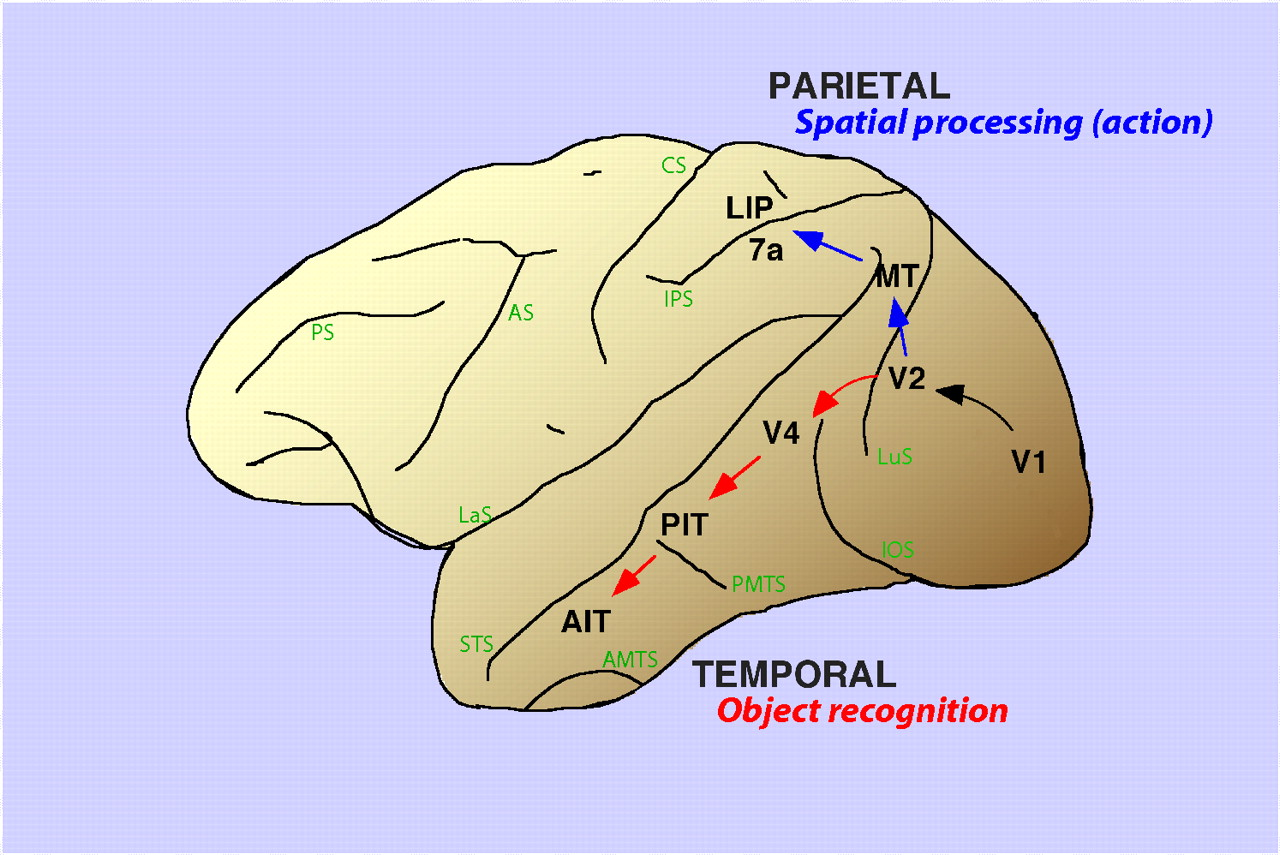
\includegraphics[width=0.8\textwidth]{pics_report/twoPaths.jpg}
	\caption{The dorsal and ventral pathway in the brain~\cite{lehky2007comparison}.
	The dorsal stream (blue) arrives to the parietal lobe, whereas the ventral pathway (red) reaches the inferotemporal (IT) cortex in the temporal lobe.}
	\label{Fig:TwoPath}
\end{figure}
The central visual system consists of several cortical areas responsible for visual processing, which are placed in a hierarchical pattern according to the anatomical experiments~\cite{felleman1991distributed}.
There are two basic streams locating in the visual area: a dorsal and a ventral pathway (Figure~\ref{Fig:TwoPath}).

They differ in behavioural patterns according to the observation from brain lesions~\cite{prado2005two}, and also in functions where the dorsal pathway targets on the `where' tasks and the ventral on the `what'.
The ventral visual stream holds the critical circuits for object recognition and stimulus identification, whereas the dorsal pathway pathway contributes to the processing of the spatial location of the stimulus~\cite{prado2005two, Ungerleider1994157}.
Another definition of the difference between these two pathways is a `perception/action' dichotomy: the ventral (`perception') stream perceives the world by means of object recognition and memory, while the dorsal (`action') stream provides real-time visual guidance for motor actions such as eye movements and grasping objects~\cite{goodale1992separate}. 

This research mainly focuses on the ventral visual pathway, since it dominates the object recognition among the cortical areas.
Thus, the dorsal pathway will beyond the scope of the this study. 


\subsection{Cortical Areas in The Ventral Visual Pathway}
The ventral visual pathway starts from the primary visual cortex V1 in the occipital cortex through areas such as V2 and V4 to the Inferotemporal (IT) cortex.
These cortex areas are divided based on the anatomical experiments and retinotopic maps.
Accordingly, the IT complex is commonly parsed into sub areas such as TEO and TE~\cite{janssen2000selectivity,von1947neocortex} or posterior IT (PIT), central IT (CIT), and anterior IT (AIT)~\cite{felleman1991distributed}.
\subsubsection{Primary Visual Cortex: V1}
As the simplest and earliest cortical area in the ventral stream, the primary visual cortex V1 is the best-studied since the well-known discovery of the orientation selectivity by Hubel and Wiesel~\cite{hubel1959receptive} in 1958.
The retinotopic map is well-defined to transform spatial information from retinal image to V1~\cite{tootell1982deoxyglucose}.
In human and animals with a fovea in the retina, the central 10 degrees of the visual field occupies roughly half of V1.
This distorted retinotopic map in V1 is a phenomenon known as cortical magnification.

\begin{figure}
	\centering
	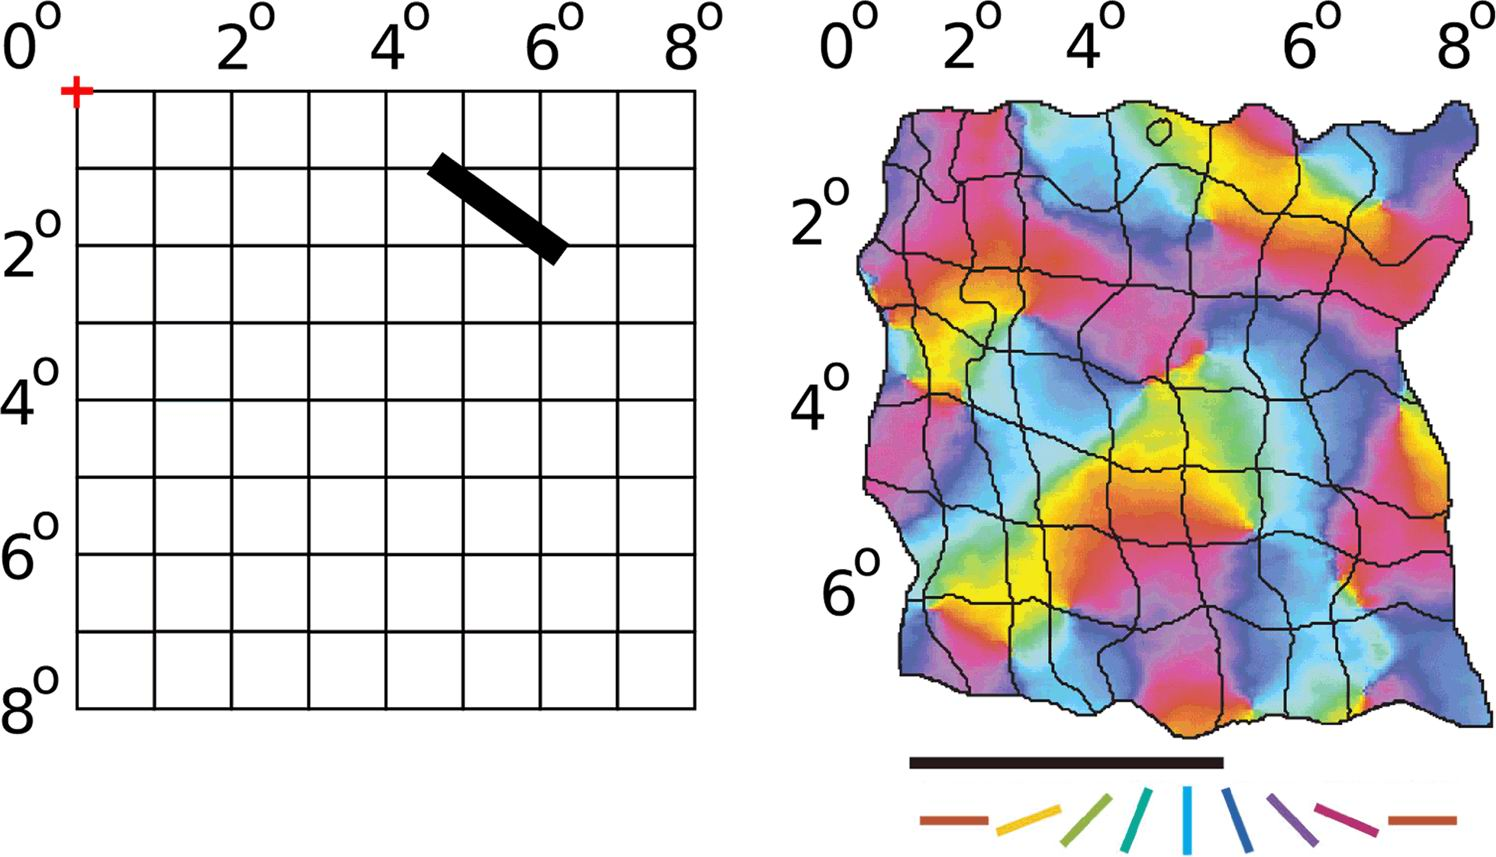
\includegraphics[width=0.8\textwidth]{pics_report/retinotopic.jpg}
	\caption{The retinotopic and orientation map on the surface of V1 of a tree shrew~\cite{bednar2009topographica}.
	The visual field (left) with a fixation point marked as a red cross on the up-left corner can be divided into a regular grid.
	Each square represents a 1$^\circ \times 1^\circ$ area of visual space.
	In cortical area V1 of mammals, neurons are arranged into a retinotopic map (right) responding to the retinal visual space.
	As an example, the retinotopic map shows the orientation preference of the V1 neurons of a tree shrew for an 8$^\circ \times 7^\circ$ area of visual space (adapted from~\cite{bosking2002spatial}; scale bar is 1 mm).}
	\label{Fig:retinotopic}
\end{figure}

In the spatial domain, V1 neurons are tuned to Gabor-like transforms applied to their small local receptive field.
The retinotopic and orientation map on the surface of V1 of a tree shrew is shown in Figure~\ref{Fig:retinotopic}.
A black bar presented in the retinal image evokes a response in the corresponding grid square of V1 (6$^\circ$, 2$^\circ$) depending on the orientation of the stimulus.
The coloured map on the right represents the preferred orientation of neurons in each location.
Thus the black bar shown at left will activate V1 neurons coloured in purple in the specific square.
In theory, these Gabor-like filters together can carry out neuronal processing of spatial frequency, orientation, motion, direction, speed, and many other spatiotemporal features.
Similar maps could be plotted for this same area showing preference for other visual features.

\subsubsection{Prestriate Cortex: V2}
Visual area V2, also called prestriate cortex~\cite{an2012distinct}, is the second major area located in the occipital lobe of the primate brain, and the first region within the visual association area~\cite{wu2011early}. 
It receives strong feed-forward connections from V1 and has many properties in common with V1. 

The responses of V2 neurons are tuned to simple shapes such as orientation and sinusoidal gratings. 
Moreover, V2 neurons are able to represent variety of higher order shapes that are based on contours (e.g., angles and curves with multiple orientations at different subregions within a single receptive field) or grating patterns~\cite{hegde2000selectivity}.
The responses of many V2 neurons are also modulated for complex properties: orientation of illusory contours~\cite{anzai2007neurons}, binocular disparity~\cite{daniel2009whither}, and whether the stimulus is part of the figure or the ground~\cite{qiu2005figure}.

%In a recent study, the Layer 6 cells of the V2 cortex were found to play a very important role in the storage of Object Recognition Memory as well as the conversion of short-term object memories into long-term memories.[23]

\subsubsection{Visual Area V4}
Area V4 is the third cortical area in the ventral stream, receiving strong feedforward input from V2 and transmitting to the PIT.
It also receives direct inputs from V1 which are mostly generated in the visual central space.
V4 is the first area in the ventral stream to show strong attentional modulation.
Most studies indicate that selective attention can change firing rates in V4 by about 20\%~\cite{filipe2013human}.
This discovery found by Moran and Desimone~\cite{moran1985selective} was the first report of attention effects anywhere in the visual cortex.

Although V4 is mainly modulated for colour recognition, it is also tuned for orientation and spatial frequency similar to V1.
Comparing to V1, V4 responds to more complex object features with intermediate complexity but is not tuned for complex objects as areas in the inferotemporal cortex are~\cite{williams2007biological}.

\subsubsection{Inferotemporal Cortex: IT}
Inferotemporal Cortex is only found in the temporal lobe in primates including humans. 
It is tuned to a range of object features complexity starting with simpler patterns in the PIT/TEO~\cite{tanaka1991coding};
And the complexity increases along the ventral stream towards AIT/TE where objects are represented and recognised~\cite{dean1976effects}.
The high-order complex features includes the combinations of colour or texture with complicated shapes~\cite{tanaka1991coding}, and body parts such as faces and hands~\cite{gross2008single}.
The distinguishing features of the IT cortex is that the neuronal responses are position and size invariant~\cite{schwartz1983shape,logothetis1995psychophysical}, and also invariant to changes in luminance, texture, and relative motion ~\cite{sary1993cue,perry2014feature}.
It is wide-accepted that the identity-preserving transformation invariance makes IT ideal for representing objects despite changes in the surrounding environment and retinal image.

In the next section, this report will explore the detailed mechanism of object representation in this cortical area.
%PFC
\subsection{Object Representation in IT}
\label{sec:orIT}
%\subsection{Untangling Object Representation}
The neuronal representation in the cortical area of IT is considered to be the spatio-temporal pattern of spikes.
The spiking activities of single neurons and populations are thought to hold the key to encode visual information.
In Section~\ref{sec:SNNintro}, the report will introduce single neuron models and spike coding mechanisms in computational spiking neural networks.

\subsubsection{Single neurons}

\begin{figure}[b!]
	\centering
	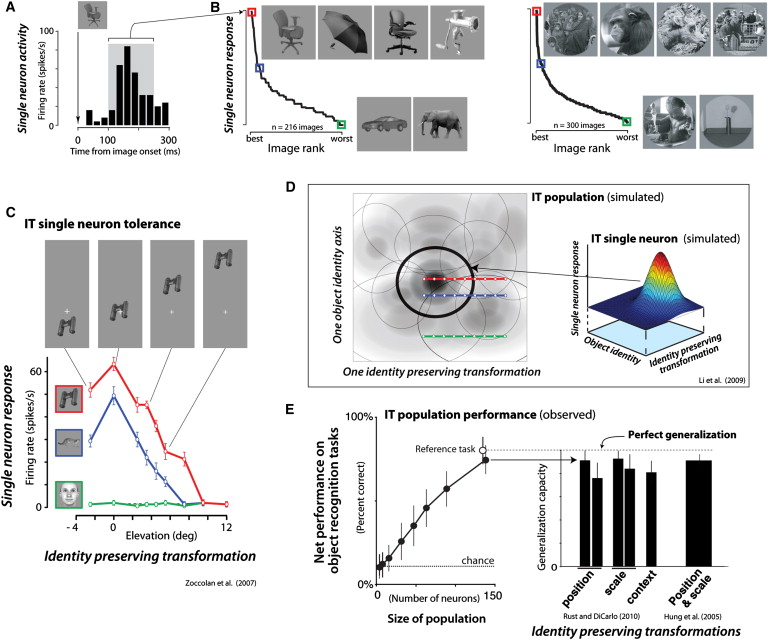
\includegraphics[width=0.9\textwidth]{pics_report/IT.jpg}
	\caption{	
		IT single-neuron properties and their relationship to population performance~\cite{dicarlo2012does}.
	}
	\label{Fig:IT}
\end{figure}
Most studies have investigated the neural activities in the IT by means of firing rate or spike count.
A typical histogram, Figure~\ref{Fig:IT}(A)~\cite{zoccolan2007trade}, shows the spike count of a single neuron in time bins of 25~ms for a duration of 300~ms in total right after the presentation of a visual image.
The highlighted time window, the so-called `decoding' window, is adjusted to the latency of the conductance along the ventral stream. 
The spike count of the `decoding' window is well modulated for object identity, position or size~\cite{desimone1984stimulus,kaneko1996sequence}, see example in Figure~\ref{Fig:IT}(B) where the left shows the spiking activities for clean figures and the right for natural scenes.
The neural responses were sorted from high to low with the corresponding figures presented, where the red point indicated the highest respond while the green the lowest and the blue the medium.
Another example in Figure~\ref{Fig:IT}(C) shows the responses of an example IT neuron obtained by varying the position (elevation) of three objects with high (red), medium (blue), and low (green) activities.
The object identity preference was maintained in the entire test range regardless of the position changes.
These tuning curves are similar to the well-understood firing rate modulation in visual area V1 on the bar orientation.

%A Contemporary View of IT Single Neurons\\
%Respond to different variations\\
%How do these IT neuronal population phenomena (above)
%depend on the responses of individual IT neurons?
Understanding IT single neuron responses has proven to be extremely challenging and even predicting the responses of an IT neuron to a new image remains impossible.
Nevertheless, IT neurons are activated by complex combinations of visual features and that they are often able to maintain their relative object preference over small to moderate changes in object position, scale, pose~\cite{logothetis1996visual}, illumination~\cite{vogels2002effects} and clutter~\cite{zoccolan2005multiple}.

%respond to more objects\\
Although IT neurons are commonly described as narrowly selective object identifier, neurophysiological studies have shown a diverse selectivity of single neurons~\cite{desimone1984stimulus}.
Most IT neurons are broadly tuned and the typical IT neuron responds to many different images and objects~\cite{zoccolan2007trade}, also see Figure~\ref{Fig:IT}(B).
As illustrated in Figure~\ref{Fig:IT}(D), a single neuron (right) is modulated to both object identities and variables of identity-preserving transformations.
To explain the plot in ~\ref{Fig:IT}(C), position is the variable here; thus the tuning curve for different identities on each position can be described as a slice in the 3-D plot which is Gaussian-like.
As a result, the rank order of the three objects remains the same due to the Gaussian-like curve stays similar.
If a population of such IT neurons tiles with the overlapping fashion, see left panel of Figure~\ref{Fig:IT}(D), a more accurate recognition result containing the transformation parameter can be carried out with population coding.

\subsubsection{Population of neurons}

Spike timing variability in the ms resolution of spikes is consistent with a Poisson-like stochastic spike generation process.
The underlying output rate of IT neurons is determined by each particular image.
Despite the timing variability, the brain can reliably recognise the presented object by integrating the neural responses across IT population~\cite{de2007properties}.
However, it still remains unclear whether the spike timing variability brings down the encoding/decoding accuracy or if it contributes to the population tuning for useful informations~\cite{ermentrout2008reliability}. 

%simple weighted summations of IT spike\\
Although the first stage of the ventral stream, V1, is reasonably well studied, the visual processing in higher stages especially in V4 and IT remains poorly understood.
Nevertheless, as stated above IT is the main part of ventral stream to recognise and categorise the objects in real-time and is tolerant to identity-preserving transformations.
Specifically, simple linear classifier built on the output rates of randomly selected population with only a few hundred neurons reveals a high-level of object recognition performance~\cite{hung2005fast};
and the simple weighted summation explains a wide range of invariant object recognition behaviour sufficiently~\cite{majaj2012unified}.

Figure~\ref{Fig:IT}(E) shows the direct tests of measuring the cross-validated population performance on categorisation tasks using linear classifiers.
The recognition performance approaches ceiling level with only a few hundred neurons (left panel), and the same population shows a good generalization across moderate changes in position, scale, and context.
%50 ms window matters\\
\subsubsection{Decoding Window Matters}
The output spiking pattern of the ventral visual stream are well described by a firing rate code where the decoding window size is 50~ms~\cite{hung2005fast}.
Thus the visual representation in IT is usually found in the first 50~ms of neuronal response, although different time epochs relative to stimulus onset may encode different types of visual information~\cite{brincat2006dynamic} (see Figure~\ref{Fig:IT}(A), an appropriate decoding window can be 100-150~ms after image onset).

%\subsection{IT}




%conclusion\\
%Such findings argue for a distributed representation of visual
%objects in IT, as suggested previously (e.g., Desimone et al.,
%1984; Kiani et al., 2007; Rolls and Tovee, 1995)—a view that
%motivates the population decoding approaches described
%above (Hung et al., 2005; Li et al., 2009; Rust and DiCarlo,
%2010). That is, single IT neurons do not appear to act as sparsely
%active, invariant detectors of specific objects, but, rather, as
%elements of a population that, as a whole, supports object recog-
%nition. This implies that individual neurons do not need to be
%invariant. Instead, the key single-unit property is called neuronal
%‘‘tolerance’’: the ability of each IT neuron to maintain its prefer-
%ences among objects, even if only over a limited transformation
%range (e.g., position changes; see Figure 4C; Li et al., 2009).
%Mathematically, tolerance amounts to separable single-unit
%response surfaces for object shape and other object variables
%such as position and size (Brincat and Connor, 2004; Ito et al.,
%1995; Li et al., 2009; Tove ́e et al., 1994; see Figure 4D). This
%contemporary view, that neuronal tolerance is the required and
%observed single-unit phenomenology, has also been shown for
%less intuitive identity-preserving transformations such as the
%addition of clutter (Li et al., 2009; Zoccolan et al., 2005).


%Summery\\
%Taken together, the neurophysiological evidence can be
%summarized as follows. First, spike counts in 50 ms IT decod-
%ing windows convey information about visual object identity.
%Second, this information is available in the IT population begin-
%ning 100 ms after image presentation (see Figure 4A). Third,
%the IT neuronal representation of a given object across changes
%in position, scale, and presence of limited clutter is untangled
%from the representations of other objects, and object identity can
%be easily decoded using simple weighted summation codes (see
%Figures 2B, 4D, and 4E). Fourth, these codes are readily
%observed in passively viewing subjects, and for objects that
%have not been explicitly trained (Hung et al., 2005). 

In sum, the output of the ventral stream is reflexively expressed in neuronal firing rates across a short interval of 50 ms and is an explicit object representation;
and the rapid production of this representation is consistent with a largely feed-forward, non-linear processing of the visual input~\cite{dicarlo2012does}, which is described in the following section.
\subsection{Hierarchical Feed-forward Organisation }
%Feed-forward, hierarchical organisation and abstraction.

\begin{figure}[h!]
	\centering
	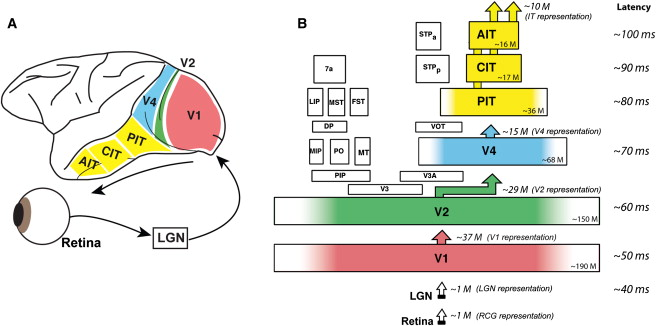
\includegraphics[width=0.9\textwidth]{pics_report/ventral.jpg}
	\caption{The ventral visual pathway and its hierarchical organization~\cite{dicarlo2012does}.
}
	\label{Fig:Ventral}
\end{figure}
Figure~\ref{Fig:Ventral}(A) illustrates the ventral stream cortical area locations in the macaque monkey brain, and the flow of visual information from the retina.
The corresponding hierarchical organisation is showed in Figure~\ref{Fig:Ventral}(B).
Each area is plotted with the size proportional to its cortical surface size.
Approximate total number of neurons of both hemispheres is shown in the corner of the cortical areas.
The approximate number of projections is written above each block.
In addition, the colour dedicates to processing the central 10$^\circ$ of the visual field.
At last, approximate median response latency is listed on the right.
%of the ventral stream with spikes travelling first from the retina to the lateral geniculate nucleus of the thalamus (LGN), and then through cortical areas introduced above: V1 , V2, V4 to IT. 
\subsubsection{Latency}
Each cortical area along the ventral stream contributes a conductance latency of about 10~ms of the visual information~\cite{nowak1997timing}.
Thus, just around 100~ms after images appeared in front of the retina, a first wave of object identity neuronal activity is present throughout much of IT (e.g., Figure~\ref{Fig:IT}(A)).

\subsubsection{Neurons and Connections}
Because retinal and LGN receptive fields are point-wise spatial sensors, the object visual information conveyed to V1 are nearly as raw as the pixel representation (1 million pixels). 
As V1 carries out its visual process, the total object representation increases approximately 30-times~\cite{stevens2001evolutionary} because of its non-linear filtering.
This dimensionality expansion results in an overcomplete population re-representation~\cite{lewicki2000learning} in which the object representation vectors have more dimensions than the LGN input.
As a result, simulations show that a V1-like representation is clearly better than RGN-like/pixel-based representation, but still far below human performance for real-world recognition problems~\cite{dicarlo2007untangling}.

The output projections of each area decreases from V2 (about 29 million) to AIT which represents the object with 10 million dimensions.
At the same time, the receptive field size of neurons increases to complete the object representation with a whole image and to perform invariant recognition.

%\begin{figure}
%	\centering
%	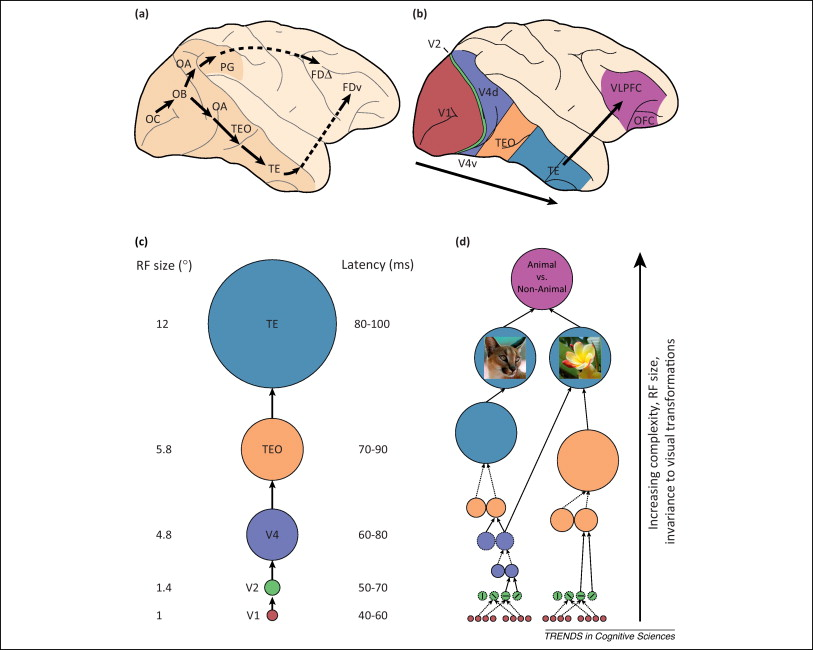
\includegraphics[width=0.9\textwidth]{pics_report/hierarchi.jpg}
%	\caption{Receptive field sizes of the sub areas along the hierarchical visual processing pathway~\cite{kravitz2013ventral}.}
%	\label{Fig:Hir1}
%\end{figure}
\subsubsection{Tuned Features and Receptive Fields }
\begin{figure}[h!]
	\centering
	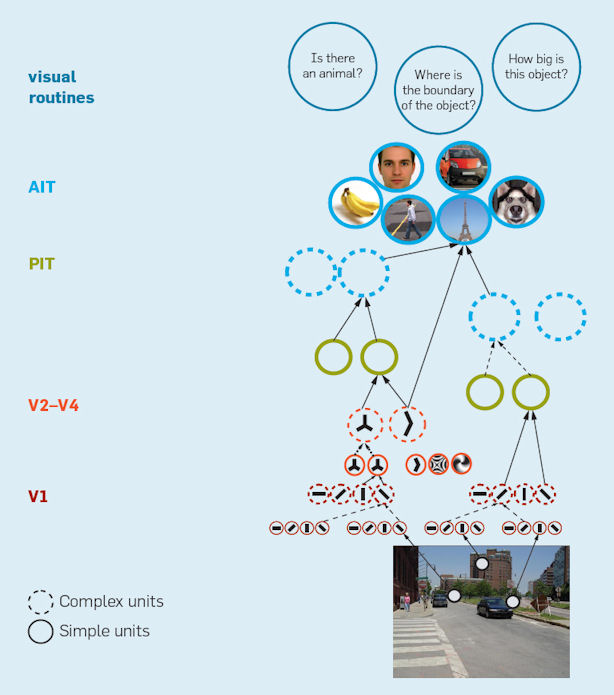
\includegraphics[width=0.9\textwidth]{pics_report/serre.jpg}
	\caption{The hierarchical ventral stream and the corresponding tuned features for each layer~\cite{serre2010neuromorphic}.}
	\label{Fig:serre}
\end{figure}
As the visual information conducts along the ventral stream, neurons become selective for stimuli that are increasingly complex from simple oriented bars and edges in early visual area V1 to moderately complex features in intermediate areas: V2, V4 and PIT to complex objects and faces in AIT, see Figure~\ref{Fig:serre}.
Along with this growing complexity of the preferred stimulus, the invariance properties of neurons also increase.
Neurons become more and more tolerant with respect to the exact position and scale of the stimulus within their receptive fields.
As a result, the receptive field size of neurons increases from
about one degree or less in V1 to several degrees in IT, see Figure~\ref{Fig:Hir1}.

\begin{figure}[h!]
	\centering
	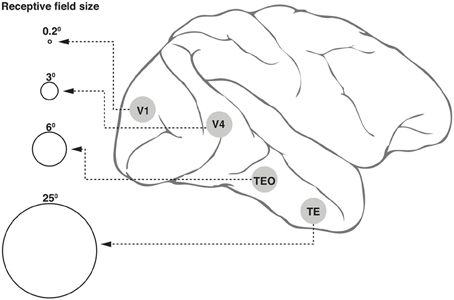
\includegraphics[width=0.6\textwidth]{pics_report/rf.jpg}
	\caption{Receptive field (RF) sizes along the ventral cortical stream in the primate. While the degree of complexity of processing may increase, the RF size at any one eccentricity also increases dramatically along the various cortical areas from V1 into the temporal pole. The circles shown in the figure are not drawn to scale, but the numbers above the circles indicate approximate relative sizes of the RF diameters.~\cite{vidyasagar2013reading}.}
	\label{Fig:Hir1}
\end{figure}

%\subsubsection{Tuned Features}
%
%V1 are orientation selective for multiple stimulus types, i.e., edges, bars, gratings (Hubel and Wiesel, 1968; Hubel et al., 1978).
%V2 cells encode border ownership (Zhou et al., 2000) which is the first stage of assigning an oriented edge to an object representation.
%Thus contour-based object representation starts in V2.
%Form processing in V4 combines multiple, spatially-adjacent, orientation responses seen in V1 and V2 to encode angles and curvatures (Pasupathy and Connor, 1999).
%These responses advance the nascent object representation from border ownership (Orban, 2008) to responses that are dependent on the placement of the curvature with respect to the center of the shape (Pasupathy and Connor, 2001).
%
%Inferior temporal (IT) cortex has a range of object property complexity starting with simpler features posteriorly (PIT or TEO: Tanaka et al., 1991; Kobatake and Tanaka, 1994) that increase in complexity as processing moves anteriorly (AIT or TE) to represent objects and perform object recognition (Cowey and Weiskrantz, 1967; Gross et al., 1971, 1972; Dean, 1976).
%This includes complex shapes, combinations of color or texture with shape (Gross et al., 1972; Desimone et al., 1984; Tanaka et al., 1991), and body parts (faces or hands: see Gross, 2008 for a review). 
%In addition, responses in IT cortex are position and size invariant (Sato et al., 1980; Schwartz et al., 1983; Rolls and Baylis, 1986; Ito et al., 1995; Logothetis and Pauls, 1995) and also invariant to changes in luminance, texture, and relative motion (Sáry et al., 1993).
%Combined, these characteristics make IT ideal for representing objects despite changes in the surrounding environment and retinal image.

%
%\begin{figure}
%	\centering
%	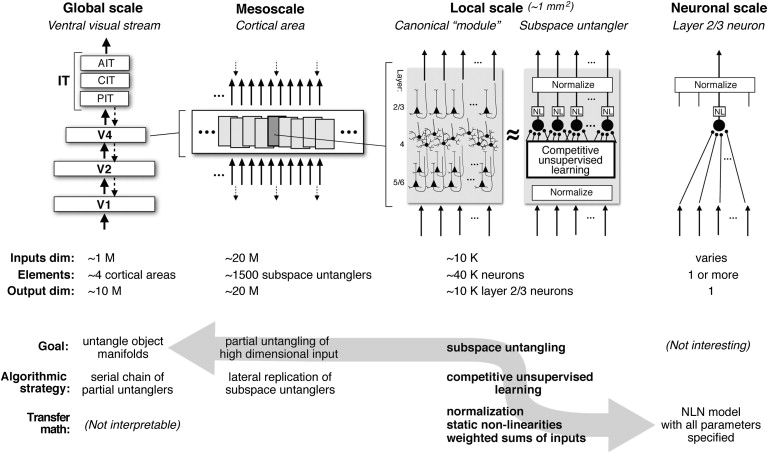
\includegraphics[width=0.9\textwidth]{pics_report/hierarchiNLN.jpg}
%	\caption{The ventral visual pathway and its hierarchical organization~\cite{dicarlo2012does}.}
%	\label{Fig:HirNLN}
%\end{figure}

\section{Computational Neuroscience: what and why spiking neurons}
\label{sec:comp}

%\section{Spatial Temporal Learning}
%\label{sec:stl}
The so-called third generation of neural networks~\cite{maass1997networks} introduces a different set of functions and parameters to model neurons;
%these both model biological neurons more precisely~\cite{hodgkin1952quantitative} and increase the computational power of networks of neurons if compared to classical sigmoidal units.
it models the biological neurons more precisely and increases the computational power of neural networks when compared to the classical sigmoid functions.
Such networks rely on the propagation of an all-or-none signal, the action potential, which asynchronously carries information to its connected units by means of its timing.
\subsection{Neuronal Model}
Spiking neuron models can be divided into two major categories \cite{gernstbook} based on their level of abstraction: The conductance models and the threshold models.
The conductance models simulate a lower level on the ion channels, while the threshold models represent a higher level of neuron abstraction where the threshold voltage is fixed and the neuron fires once the membrane potential reaches it.

In general, Conductance-Based models have been derived from the Nobel prize winners (1963) Hodgkin and Huxley, based on the experiments that they performed on the giant axon squid \cite{hhmodel}.
Spikes arriving at a LIF neuron cause a temporary flow of current into (excitatory synapse) or out of (inhibitory synapse) the neuron, modelling the behaviour of synapses in biological neurons.
The LIF neuron sums up this current over time, accumulating charge which gradually leaks away.
If the membrane potential in the neuron reaches a certain threshold, it produces a spike and its charge is reset.
LIF neurons have been extensively used in large spiking neural networks \cite{Delorme1999989} because of their ease of implementation and the low computational cost.

\subsection{Learning}
%One of the key parameters of a neural network is the amount of influence each incoming spike has on a neuron.
The influence each incoming spike has on a post-synaptic neuron is modelled by assigning a `weight' to each synapse;
tuning on the weight scales the impact of a spike
arriving via that synapse.
Many learning models simulate the changes in weights over long periods of time observed within the brain.
The exact rules by which these weights are adjusted is the subject of much active research though most promising approaches attempt to learn from the relative timing \cite{pfister2006triplets} or rate \cite{bienenstock1982theory} of spikes arriving at a neuron.
As well as adjusting weights, some learning rules can also form entirely new connections between previously unconnected
neurons \cite{bamford2010synaptic}.

\section{Neuromorphic Engineering}
\label{sec:morph}

\section{Deep Learning}
\subsection{Convolutional Network}
\subsection{Autoencoders}
Figure~\ref{fig:AE} shows a simplest architecture of an autoencoder, which is the same as a multilayer perceptron (MLP).
The only difference lies to the number of the output units, where an autoencoder has as many output neurons as the input.
In this example, the input layer feeds forward the data vector $\mathbf{v}$ to the hidden layer as weighted sum of the data, $\mathbf{net\_h}$.
Then the hidden units are activated by the input $\mathbf{net\_h}$ according to the activation function: $\mathbf{h}=\sigma(\mathbf{net\_h})$.
Finally, using the same approach the output of the network is generated, $\mathbf{v'}=\sigma(\mathbf{net\_v'})$, as the reconstruction of the input data.
Thus, autoencoders are trained without given target values, work as unsupervised learning models.
\begin{equation}
h_j=\sigma(\sum_i v_i w^T_{ij})
\end{equation}
\begin{equation}
v'_j=\sigma(\sum_i h_i w_{ij})
\end{equation}

\begin{figure}
	\centering
	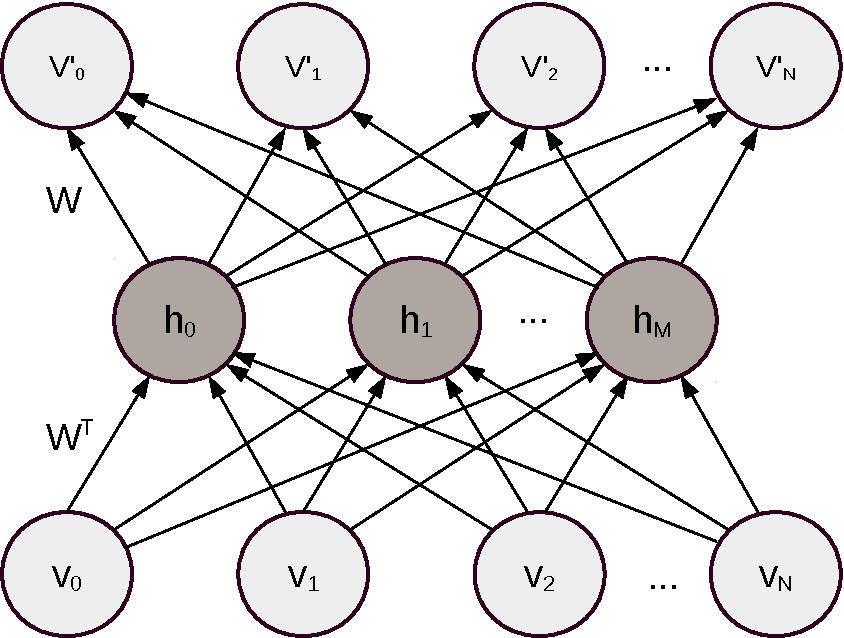
\includegraphics[width=0.5\textwidth]{pics_sdlm/AE.pdf}
	\caption{A typical Autoencoder structure.}
	\label{fig:AE}
\end{figure}

%TODO why tied weights are good
Notice that the connections used in the example are tied weights.

Training an autoencoder is not different from backpropagation (BP) on an Multi-Layer Perceptrons(MLP).
The objective of training is to minimise the prediction error of an MLP, which measured as a loss function.
Accordingly, the loss function of an autoencoder can be described as:
\begin{equation}
L=\sum_{k=1}^{K}\|\mathbf{v}_{k}-\mathbf{v'}_{k}\|=\frac{1}{2}\sum_{k=1}^{K}(\mathbf{v}_{k}-\mathbf{v'}_{k})^{2}
\end{equation}
where k indicates the index of the training data $\mathbf{v}$, and each data vector $\mathbf{v}=\{v_0, v_1,...,v_N\}$ and its reconstruction $\mathbf{v'}=\{v'_0, v'_1,...,v'_N\}$ have N dimensions. 

%TODO rewording
Backpropagation, an abbreviation for "backward propagation of errors", is a common method of training artificial neural networks used in conjunction with an optimization method such as gradient descent.
The method calculates the gradient of a loss function with respect to all the weights in the network.
The gradient is fed to the optimisation method which in turn uses it to update the weights, in an attempt to minimize the loss function:
\begin{equation}
\Delta W \propto -\frac{\partial L}{\partial W}.
\end{equation}

Applying stochastic gradient descent (SGD), the true gradient of the weight matrix, $\Delta W$, is approximated by a gradient at a single example with iterations.
The reconstruction error $E_k$ of an input vector $\mathbf{v}_k$ is as given:
\begin{equation}
%	\begin{align*}
E_k = \frac{1}{2}(\mathbf{v}_k - \mathbf{v'}_k)^2,
%	\end{align*}
\end{equation}
and the gradient of the weight matrix is:
\begin{equation}
\Delta W \propto -\frac{\partial E_k}{\partial W}=-\eta \frac{\partial E_k}{\partial W},
\end{equation}
where $\eta$ is the learning rate.

Since we use tied weights in the network, the weight tuning only needs to apply in the output layer.
\begin{equation}
\begin{aligned}
\Delta w_{ij} = -\eta \frac{\partial E_k}{\partial w_{ij}} &= -\eta \frac{\partial E_k}{\partial v'_j} \frac{\partial v'_j}{\partial net\_v'_j} \frac{\partial net\_v'_j}{\partial w_{ij}}, \textrm{ where} \\
\frac{\partial E_k}{\partial v'_j} &= \frac{\partial \frac{1}{2}(\mathbf{v}_k - \mathbf{v'}_k)^2}{\partial v'_j}= -(v'_j - v_j), \\
%	\frac{\partial v'_j}{\partial net\_v'_j} &= \begin{cases} 1, v'_j>0\\0, v'_j<=0\\ \end{cases}, \textrm{using ReLU,}\\
\frac{\partial v'_j}{\partial net\_v'_j} &= 1, \textrm{using Identify function,}\\
\frac{\partial net\_v'_j}{\partial w_{ij}} &= \frac{\partial h_i w_{ij}}{\partial w_{ij}} = h_i.
\end{aligned}
\end{equation}
Thus, the weight gradient is calculated as:
\begin{equation}
\Delta w_{ij} = \eta h_i(v'_j - v_j)
\end{equation}

\subsection{Restricted Boltzmann Machine}
\subsection{Restricted Boltzmann Machine}
In order to implement training and testing of Spiking Deep~Belief~Networks~(SDBNs) on-line, this section studied:
\begin{itemize}
	\item \textit{Contrastive Divergence.}
	The study starts from understanding the original problem, Products of Experts~(PoE), which was solved by using Contrastive~Divergence~(CD).
	It involves utilising Markov~Chain~Monte~Carlo~(MCMC) sampling to present the distribution of a certain untraceable high-dimensional probability model function, e.g. PoE.
	Among these sampling algorithms, Gibbs method is introduced and used in high dimensional problems.
	Instead of minimising the original objective function of Kullback-Leibler divergence, the contrastive divergence is exploited to solve PoE.
	\item \textit{Restricted Boltzmann Machine (RBM). }
	Then the study continues on applying Gibbs sampling and CD to RBM, which builds the foundation of the light RBM training.
	\item \textit{Deep Belief Network.} 
	The greedy algorithm on training layered RBMs and the fine training on the whole DBN are studied.
\end{itemize}
Next, the study will carry on to on-line learning methods which only applies to spiking neurons for training spiking RBM and DBN.
\subsubsection{Contrastive Divergence\cite{hinton2002training,woodfordnotes}}
The probability of a vector point $ \mathbf{x} $ is modelled by the function $f(\mathbf{x} \mid \Theta )$ given the model parameters $ \Theta $, and normalised by a partition function $Z( \Theta)$:

\begin{equation}
p(\mathbf{x} \mid \Theta ) = \dfrac{f(\mathbf{x} \mid \Theta )}{Z( \Theta)}
\end{equation}
where the partition function is defined as:
\begin{equation}
\label{equ:z_int}
Z( \Theta) = \int f(\mathbf{x} \mid \Theta )\D\mathbf{x}, \text{when  $ \mathbf{x} $ is continuous, or}
\end{equation}

\begin{equation}
\label{equ:z_dis}
Z( \Theta) = \sum_{\mathbf{x}} f(\mathbf{x} \mid \Theta ), \text{when  $ \mathbf{x} $ is discrete.}
\end{equation}
Given a set of data points $ \mathbf{D}=(\mathbf{d}_1, \mathbf{d}_2, ..., \mathbf{d}_K) $ the purpose of learning is to tune the model parameter $ \Theta $ to fit the data $ \mathbf{D}  $. 
The objective function is the probability product of all the independent data points of the data set, which is also called the likelihood function:
\begin{equation}
L (\Theta \mid \mathbf{D}) = p(\mathbf{D} \mid \Theta ) = \prod_{k=1}^K p(\mathbf{d}_k \mid \Theta ) =  \prod_{k=1}^K\dfrac{f(\mathbf{d}_k \mid \Theta )}{Z( \Theta)}.
\end{equation}
And the target is to maximise the likelihood given the data set $ \mathbf{D}  $, which equals to maximise the log of the probability product (the log-likelihood):
\begin{equation}
\log  L (\Theta \mid \mathbf{D}) = \log p(\mathbf{D} \mid \Theta ) = \sum_{k=1}^K\log f(\mathbf{d}_k \mid \Theta ) - K \log Z( \Theta),
\end{equation}
or the average log-likelihood:
\begin{equation}
\label{equ:like}
\hat{l} (\Theta \mid \mathbf{D}) =\frac{1}{K}\log  L (\Theta \mid \mathbf{D}) 
=\frac{1}{K}\sum_{k=1}^K\log f(\mathbf{d}_k \mid \Theta ) - \log Z( \Theta).
\end{equation}
Imagine three different conditions (probability function) as following.

\textbf{First}, $f(\mathbf{x} \mid \Theta )$ is the probability density function (pdf) of a normal distribution $\mathcal{N}(x \mid \mu, \sigma )$.
Data vector $ \mathbf{x} $ is just a one dimensional data point, $x$.
$ Z( \Theta) $ equals to 1, thus $p(x \mid \Theta ) = \mathcal{N}(x \mid \mu, \sigma )$.
\begin{equation}
\hat{l} (\Theta \mid D) =  
\frac{1}{K} \sum_{k=1}^K \log \left[ \frac{1}{\sigma \sqrt{2\pi}} \exp(-\frac{(d_k-\mu)^{2}}{2\sigma^{2}}) \right]
\label{pdf}
\end{equation}
To maximise Equation~\ref{pdf} is to find the Maximum Likelihood Estimation (MLE) of parameters $ \mu $ and $ \sigma $, by deriving from the partial differential equations when they are equal to 0. 
\begin{equation}
\left\{
\begin{aligned}
&\dfrac{\partial \hat{l} (\Theta \mid D)}{\partial \mu}= \sum_{k=1}^K -\frac{1}{2\sigma^{2}}\dfrac{\partial (\mu-d_k)^{2}}{\partial \mu} = \sum_{k=1}^K -\frac{1}{\sigma^{2}}(\mu-d_k) = 0 \quad\\
&\dfrac{\partial \hat{l} (\Theta \mid D) }{\partial \sigma^{2}}= -\frac{K}{2\sigma^{2}}+\frac{1}{2\sigma^{4}}\sum_{k=1}^K d_k^{2} -\frac{\mu}{\sigma^{4}}\sum_{k=1}^K d_k + \frac{K\mu^{2}}{2\sigma^{4}} = 0 \quad\\
\end{aligned}
\right.
\end{equation}
\begin{equation}
\left\{
\begin{aligned}
&\mu= \frac{1}{K}\sum_{k=1}^K d_k  \quad\\
&\sigma^{2} = \frac{1}{K}\sum_{k=1}^K d_k^{2} - (\frac{1}{K}\sum_{k=1}^K d_k)^{2}
\end{aligned}
\right.
\end{equation}
$\hat{l} (\Theta \mid D)$ here is the function of two dimensional parameters $\mu$ and $\theta$, and searching the highest point in the parameter space ``is equivalent to being in the field on a clear, sunny day,''~\cite{woodfordnotes} seeing the point straight away.

\textbf{Second}, the probability model function changes to be the sum of N normal distributions: 
\begin{equation}
f(x \mid \Theta ) = \sum_{i=1}^N\mathcal{N}(x \mid \mu_i, \sigma_i ).
\end{equation}
Derived from Equation~(\ref{equ:like}), the objective function is:
\begin{equation}
\hat{l} (\Theta \mid D) = \frac{1}{K}\sum_{k=1}^K \log \sum_{i=1}^N \mathcal{N}(d_k \mid \mu_i, \sigma_i ) - \log N,
\end{equation}
where $\log Z( \Theta)$ still equals a constant, but the partial differential equation of any parameter depends on other model parameters.
It is very hard to solve equation set of log of sum, thus iteration methods are introduced, e.g., gradient descent method. %and expectation maximization (EM) algorithm
Searching for a local maximum of the likelihood function in the parameter space starts with an initial point, either random or well selected.
For each iteration, the partial derivatives for every dimension of the parameter point are calculated as the gradient.
The gradient determines the decent direction of the space search, the next parameter point is one step $ \eta $  towards the direction or is the highest point found by line search.

The gradient descent method is equivalent to ``being in the field at night with a torch.''~\cite{woodfordnotes}.
And then the descent direction is estimated and chosen by using the torch to see the relative heights of the field a short distance in each direction.
Because partial differential equation of any parameter depends on other model parameters, we can only see the gradient for a small area.
The search will follow the direction by walking one step or a certain distance (e.g. line search lowest point), and then start a new iteration.

\paragraph{PoE Problem} 
%\subsubsubsection{PoE Problem}
\textbf{Finally}, the probability model function becomes the product of N normal distributions: 
\begin{equation}
f(x \mid \Theta ) = \prod_{i=1}^N\mathcal{N}(x \mid \mu_i, \sigma_i ),
\end{equation}
where the partition (normalisation) function $Z( \Theta)$ is no longer a constant, but varies accordance to all the parameters.
Essentially, the integration of the probability model, see Equation~(\ref{equ:z_int}) and~(\ref{equ:z_dis}), is usually algebraically intractable.
We have to use numerical integration method to evaluate the Equation~(\ref{equ:like}), whose partial derivative is (we are using vectors to generalise the problem):
\begin{equation}
\label{equ:part}
\begin{aligned}
\dfrac{\partial \hat{l} (\Theta \mid \mathbf{D})}{\partial \theta} 
& = \frac{1}{K} \dfrac{\partial \sum_{k=1}^K\log f(\mathbf{d}_k \mid \Theta )}{\partial \theta} - \dfrac{\partial \log Z( \Theta)}{\partial \theta}\\
& =  \frac{1}{K}\sum_{k=1}^K \dfrac{\partial \log f(\mathbf{d}_k \mid \Theta)}{\partial \theta} - \int p(\mathbf{x} \mid \Theta) \dfrac{\partial \log f(\mathbf{x} \mid \Theta)}{\partial \theta} \D \mathbf{x}\\
& = \left \langle \dfrac{\partial \log f(\mathbf{d} \mid \Theta)}{\partial \theta}\right \rangle_{\mathbf{D}} -\left \langle \dfrac{\partial \log f(\mathbf{c} \mid \Theta)}{\partial \theta}\right \rangle_{\mathbf{C} \sim p(\mathbf{x} \mid \Theta)}  \\
&=\left \langle \dfrac{\partial \log f(\mathbf{x} \mid \Theta)}{\partial \theta}\right \rangle_{\mathbf{X}_{data}} - \left \langle \dfrac{\partial \log f(\mathbf{x} \mid \Theta)}{\partial \theta}\right \rangle_{\mathbf{X}_{model}},
\end{aligned}
\end{equation}
where  $ <\cdot>_x $ denotes the mean expectation of $ \cdot $ given distribution of $x$.
The first term of the right-hand side is easy to get with the given data set $ \mathbf{D} $, and the second term can be approximated by generating data samples $ \mathbf{C} $ according to $ p(\mathbf{x} \mid \Theta) $.
These generative samples is called ``fantasy data'' and can be generated using Monte Carlo Markov Chain (MCMC) sampling, see section~\ref{sec:mcmc}.
The detailed derivation process can be found in Appendix~\ref{app:part}.
Although in this example the integration of product of normal distribution is still tractable, it is also helpful to use numerical integration.

Go back to the metaphor of the parameter field, solving PoE problem is like searching the highest point in a completely dark night without a torch.
The computation of Equation~(\ref{equ:part}) is to ``feel the gradient of the field under our feet''.~\cite{woodfordnotes}.
%The motivation underlining Contrastive Divergence algorithm is to boost the training speed of a Markov Chain in order to represent the distribution of a PoE (Product of Expert) model.
%Thus the sampling can be followed using this trained Markov Chain model. 

\paragraph{MCMC Sampling}
%\subsubsubsection{MCMC Sampling}
\label{sec:mcmc}
In order to solve the integration of algebraically intractable equations we can use numerical integration to approximate.
One of the popular method is Monte Carlo integration:
\begin{equation}
\int_{a}^{b} f(x) \D x = \int_{a}^{b}\frac{f(x)}{q(x)}q(x)\D x = \dfrac{1}{N}\sum_{i=1}^{N}\frac{f(x_i)}{q(x_i)}.
\end{equation}
The integration of $ f(x) $ transforms to the integration of a new function $ F(x) = f(x)/q(x)  $ times its probability function $ q(x) $.
It could be approximated by sampling N data points $ x_i $ according to the probability distribution $ q(x) $, and calculate the average of $ F(x_i) $ as $ <F(x)>_{q(x)}$.
So the main question following is how to sample from a probability distribution.

MCMC algorithm was proposed by Metropolis in 1953 and it became a wide-used sampling method.
The stationary distribution $ \pi $ exists when every two nodes in a Markov Chain are connected regardless of the initial state distribution $ \pi_0 $:
\begin{equation}
\begin{aligned}
&\pi(j) = \sum_{i=1}^{\infty}\pi(i)P_{ij} \\
&\pi P = \pi,
\end{aligned}
\end{equation}
where $ P $ is the transition probability matrix, and $ \pi $ is in the state space of a MC and the sum, $ \sum_{i=1}^{\infty}\pi(i) $,of a state distribution is 1.
Thus based on the useful theorem of MC, sampled sequence $ \{x_0, x_1, ..., x_n, ... \}$ from a MC complies with its stationary distribution $ \pi(x) $.
Metropolis stated that if a MC has a stationary distribution, $ q(x) $, which is exactly needed to sample from, then we can easily obtain a sample sequence along the MC according to the transformation probability matrix $ P $.
Here so far we are describing the MC with discrete states, however the it also applies to continuous $ \pi $ and $ P $.
The problem here is to build $ P $ to make the stationary distribution equal to the required probability, $ \pi(x) = q(x) $.

So the other useful theorem (detailed balance) lies here, if an aperiodic MC is reversible: $\pi (i) P_{ij} = \pi (j) P_{ji},$ then $ \pi $ is the stationary distribution.
It is a stronger condition than the previous theorem, so most of the MCs are not generally eligible:
\begin{equation}
\pi (i) P_{ij} \neq \pi (j) P_{ji}.
\end{equation}
Thus we can introduce another parameter matrix, $ \alpha $ to make a general MC reversible:
\begin{equation}
\pi (i) P_{ij} \alpha_{ij} = \pi (j) P_{ji} \alpha_{ji}	,
\end{equation}
where $ \alpha_{ij} = \pi(j) P_{ji} $ and $ \alpha_{ji} = \pi(i) P_{ij}$.
The altered transformation probability matrix is $ P'_{ij} =  P_{ij} \alpha_{ij}$ and $ P'_{ji} =  P_{ji} \alpha_{ji}$, and the MC complies the detailed balance condition: $\pi (i) P'_{ij} = \pi (j) P'_{ji}$.
The matrix parameter $ \alpha $ is called as ``acceptance rate'', and its physic meaning is as follows: when state $ i $ transforms to state $ j $ with a probability of $ P_{ij} $, the transformation is accepted by the rate of $ \alpha_{ij} $.
Since the accept rate may be too low for the sampling to move along the MC, we can normalise the $ \alpha $ pair to 1:
\begin{equation}
\alpha^{'}(i,j) = min \left\{\frac{\pi(j)P_{ji}}{\pi(i)P_{ij}},1\right\}.
\end{equation}
The algorithm is called Metropolis-Hastings and described in following:
\begin{algorithm}[h]
	\caption{Metropolis-Hastings Sampling}
	\label{alg:mcmc}
	\begin{algorithmic}
		
		%	    \Procedure{Correction}{coeffs $C$, correlations $Q$}
		\State Initialisation $x_0 = s_{random}$, \Comment{$ x $:sampling sequence and $s$:state in MC}
		\For{$t=1, 2, ..., N$}
		\State $y \sim p_(x \mid x_{t-1})$ 
		\Comment{Random drawing the next state by the transformation probability matrix $P$}
		\State $ u \sim Uniform[0,1] $ 
		\Comment{Random drawing from a uniform distribution}
		\If {$ u < \alpha^{'}(x_{t-1},y) = min \left\{\frac{q(y)p_(x_{t-1} \mid y)}{q(x_{t-1})p_(y \mid x_{t-1})},1\right\} $}
		\State {$x_t = y$} \Comment{Accept the transformation when the random number is less than $\alpha$}
		\Else \State {$x_t = x_{t-1}$}  \Comment{Transformation is refused elsewise}
		\EndIf
		\EndFor
	\end{algorithmic}
\end{algorithm}

The probability model function as the product of N normal distributions can be approximated by using this Metropolis-Hastings sampling.

\paragraph{Gibbs Sampling}
%\subsubsubsection{Gibbs Sampling}
\label{sec:Gibbs}
For high dimensional data sampling, it is possible to make the accept rate to 1 which increases the convergence speed dramatically.
According to conditional probability:
\begin{equation}
P(A \mid B) = \frac{P(A \cap B)}{P(B)}.
\end{equation}
For a $ n $ dimensional data $ (\mathbf{x}, y) $ where $ \mathbf{x}=(x_1,x_2,...,x_{n-1}) $, the joint probability of $p(\mathbf{x},y)$ is:
\begin{equation}
p(\mathbf{x},y) = p(y \mid \mathbf{x})p(\mathbf{x}).
\end{equation}
Thus, during sampling if we restrict the direction of transformation to one single axis(dimension), $ y $, from point $ A(\mathbf{x}_1, y_1) $ to point $ B(\mathbf{x}_1, y_2)$:
\begin{equation}
p(\mathbf{x}_1, y_1)p(y_2 \mid \mathbf{x}_1) = p(\mathbf{x}_1, y_2)p(y_1 \mid \mathbf{x}_1) = p(\mathbf{x}_1)p(y_1 \mid \mathbf{x}_1)p(y_2 \mid \mathbf{x}_1),
\end{equation}
then, the MC obeys the condition of detailed balance.
So the stationary distribution $ \pi(x_1,x_2,...,x_n) $ equals to the joint probability $ p(x_1,x_2,...,x_n) $ and the transformation probability matrix P is consisted of the conditional probability of each dimension $ k $ $,  p(x_k \mid x_1,...,x_{k-1},x_{k+1},...,x_n) $.
Therefore, given the conditional distribution of each variable for a multivariate distribution Gibbs sampling is able to approximate the joint distribution with long enough sample sequence.
Gibbs sampling is described as follows:
\begin{algorithm}[h]
	\caption{Gibbs Sampling}
	\label{alg:gibbs}
	\begin{algorithmic}
		
		%	    \Procedure{Correction}{coeffs $C$, correlations $Q$}
		\State Initialisation $\mathbf{x}_0 = [x_0(1),x_0(2),...,x_0(M)]$,  \Comment{Random initialise $\mathbf{x}_0$}
		\For{$t=1, 2, ..., N$}
		\For{$k=1, 2, ..., M$}
		\State $ x_t(k) = p(x(k) \mid x_{t-1}(1),x_{t-1}(2),...,x_{t-1}(k-1),x_{t-1}(k+1),...,x_{t-1}(M))$\\
		\Comment{Sampling by the conditional distribution}
		\EndFor
		\EndFor
	\end{algorithmic}
\end{algorithm}

\paragraph{CD Instead of KL(Kullback-Leibler)}
%\subsubsubsection{CD Instead of KL(Kullback-Leibler)}
\label{sec:CD}
Kullback-Leibler divergence is the measure of how different two probability distributions are:
\begin{equation}
\begin{aligned}
KL(P \mid \mid Q)
&= \int P(\mathbf{x}) \log \frac{P(\mathbf{x})}{Q(\mathbf{x})} \D \mathbf{x}\\
%= \sum_{\mathbf{x}} P(\mathbf{x}) \log \frac{P(\mathbf{x})}{Q(\mathbf{x})} \\
&= \int P(\mathbf{x}) \log P(\mathbf{x}) \D \mathbf{x} - \int P(\mathbf{x}) \log Q(\mathbf{x}) \D \mathbf{x}\\
%=  \sum_{\mathbf{x}} P(\mathbf{x}) \log P(\mathbf{x}) - \sum_{\mathbf{x}} P(\mathbf{x}) \log Q(\mathbf{x})\\
&= \left \langle \log P(\mathbf{x}) \right \rangle_{\mathbf{X} \sim P(\mathbf{x})} - \left \langle \log Q(\mathbf{x}) \right \rangle_{\mathbf{X} \sim P(\mathbf{x})} ,
\end{aligned}
\end{equation}
and the second term of the right hand side is the average log-likelihood function (see Equation~\ref{equ:like}) if $P(\mathbf{x})$ is the training data distribution and $Q(\mathbf{x})$ is the model distribution:
\begin{equation}
\begin{aligned}
& KL \left( p(\mathbf{x} \mid \mathbf{D}) \mid \mid p(\mathbf{x} \mid \Theta) \right)
=   \left \langle \log p(\mathbf{d} \mid \mathbf{D}) \right \rangle_{\mathbf{D}} - \left \langle \log p(\mathbf{d} \mid \Theta) \right \rangle_{\mathbf{D}}, \textit{where} \\
& \hat{l} (\Theta \mid \mathbf{D}) =\frac{1}{K}\log  L (\Theta \mid \mathbf{D}) 
=  \frac{1}{K}\log p(\mathbf{D} \mid \Theta ) 
= \frac{1}{K} \sum_{k=1}^{\mathbf{K}} \log f(\mathbf{d}_k \mid \Theta )
= \left \langle \log p(\mathbf{d} \mid \Theta) \right \rangle_{\mathbf{D}}.
\end{aligned}
\end{equation}
We use $ \mathbf{D} $ instead of $ \mathbf{X} \sim p(\mathbf{x} \mid \mathbf{D}) $, for $ p(\mathbf{x} \mid \mathbf{D}) $ is the distribution of data set $ \mathbf{D} $.
If we need to generate a sample sequence according to the distribution $ p(\mathbf{x} \mid \mathbf{D}) $, $ \mathbf{D} $ itself is the most approximated.
Since $\left \langle \log p(\mathbf{d} \mid \mathbf{D}) \right \rangle_{\mathbf{D}}$ is independent with model parameters, the negative partial derivative is the same with Equation~(\ref{equ:part}):
\begin{equation}
\label{equ:kl}
-\dfrac{\partial KL \left( p(\mathbf{x} \mid \mathbf{D}) \mid \mid p(\mathbf{x} \mid \Theta) \right)}{\partial \theta}
= \dfrac{\partial \hat{l} (\Theta \mid \mathbf{D})}{\partial \theta} \\
= \left \langle \dfrac{\partial \log f(\mathbf{d} \mid \Theta)}{\partial \theta}\right \rangle_{\mathbf{D}} - \left \langle \dfrac{\partial \log f(\mathbf{c} \mid \Theta)}{\partial \theta}\right \rangle_{\mathbf{C} \sim p(\mathbf{x} \mid \Theta)} .
\end{equation}
Therefore, for each iteration searching in the parameter space we use $ k $ number of training data $ \mathbf{D}=(\mathbf{d}_1, \mathbf{d}_2, ..., \mathbf{d}_k) $ and fantasy data $ \mathbf{C}=(\mathbf{c}_1, \mathbf{c}_2, ..., \mathbf{c}_k) $.
If $ k $ is big enough, sampling sequences $ \mathbf{D} $ and $ \mathbf{C} $ are able to approximate the data and the model distribution thus to get derivatives of the KL function.
However, if we just take a small number of data, even $ k = 1 $ per iteration~\cite{hinton2002training}, the KL divergence can be seen as a ``k-step contrastive convergence ($ CD_{k}) $'':
\begin{equation}
\label{equ:cdk}
\dfrac{\partial CD_{k}}{\partial \theta} 
= - \left \langle \dfrac{\partial \log f(\mathbf{d} \mid \Theta)}{\partial \theta}\right \rangle_{(\mathbf{d}_1, \mathbf{d}_2, ..., \mathbf{d}_k) } + \left \langle \dfrac{\partial \log f(\mathbf{c} \mid \Theta)}{\partial \theta}\right \rangle_{(\mathbf{c}_1, \mathbf{c}_2, ..., \mathbf{c}_k) \sim p(\mathbf{x} \mid \Theta)}.
\end{equation}
Since the searching step $ \eta $ is very small, the derivatives of points in a small area can be seen as the same.
%	The step made for a single $ CD_{k} $ can be approximated by summation of $ k $ steps of $ CD_{1} $ as long as the searching does not go far.
%	Otherwise the searching path may follow some direction for accumulated steps away from the original area, thus significantly reduces the training time.

\paragraph{Discussion}
%\subsubsubsection{Discussion}
Although there is practical explanation on using $CD_1$ for parameter space searching, arguments exist over whether the search converge to the same maxima/minima as $CD_\infty$~\cite{wu2015bias}.
Moreover, is the parameter searching still following the original objective function?	
As an initial exploration over the problem we tested some experiments on Section~\ref{sec:cd1}. 
%	Thus,
%	\begin{equation}
%		\dfrac{\partial [KL(p^0 \mid \mid p^{\infty}) - KL(p^1 \mid \mid p^{\infty})]}{\partial \theta}
%		= \left \langle \dfrac{\partial \log f(\mathbf{x} \mid \Theta)}{\partial \theta}\right \rangle_{\mathbf{p}^1} - \left \langle \dfrac{\partial \log f(\mathbf{x} \mid \Theta)}{\partial \theta}\right \rangle_{\mathbf{p}^0},
%	\end{equation}
%	where the second term in equation~(\ref{equ:kl}) cancels out.
%	So Hinton proposed \textcolor{red}{the new contrastive divergence CD to make Gibbs sampling with only 1 step}.
%	Contrastive divergence is defined as:
%	\begin{equation}
%		CD_n = KL(p^0 \mid \mid p^{\infty}) - KL(p^n \mid \mid p^{\infty})
%	\end{equation}
\subsubsection{RBM\cite{zhang2013rbm}}
RBM is a restricted version of Boltzman machine, where there are only connections between layers of units but not between units within a layer, see Figure~\ref{fig:RBM}.
$ v $ is the layer of visible units representing the observable data $ \mathbf{v} $, while $ h $ are the hidden units which can be seen as feature extractors.
The connections between the hidden layer and the visible layers are bidirectional weights, $ \mathbf{W} $.
Note that, both visible and hidden units have their bias individually, $ \mathbf{a} $ and $ \mathbf{b} $.
Thus the RBM consists of the data $ \mathbf{D} = \mathbf{V} = (\mathbf{v}_1, \mathbf{v}_2, ..., \mathbf{v}_K ) $, the model parameters $ \Theta = (\mathbf{a}, \mathbf{b}, \mathbf{W}) $ and the hidden units $ \mathbf{h} \sim p(\mathbf{h} \mid \mathbf{v}, \Theta) $.
\begin{figure}[hbt]
	\centering
	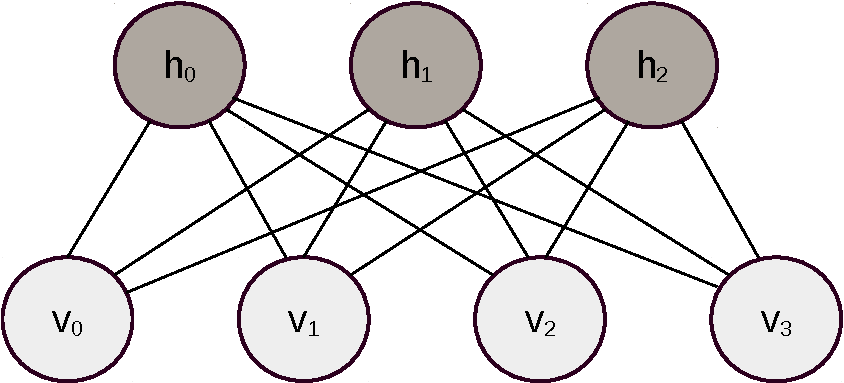
\includegraphics[width=0.6\textwidth]{pics_sdbn/RBM.pdf}
	\caption{A typical RBM structure.}
	\label{fig:RBM}
\end{figure}

The Energy function~\cite{hopfield1982neural} of a RBM is defined as follows, which has $ n $ vision units and $ m $ hidden ones:
\begin{equation}
E(\mathbf{v}, \mathbf{h} \mid \Theta)= -\sum_{i=1}^n a_i v_i - \sum_{j=1}^m b_j h_j - \sum_{i=1}^n \sum_{j=m}^n v_i W_{ij} h_j.
\end{equation}
And the model function and its probability functions are as follows:
\begin{equation}
\begin{aligned}
& f(\mathbf{v}, \mathbf{h} \mid \Theta) =e^{-E(\mathbf{v}, \mathbf{h} \mid \Theta)} \\
& p(\mathbf{v}, \mathbf{h} \mid \Theta) =\frac{e^{-E(\mathbf{v}, \mathbf{h} \mid \Theta)}}{Z(\Theta)}\\
& Z(\Theta) = \sum_{\mathbf{v}} \sum_{\mathbf{h}} e^{-E(\mathbf{v}, \mathbf{h} \mid \Theta)}.
\end{aligned}
\end{equation}
Note that, the model function $ f(\mathbf{v}, \mathbf{h} \mid \Theta) $ is nicely defined as a PoE problem, and each hidden unit represent an expert.
However, we are more interested in the marginal probability function: $ p(\mathbf{v} \mid \Theta) $:
\begin{equation}
p(\mathbf{v} \mid \Theta) =\frac{\sum_{ \mathbf{h}} e^{-E(\mathbf{v}, \mathbf{h} \mid \Theta)}}{Z(\Theta)}.
\end{equation}	

\paragraph{Objective Function}	
%\subsubsubsection{Objective Function}
Although $ p(\mathbf{v} \mid \Theta) $ is not a PoE problem, the partial derivation of the average log-likelihood function still applies to Equation~(\ref{equ:part}) and the intractable integration is the same problem here:
\begin{equation}
\label{equ:RBM}
\begin{aligned}
\dfrac{\partial \hat{l} (\Theta \mid \mathbf{D})}{\partial \theta} 
& = \left \langle \dfrac{\partial -E(\mathbf{v}, \mathbf{h} \mid \Theta)}{\partial \theta} \right \rangle_{\mathbf{h} \sim p( \mathbf{h} \mid \mathbf{v}, \Theta), \mathbf{V}} 
- \left \langle \dfrac{\partial -E(\mathbf{v}, \mathbf{h} \mid \Theta)}{\partial \theta} \right \rangle_{\mathbf{v}, \mathbf{h} \sim p( \mathbf{v}, \mathbf{h} \mid  \Theta)},  \\
\end{aligned}
\end{equation}
The detailed derivation process, please see Appendix~\ref{app:RBM}.
Regarding the specific RBM parameters,  $ \Theta = (\mathbf{a}, \mathbf{b}, \mathbf{W}) $, the derivatives are:
\begin{equation}
\label{equ:RBM_2}
\begin{aligned}
\dfrac{\partial \hat{l} (\Theta \mid \mathbf{D})}{\partial W_{ij}} 
& = \left \langle v_i h_j \right \rangle_{\mathbf{h} \sim p( \mathbf{h} \mid \mathbf{v}, \Theta), \mathbf{V}} 
- \left \langle  v_i h_j \right \rangle_{\mathbf{v}, \mathbf{h} \sim p( \mathbf{v}, \mathbf{h} \mid  \Theta)},  \\
\dfrac{\partial \hat{l} (\Theta \mid \mathbf{D})}{\partial a_{i}} 
& = \left \langle v_i \right \rangle_{\mathbf{h} \sim p( \mathbf{h} \mid \mathbf{v}, \Theta), \mathbf{V}} 
- \left \langle  v_i \right \rangle_{\mathbf{v}, \mathbf{h} \sim p( \mathbf{v}, \mathbf{h} \mid  \Theta)},  \\
\dfrac{\partial \hat{l} (\Theta \mid \mathbf{D})}{\partial b_{j}} 
& = \left \langle h_j \right \rangle_{\mathbf{h} \sim p( \mathbf{h} \mid \mathbf{v}, \Theta), \mathbf{V}} 
- \left \langle  h_j \right \rangle_{\mathbf{v}, \mathbf{h} \sim p( \mathbf{v}, \mathbf{h} \mid  \Theta)},  \\
\end{aligned}
\end{equation}
\paragraph{CD with 1-step Reconstruction} 
%\subsubsubsection{CD with 1-step Reconstruction}
\label{sec:cd}
Both terms of the derivatives of the average log-likelihood function (Equation~(\ref{equ:RBM})) are intractable, so generative models for sampling is needed.
As stated in Section~\ref{sec:CD}, for each iteration only one sample is generated.

Regarding to the first term, given a training data $ \mathbf{v}_0 $ we first generate a hidden vector according to the conditional distribution $ \mathbf{h}_0 \sim p( \mathbf{h} \mid \mathbf{v}_0, \Theta) $.
Welling et al. have proposed~\cite{welling2004exponential} that both the hidden and visible units can be any exponential unit, such as softmax, Gaussian and Poissonian.
Here we take a Bernoulli-Bernoulli RBM as an example, where each node is a sigmoidal unit.
The conditional probability function is as follows:
\begin{equation}
p(h_i = 1 \mid \mathbf{v}) = \sigma(\sum_{j=1}^{m} W_{ij} \cdot \mathbf{v} + b_j).
\end{equation}

\begin{figure}[hbt]
	\centering
	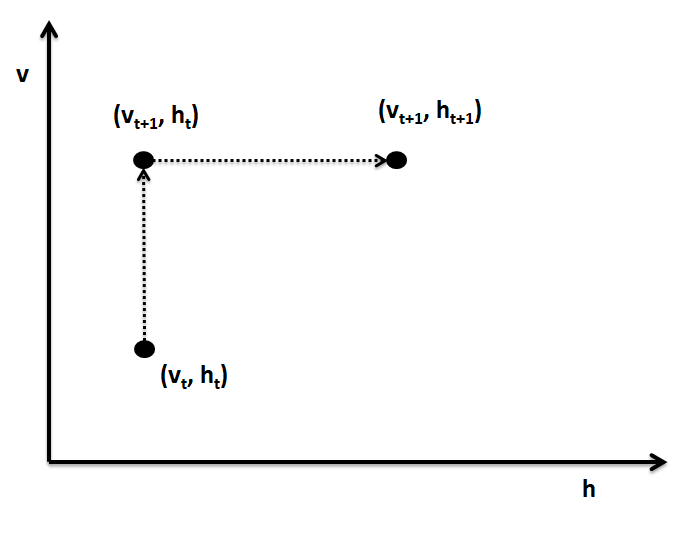
\includegraphics[width=0.6\textwidth]{pics_sdbn/gibbs.png}
	\caption{Gibbs sampling on RBM.}
	\label{fig:gibbs}
\end{figure}
The second term is perfect fit for Gibbs sampling, since we can $ p(\mathbf{v}, \mathbf{h} \mid \Theta) $ as a 2D vector and generating the samples by jumping in a Markov Chain with the transformation probability matrix $ p(\mathbf{v} \mid \mathbf{h}, \Theta) $ and $ p(\mathbf{h} \mid \mathbf{v}, \Theta) $, see Figure~\ref{fig:gibbs} and Section~\ref{sec:Gibbs}.
So, with the given data $ \mathbf{v}_0 $ and the sampling data $ \mathbf{h}_0 $, we have the initial data point in this Markov Chain,  ($ \mathbf{v}_0, \mathbf{h}_0$).
The transformation starts from the axis of $ \mathbf{v} $, then we get $ \mathbf{v}_1 \sim p( \mathbf{v} \mid \mathbf{h}_0, \Theta) $.
It follows the next axis $ \mathbf{h} $, similarly we get $ \mathbf{h}_1 \sim p( \mathbf{h} \mid \mathbf{v}_1, \Theta) $.
So far we obtain the first sample along the Markov Chain, ($ \mathbf{v}_1, \mathbf{h}_1$) thus to solve the objective function with one iteration.
The algorithm is described below:   
\begin{algorithm}[h]
	\caption{Learning on RBM Parameters with $ CD_1 $}
	\label{alg:learn}
	\begin{algorithmic}
		%			\State Initialisation $\mathbf{x}_0 = [x_0(1),x_0(2),...,x_0(M)]$,  \Comment{Random initialise $\mathbf{x}_0$}
		\For{$t=1, 2, ..., K$} \Comment{K number of training data $ \mathbf{V} $, 1 data each iteration}
		%			\For{$k=1, 2, ..., M$}
		\State $ \mathbf{h}_t \sim p( \mathbf{h} \mid \mathbf{v}_t, \Theta) $
		\Comment{Generate $ \mathbf{h}_t $ given $ \mathbf{v}_t $ }
		\State $ \mathbf{v}_{t+1} \sim p( \mathbf{v} \mid \mathbf{h}_{t}, \Theta) $
		\Comment{Generate $ \mathbf{v}_{t+1} $ on v axis using Gibbs sampling }
		\State $ \mathbf{h}_{t+1} \sim p( \mathbf{h} \mid \mathbf{v}_{t+1}, \Theta) $
		\Comment{Generate $ \mathbf{h}_{t+1} $ on h axis using Gibbs sampling }
		\State $ \dfrac{\partial \hat{l} (\Theta \mid \mathbf{D})}{\partial W_{ij}} = v_{t,i} h_{t,j} - v_{t+1,i} h_{t+1,j}$
		\State $ \dfrac{\partial \hat{l} (\Theta \mid \mathbf{D})}{\partial a_{i}} = v_{t,i} - v_{t+1,i} $
		\State $  \dfrac{\partial \hat{l} (\Theta \mid \mathbf{D})}{\partial b_{j}} = h_{t,j} - h_{t+1,j}$
		\State $ \Delta W_{ij} = \eta ( v_{t,i} h_{t,j} - v_{t+1,i} h_{t+1,j}) $
		\Comment{Update $ W_{ij} $}
		\State $ \Delta a_{i} = \eta ( v_{t,i} - v_{t+1,i}) $
		\Comment{Update $ a_{i} $}
		\State $ \Delta b_{j} = \eta ( h_{t,j} - h_{t+1,j}) $
		\Comment{Update $ b_{j} $}
		%			\EndFor
		\EndFor
	\end{algorithmic}
\end{algorithm}


\subsubsection{noisy RBM}
Instead of using binary units in RBM, we employ noisy ReLU units constructing noisy RBM which is closer to biology and performances better in classification tasks\cite{nair2010rectified}.

%	\chapter{Deep Learning}
\label{cha:dnn}
Deep Learning research in the field of Artificial Neural Networks~(ANNs) has dominated state-of-the-art solutions on cognitive tasks, e.g. the performance exceeding human-level  on image classification tasks~\citep{he2015delving} and playing GO~\citep{silver2016mastering}.
Merging Deep Learning techniques into Spiking Neural Networks~(SNNs), introduced in the previous chapter, may provide an answer to the problem of how to operate SNNs to perform equivalently as ANNs in cognitive tasks. 
In this chapter, we will give an overview of popular architectures and models of Deep Learning in Section~\ref{sec:dl_history}, and the rest of this chapter will illustrate the mechanisms of Convolutional Networks (ConvNets), Autoencoders (AEs), and Restricted Boltzmann Machines~(RBMs) in detail which will be used in following chapters.

\section{Brief Overview}
\label{sec:dl_history}
Deep Learning seems to have become the answer to all artificial intelligence problems overnight since Geoffrey Hinton proposed the training method of a type of ANN, the Deep Belief Network, in 2006~\citep{hinton2006fast}.
However, Deep Learning is not a new `magic', but rather has a history over a few decades and its sudden success is the result of the availability of an increasing amount of training data, the growing size of network models and greater computational power.
Therefore, all the classical Deep Learning architectures date back to the last century before the `Deep Learning' name was coined.
However, at that time, deep networks could hardly be trained, mainly because of the limits on computational power.


\subsection{Classical Models}
We call the well-known and widely-used Deep Learning models `classical' and give a brief introduction to those models in this section. 
As mentioned above, the first break-through in training deep, as opposed to shallow ($\le 3$ layers), networks was the greedy layer-wise strategy~\citep{hinton2006fast} proposed to train stacked RBMs, which will be described in more detail in Section~\ref{sec:rbm}.
Shortly after, this method was proved also to be efficient for training other kinds of deep networks including stacked AEs~\citep{bengio2007greedy} (stated in Section~\ref{sec:AE}).
RBMs and AEs are suitable for dimensionality reduction and feature extraction when trained with unsupervised learning on unlabelled data.
In 2012, using such an unsupervised Deep Learning architecture, the Google Brain team achieved a milestone in the Deep Learning era; the neural network learned to recognise cats by `watching' 10 million images generated from random frames of YouTube videos~\citep{le2013building}.

ConvNets are biologically inspired from the significant discovery of Hubel and Wiesel that the orientation selectivity (simple cells) and pooling mechanism (complex cells) represent the basic functions in the primary visual cortex in cats~\citep{hubel1962receptive}.
These simple cells fire at a high frequency to their preferred orientation of visual stimuli within their receptive fields~(shown in Figure~\ref{Fig:v1}), small sub-regions of the visual field.
%This means a single simple cell works like a pattern detector within its small receptive field thus also providing the exact spatial location of the detected feature in the entire visual field.
Meanwhile, a complex cell corresponds to the existence of a pattern within a larger receptive field but loses the exact position of the pattern.
%This means that its receptive field cannot be mapped into fixed excitatory and inhibitory zones. Rather, it will respond to patterns of light in a certain orientation within a large receptive field, regardless of the exact location.
%The receptive fields composes of the entire visual field.
%These cells act as local filters over the input space and are well-suited to exploit the strong spatially local correlation present in natural images.
The NeoCognitron~\citep{fukushima1982neocognitron} was the first network to mimic the functions of V1 simple and complex neurons in an ANN, and later this feature detection of single cells was improved by sharing weights among receptive fields in LeNet-5~\citep{lecun1998gradient}, the typical ConvNet used today.
The mechanism of shared weights forms the essence of convolution in a ConvNet, which hugely reduces the number of weight parameters in a network.
The most significant milestones produced by deep ConvNet dominated the best performances in the annual ImageNet Challenge~\citep{russakovsky2015imagenet}: AlexNet~\citep{krizhevsky2012imagenet}, VGG Net~\citep{simonyan2014very}, GoogLeNet~\citep{szegedy2015going} and ResNet~\citep{he2016deep}.

Despite the powerful capabilities of these feed-forward deep networks, sequence processing is a challenge for them since the size of the input and output vectors are constrained to the number of neurons.
Thus Recurrent Neural Networks~(RNNs), containing feed-back connections, are ideal solutions for dealing with sequential information since their current output is always dependent on the previous `memory'.
As training mechanisms have become more mature, for example using the Long Short-Term Memory~(LSTM)~\citep{hochreiter1997long}, RNNs have shown great success in many natural language processing tasks: language modelling~\citep{mikolov2010recurrent}, machine translation~\citep{sutskever2014sequence}, speech recognition~\citep{graves2014towards} and image caption generation~\citep{karpathy2015deep}.

\subsection{Combined Approaches}
The current trend in Deep Learning is to combine machine learning algorithms towards more complex objectives such as decision making and data generation.

Reinforcement Learning (RL) is inspired from animal behaviour when agents learn to make sequential optimised decisions to control an environment.
To address complex decision making problems in practical life, RL requires a sufficiently abstract representation of the high-dimensional environment.
Fortunately, Deep Learning just complements the requirement which performs effectively at dimensionality reduction and feature extraction.
The milestone achieved by the integration of RL and deep networks, deep RL, drew everyone's attention to artificial intelligence when AlphaGo beat a professional human player at Go~\citep{silver2016mastering}.
%which has been successfully applied to various tasks: such as games~\citep{mnih2015human}, robotics~\citep{schulman2015trust} and question-and-answer systems.
%Potential in real-time neuromorphic system
%These real-time decision making systems, especially used for robotics~\citep{schulman2015trust}, are ideal for meromorphic hardware systems which takes advantages in event-based processing and energy efficiency.
%http://blog.aylien.com/introduction-generative-adversarial-networks-code-tensorflow/

Generative Adversarial Networks (GANs)~~\citep{goodfellow2014generative} are proposed for training generative models of complex data.
Instead of training discrimination networks (e.g. image classification using CovNets ) and generation networks (e.g. data sampling on RBMs) separately with different objectives, GANs train two competing networks, one the discriminator, the other the generator, simultaneously by continuously making them play games with each other.
Thus, the generator learns to produce more realistic data to fool the discriminator; meanwhile the discriminator learns to become better at distinguishing generated from real data.
Exciting achievements have been reported in generating complex data such as realistic image generation based on descriptions in text~\citep{radford2015unsupervised}.

\section{Convolutional Networks}
\label{sec:convnet}
In Chapter~\ref{cha:Conv}, we will use a convolutional network to demonstrate a training method for spiking deep architectures.
This section aims to give a detailed introduction to ConvNet architectures and their training with Backpropagation.
\subsection{Network Architecture}

	\begin{figure}[bt]
		\centering
		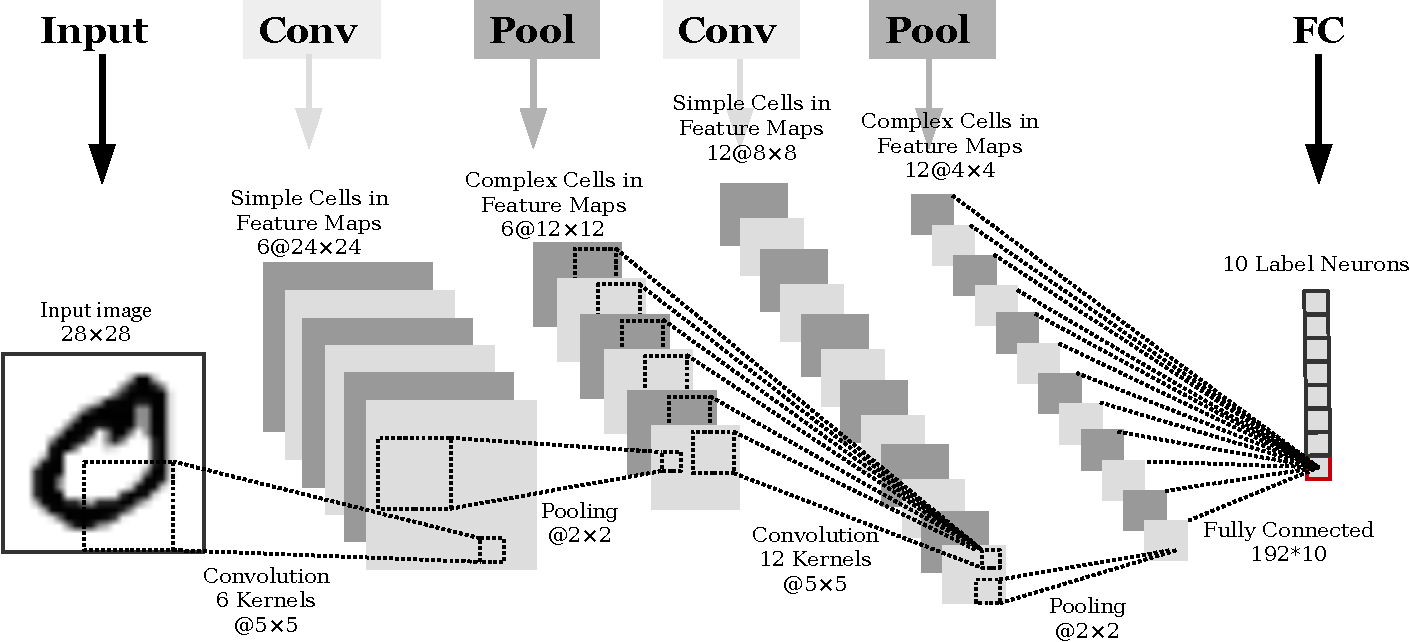
\includegraphics[width=0.95\textwidth]{pics_snn/convnet.pdf}
		\caption{Typical ConvNet architecture.}
		\label{Fig:ConvNet}
	\end{figure}

A typical ConvNet, LeNet shown in Figure~\ref{Fig:ConvNet},  consists of four types of neural layers: an input layer, convolutional~(Conv) layers of simple cells, pooling~(Pool) layers of complex cells and fully-connected~(FC) layers.
From the left to right of Figure~\ref{Fig:ConvNet}, we illustrate the mechanism of the ConvNet in detail.

The pixels of the input image are normalised and fed into the first Conv layer.
Every simple cell takes inputs within its receptive field and the weights on each input pixel are determined by the convolutional kernel which has the same size as the receptive field.
The neurons work as demonstrated in Figure~\ref{Fig:compare_as}(a) performing a dot product between the weights and the input volume of a receptive field; this is followed by an activation function.
Convolving a whole input image with a kernel composes a feature map in the Conv layer, thus in this LeNet example there are 6 feature maps in the first Conv layer.
Stride controls the output volume of a convolution such that setting the stride to $step$ causes the kernel to move $step$ pixels at a time.
Thus a small stride produces more output volume and highly overlapping receptive fields.
Suppose an input image and a kernel are both squares, with side lengths of $l_{in}$ and $l_k$, then the side length of the convolved feature map is $(l_{in} - l_k + 1)/stride$.

The special characteristics of Conv layers lie in the local connectivity and the parameter sharing, such that a neuron connects only to a spatially local input volume, its receptive field; and the weights (the convolutional kernel) are shared among all the receptive fields.
Consequently, the number of parameters (trainable weights) hugely decreases compared to all-to-all connections of the same network size. 

The complex neurons of the Pool layers either output the maximum input within their receptive fields (max pooling) or the average (average pooling), by applying a max/average filter to non-overlapping receptive fields.
The pooling process reduces the spatial size of the feature maps but keeps the number of features.
In Chapter~\ref{cha:Conv}, we will use average pooling of $2\times2$ for all the Pool layers, as shown in Figure~\ref{Fig:ConvNet}.
The average filter traverses an entire feature map with a stride of 2, and outputs the averaged element of each receptive field to the next layer.

The next Conv layer drives 3D feature vectors with a depth of 6 (six feature maps) to convolve with 12 3D kernels with size of $6\times5\times5$.
The example demonstrates a common set-up using all the feature maps of the 3D feature vectors; usually it is feasible to select a subset of the input feature maps to involve in the convolutions with each kernel.
Then a Pool layer follows the convolution.
Repeating these alternating presentations of a Conv layer and a Pool layer builds up a deeper ConvNet.

The trainable shared weights used in the Conv layer hugely reduce the number of weight parameters in a ConvNet, while Pool layers use static convolutional kernels to shrink the size of the network.
These convolutional connections can be described as 6c5-2s-12c5-2s, where $\alpha c \beta$ indicates $\alpha$ kernels of side length $\beta$ used in the Conv layer, and $2s$ specifies the side length and the stride of a pooling kernel.
However, a Multilayer Perceptron (MLP) network possesses only FC layers, where each neural layer fully connects to the next one.
In a ConvNet an FC layer is usually located at the last layer (right in Figure~\ref{Fig:ConvNet}), and connects the last Pool layer to the output neurons with all-to-all connections.
% to predict the classification of the input image.
The strongest response among the output neurons indicates to which class the input image belongs, as illustrated in Figure~\ref{Fig:ConvNet} where the red neuron represents the first digit out of ten, `0'.
There can be more than one FC layer at the end of a ConvNet.
In this thesis, we will use only a single FC layer.


%Chain rule, reduced parameter amounts. 

\subsection{Backpropagation}
We have described the feed-forward path of a ConvNet to classify an input image.
In this section we will demonstrate the training of a network by back-propagating errors to tune the connection weights.
The objective function (or loss function) estimates an error by comparing the output vector of a network, $\mathbf{y}=(y_1,y_2,...,y_M)$, to the desired label vector, $\mathbf{t}=(t_1,t_2,...,t_M)$, and the error is to be minimised during training.
Given a set of training data with desired labels $\mathbf{T}=\{\mathbf{t}^1, \mathbf{t}^2, ..., \mathbf{t}^K\}$ and the network output $\mathbf{Y}=\{\mathbf{y}^1, \mathbf{y}^2, ..., \mathbf{y}^K\}$ the Mean Squared Error~(MSE) can be seen as the objective function:  
\begin{equation}
L={MSE}(\mathbf{T}, \mathbf{Y}) =\frac{1}{2K}\sum_{k=1}^K \sum_{m=1}^M (y^{k}_{m}-t^{k}_{m})^{2}~~.
\label{equ:loss_all}
\end{equation}

BP propagates the gradient of the loss with respect to the weights backwards to each connection in the network.
The computation requires a closer look into the structure of a neuron, see Figure~\ref{Fig:neuron_net} where $N$ neurons connect to the $j^{th}$ neuron of the next layer, and the neuron converts the weighted summation of the input, $net_j$, to the output $y_j$ according to its activation function.
\begin{figure}[bt]
	\centering
	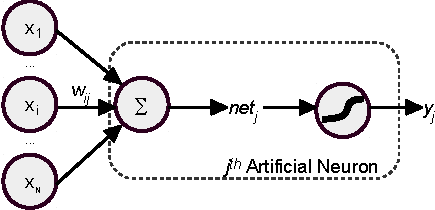
\includegraphics[width=0.7\textwidth]{pics_iconip/neuron.pdf}
	\caption[An artificial neuron.]{$N$ neurons connect to the $j_{th}$ neuron of the next layer. As illustrated in Figure~\ref{Fig:compare_as}(a), we use a simplified artificial neuron without bias.}
	\label{Fig:neuron_net}
\end{figure}

Thus the gradient of the loss $L$ with respect to a weight $w_{ij}$ is as follows:
\begin{equation}
\begin{aligned}
\frac{\partial L}{\partial w_{ij}} &= \frac{\partial L}{\partial y_j} \frac{\partial y_j}{\partial net_j} \frac{\partial net_j}{\partial w_{ij}} = \delta_j x_i , \textrm{~~where~~}\\
 \delta_j &=  \frac{\partial L}{\partial y_j} \frac{\partial y_j}{\partial net_j}~~,  \textrm{~~and~~}\\
% \frac{\partial y_j}{\partial net_j} &= f'(net_j)~~, \\
x_i &= \frac{\partial net_j}{\partial w_{ij}}~~.
\end{aligned}
\end{equation}
The term $ \delta_j $ represents the error gradient with respect to $net_j$, and can be expressed by a recursive definition:
\begin{equation}
\begin{aligned}
\delta_j =  \frac{\partial L}{\partial y_j} \frac{\partial y_j}{\partial net_j} &= \left\{
\begin{aligned}
&\frac{1}{K}\sum_{k=1}^K (y^{k}_{j}-t^{k}_{j}) f'(net_j)  \textrm{~,~~if \textit{j} is in an output layer} \\
&(\sum_l^L \delta_l w_{lj}) f'(net_j)  \textrm{~,~~otherwise}
\end{aligned}
\right. \\
\textrm{,~~where~~} \frac{\partial y_j}{\partial net_j} &=  f'(net_j) \textrm{~,~~the derivative of the activation function}.
\end{aligned}
\label{equ:derivative}
\end{equation}
It is easy to obtain the first term, $ \frac{\partial L}{\partial y_j}  $, of $ \delta_j $ when $j$ is an output neuron, since it only involves a single dimension of the output vector.
However, when $j$ is in an inner layer of the network, which connects to $L$ neurons on the next layer, we have to take the total derivative with respect to $y_j$: $\sum_l^L \delta_l w_{jl}$.
The error propagation applies to any form of connection in a network, such as FC and Conv layers, and the difference only appears in the summation where the matrix product is used for the FC layer and convolution for the Conv layer.
In addition, the weights used in BP are either transposed in the FC layer or rotated in the Conv layer compared to the forward path.

After error propagation, the BP algorithm updates weights using the optimisation method, gradient descent, to minimize the objective function.
It modifies the weights by small steps proportional to the negative of the gradients:
\begin{equation}
\Delta w_{ij} \propto -\frac{\partial L}{\partial w_{ij}} = -\eta \delta_j x_i~~,
\label{equ:delta_w}
\end{equation}
where $\eta$ defines the length of these updating steps which is also called the learning rate.
Again, the weight update is also dependent on the types of layer, where a convolution of the input vector $\mathbf{x}$ with the error gradient  $\mathbf{\delta}$ is needed in Conv layers.
A detailed description of BP training on ConvNets can be found elsewhere~\citep{bouvrie2006notes}.

Moreover, applying Stochastic Gradient Descent (SGD), the gradient over the full training set can be approximated using only a few, even a single, training data.
Therefore $k$ in Equation~\ref{equ:derivative} can be seen as a randomly selected data index, and $K$ represents the number of elements in such a data subset, which is also known as a batch.
If we take only one data sample in each batch, the loss function~(Equation~\ref{equ:loss_all}) will be estimated by the error between an output vector $\mathbf{y}^k$ and the single label sample $\mathbf{t}^k$:
\begin{equation}
E^k = \frac{1}{2}\sum_{m=1}^M (y^{k}_{m}-t^{k}_{m})^{2}~~,
\label{equ:error_conv}
\end{equation}
and the equation can be simplified by deleting the index $k$, assuming the error is computed for each data sample:
\begin{equation}
E = \frac{1}{2}\sum_{m=1}^M (y_{m}-t_{m})^{2}~~.
\label{equ:error_non}
\end{equation}


\subsection{Activation Function and Vanishing Gradient}

%\begin{figure}[hbt]
%	\centering
%	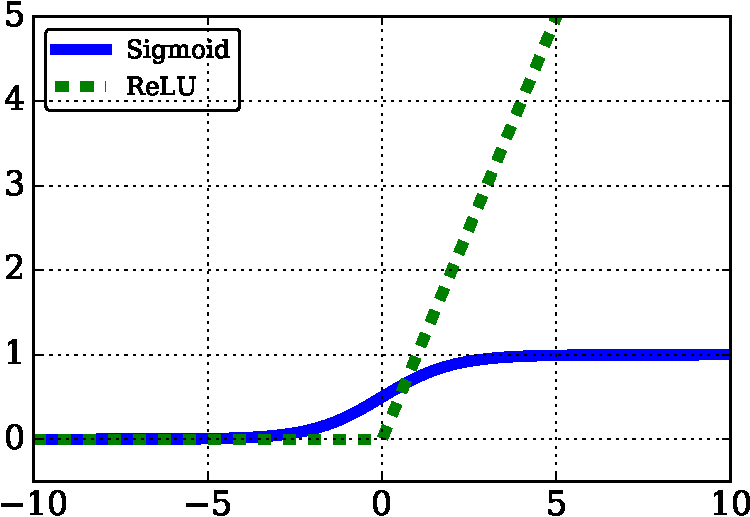
\includegraphics[width=0.6\textwidth]{pics_snn/af.pdf}
%	\caption{Activation functions: sigmoid and ReLU.}
%	\label{fig:af}
%\end{figure}

\begin{figure}[tbp!]
	\centering
	\begin{subfigure}[t]{0.48\textwidth}
		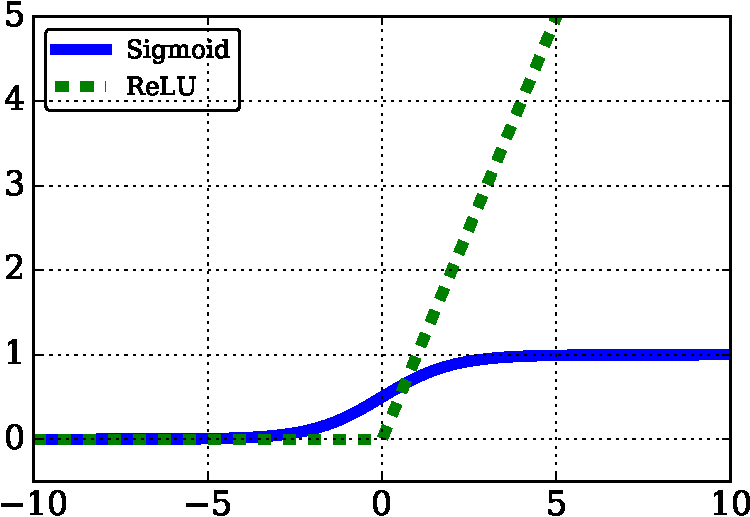
\includegraphics[width=\textwidth]{pics_snn/af.pdf}
		\caption{Activation functions}
	\end{subfigure}
	~~
	\begin{subfigure}[t]{0.48\textwidth}
		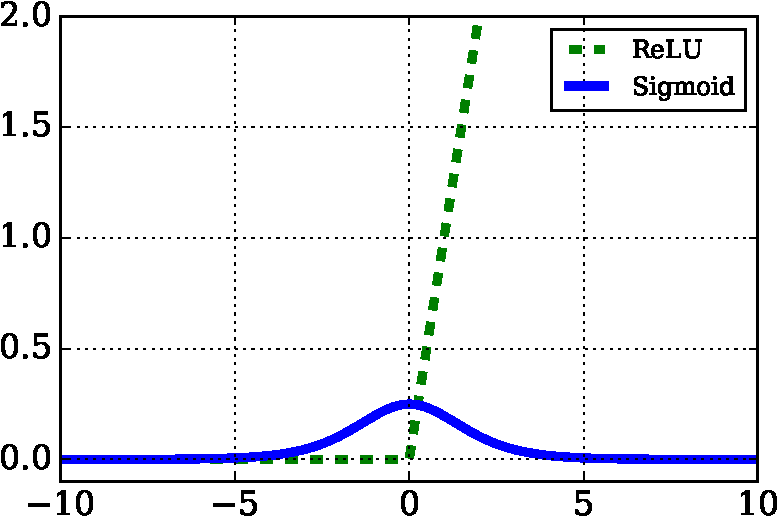
\includegraphics[width=\textwidth]{pics_snn/af_der.pdf}
		\caption{Derivatives of the activation functions}
	\end{subfigure}
	\caption[Activation functions]{Activation functions: (a) sigmoid and ReLU, and (b) their derivatives.}
	\label{fig:af}
\end{figure}
Each error gradient propagated through layers of the network consists of a chain of multiplied factors as illustrated in Equation~\ref{equ:derivative}.
The deeper a network is and the closer a layer is to the input, the more elements are involved in the multiplication including the derivative of the activation function.
%The derivative of the activation function is a recursive factor in the BP chain, 
%one of the factors when the error gradient back propagated in each layer.
Thus, the gradient may vanish if the derivative of the activation function is always less than 1.
For the sigmoid function example, shown in Figure~\ref{fig:af}(a), the derivative only peaks to around~0.25 when the input is close to 0, and decays to its minimum as the input either increases or decreases, see Figure~\ref{fig:af}(b).

The Rectified Linear Unit (ReLU) is proposed to tackle the problem of vanishing gradients in deep networks.
ReLU, simply defined as $y = max(0,x)$ and shown in Figure~\ref{fig:af}, has a gradient of 1 when the input is greater than 0.
Hence, the error gradient is able to be back-propagated in deeper networks by multiplying ReLU derivatives.

\section{Autoencoders}
\label{sec:AE}
Autoencoders~(AE) are categorised as unsupervised learning systems, since AE aims to reconstruct its original input as closely as possible.
Thus the output and input vectors have the same dimensionality, but the hidden middle layer is allowed to have either more, or fewer, neurons for the purpose of compressing the inputs or mapping them to higher dimensions.
Hence the AE is suitable for learning an effective representation of the original inputs at the hidden layer, which can be seen as the encoding phase of the AE, and reconstructing them on the output layer where the hidden vectors are decoded. 

Multiple AEs can be stacked to build deep AEs where the hidden layer of a lower AE represents the input of the upper block, and each AE block can be trained individually with greedy layer-wise training~\citep{hinton2006fast}.
A stacked AE takes advantage of greater expressive power as does any deep network.
Taking image processing as an example, the lower AE blocks learn only simple features, such as edges and dots, however on the upper layers more complicated and abstract features are extracted: contours, symbols and even objects. 

In this section, we will only describe the structure and training method of single AE blocks, since the greedy layer-wise training on stacked AEs is no different from training multiple single AEs except for different input data.
Due to the AE's simple network architecture and training algorithm, spiking AEs will be built and trained with a biologically-plausible training mechanism in Chapter~\ref{cha:sdlm}.

\subsection{Structure}
Figure~\ref{fig:AE} shows the architecture of an AE, which is an MLP consisting of three layers of neurons: the visible ($\mathbf{v}$), hidden ($\mathbf{h}$) and reconstruction ($\mathbf{v'}$) layers.
Both visible and reconstruction layers have $N$ dimensions, and the hidden layer has $M$.
Note that AEs usually have tied weights where the connections ($\mathbf{w}^T$) between $\mathbf{v}$ and $\mathbf{h}$ are transposed to form the connections ($\mathbf{w}$) from $\mathbf{h}$ to $\mathbf{v'}$.


\begin{figure}
	\centering
	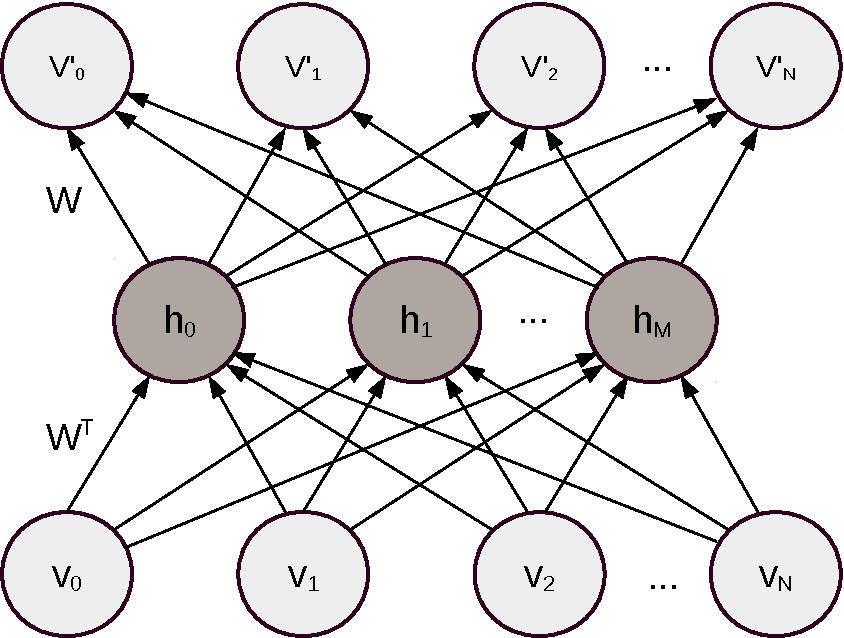
\includegraphics[width=0.5\textwidth]{pics_sdlm/AE.pdf}
	\caption{A typical Autoencoder structure.}
	\label{fig:AE}
\end{figure}


\subsection{Training}
The feedforward path of an AE, as for an MLP, non-linearly transforms the input through two FC layers, where each neuron performs weighted summation and activation as illustrated in Figure~\ref{Fig:neuron_net}.
Training an AE is also similar to that for an MLP, however, the difference lies in the objective where the AE aims to minimise the difference between the input $\mathbf{v}$ and its reconstruction $\mathbf{v'}$, instead of between the output and some labelled data (supervised learning).
Therefore the loss function generated by a single data sample $\mathbf{v}$, described in Equation~\ref{equ:error_non} for supervised learning, is as follow:
\begin{equation}
E = \frac{1}{2}\sum_{n=1}^N (v'_{n}-v_{n})^{2}~~,
\end{equation}
and the weight update, shown in Equation~\ref{equ:delta_w}, is proportional to the error gradient with respect to the weight:
\begin{equation}
\Delta w_{ij} \propto -\frac{\partial E}{\partial w_{ij}} = -\eta \delta_j h_i~~,
\end{equation}
where $\eta$ is the learning rate, $h_i$ is the hidden neuron and the term $\delta_j$ is the error gradient with the respect to $net_j$, the weighted summation.
The weight tuning needs only to be applied in the reconstruction layer, since study~\citep{xu1993least} has proved that updating the transposed weights $\mathbf{w}^T$ at the hidden layer does not improve the learning and the error gradients are usually small.
Hence, $\delta_j$  can be calculated according to Equation~\ref{equ:derivative}:
\begin{equation}
\delta_j = (v'_{j}-v_{j}) f'(net_j)~~,
\end{equation}
and the weight update can be simply described by:
\begin{equation}
\Delta w_{ij} = \eta h_i (v_{j}-v'_{j})  f'(net_j)~~.
\end{equation}
If we use ReLU as the activation function, then the above equation is as follow:
\begin{equation}
\label{equ:ae_widrow_hoff}
\Delta w_{ij} = \left \{
\begin{aligned}
& \eta h_i(v_j - v'_j)~, & net_j > 0 \\
& 0~, & net_j < = 0
\end{aligned} 
\right.
\end{equation}

%\begin{equation}
%\begin{aligned}
%\Delta w_{ij} = -\eta \frac{\partial E_k}{\partial w_{ij}} &= -\eta \frac{\partial E_k}{\partial v'_j} \frac{\partial v'_j}{\partial net\_v'_j} \frac{\partial net\_v'_j}{\partial w_{ij}}, \textrm{ where} \\
%\frac{\partial E_k}{\partial v'_j} &= \frac{\partial \frac{1}{2} \sum_l (v_l - {v'}_l)^2}{\partial v'_j}= \frac{\partial \frac{1}{2}(v_j - {v'}_j)^2}{\partial v'_j}= v'_j - v_j, \\
%%	\frac{\partial v'_j}{\partial net\_v'_j} &= \begin{cases} 1, v'_j>0\\0, v'_j<=0\\ \end{cases}, \textrm{using ReLU,}\\
%%\frac{\partial v'_j}{\partial net\_v'_j} &=\left\{
%%\begin{aligned}
%%& 1, net\_v'_j > 0 \\
%%& 0, net\_v'_j < = 0
%%\end{aligned} 
%%\right.    \textrm{using ReLU, }\\
%\frac{\partial v'_j}{\partial net\_v'_j} &= f'(net\_{v'_j})~, \textrm{~derivative of the activation function} \\
%\frac{\partial net\_v'_j}{\partial w_{ij}} &= \frac{\partial h_i w_{ij}}{\partial w_{ij}} = h_i.
%\end{aligned}
%\end{equation}
%Thus, the weight gradient is calculated as:
%\begin{equation}
%\label{equ:ae_widrow_hoff}
%%\Delta w_{ij} = \left \{
%%\begin{aligned}
%%& \eta h_i(v_j - v'_j), &net\_v'_j > 0 \\
%%& 0, & net\_v'_j < = 0
%%\end{aligned} 
%%\right.
%\Delta w_{ij} = \eta h_i f'(net\_{v'_j}) (v_j - v'_j)~~.
%\end{equation}

%\section{Restricted Boltzmann Machine}
%\label{sec:rbm}
%In order to implement training and testing of Spiking Deep~Belief~Networks~(SDBNs) on-line, this section studied:
%\begin{itemize}
%	\item \textit{Contrastive Divergence.}
%	The study starts from understanding the original problem, Products of Experts~(PoE), which was solved by using Contrastive~Divergence~(CD).
%	It involves utilising Markov~Chain~Monte~Carlo~(MCMC) sampling to present the distribution of a certain untraceable high-dimensional probability model function, e.g. PoE.
%	Among these sampling algorithms, Gibbs method is introduced and used in high dimensional problems.
%	Instead of minimising the original objective function of Kullback-Leibler divergence, the contrastive divergence is exploited to solve PoE.
%	\item \textit{Restricted Boltzmann Machine (RBM). }
%	Then the study continues on applying Gibbs sampling and CD to RBM, which builds the foundation of the light RBM training.
%	\item \textit{Deep Belief Network.} 
%	The greedy algorithm on training layered RBMs and the fine training on the whole DBN are studied.
%\end{itemize}
%Next, the study will carry on to on-line learning methods which only applies to spiking neurons for training spiking RBM and DBN.
%\subsection{Contrastive Divergence\citep{hinton2002training,woodfordnotes}}
%The probability of a vector point $ \mathbf{x} $ is modelled by the function $f(\mathbf{x} \mid \Theta )$ given the model parameters $ \Theta $, and normalised by a partition function $Z( \Theta)$:
%
%\begin{equation}
%p(\mathbf{x} \mid \Theta ) = \dfrac{f(\mathbf{x} \mid \Theta )}{Z( \Theta)}
%\end{equation}
%where the partition function is defined as:
%\begin{equation}
%\label{equ:z_int}
%Z( \Theta) = \int f(\mathbf{x} \mid \Theta )\D\mathbf{x}, \text{when  $ \mathbf{x} $ is continuous, or}
%\end{equation}
%
%\begin{equation}
%\label{equ:z_dis}
%Z( \Theta) = \sum_{\mathbf{x}} f(\mathbf{x} \mid \Theta ), \text{when  $ \mathbf{x} $ is discrete.}
%\end{equation}
%Given a set of data points $ \mathbf{D}=(\mathbf{d}_1, \mathbf{d}_2, ..., \mathbf{d}_K) $ the purpose of learning is to tune the model parameter $ \Theta $ to fit the data $ \mathbf{D}  $. 
%The objective function is the probability product of all the independent data points of the data set, which is also called the likelihood function:
%\begin{equation}
%L (\Theta \mid \mathbf{D}) = p(\mathbf{D} \mid \Theta ) = \prod_{k=1}^K p(\mathbf{d}_k \mid \Theta ) =  \prod_{k=1}^K\dfrac{f(\mathbf{d}_k \mid \Theta )}{Z( \Theta)}.
%\end{equation}
%And the target is to maximise the likelihood given the data set $ \mathbf{D}  $, which equals to maximise the log of the probability product (the log-likelihood):
%\begin{equation}
%\log  L (\Theta \mid \mathbf{D}) = \log p(\mathbf{D} \mid \Theta ) = \sum_{k=1}^K\log f(\mathbf{d}_k \mid \Theta ) - K \log Z( \Theta),
%\end{equation}
%or the average log-likelihood:
%\begin{equation}
%\label{equ:like}
%\hat{l} (\Theta \mid \mathbf{D}) =\frac{1}{K}\log  L (\Theta \mid \mathbf{D}) 
%=\frac{1}{K}\sum_{k=1}^K\log f(\mathbf{d}_k \mid \Theta ) - \log Z( \Theta).
%\end{equation}
%Imagine three different conditions (probability function) as following.
%
%\textbf{First}, $f(\mathbf{x} \mid \Theta )$ is the probability density function (pdf) of a normal distribution $\mathcal{N}(x \mid \mu, \sigma )$.
%Data vector $ \mathbf{x} $ is just a one dimensional data point, $x$.
%$ Z( \Theta) $ equals to 1, thus $p(x \mid \Theta ) = \mathcal{N}(x \mid \mu, \sigma )$.
%\begin{equation}
%\hat{l} (\Theta \mid D) =  
%\frac{1}{K} \sum_{k=1}^K \log \left[ \frac{1}{\sigma \sqrt{2\pi}} \exp(-\frac{(d_k-\mu)^{2}}{2\sigma^{2}}) \right]
%\label{pdf}
%\end{equation}
%To maximise Equation~\ref{pdf} is to find the Maximum Likelihood Estimation (MLE) of parameters $ \mu $ and $ \sigma $, by deriving from the partial differential equations when they are equal to 0. 
%\begin{equation}
%\left\{
%\begin{aligned}
%&\dfrac{\partial \hat{l} (\Theta \mid D)}{\partial \mu}= \sum_{k=1}^K -\frac{1}{2\sigma^{2}}\dfrac{\partial (\mu-d_k)^{2}}{\partial \mu} = \sum_{k=1}^K -\frac{1}{\sigma^{2}}(\mu-d_k) = 0 \quad\\
%&\dfrac{\partial \hat{l} (\Theta \mid D) }{\partial \sigma^{2}}= -\frac{K}{2\sigma^{2}}+\frac{1}{2\sigma^{4}}\sum_{k=1}^K d_k^{2} -\frac{\mu}{\sigma^{4}}\sum_{k=1}^K d_k + \frac{K\mu^{2}}{2\sigma^{4}} = 0 \quad\\
%\end{aligned}
%\right.
%\end{equation}
%\begin{equation}
%\left\{
%\begin{aligned}
%&\mu= \frac{1}{K}\sum_{k=1}^K d_k  \quad\\
%&\sigma^{2} = \frac{1}{K}\sum_{k=1}^K d_k^{2} - (\frac{1}{K}\sum_{k=1}^K d_k)^{2}
%\end{aligned}
%\right.
%\end{equation}
%$\hat{l} (\Theta \mid D)$ here is the function of two dimensional parameters $\mu$ and $\theta$, and searching the highest point in the parameter space ``is equivalent to being in the field on a clear, sunny day,''~\citep{woodfordnotes} seeing the point straight away.
%
%\textbf{Second}, the probability model function changes to be the sum of N normal distributions: 
%\begin{equation}
%f(x \mid \Theta ) = \sum_{i=1}^N\mathcal{N}(x \mid \mu_i, \sigma_i ).
%\end{equation}
%Derived from Equation~(\ref{equ:like}), the objective function is:
%\begin{equation}
%\hat{l} (\Theta \mid D) = \frac{1}{K}\sum_{k=1}^K \log \sum_{i=1}^N \mathcal{N}(d_k \mid \mu_i, \sigma_i ) - \log N,
%\end{equation}
%where $\log Z( \Theta)$ still equals a constant, but the partial differential equation of any parameter depends on other model parameters.
%It is very hard to solve equation set of log of sum, thus iteration methods are introduced, e.g., gradient descent method. %and expectation maximization (EM) algorithm
%Searching for a local maximum of the likelihood function in the parameter space starts with an initial point, either random or well selected.
%For each iteration, the partial derivatives for every dimension of the parameter point are calculated as the gradient.
%The gradient determines the decent direction of the space search, the next parameter point is one step $ \eta $  towards the direction or is the highest point found by line search.
%
%The gradient descent method is equivalent to ``being in the field at night with a torch.''~\citep{woodfordnotes}.
%And then the descent direction is estimated and chosen by using the torch to see the relative heights of the field a short distance in each direction.
%Because partial differential equation of any parameter depends on other model parameters, we can only see the gradient for a small area.
%The search will follow the direction by walking one step or a certain distance (e.g. line search lowest point), and then start a new iteration.
%
%%\paragraph{PoE Problem} 
%\subsubsection{PoE Problem}
%\textbf{Finally}, the probability model function becomes the product of N normal distributions: 
%\begin{equation}
%f(x \mid \Theta ) = \prod_{i=1}^N\mathcal{N}(x \mid \mu_i, \sigma_i ),
%\end{equation}
%where the partition (normalisation) function $Z( \Theta)$ is no longer a constant, but varies accordance to all the parameters.
%Essentially, the integration of the probability model, see Equation~(\ref{equ:z_int}) and~(\ref{equ:z_dis}), is usually algebraically intractable.
%We have to use numerical integration method to evaluate the Equation~(\ref{equ:like}), whose partial derivative is (we are using vectors to generalise the problem):
%\begin{equation}
%\label{equ:part}
%\begin{aligned}
%\dfrac{\partial \hat{l} (\Theta \mid \mathbf{D})}{\partial \theta} 
%& = \frac{1}{K} \dfrac{\partial \sum_{k=1}^K\log f(\mathbf{d}_k \mid \Theta )}{\partial \theta} - \dfrac{\partial \log Z( \Theta)}{\partial \theta}\\
%& =  \frac{1}{K}\sum_{k=1}^K \dfrac{\partial \log f(\mathbf{d}_k \mid \Theta)}{\partial \theta} - \int p(\mathbf{x} \mid \Theta) \dfrac{\partial \log f(\mathbf{x} \mid \Theta)}{\partial \theta} \D \mathbf{x}\\
%& = \left \langle \dfrac{\partial \log f(\mathbf{d} \mid \Theta)}{\partial \theta}\right \rangle_{\mathbf{D}} -\left \langle \dfrac{\partial \log f(\mathbf{c} \mid \Theta)}{\partial \theta}\right \rangle_{\mathbf{C} \sim p(\mathbf{x} \mid \Theta)}  \\
%&=\left \langle \dfrac{\partial \log f(\mathbf{x} \mid \Theta)}{\partial \theta}\right \rangle_{\mathbf{X}_{data}} - \left \langle \dfrac{\partial \log f(\mathbf{x} \mid \Theta)}{\partial \theta}\right \rangle_{\mathbf{X}_{model}},
%\end{aligned}
%\end{equation}
%where  $ <\cdot>_x $ denotes the mean expectation of $ \cdot $ given distribution of $x$.
%The first term of the right-hand side is easy to get with the given data set $ \mathbf{D} $, and the second term can be approximated by generating data samples $ \mathbf{C} $ according to $ p(\mathbf{x} \mid \Theta) $.
%These generative samples is called ``fantasy data'' and can be generated using Monte Carlo Markov Chain (MCMC) sampling, see section~\ref{sec:mcmc}.
%The detailed derivation process can be found in Appendix~\ref{app:part}.
%Although in this example the integration of product of normal distribution is still tractable, it is also helpful to use numerical integration.
%
%Go back to the metaphor of the parameter field, solving PoE problem is like searching the highest point in a completely dark night without a torch.
%The computation of Equation~(\ref{equ:part}) is to ``feel the gradient of the field under our feet''.~\citep{woodfordnotes}.
%%The motivation underlining Contrastive Divergence algorithm is to boost the training speed of a Markov Chain in order to represent the distribution of a PoE (Product of Expert) model.
%%Thus the sampling can be followed using this trained Markov Chain model. 
%
%%\paragraph{MCMC Sampling}
%\subsubsection{MCMC Sampling}
%\label{sec:mcmc}
%In order to solve the integration of algebraically intractable equations we can use numerical integration to approximate.
%One of the popular method is Monte Carlo integration:
%\begin{equation}
%\int_{a}^{b} f(x) \D x = \int_{a}^{b}\frac{f(x)}{q(x)}q(x)\D x = \dfrac{1}{N}\sum_{i=1}^{N}\frac{f(x_i)}{q(x_i)}.
%\end{equation}
%The integration of $ f(x) $ transforms to the integration of a new function $ F(x) = f(x)/q(x)  $ times its probability function $ q(x) $.
%It could be approximated by sampling N data points $ x_i $ according to the probability distribution $ q(x) $, and calculate the average of $ F(x_i) $ as $ <F(x)>_{q(x)}$.
%So the main question following is how to sample from a probability distribution.
%
%MCMC algorithm was proposed by Metropolis in 1953 and it became a wide-used sampling method.
%The stationary distribution $ \pi $ exists when every two nodes in a Markov Chain are connected regardless of the initial state distribution $ \pi_0 $:
%\begin{equation}
%\begin{aligned}
%&\pi(j) = \sum_{i=1}^{\infty}\pi(i)P_{ij} \\
%&\pi P = \pi,
%\end{aligned}
%\end{equation}
%where $ P $ is the transition probability matrix, and $ \pi $ is in the state space of a MC and the sum, $ \sum_{i=1}^{\infty}\pi(i) $,of a state distribution is 1.
%Thus based on the useful theorem of MC, sampled sequence $ \{x_0, x_1, ..., x_n, ... \}$ from a MC complies with its stationary distribution $ \pi(x) $.
%Metropolis stated that if a MC has a stationary distribution, $ q(x) $, which is exactly needed to sample from, then we can easily obtain a sample sequence along the MC according to the transformation probability matrix $ P $.
%Here so far we are describing the MC with discrete states, however the it also applies to continuous $ \pi $ and $ P $.
%The problem here is to build $ P $ to make the stationary distribution equal to the required probability, $ \pi(x) = q(x) $.
%
%So the other useful theorem (detailed balance) lies here, if an aperiodic MC is reversible: $\pi (i) P_{ij} = \pi (j) P_{ji},$ then $ \pi $ is the stationary distribution.
%It is a stronger condition than the previous theorem, so most of the MCs are not generally eligible:
%\begin{equation}
%\pi (i) P_{ij} \neq \pi (j) P_{ji}.
%\end{equation}
%Thus we can introduce another parameter matrix, $ \alpha $ to make a general MC reversible:
%\begin{equation}
%\pi (i) P_{ij} \alpha_{ij} = \pi (j) P_{ji} \alpha_{ji}	,
%\end{equation}
%where $ \alpha_{ij} = \pi(j) P_{ji} $ and $ \alpha_{ji} = \pi(i) P_{ij}$.
%The altered transformation probability matrix is $ P'_{ij} =  P_{ij} \alpha_{ij}$ and $ P'_{ji} =  P_{ji} \alpha_{ji}$, and the MC complies the detailed balance condition: $\pi (i) P'_{ij} = \pi (j) P'_{ji}$.
%The matrix parameter $ \alpha $ is called as ``acceptance rate'', and its physic meaning is as follows: when state $ i $ transforms to state $ j $ with a probability of $ P_{ij} $, the transformation is accepted by the rate of $ \alpha_{ij} $.
%Since the accept rate may be too low for the sampling to move along the MC, we can normalise the $ \alpha $ pair to 1:
%\begin{equation}
%\alpha^{'}(i,j) = min \left\{\frac{\pi(j)P_{ji}}{\pi(i)P_{ij}},1\right\}.
%\end{equation}
%The algorithm is called Metropolis-Hastings and described in following:
%\begin{algorithm}[h]
%	\caption{Metropolis-Hastings Sampling}
%	\label{alg:mcmc}
%	\begin{algorithmic}
%		
%		%	    \Procedure{Correction}{coeffs $C$, correlations $Q$}
%		\State Initialisation $x_0 = s_{random}$, \Comment{$ x $:sampling sequence and $s$:state in MC}
%		\For{$t=1, 2, ..., N$}
%		\State $y \sim p_(x \mid x_{t-1})$ 
%		\Comment{Random drawing the next state by the transformation probability matrix $P$}
%		\State $ u \sim Uniform[0,1] $ 
%		\Comment{Random drawing from a uniform distribution}
%		\If {$ u < \alpha^{'}(x_{t-1},y) = min \left\{\frac{q(y)p_(x_{t-1} \mid y)}{q(x_{t-1})p_(y \mid x_{t-1})},1\right\} $}
%		\State {$x_t = y$} \Comment{Accept the transformation when the random number is less than $\alpha$}
%		\Else \State {$x_t = x_{t-1}$}  \Comment{Transformation is refused elsewise}
%		\EndIf
%		\EndFor
%	\end{algorithmic}
%\end{algorithm}
%
%The probability model function as the product of N normal distributions can be approximated by using this Metropolis-Hastings sampling.
%
%%\paragraph{Gibbs Sampling}
%\subsubsection{Gibbs Sampling}
%\label{sec:Gibbs}
%For high dimensional data sampling, it is possible to make the accept rate to 1 which increases the convergence speed dramatically.
%According to conditional probability:
%\begin{equation}
%P(A \mid B) = \frac{P(A \cap B)}{P(B)}.
%\end{equation}
%For a $ n $ dimensional data $ (\mathbf{x}, y) $ where $ \mathbf{x}=(x_1,x_2,...,x_{n-1}) $, the joint probability of $p(\mathbf{x},y)$ is:
%\begin{equation}
%p(\mathbf{x},y) = p(y \mid \mathbf{x})p(\mathbf{x}).
%\end{equation}
%Thus, during sampling if we restrict the direction of transformation to one single axis(dimension), $ y $, from point $ A(\mathbf{x}_1, y_1) $ to point $ B(\mathbf{x}_1, y_2)$:
%\begin{equation}
%p(\mathbf{x}_1, y_1)p(y_2 \mid \mathbf{x}_1) = p(\mathbf{x}_1, y_2)p(y_1 \mid \mathbf{x}_1) = p(\mathbf{x}_1)p(y_1 \mid \mathbf{x}_1)p(y_2 \mid \mathbf{x}_1),
%\end{equation}
%then, the MC obeys the condition of detailed balance.
%So the stationary distribution $ \pi(x_1,x_2,...,x_n) $ equals to the joint probability $ p(x_1,x_2,...,x_n) $ and the transformation probability matrix P is consisted of the conditional probability of each dimension $ k $ $,  p(x_k \mid x_1,...,x_{k-1},x_{k+1},...,x_n) $.
%Therefore, given the conditional distribution of each variable for a multivariate distribution Gibbs sampling is able to approximate the joint distribution with long enough sample sequence.
%Gibbs sampling is described as follows:
%\begin{algorithm}[h]
%	\caption{Gibbs Sampling}
%	\label{alg:gibbs}
%	\begin{algorithmic}
%		
%		%	    \Procedure{Correction}{coeffs $C$, correlations $Q$}
%		\State Initialisation $\mathbf{x}_0 = [x_0(1),x_0(2),...,x_0(M)]$,  \Comment{Random initialise $\mathbf{x}_0$}
%		\For{$t=1, 2, ..., N$}
%		\For{$k=1, 2, ..., M$}
%		\State $ x_t(k) = p(x(k) \mid x_{t-1}(1),x_{t-1}(2),...,x_{t-1}(k-1),x_{t-1}(k+1),...,x_{t-1}(M))$\\
%		\Comment{Sampling by the conditional distribution}
%		\EndFor
%		\EndFor
%	\end{algorithmic}
%\end{algorithm}
%
%%\paragraph{CD Instead of KL(Kullback-Leibler)}
%\subsubsection{CD Instead of KL(Kullback-Leibler)}
%\label{sec:CD}
%Kullback-Leibler divergence is the measure of how different two probability distributions are:
%\begin{equation}
%\begin{aligned}
%KL(P \mid \mid Q)
%&= \int P(\mathbf{x}) \log \frac{P(\mathbf{x})}{Q(\mathbf{x})} \D \mathbf{x}\\
%%= \sum_{\mathbf{x}} P(\mathbf{x}) \log \frac{P(\mathbf{x})}{Q(\mathbf{x})} \\
%&= \int P(\mathbf{x}) \log P(\mathbf{x}) \D \mathbf{x} - \int P(\mathbf{x}) \log Q(\mathbf{x}) \D \mathbf{x}\\
%%=  \sum_{\mathbf{x}} P(\mathbf{x}) \log P(\mathbf{x}) - \sum_{\mathbf{x}} P(\mathbf{x}) \log Q(\mathbf{x})\\
%&= \left \langle \log P(\mathbf{x}) \right \rangle_{\mathbf{X} \sim P(\mathbf{x})} - \left \langle \log Q(\mathbf{x}) \right \rangle_{\mathbf{X} \sim P(\mathbf{x})} ,
%\end{aligned}
%\end{equation}
%and the second term of the right hand side is the average log-likelihood function (see Equation~\ref{equ:like}) if $P(\mathbf{x})$ is the training data distribution and $Q(\mathbf{x})$ is the model distribution:
%\begin{equation}
%\begin{aligned}
%& KL \left( p(\mathbf{x} \mid \mathbf{D}) \mid \mid p(\mathbf{x} \mid \Theta) \right)
%=   \left \langle \log p(\mathbf{d} \mid \mathbf{D}) \right \rangle_{\mathbf{D}} - \left \langle \log p(\mathbf{d} \mid \Theta) \right \rangle_{\mathbf{D}}, \textit{where} \\
%& \hat{l} (\Theta \mid \mathbf{D}) =\frac{1}{K}\log  L (\Theta \mid \mathbf{D}) 
%=  \frac{1}{K}\log p(\mathbf{D} \mid \Theta ) 
%= \frac{1}{K} \sum_{k=1}^{\mathbf{K}} \log f(\mathbf{d}_k \mid \Theta )
%= \left \langle \log p(\mathbf{d} \mid \Theta) \right \rangle_{\mathbf{D}}.
%\end{aligned}
%\end{equation}
%We use $ \mathbf{D} $ instead of $ \mathbf{X} \sim p(\mathbf{x} \mid \mathbf{D}) $, for $ p(\mathbf{x} \mid \mathbf{D}) $ is the distribution of data set $ \mathbf{D} $.
%If we need to generate a sample sequence according to the distribution $ p(\mathbf{x} \mid \mathbf{D}) $, $ \mathbf{D} $ itself is the most approximated.
%Since $\left \langle \log p(\mathbf{d} \mid \mathbf{D}) \right \rangle_{\mathbf{D}}$ is independent with model parameters, the negative partial derivative is the same with Equation~(\ref{equ:part}):
%\begin{equation}
%\label{equ:kl}
%-\dfrac{\partial KL \left( p(\mathbf{x} \mid \mathbf{D}) \mid \mid p(\mathbf{x} \mid \Theta) \right)}{\partial \theta}
%= \dfrac{\partial \hat{l} (\Theta \mid \mathbf{D})}{\partial \theta} \\
%= \left \langle \dfrac{\partial \log f(\mathbf{d} \mid \Theta)}{\partial \theta}\right \rangle_{\mathbf{D}} - \left \langle \dfrac{\partial \log f(\mathbf{c} \mid \Theta)}{\partial \theta}\right \rangle_{\mathbf{C} \sim p(\mathbf{x} \mid \Theta)} .
%\end{equation}
%Therefore, for each iteration searching in the parameter space we use $ k $ number of training data $ \mathbf{D}=(\mathbf{d}_1, \mathbf{d}_2, ..., \mathbf{d}_k) $ and fantasy data $ \mathbf{C}=(\mathbf{c}_1, \mathbf{c}_2, ..., \mathbf{c}_k) $.
%If $ k $ is big enough, sampling sequences $ \mathbf{D} $ and $ \mathbf{C} $ are able to approximate the data and the model distribution thus to get derivatives of the KL function.
%However, if we just take a small number of data, even $ k = 1 $ per iteration~\citep{hinton2002training}, the KL divergence can be seen as a ``k-step contrastive convergence ($ CD_{k}) $'':
%\begin{equation}
%\label{equ:cdk}
%\dfrac{\partial CD_{k}}{\partial \theta} 
%= - \left \langle \dfrac{\partial \log f(\mathbf{d} \mid \Theta)}{\partial \theta}\right \rangle_{(\mathbf{d}_1, \mathbf{d}_2, ..., \mathbf{d}_k) } + \left \langle \dfrac{\partial \log f(\mathbf{c} \mid \Theta)}{\partial \theta}\right \rangle_{(\mathbf{c}_1, \mathbf{c}_2, ..., \mathbf{c}_k) \sim p(\mathbf{x} \mid \Theta)}.
%\end{equation}
%Since the searching step $ \eta $ is very small, the derivatives of points in a small area can be seen as the same.
%%	The step made for a single $ CD_{k} $ can be approximated by summation of $ k $ steps of $ CD_{1} $ as long as the searching does not go far.
%%	Otherwise the searching path may follow some direction for accumulated steps away from the original area, thus significantly reduces the training time.
%
%%\paragraph{Discussion}
%\subsubsection{Discussion}
%Although there is practical explanation on using $CD_1$ for parameter space searching, arguments exist over whether the search converge to the same maxima/minima as $CD_\infty$~\citep{wu2015bias}.
%Moreover, is the parameter searching still following the original objective function?	
%As an initial exploration over the problem we tested some experiments on Section~\ref{sec:cd1}. 
%%	Thus,
%%	\begin{equation}
%%		\dfrac{\partial [KL(p^0 \mid \mid p^{\infty}) - KL(p^1 \mid \mid p^{\infty})]}{\partial \theta}
%%		= \left \langle \dfrac{\partial \log f(\mathbf{x} \mid \Theta)}{\partial \theta}\right \rangle_{\mathbf{p}^1} - \left \langle \dfrac{\partial \log f(\mathbf{x} \mid \Theta)}{\partial \theta}\right \rangle_{\mathbf{p}^0},
%%	\end{equation}
%%	where the second term in equation~(\ref{equ:kl}) cancels out.
%%	So Hinton proposed \textcolor{red}{the new contrastive divergence CD to make Gibbs sampling with only 1 step}.
%%	Contrastive divergence is defined as:
%%	\begin{equation}
%%		CD_n = KL(p^0 \mid \mid p^{\infty}) - KL(p^n \mid \mid p^{\infty})
%%	\end{equation}
%%\subsection{RBM\citep{zhang2013rbm}}
\section{Restricted Boltzmann Machines}
\label{sec:rbm}
RBMs share similar ideas of unsupervised learning with AEs, but aim to present a data distribution of some training dataset, rather than reconstructing each sample of the dataset.
Thus, the RBM is an energy-based model and uses a stochastic approach.
Besides that, the structure of an RBM, see Figure~\ref{fig:RBM}, is also similar to an AE where the visible units $\mathbf{v}$ bidirectionally connect to the hidden units $\mathbf{h}$ with strength $\mathbf{w}$.


\begin{figure}[hbt]
	\centering
	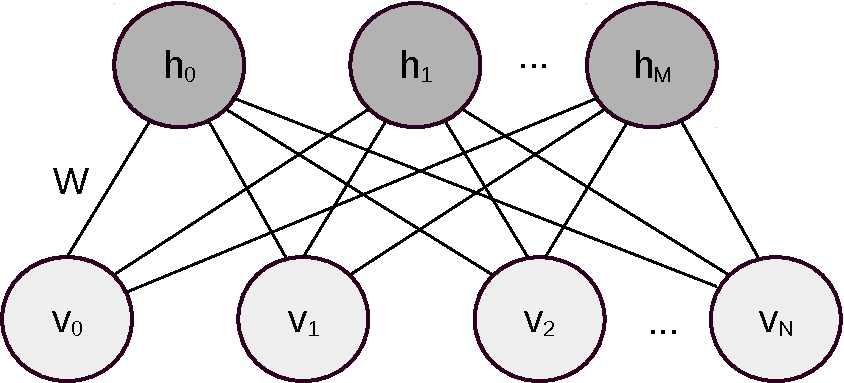
\includegraphics[width=0.6\textwidth]{pics_sdlm/rbm_o.pdf}
	\caption{A typical RBM structure.}
	\label{fig:RBM}
\end{figure}

Despite the various statistical models involved in RBMs and their training method, the actual training algorithm is rather simple thanks to the use of Contrastive Divergence~(CD)~\citep{hinton2002training}.
We can only illustrate some of the statistical models and sampling methods involved in RBM training, a detailed description can be found elsewhere~\citep{fischer2012introduction}. 
Stacked RBMs are also trained by layer-wise greedy algorithms, thus this section will focus on training a single RBM block.

\subsection{Energy-based Model}
In energy-based models, the probability of data point $x$ is defined by a model function $f(x)$, its energy function $E(x)$ and a partition function $Z$ which normalises the model function to possibilities by adding up all possible $f(x)$:
\begin{equation}
%\begin{aligned}
 p(x) = \dfrac{f(x)}{Z}~~, \textrm{~~where~~} f(x) =e^{-E(x)}~~,  \textrm{~~and~~}
 Z = \sum_{x} e^{-E(x)}~~.
%\end{aligned}
\end{equation} 
The energy function~\citep{hopfield1982neural} of an RBM is defined as follows:
\begin{equation}
E(\mathbf{v}, \mathbf{h} \mid \Theta)= -\sum_{i=1}^N a_i v_i - \sum_{j=1}^M b_j h_j - \sum_{i=1}^N \sum_{j=1}^M v_i w_{ij} h_j~~,
\label{equ:energy_complete}
\end{equation}
where the visible layer has $ N $ units, the hidden layer has $ M $, and $ \Theta$ are the model parameters used in RBMs $ \Theta =\{\mathbf{a}, \mathbf{b}, \mathbf{w}\} $ including biases $\mathbf{a}$ and $\mathbf{b}$ on the visible and the hidden layer respectively, and the weights $\mathbf{w}$ between the layers.
As mentioned in Section~\ref{sec:spike}, for simplicity we use neurons without biases in this thesis.
Therefore only the third term of the complete energy function~(Equation~\ref{equ:energy_complete}) is kept:
\begin{equation}
E(\mathbf{v}, \mathbf{h} \mid \Theta)= - \sum_{i=1}^N \sum_{j=1}^M v_i w_{ij} h_j~~,
\label{equ:rbm_energy}
\end{equation}
and the model parameters are reduced to  $ \Theta = \{\mathbf{w}\} $.
Thus the joint probability of the visible vector (input) $\mathbf{v}$ and the output of the hidden units $\mathbf{h}$ is defined as follows: 
\begin{equation}
\begin{aligned}
p(\mathbf{v}, \mathbf{h} \mid \Theta) &=\frac{f(\mathbf{v}, \mathbf{h} \mid \Theta)}{Z(\Theta)}~,  \textrm{~where~} \\
f(\mathbf{v}, \mathbf{h} \mid \Theta) &=e^{-E(\mathbf{v}, \mathbf{h} \mid \Theta)}~,  \textrm{~and~} \\
Z(\Theta) &= \sum_{\mathbf{v}} \sum_{\mathbf{h}} e^{-E(\mathbf{v}, \mathbf{h} \mid \Theta)}~.
\end{aligned}
\label{equ:rbm_prob}
\end{equation}
%However, we are more interested in the marginal probability function: $ p(\mathbf{v} \mid \Theta) $:
%\begin{equation}
%p(\mathbf{v} \mid \Theta) =\frac{\sum_{ \mathbf{h}} e^{-E(\mathbf{v}, \mathbf{h} \mid \Theta)}}{Z(\Theta)}~~,
%\end{equation}	

\subsection{Objective Function}
Given a set of data $ \mathbf{D}=\{\mathbf{v}^1, \mathbf{v}^2, ..., \mathbf{v}^K\} $, the likelihood function of model parameters $\Theta$ defines the probability of the observed outcomes $ \mathbf{D}$ given $\Theta$:
\begin{equation}
L (\Theta \mid \mathbf{D}) = p(\mathbf{D} \mid \Theta ) = \prod_{k=1}^K p(\mathbf{v}^k \mid \Theta ) =  \prod_{k=1}^K\dfrac{f(\mathbf{v}^k \mid \Theta )}{Z( \Theta)}~~.
\label{equ:likelihood}
\end{equation}
Thus the objective is to maximise the likelihood $L (\Theta \mid \mathbf{D})$; that is to say, the model parameters $ \Theta $ that best define the given data $\mathbf{D}$.
Furthermore, in order to simplify the product on the right-hand term in Equation~\ref{equ:likelihood} the objective function can be replaced with the average log-likelihood:
\begin{equation}
\label{equ:like}
\hat{l} (\Theta \mid \mathbf{D}) =\frac{1}{K}\log  L (\Theta \mid \mathbf{D}) 
=\frac{1}{K}\sum_{k=1}^K\log f(\mathbf{v}^k \mid \Theta ) - \log Z( \Theta)~~.
\end{equation}

%Note that, both visible and hidden units have their bias individually, $ \mathbf{a} $ and $ \mathbf{b} $.
%Thus the RBM consists of the data $ \mathbf{D} = \mathbf{V} = (\mathbf{v}_1, \mathbf{v}_2, ..., \mathbf{v}_K ) $, the model parameters $ \Theta = (\mathbf{a}, \mathbf{b}, \mathbf{w}) $ and the hidden units $ \mathbf{h} \sim p(\mathbf{h} \mid \mathbf{v}, \Theta) $.
%
%
%Here we take a Bernoulli-Bernoulli RBM as an example, where each node is a sigmoidal unit.
%The conditional probability function is as follows:
%\begin{equation}
%\begin{aligned}
%& p(h_j = 1 \mid \mathbf{v}) = \sigma(\sum_{i=1}^{M} w_{ij}  v_i + b_j)~,\\
%& p(v_i = 1 \mid \mathbf{h}) = \sigma(\sum_{j=1}^{N} w_{ji}  h_j + a_i)~.
%\end{aligned}
%\end{equation}


%SDG search in parameter space.
%
%Essentially, the integration of the probability model, see Equation~(\ref{equ:z_int}) and~(\ref{equ:z_dis}), is usually algebraically intractable.
%We have to use numerical integration method to evaluate the Equation~(\ref{equ:like}), whose partial derivative is (we are using vectors to generalise the problem):

The derivative of the log-likelihood with respect to a parameter $\theta$ is as follows:
\begin{equation}
\label{equ:part}
\begin{aligned}
\dfrac{\partial \hat{l} (\Theta \mid \mathbf{D})}{\partial \theta} 
& = \frac{1}{K} \dfrac{\partial \sum_{k=1}^K\log f(\mathbf{v}^k \mid \Theta )}{\partial \theta} - \dfrac{\partial \log Z( \Theta)}{\partial \theta}\\
& =  \frac{1}{K}\sum_{k=1}^K \dfrac{\partial \log f(\mathbf{v}^k \mid \Theta)}{\partial \theta} - \sum_x p(\mathbf{x} \mid \Theta) \dfrac{\partial \log f(\mathbf{x} \mid \Theta)}{\partial \theta}\\
& = \left \langle \dfrac{\partial \log f(\mathbf{v} \mid \Theta)}{\partial \theta}\right \rangle_{\mathbf{D}} -\left \langle \dfrac{\partial \log f(\mathbf{v} \mid \Theta)}{\partial \theta}\right \rangle_{\mathbf{C} \sim p(\mathbf{v} \mid \Theta)} ~~,
\end{aligned}
\end{equation}
where $ <\cdot>_{\mathbf{X}} $ denotes the mean expectation of $ \cdot $ given data set $\mathbf{X}$.
The first term of the right-hand side is easy to get with the given data, $\mathbf{d} \in \mathbf{D} $, and the second term can be approximated by generating data samples $\mathbf{C} $ according to $ p(\mathbf{x} \mid \Theta) $.
%These generative samples is called ``fantasy data'' and can be generated using Monte Carlo Markov Chain (MCMC) sampling, see section~\ref{sec:mcmc}.
The detailed derivation process can be found in the Appendix (Equation~\ref{app_equ:part}).
%Although in this example the integration of product of normal distribution is still tractable, it is also helpful to use numerical integration.
%Although $ p(\mathbf{v} \mid \Theta) $ is not a PoE problem, the partial derivation of the average log-likelihood function still applies to Equation~(\ref{equ:part}) and the intractable integration is the same problem here:
Applying the RBM model function (Equation~\ref{equ:rbm_prob}) to the Equation~\ref{equ:part}, we derive the simplified representation of the derivative of the log likelihood:
\begin{equation}
\label{equ:RBM}
\begin{aligned}
\dfrac{\partial \hat{l} (\Theta \mid \mathbf{D})}{\partial \theta} 
& = \left \langle \dfrac{\partial {-E}(\mathbf{v}, \mathbf{h} \mid \Theta)}{\partial \theta} \right \rangle_{\{\mathbf{D}, \mathbf{D}_h \sim p( \mathbf{h} \mid \mathbf{v}, \Theta) \}} 
- \left \langle \dfrac{\partial {-E}(\mathbf{v}, \mathbf{h} \mid \Theta)}{\partial \theta} \right \rangle_{\{\mathbf{C_v}, \mathbf{C_h}\} \sim p( \mathbf{v}, \mathbf{h} \mid  \Theta)},
\end{aligned}
\end{equation}
where the first term of the right-hand side can be gathered from the given data, $ \{\mathbf{D}, \mathbf{D}_h\}$, and the second term will be approximated by sampling $ \{\mathbf{C_v}, \mathbf{C_h}\} $.
Equation~\ref{app_equ:RBM} in the Appendix derives the loss function of RBMs in detail.
Then we plug the RBM energy function (Equation~\ref{equ:rbm_energy}) into the equation above, the loss derivative with respect to the weight is:
\begin{equation}
\label{equ:RBM_2}
%\begin{aligned}
\dfrac{\partial \hat{l} (\Theta \mid \mathbf{D})}{\partial w_{ij}} 
= \left \langle v_i h_j \right \rangle_{\{\mathbf{D}, \mathbf{D}_h \sim p( \mathbf{h} \mid \mathbf{v}, \Theta) \}}
- \left \langle  v_i h_j \right \rangle_{\{\mathbf{C_v}, \mathbf{C_h}\} \sim p( \mathbf{v}, \mathbf{h} \mid  \Theta)}~~. %  \\
%\dfrac{\partial \hat{l} (\Theta \mid \mathbf{D})}{\partial a_{i}} 
%& = \left \langle v_i \right \rangle_{\mathbf{h} \sim p( \mathbf{h} \mid \mathbf{v}, \Theta), \mathbf{V}} 
%- \left \langle  v_i \right \rangle_{\mathbf{v}, \mathbf{h} \sim p( \mathbf{v}, \mathbf{h} \mid  \Theta)},  \\
%\dfrac{\partial \hat{l} (\Theta \mid \mathbf{D})}{\partial b_{j}} 
%& = \left \langle h_j \right \rangle_{\mathbf{h} \sim p( \mathbf{h} \mid \mathbf{v}, \Theta), \mathbf{V}} 
%- \left \langle  h_j \right \rangle_{\mathbf{v}, \mathbf{h} \sim p( \mathbf{v}, \mathbf{h} \mid  \Theta)},  \\
%\end{aligned}
\end{equation}
%\paragraph{CD with 1-step Reconstruction} 
\subsection{Contrastive Divergence}
\label{sec:cd}
Generating data samples for the negative term of Equation~\ref{equ:RBM_2} requires Gibbs sampling on a Markov chain with an infinite number of steps to convergence.
Gibbs sampling approximates the joint probability $p( \mathbf{v}, \mathbf{h} \mid  \Theta)$ with the conditionally probability defined in RBMs:
\begin{equation}
\begin{aligned}
& p(h_j = 1 \mid \mathbf{v}) = \sigma(\sum_{i=1}^{M} w_{ij} v_i)~~,
& p(v_i = 1 \mid \mathbf{h}) = \sigma(\sum_{j=1}^{N} w_{ji} h_j)~~,
\end{aligned}
\label{equ:con_prob}
\end{equation} 
where $\sigma$ represents the Sigmoid activation function for Bernoulli-Bernoulli RBMs.
Figure~\ref{fig:gibbs} illustrates Gibbs sampling on an RBM by $k$ steps where each pair $(\mathbf{v}, \mathbf{h})$ composes a state of the Markov chain, and the joint probability $p( \mathbf{v}, \mathbf{h} \mid  \Theta)$ is approximated by conditional probabilities embedded in the weights (Equation~\ref{equ:con_prob}).

\begin{figure}[hbt]
	\centering
	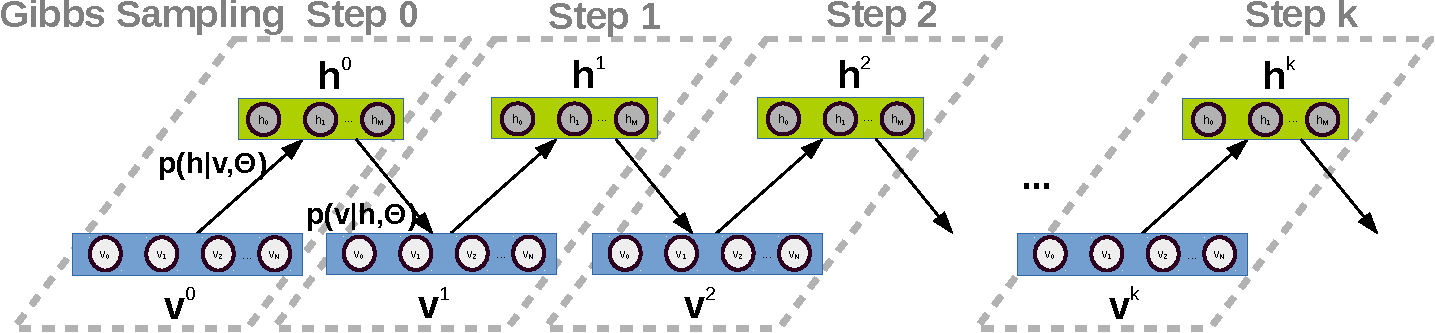
\includegraphics[width=0.98\textwidth]{pics_sdlm/gibbs_sampling.pdf}
	\caption[Gibbs sampling on a RBM.]{Gibbs sampling on a RBM. The method approximates the joint probability $p( \mathbf{v}, \mathbf{h} \mid  \Theta)$ by sampling from conditional probabilities $p( \mathbf{h} \mid  \mathbf{v}, \Theta)$ and $p( \mathbf{v} \mid  \mathbf{h}, \Theta)$. Each sampled data is a pair of $ \mathbf{v}^k$ and $\mathbf{h}^k$.}
	\label{fig:gibbs}
\end{figure}

If $ k \to \infty $, the Markov chain will converge to an equilibrium which represents the distribution of the model-generated data $\{\mathbf{C_v}, \mathbf{C_h}\}$ described by the RBM, and Equation~\ref{equ:RBM} will represent the derivative of the Kullback-Leibler~(KL) divergence with respect to parameter $\theta$.
The KL divergence measures the distance between two probability distributions: the training dataset $\{\mathbf{D}, \mathbf{D_h}\}$ and the generated Gibbs samples, $\{\mathbf{C_v}, \mathbf{C_h}\}$.
However, if we take just a few steps, the KL divergence can be seen as a k-step contrastive convergence ($ \textit{\textrm{CD}}_{k}) $.
Even $ \textit{\textrm{CD}}_1 $ performs surprisingly well in RBM training~\citep{hinton2002training}, which means for every weight update there is only one sample pair $(v^1, h^1)$ generated from Gibbs sampling.
Hence, replacing the mean expectation with 1-step Gibbs sampled data in Equation~\ref{equ:RBM_2}, the RBM training using SGD can be written as follows:
\begin{equation}
\Delta w_{ij} = \eta (v^0_i h^0_j-v^1_i h^1_j)~~,
\label{equ:rbm_train}
\end{equation}
and $v^0_i$ is a given training data, $h^0_j$ is produced with the probability $p( \mathbf{h} \mid \mathbf{v^0_i}, \mathbf{w})$, and the model data pair $(v^1_i, h^1_j)$ is generated by 1-step Gibbs sampling.


%The second term is perfect fit for Gibbs sampling, since we can $ p(\mathbf{v}, \mathbf{h} \mid \Theta) $ as a 2D vector and generating the samples by jumping in a Markov Chain with the transformation probability matrix $ p(\mathbf{v} \mid \mathbf{h}, \Theta) $ and $ p(\mathbf{h} \mid \mathbf{v}, \Theta) $, see Figure~\ref{fig:gibbs} and Section~\ref{sec:Gibbs}.
%So, with the given data $ \mathbf{v}_0 $ and the sampling data $ \mathbf{h}_0 $, we have the initial data point in this Markov Chain,  ($ \mathbf{v}_0, \mathbf{h}_0$).
%The transformation starts from the axis of $ \mathbf{v} $, then we get $ \mathbf{v}_1 \sim p( \mathbf{v} \mid \mathbf{h}_0, \Theta) $.
%It follows the next axis $ \mathbf{h} $, similarly we get $ \mathbf{h}_1 \sim p( \mathbf{h} \mid \mathbf{v}_1, \Theta) $.
%So far we obtain the first sample along the Markov Chain, ($ \mathbf{v}_1, \mathbf{h}_1$) thus to solve the objective function with one iteration.
%The algorithm is described below:   
%\begin{algorithm}[h]
%	\caption{Learning on RBM Parameters with $ CD_1 $}
%	\label{alg:learn}
%	\begin{algorithmic}
%		%			\State Initialisation $\mathbf{x}_0 = [x_0(1),x_0(2),...,x_0(M)]$,  \Comment{Random initialise $\mathbf{x}_0$}
%		\For{$t=1, 2, ..., K$} \Comment{K number of training data $ \mathbf{V} $, 1 data each iteration}
%		%			\For{$k=1, 2, ..., M$}
%		\State $ \mathbf{h}_t \sim p( \mathbf{h} \mid \mathbf{v}_t, \Theta) $
%		\Comment{Generate $ \mathbf{h}_t $ given $ \mathbf{v}_t $ }
%		\State $ \mathbf{v}_{t+1} \sim p( \mathbf{v} \mid \mathbf{h}_{t}, \Theta) $
%		\Comment{Generate $ \mathbf{v}_{t+1} $ on v axis using Gibbs sampling }
%		\State $ \mathbf{h}_{t+1} \sim p( \mathbf{h} \mid \mathbf{v}_{t+1}, \Theta) $
%		\Comment{Generate $ \mathbf{h}_{t+1} $ on h axis using Gibbs sampling }
%		\State $ \dfrac{\partial \hat{l} (\Theta \mid \mathbf{D})}{\partial W_{ij}} = v_{t,i} h_{t,j} - v_{t+1,i} h_{t+1,j}$
%		\State $ \dfrac{\partial \hat{l} (\Theta \mid \mathbf{D})}{\partial a_{i}} = v_{t,i} - v_{t+1,i} $
%		\State $  \dfrac{\partial \hat{l} (\Theta \mid \mathbf{D})}{\partial b_{j}} = h_{t,j} - h_{t+1,j}$
%		\State $ \Delta W_{ij} = \eta ( v_{t,i} h_{t,j} - v_{t+1,i} h_{t+1,j}) $
%		\Comment{Update $ W_{ij} $}
%		\State $ \Delta a_{i} = \eta ( v_{t,i} - v_{t+1,i}) $
%		\Comment{Update $ a_{i} $}
%		\State $ \Delta b_{j} = \eta ( h_{t,j} - h_{t+1,j}) $
%		\Comment{Update $ b_{j} $}
%		%			\EndFor
%		\EndFor
%	\end{algorithmic}
%	\label{alg:rbm}
%\end{algorithm}

\section{Summary}
This chapter briefly introduced the most popular Deep Learning techniques and models for potential use in spiking neural networks.
We illustrated the structure and training procedure for three Deep Learning models: Convolutional Networks, Autoencoders and Restricted Boltzmann Machines, which will be applied in spiking deep networks in the following chapters.
%	\chapter{Noisy Softplus: an Activation Function Enables SNN Training Just Like ANNs}
\label{cha:Conv}
%Paragraph One: LINK
The first step in answering my research question of validating the capability of real-time cognitive application built on neuromorphic platform was to build an object recognition prototype running completely on hardware in an absolute spike-based fashion.
It built up the basis for the later research that neuromorphic hardware has been capable of running large applications standing alone without a general computer and has stepped into the era of improving its cognitive ability.
It is also possible to make a link between this chapter and the whole argument that this work contributes to an effective, straight-forward Spike Neural Network~(SNN) training method which operates exactly as training Artificial Neural Network~(ANN).
In addition the trained model directly fit to SNN without any transformation, and performs almost equivalently to ANNs on cognitive tasks.

%Paragraph Two: FOCUS
%Now focus the reader’s attention on what this chapter is specifically going to do and why it is important. In this chapter I will examine.. I will present… I will report … This is crucial in (aim of thesis/research question) in order to….
The SNN has not achieved the recognition/classification performance of its non-spiking competitor, the ANN, particularly when used in deep neural networks~(DNNs).
Training SNNs by conventional ANN algorithms and mapping well-trained ANNs weights to SNNs are attracting attention in this field for its straight-forward mechanism.
%, especially the SNNs of spiking neurons with biological characteristics.
In this chapter we will propose a new biologically-inspired activation function, Noisy Softplus, which is well-matched to the response firing activity of LIF (Leaky Integrate-and-Fire) neurons.
Thus, any ANN employing Noisy Softplus neurons, even of deep architecture, can be trained simply by the traditional algorithm, for example Back Propagation~(BP), and the trained weights can be directly used in the spiking version of the same network without any conversion.
Furthermore, the training method can be generalised to other activation units, for instance ReLU, to train deep SNNs off-line.
This research is crucial to 1) provide an effective approach for SNN training, and 2) increase the classification accuracy of SNNs with biological characteristics and close the gap between the performance of SNNs and ANNs.

%Paragraph Three: OVERVIEW
%The third paragraph simply outlines the way that you are going to achieve the aim spelled out in the previous paragraph. It’s really just a statement of the contents in the order that the reader will encounter them. It is important to state these not simply as topics, but actually how they build up the internal chapter argument… I will begin by examining the definitions of, then move to seeing how these were applied… I first of all explain my orientation to the research process, positioning myself as a critical scholar.. I then explain the methodology that I used in the research, arguing that ethnography was the most suitable approach to provide answers to the question of… 
%https://patthomson.net/2014/01/16/connecting-chapterschapter-introductions/

%We first of all explore the research question of on-line, event-based deep SNN training in the literature.
%We then describe SRM in mathematical expression, and explain the factors influencing the accuracy of the method and the factors not. 
%Afterwards we argue why the learning algorithm is proper to train spiking Autoencoders (SAEs) and Spiking Restricted Boltzmann Machines (SRBM).
%During the research we encountered the problem introduced by the correlated spikes, therefore we also propose solutions to decorrelate spike trains in Section~\ref{sec:problem}. 
%Finally the detailed comparison of the traditional training and SRM learning on MNIST dataset demonstrates the equivalent learning ability and shows similar even surpassing recognition and reconstruction capability of SAE and SRBM.
In this chapter, we begin by introducing the difficulty of SNN training, and lead to the existing solutions state-of-the-art.
Then we put forward the proposed activation function, Noisy Softplus, and demonstrate how it fits the network dynamics composed of spiking neurons.
Afterwards, a complete SNN training method is explained employing the Noisy Softplus activations and is generalised to other activation functions.
To validate the classification accuracy, a convolutional network (ConvNet) is trained on the MNIST database following this training mechanism and tested directly on an SNN.
The encouraging result demonstrates a close recognition capability of the more biologically-realistic SNNs compared to the conventional ANNs.

\section{Introduction}	
DNNs are the most promising research field in computer vision, even exceeding human-level performance on image classification tasks~\cite{he2015delving}.
To investigate whether brains might work similarly on vision tasks, these powerful DNN models have been converted to SNNs.
In addition, the spiking DNN offers the prospect of neuromorphic systems that combine remarkable performance with energy-efficient training and operation.

Theoretical studies have shown that biologically-plausible learning, e.g. Spike-Timing-Dependent Plasticity (STDP), could approximate a stochastic version of powerful machine learning algorithms
%	~\cite{nessler2013bayesian,neftci2013event,neftci2013event,o2016deep}.
such as 
%	Expectation Maximization~\cite{nessler2013bayesian}, 
Contrastive Divergence~\cite{neftci2013event}, Markov Chain Monte Carlo~\cite{buesing2011neural} and Gradient Descent~\cite{o2016deep}.
It is the stochasticity, in contrast with the continuously differentiable functions used by ANNs, that is intrinsic to the event-based spiking process, making network training difficult.
In practice, ANNs use neuron and synapse models very different from biological neurons, and it remains an unsolved problem to develop SNNs with equivalent performance.

%How to map a well trained ANN to SNN is a hot topic in this field, especially using spiking neurons of biological scale.

Conversely, the offline training of an ANN, which is then mapped to an SNN, has shown near loss-less conversion and state-of-the-art classification accuracy.
These research aim to prove that SNNs are equally capable as their non-spiking rivals of pattern recognition, and at the same time are more biologically realistic and energy-efficient.
Jug et. al.~\cite{Jug_etal_2012} first proposed the use of the Siegert function to replace the sigmoid activation function in training Restricted Boltzmann Machine (RBM).
The Siegert units map incoming currents driven by Poisson spike trains to the response firing rate of a Leaky Integrate-and-Fire (LIF) neuron.
The ratio of the spiking rate to its maximum is equivalent to the output of a sigmoid neuron.
A spiking Deep Belief Network (DBN)~\cite{Stromatias2015scalable} of four layers of RBMs was implemented on neuromorphic hardware, SpiNNaker~\cite{furber2014spinnaker}, to recognise hand written digits in real time.

However, cortical neurons seldom saturate their firing rate.
Thus Rectified Linear Units (ReLU) were proposed to replace sigmoid neurons and surpassed the performance of other popular activation units thanks to their advantage of sparsity~\cite{glorot2011deep} and its robustness towards the vanishing gradient problem. % which will be described in Section~\ref{sec:activation}.
%TODO Chapter2 about relu and vanishing gradient problem.
%	~\cite{dugas2001incorporating}.
%trained with noisy input, the 4-layered spiking autoencoder reached 98.37\% accuracy on MNIST. 
Recent development on ANN-trained SNN models has focused on using ReLU units and converting trained weights to SNNs.
Better performance~\cite{cao2015spiking,diehl2015fast} has been demonstrated in Spiking ConvNets, but this employed simple integrate and fire (IF) neurons without leak.
The training used only ReLUs and zero bias to avoid negative outputs, and applied a deep learning technique, dropout~\cite{srivastava2014dropout}, to increase the classification accuracy.
Normalising the trained weights for use on an SNN employing IF neurons only was relatively straightforward and maintained the classification accuracy.
This work was extended to a Recursive Neural Network (RNN)~\cite{diehl2016conversion} and run on the TrueNorth~\cite{merolla2014million} neuromorphic hardware platform.
Except for the popular, simplified version of ReLU, $max(0,\sum w x)$, the other implementation of $\log(1+e_x)$, Softplus, is more biologically realistic.
Recent work~\cite{hunsberger2015spiking} proposed the Soft LIF response function for training SNNs, which is equivalent to Softplus activation of ANNs.
	
\section{Modelling The Activation Function}
\label{sec:af_model}
We have introduced the existing work of modelling the response firing activity of LIF neurons using Siegert~\cite{Jug_etal_2012} function.
It created the idea of modelling activation functions for spiking neurons whose input is synaptic current generated by spike arrivals and output is the firing rate of a sequence of spike train.
Although the use of Siegert function opened the door for ANN-trained SNNs, there are several drawbacks of this method:
\begin{itemize}
	\item most importantly, the numerical analysis on an LIF response function is too far from the practice, thus it generates large error between the model and the actual response firing rate.
	This issue will be addressed in Section~\ref{subsec:practice}.
	\item the training uses Siegert function to estimate the output firing rate in the forward path, but uses the derivative of sigmoid function during back propagation.
	Due to the difference of Siegert and sigmoid functions, error is introduced. 
	\item high complexity of Siegert function causes much longer training time and more energy.
	\item neurons have to fire at high frequency (higher than half of the maximum firing rate) so as to represent activation of a sigmoid unit, as a result the network activity requires high power dissipation.
	\item better learning performance has been reported using ReLU, so modelling ReLU like activation function of Spiking neurons is needed.  
\end{itemize}

This section will propose the Noisy Softplus function which provides solutions to the drawbacks of Siegert unit.
\subsection{Neural Science Background}
	%As discussed above, most of the top scored networks map the ReLUs in ANN to the equivalent spiking version of IF neurons.
	%This research proposes a new activation function, Noisy Softplus, which is inspired by neuroscience observations of LIF neurons.
	The LIF neuron model follows the following membrane potential dynamics:
	\begin{equation}
	\tau_m \frac{\D V}{\D t}=V_{rest} - V + R_{m} I(t) ~.
	\label{equ:LIF_V}
	\end{equation}
	The membrane potential $V$ changes in response to the input current $I$, starting at the resting membrane potential $V_{rest}$, where the membrane time constant is $\tau_m = R_mC_m$, $R_m$ is the membrane resistance and $C_m$ is the membrane capacitance.
	The central idea in converting spiking neurons to activation units lies in the response function of a neuron model.
	Given a constant current injection $I$, the response function, i.e. firing rate, of the LIF neuron is:
	\begin{equation}
	\lambda_\mathit{out}=
	\left [ t_\mathit{ref}-\tau_m\log \left ( 1-\frac{V_{th}-V_\mathit{rest}}{IR_m}  \right )\right ]^{-1}, \textrm{~when~} IR_m>V_{th}-V_{rest},
	\label{equ:consI}
	\end{equation}
	otherwise the membrane potential cannot reach the threshold $V_{th}$ and the output firing rate is zero. 
	The absolute refractory period $t_\mathit{ref}$ is included, where all input during this period is ignored.
	
	%TODO very important part
	However, in practice, a noisy current generated by the random arrival of spikes, rather than a constant current, flows into the neurons.
	%White noise
	The noisy current is typically treated as a sum of deterministic constant term, $I_{const}$, and a white noise term, $I_{noise}$.
	Thus the value of the current is Gaussian distributed with $m_I$ mean and ${s_I}^2$ variance.
	The white noise is a stochastic process $\xi(t)$ with mean 0 and variance 1, which is delta-correlated, i.e., the process is uncorrelated in time that a value $\xi(t)$ at time $t$ is totally independent of the value at any other time $t'$.
	Therefore, the noisy current can be seen as:
	\begin{equation}
	I(t) = I_{const}(t)+I_{noise}(t) = m_I + s_I\xi(t)~~,
	\label{equ:noisyI}
	\end{equation}
	and accordingly, Equation~\ref{equ:LIF_V} becomes:
	\begin{equation}
	\frac{\D V}{\D t}=\frac{V_{rest} - V}{\tau_m } + \frac{m_I}{C_m} + \frac{s_I\xi(t)}{C_m}~~.
	\label{equ:LIF_V2}
	\end{equation}
	
	We then multiply the both sides of Equation~\ref{equ:LIF_V2} by a short time step $\D t$, the stochastic differential equation of the membrane potential satisfies an Ornstein-Uhlenbeck process:
	\begin{equation}
	\begin{aligned}
	\D V&= \frac{V_{rest} - V}{\tau_m }\D t + \frac{m_I}{C_m} \D t + \frac{s_I}{C_m}  \D W_t \\
	&=\frac{V_{rest} - V}{\tau_m }\D t + \frac{m_I}{C_m} \D t + \frac{s_I \sqrt{\D t}}{C_m} \xi(t)  \\
	&=\frac{V_{rest} - V}{\tau_m }\D t + \mu \D t + \sigma \xi(t) ~~. 
	\end{aligned}
	\end{equation}	
	The last term $\D W_t$ is a Wiener process, that $W_{t +\D t} - W_{t}$ obeys Gaussian distribution with mean 0 and variance $\D t$.
	The instantaneous mean $\mu$ and variance $\sigma^2$ of the change in membrane potential characterise the statistics of $V$ in a short time range, and they can be derived from the statistics of the noisy current:
	\begin{equation}
	\mu =\dfrac{m_I}{C_m}, ~~~~~ \sigma = \dfrac{s_I \sqrt{\D t}}{C_m}~.
	\end{equation}
%	A continuous-time stochastic process W(t) for t>=0 with W(0)=0 and such that the increment W(t)-W(s) is Gaussian with mean 0 and variance t-s for any 0<=s<t, and increments for nonoverlapping time intervals are independent. Brownian motion (i.e., random walk with random step sizes) is the most common example of a Wiener process.
%http://mathworld.wolfram.com/WienerProcess.html
%http://neuronaldynamics.epfl.ch/online/Ch1.S3.html about V tradractory need to write in Chapter 2.	
	The response function~\cite{rauch2003neocortical,la2008response} of the LIF neuron to a noisy current, also known as Siegert formula~\cite{siegert1951first}, is driven by the $\mu$ and $\sigma$:
	\begin{equation}
	\lambda_\mathit{out}=
	\left [ t_\mathit{ref}+\tau_m \int_{\frac{V_\mathit{rest}-\mu \tau_m }{\sigma \sqrt{\tau_m}}}^{\frac{V_{th}-\mu \tau_m }{\sigma \sqrt{\tau_m}}} \sqrt{\pi} \exp(u^{2}) (1+erf(u)) \D u \right ]^{-1} ~,
	\label{equ:siegert}
	\end{equation}
	

	
	\begin{figure}[bt]
		\centering
		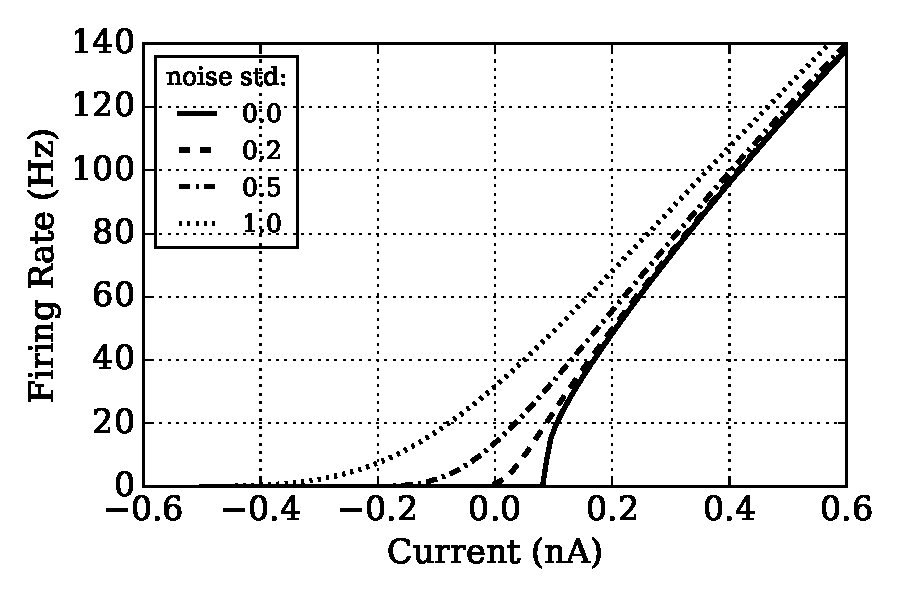
\includegraphics[width=0.7\textwidth]{pics_iconip/1.pdf}
		\caption{Response function of the LIF neuron with noisy input currents with different standard deviations.}
		\label{Fig:physics}
	\end{figure}
	
	Figure~\ref{Fig:physics} shows the response curves (Equation~\ref{equ:siegert}) of a LIF neuron driven by noisy currents with Gaussian noise of $m_I$ mean and $s_I$ standard deviation.
	The parameters of the LIF neuron are all biologically valid (see the listed values in Table~\ref{tbl:pynnConfig}), and the same parameters are used throughout this chapter.
	The solid (zero noise) line in Figure~\ref{Fig:physics} illustrates the response function of such an LIF neuron injected with constant current, which inspired the proposal of ReLUs.
	As noise increases, the level of firing rates also rises, and the Softplus activation function approximates the response firing activity driven by current with Gaussian white noise adding on.
	Softplus units only represent a single level of noise that, for example, the dotted line in Figure~\ref{Fig:physics} is drawn when $s_I=1$.
	
		\begin{table}[bt]
			\centering
			\caption{\label{tbl:pynnConfig}Parameter setting for the current-based LIF neurons using PyNN.}
			\bgroup
			\def\arraystretch{1.4}
			\begin{tabular}{c c c}
				%\hline
				Parameters & Values & Units \\
				\hline
				cm & 0.25 & nF	\\
				%\hline
				tau\_m & 20.0 & ms\\
				%\hline
				tau\_refrac & 1.0 & ms\\
				%					%\hline
				%					tau\_syn\_E & 5.0 & ms\\
				%					%  %\hline
				%					tau\_syn\_I & 5.0 & ms\\
				%  %\hline
				v\_reset & -65.0 & mV\\
				%\hline
				v\_rest & -65.0 & mV\\
				%\hline
				v\_thresh & -50.0 & mV\\
				%\hline
				i\_offset & 0.1 & nA\\
				\hline
				%			Parameters & cm & tau\_m & tau\_refrac & tau\_syn\_E & tau\_syn\_I & v\_rest & v\_thresh & i\_offset \\
				%			Values & 0.25 &  20.0 & 1.0 & 5.0 & 5.0 & -65.0 & -50.0  & 0.1 \\
				%			Units & nF & ms & ms & ms & ms & mV & mV& nA\\
				%			\hline
			\end{tabular}
			\egroup
		\end{table}
	

	


%	\subsection{Activation Function in ANN}
%	\label{sec:activation}
%	Nair and Hinton~\cite{nair2010rectified} stated that ReLU preserve information about relative intensities(intensity equivarance) provided they have zero biases and are noise-free, but binary units do not.
%	This technique has dominated the best recognition performances~\textcolor{red}{ref?} in deep learning.
%	Furthermore, utilising ReLU in SNNs will simplify the network structure significantly because of the zero biases.
%	Thus in this section we firstly demonstrate on how ReLU work and perform in DBN.
%	
%	The input vector in a ReLU based RBM does no longer have to be binary, so it can be a float.
%	Instead of using sigmoid transfer function, the ReLU is always positive and has no upper boundary.
%	There are three different ways to model ReLU~\ref{Fig:relu_tranf}:
%	\begin{figure}[hbt]
%		\centering
%		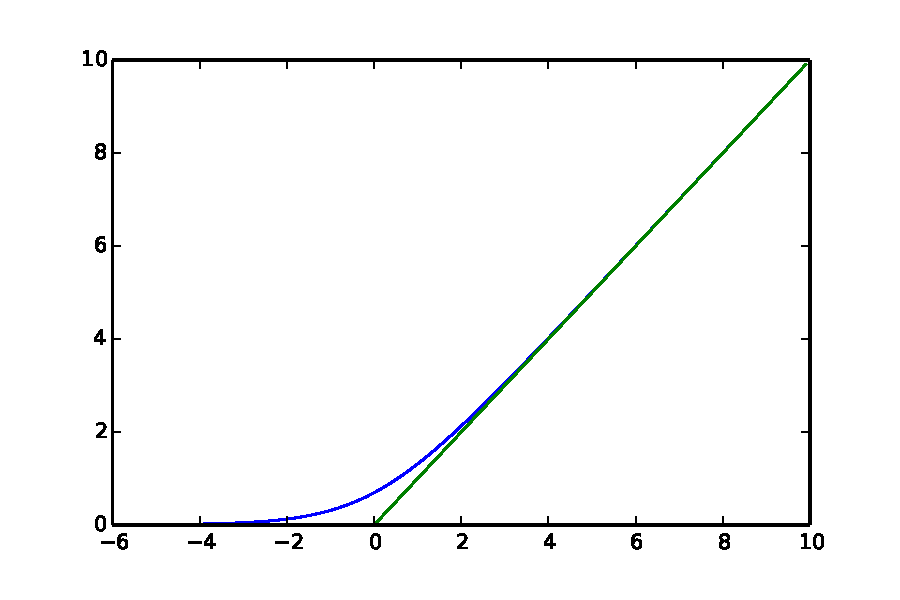
\includegraphics[width=0.7\textwidth]{pics_sdbn/relu.pdf}
%		\caption{The DBN architecture.} 
%		\label{Fig:relu_tranf}
%	\end{figure}
%	\begin{itemize}
%		\item sum of an infinite number of binary units with each having a bias less than the previous one~~\cite{nair2010rectified}.
%		This is one of the reason people believe the recognition performance exceeding since each ReLU represents infinite samples of sigmoid. 
%		\item the approximation of the previous form $\log(1+e_x)$.
%		\item the simplified version which is the most popular in deep learning $max(0,\sum w x)$.
%	\end{itemize}  
	
	
	
	
	\subsection{LIF Neuron Simulation}
	\label{subsec:practice}
	
	
%	\begin{figure}[tbp!]
%		\centering
%		\begin{subfigure}[t]{0.49\textwidth}
%			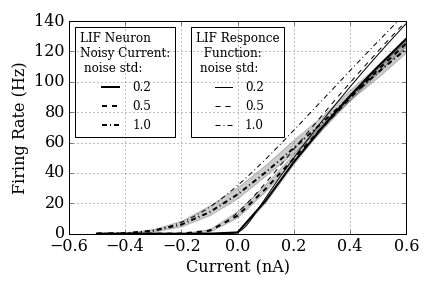
\includegraphics[width=\textwidth]{pics_iconip/2-1.png}
%			\caption{1~ms resolution}
%			\label{Fig:current-1}
%		\end{subfigure}
%		\begin{subfigure}[t]{0.49\textwidth}
%			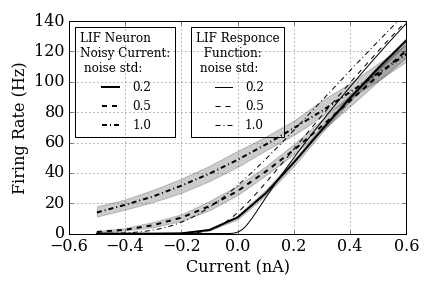
\includegraphics[width=\textwidth]{pics_iconip/2-10.png}
%			\caption{10~ms resolution}
%			\label{Fig:current-10}
%		\end{subfigure}
%		\begin{subfigure}[t]{0.49\textwidth}
%			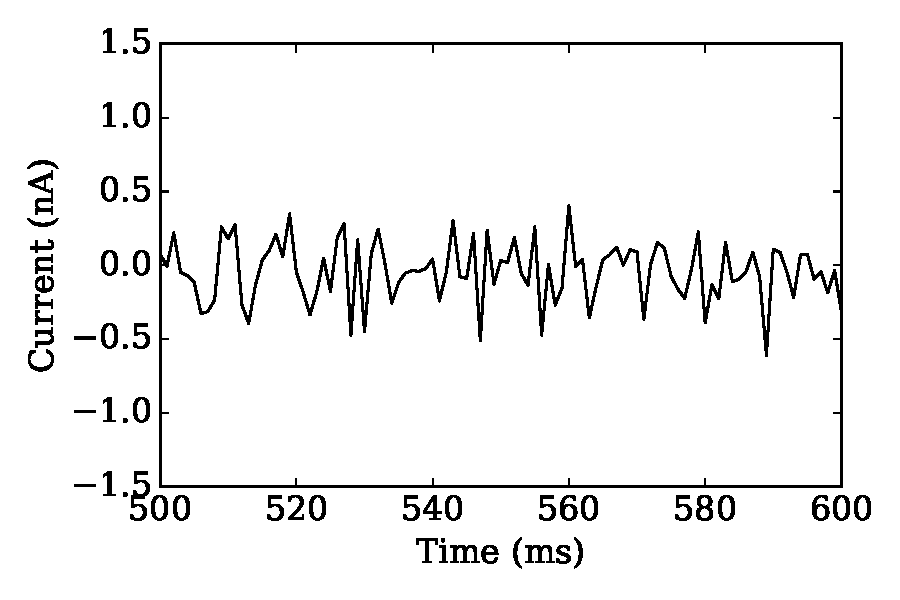
\includegraphics[width=\textwidth]{pics_iconip/curr_dt1.pdf}
%			\caption{1~ms resolution}
%			\label{Fig:signal-1}
%		\end{subfigure}
%		\begin{subfigure}[t]{0.49\textwidth}
%			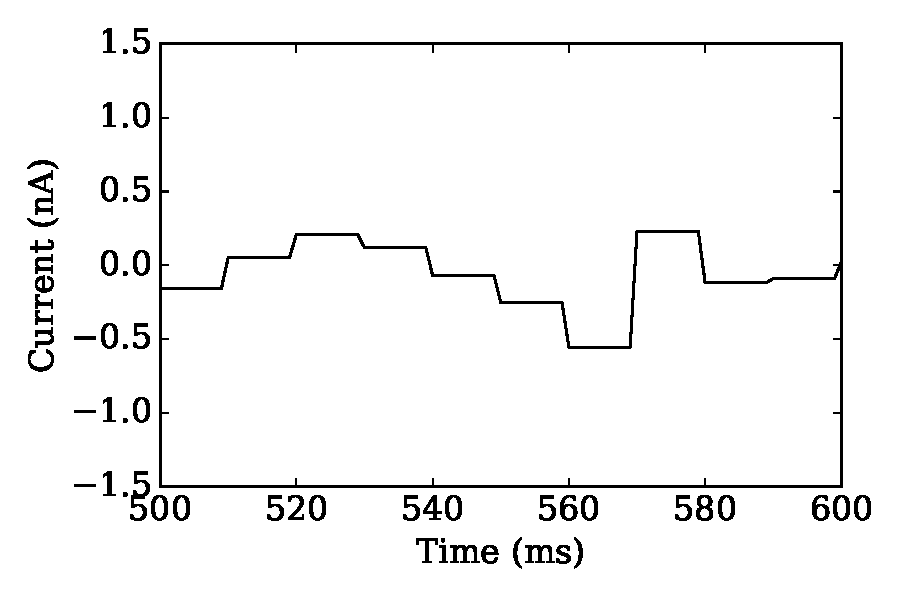
\includegraphics[width=\textwidth]{pics_iconip/curr_dt10.pdf}
%			\caption{10~ms resolution}
%			\label{Fig:signal-10}
%		\end{subfigure}
%		\begin{subfigure}[t]{0.49\textwidth}
%			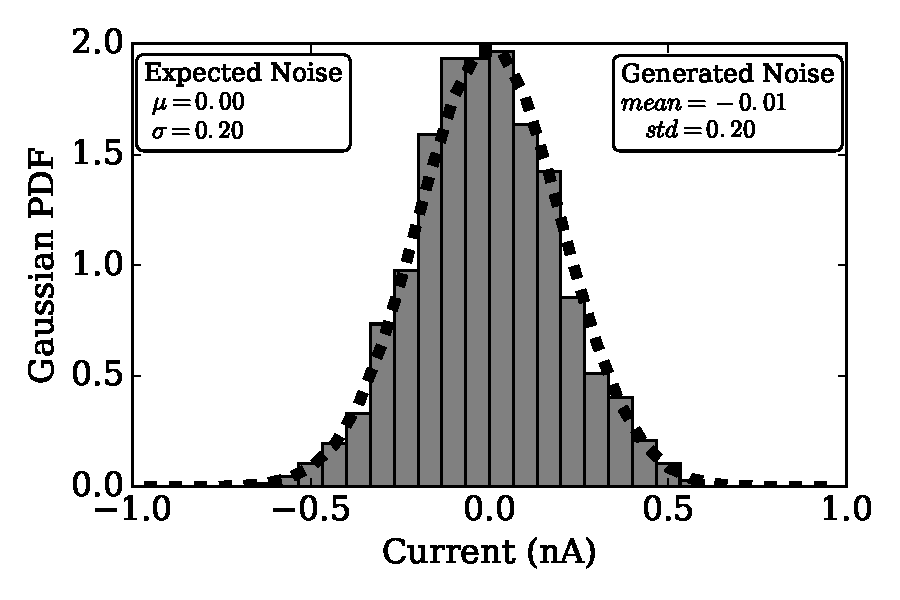
\includegraphics[width=\textwidth]{pics_iconip/distr_dt1.pdf}
%			\caption{1~ms resolution}
%			\label{Fig:gaussian-1}
%		\end{subfigure}
%		\begin{subfigure}[t]{0.49\textwidth}
%			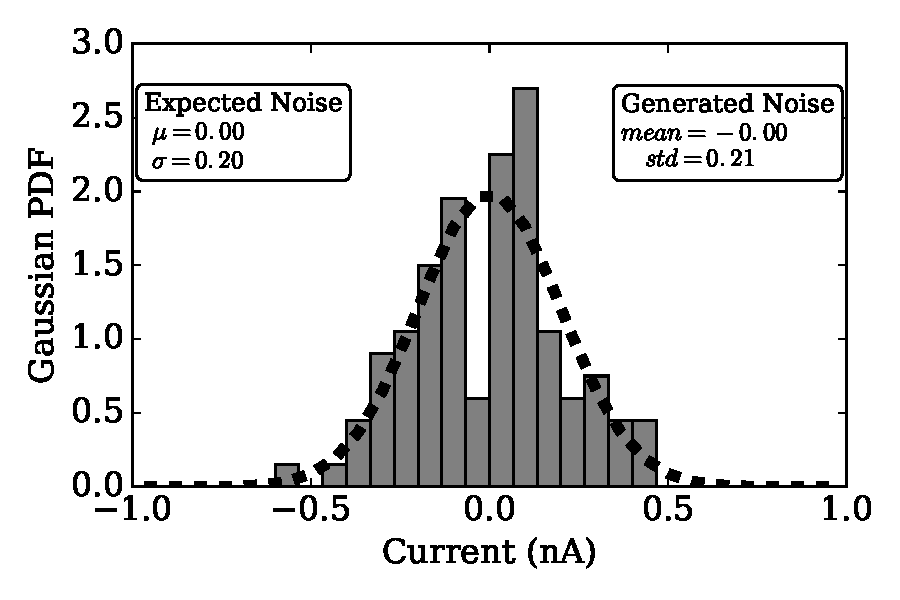
\includegraphics[width=\textwidth]{pics_iconip/distr_dt10.pdf}
%			\caption{10~ms resolution}
%			\label{Fig:gaussian-10}
%		\end{subfigure}
%		\begin{subfigure}[t]{0.49\textwidth}
%			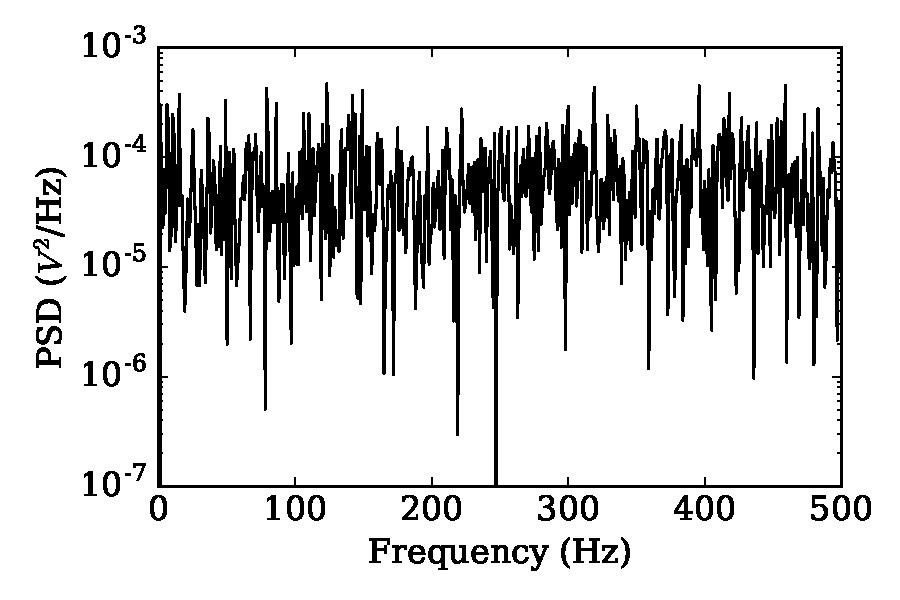
\includegraphics[width=\textwidth]{pics_iconip/psd_dt1.pdf}
%			\caption{1~ms resolution}
%			\label{Fig:spectrum-1}
%		\end{subfigure}
%		\begin{subfigure}[t]{0.49\textwidth}
%			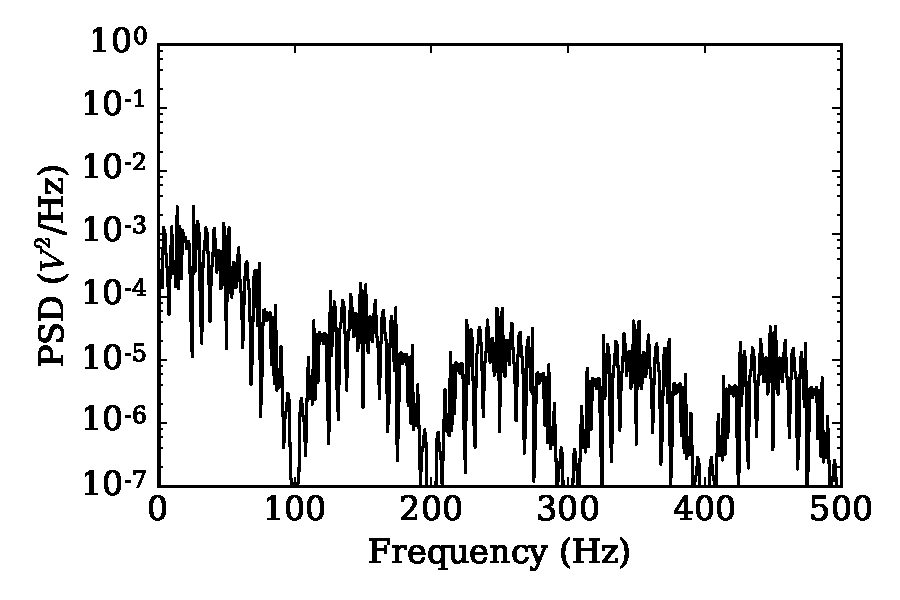
\includegraphics[width=\textwidth]{pics_iconip/psd_dt10.pdf}
%			\caption{10~ms resolution}
%			\label{Fig:spectrum-10}
%		\end{subfigure}
%		\caption{Comparing the recorded firing rates of the LIF neuron simulation driven by noisy currents to the response function shown in Figure~\ref{Fig:physics}.}
%	\end{figure}
\begin{figure}
	\centering
	\begin{subfigure}[c]{0.45\textwidth}\raggedleft
		\myrowlabel{Response Firing Rate}
		\raisebox{-.5\height}{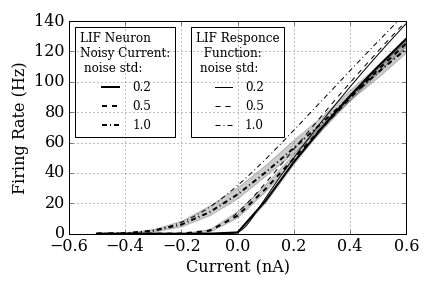
\includegraphics[width=.9\textwidth]
			{pics_iconip/2-1.png}}\\
		\myrowlabel{Current}
		\raisebox{-.5\height}{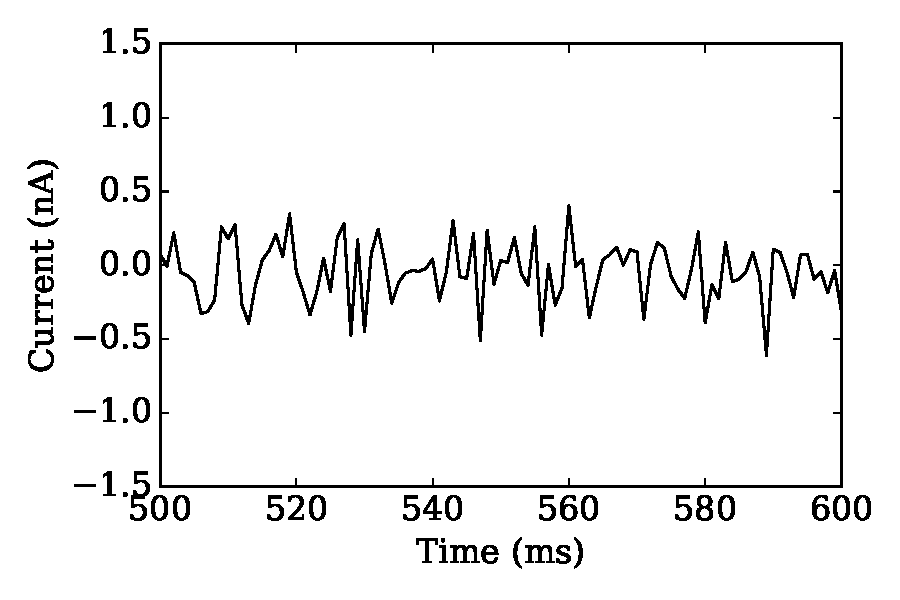
\includegraphics[width=.9\textwidth]
			{pics_iconip/curr_dt1.pdf}}\\
		\myrowlabel{Spectrum Analysis}
		\raisebox{-.5\height}{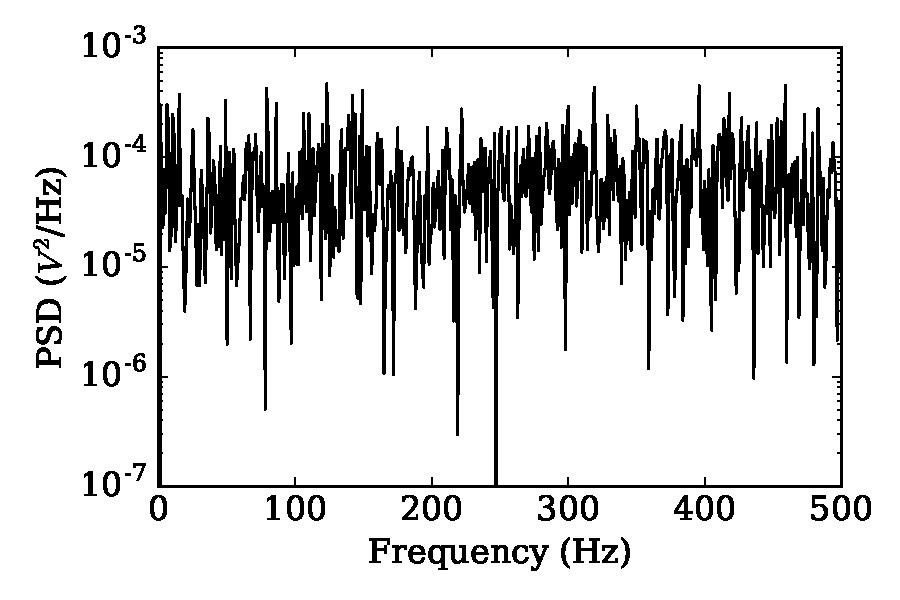
\includegraphics[width=.9\textwidth]
			{pics_iconip/psd_dt1.pdf}}\\
		\myrowlabel{Autocorrelation}
		\raisebox{-.5\height}{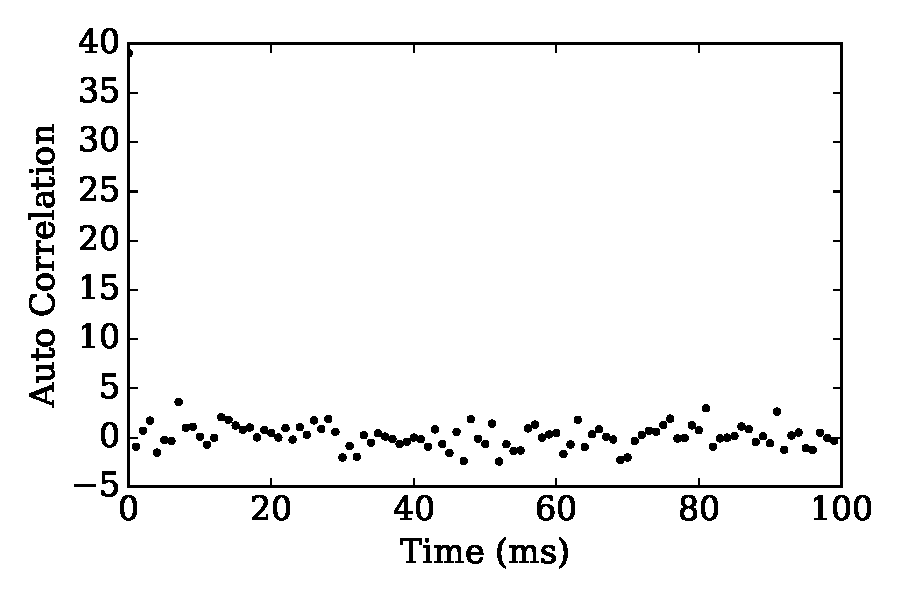
\includegraphics[width=.9\textwidth]
			{pics_iconip/autocorr_dt1.pdf}}\\
		\myrowlabel{Distribution}
		\raisebox{-.5\height}{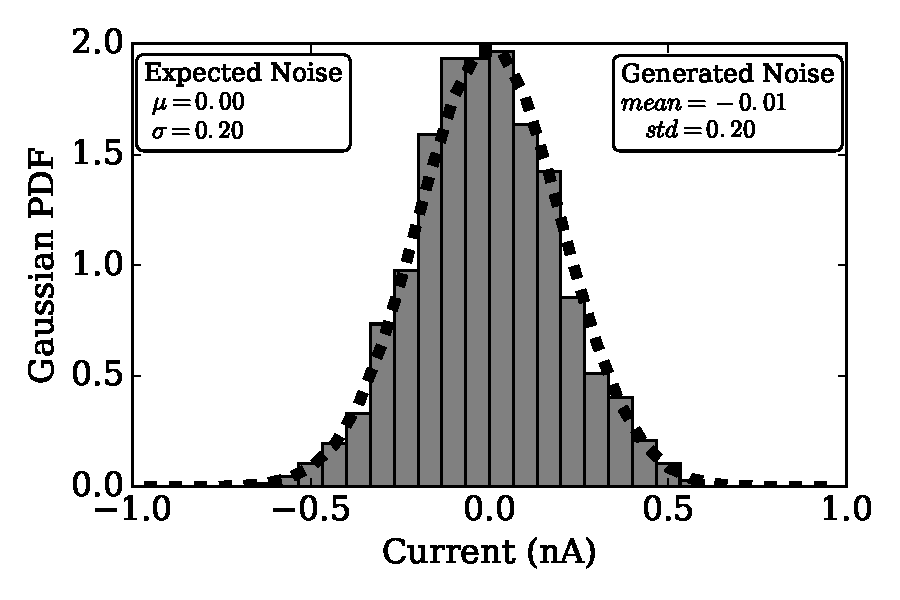
\includegraphics[width=.9\textwidth]
			{pics_iconip/distr_dt1.pdf}}
		\caption{$\tau_{syn}$=1~ms}
	\end{subfigure}%
	\hspace{1em}
	\begin{subfigure}[c]{0.45\textwidth}\raggedleft
		\raisebox{-.5\height}{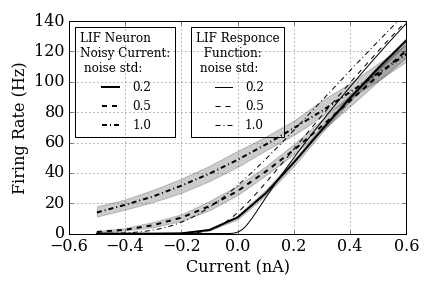
\includegraphics[width=.9\textwidth]
			{pics_iconip/2-10.png}}\\
		\raisebox{-.5\height}{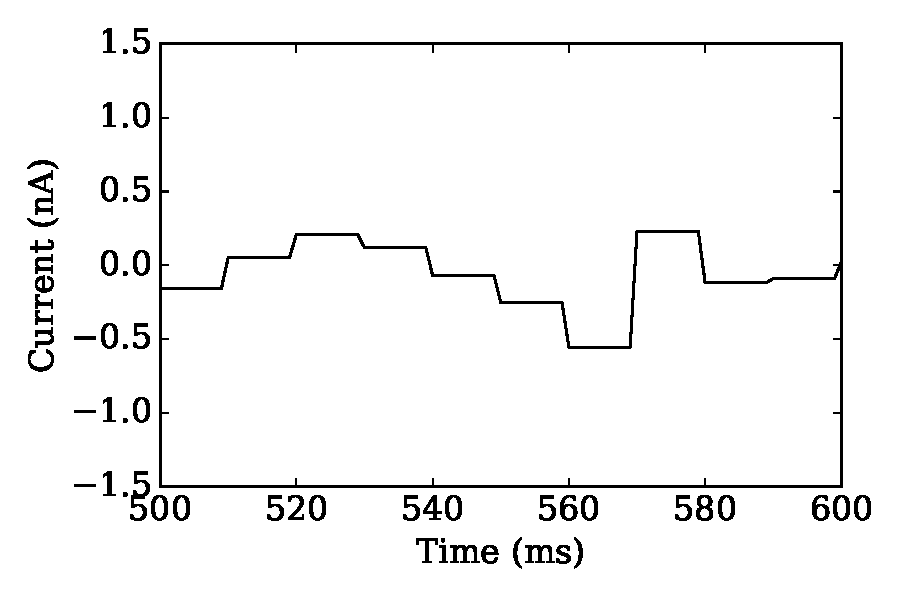
\includegraphics[width=.9\textwidth]
			{pics_iconip/curr_dt10.pdf}}\\
		\raisebox{-.5\height}{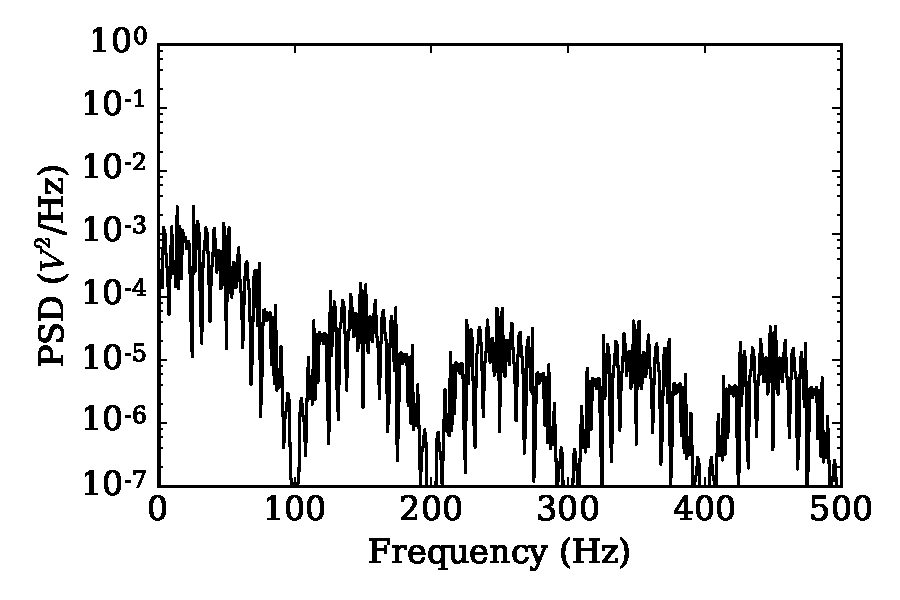
\includegraphics[width=.9\textwidth]
			{pics_iconip/psd_dt10.pdf}}\\
		\raisebox{-.5\height}{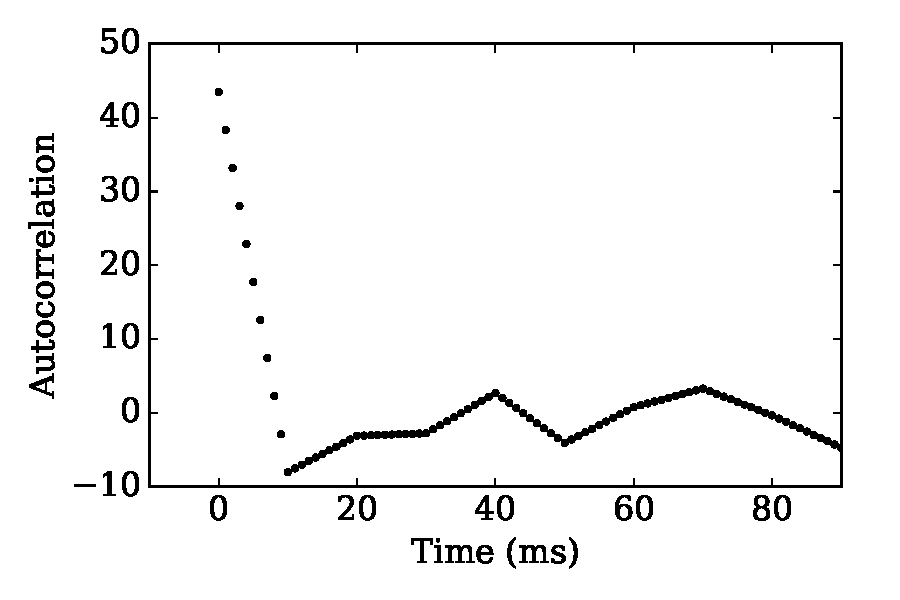
\includegraphics[width=.9\textwidth]
			{pics_iconip/autocorr_dt10.pdf}}
		\raisebox{-.5\height}{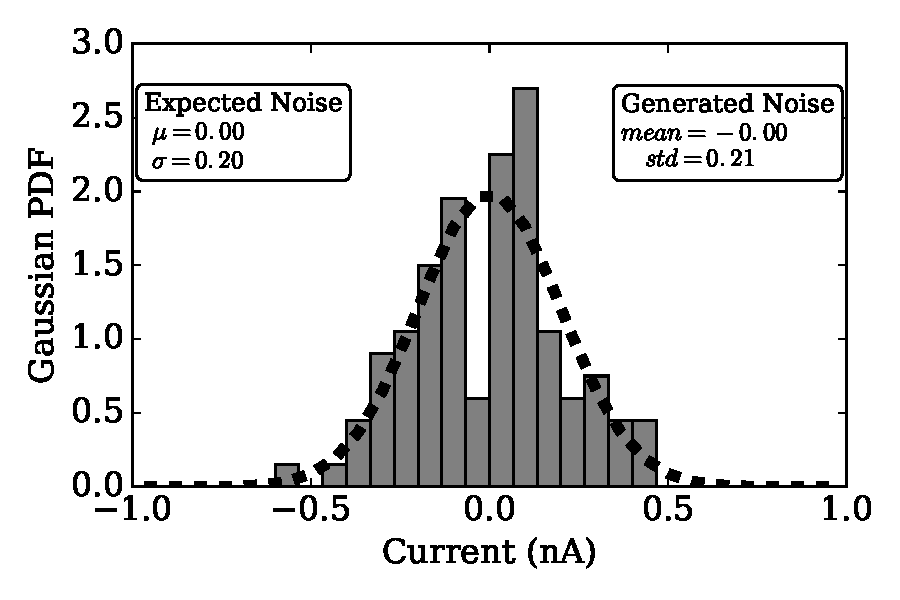
\includegraphics[width=.9\textwidth]
			{pics_iconip/distr_dt10.pdf}}
		\caption{$\tau_{syn}$=10~ms}
	\end{subfigure}%
	\caption{Recorded response firing rate of a LIF neuron driven by noisy current source (bold lines) comparing to the Siegert function (thin lines). The current source is shown in time domain and spectrum domain, so as its autocorrelation, and the distribution. (a) is tested when dt=1~ms, and (b) for dt=10~ms.}
	\label{Fig:lif_curr}
\end{figure}

	To verify the response function in practice, simulation tests were carried out using PyNN~\cite{davison2008pynn} to compare with the analytical results.
	The noisy current was produced by \textit{NoisyCurrentSource} in PyNN which is a constant current of $m_I$ adding up with a Gaussian white noise of zero mean and $s_I^2$ variance.
	The noise was drawn from the Gaussian distribution in a time resolution of $dt$.
	We chose $dt=1$~ms which is the finest resolution for common SNN simulators, and $dt=10$~ms for comparison.
	For a given pair of $m_I$ and $s_I^2$, a noisy current was injected into a current-based LIF neuron for 10~s, and the output firing rate was the average among 10 trials.
	
	The curves of in Figures~\ref{Fig:lif_curr}~[Response Firing Rate] lined up the tests on same noise level.
	The difference compared to the analytical results (thin lines) comes from the time resolution, $dt$, of the \textit{NoisyCurrentSource} see the signals in Figures~\ref{Fig:lif_curr}~[Current].
	The discrete sampling of the noisy current introduces time correlation to the white noise, shown in Figure~\ref{Fig:lif_curr}[Autocorrelation], where the value remains the same within a time step $dt$.
	Although both the current signals followed the same Gauss distribution, see Figures~\ref{Fig:lif_curr}~[Distribution], the current is a white noise when $dt=1$~ms, but a coloured noise when $dt=10$~ms, see Figures~\ref{Fig:lif_curr}~[Spectrum Analysis].
	Thus the Siegert formula, Equation~\ref{equ:siegert}, can only approximate the LIF response of noisy current with white noise.


\begin{figure}
	\centering
	\begin{subfigure}[c]{0.45\textwidth}\raggedleft
		\myrowlabel{Response Firing Rate}
		\raisebox{-.5\height}{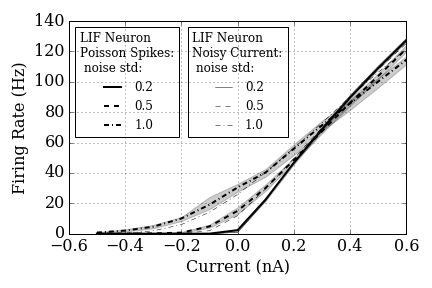
\includegraphics[width=.9\textwidth]
			{pics_iconip/spiked_curve_1.png}}\\
		\myrowlabel{Current}
		\raisebox{-.5\height}{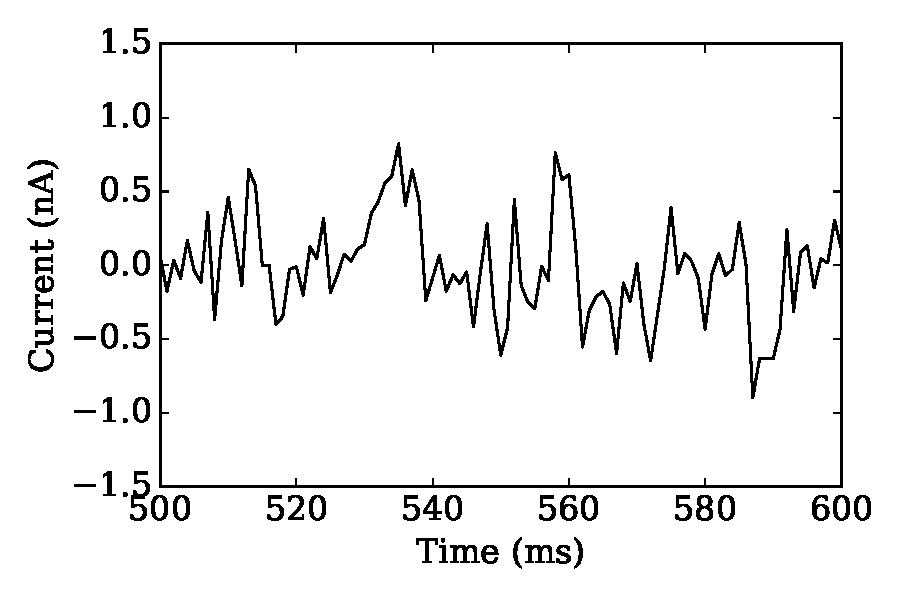
\includegraphics[width=.9\textwidth]
			{pics_iconip/curr_tau1.pdf}}\\
		\myrowlabel{Spectrum Analysis}
		\raisebox{-.5\height}{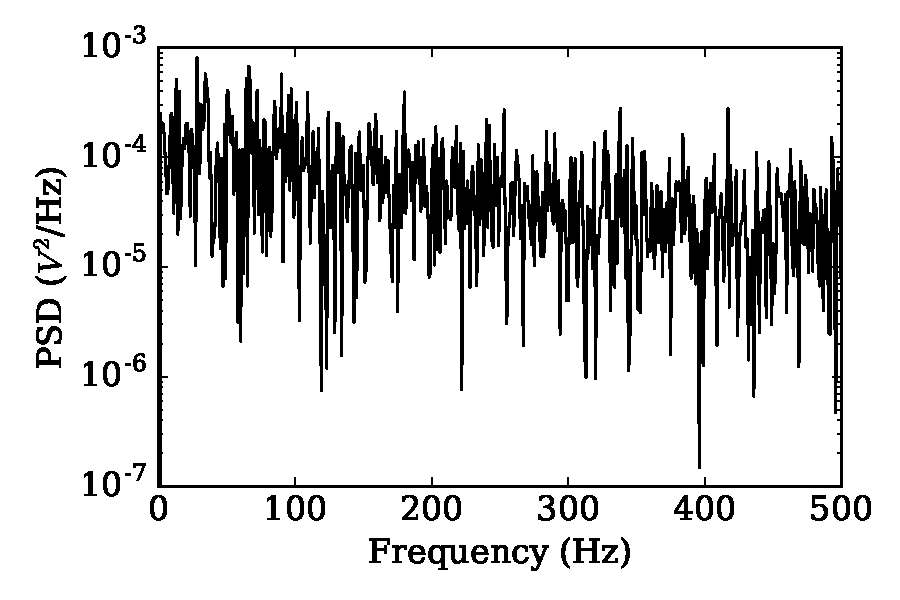
\includegraphics[width=.9\textwidth]
			{pics_iconip/psd_tau1.pdf}}\\
		\myrowlabel{Autocorrelation}
		\raisebox{-.5\height}{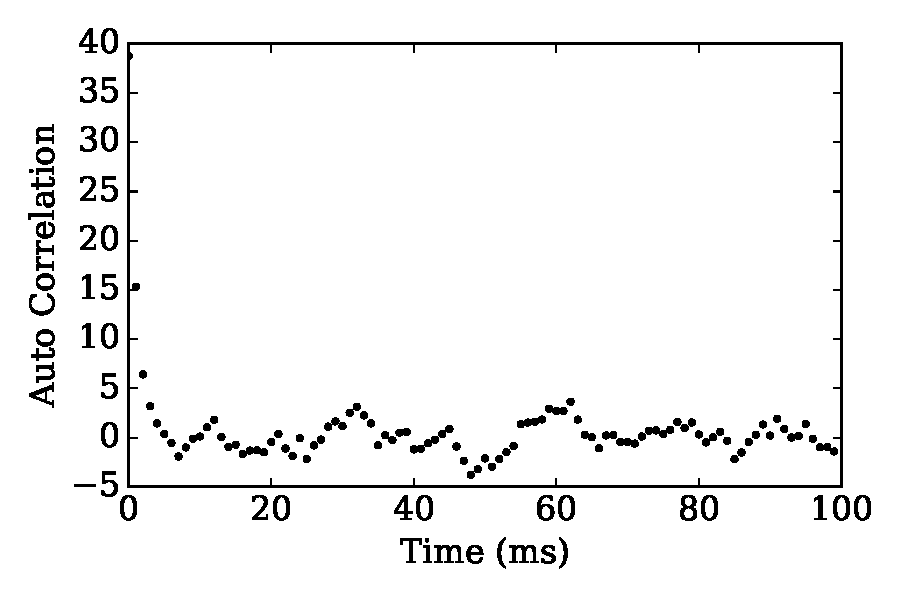
\includegraphics[width=.9\textwidth]
			{pics_iconip/autocorr_tau1.pdf}}\\
		\myrowlabel{Distribution}
		\raisebox{-.5\height}{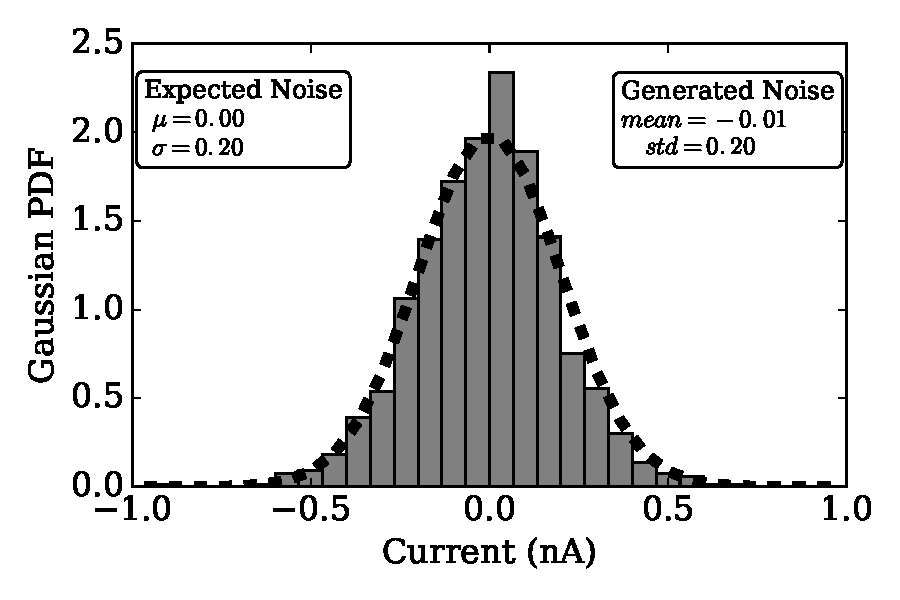
\includegraphics[width=.9\textwidth]
			{pics_iconip/distr_tau1.pdf}}
		\caption{$\tau_{syn}$=1~ms}
	\end{subfigure}%
	\hspace{1em}
	\begin{subfigure}[c]{0.45\textwidth}\raggedleft
		\raisebox{-.5\height}{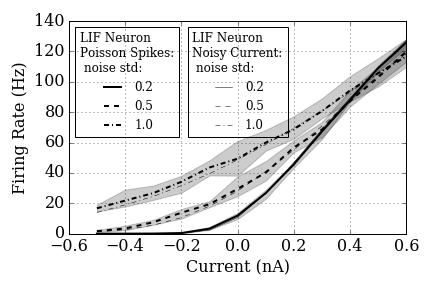
\includegraphics[width=.9\textwidth]
			{pics_iconip/spiked_curve_10.png}}\\
		\raisebox{-.5\height}{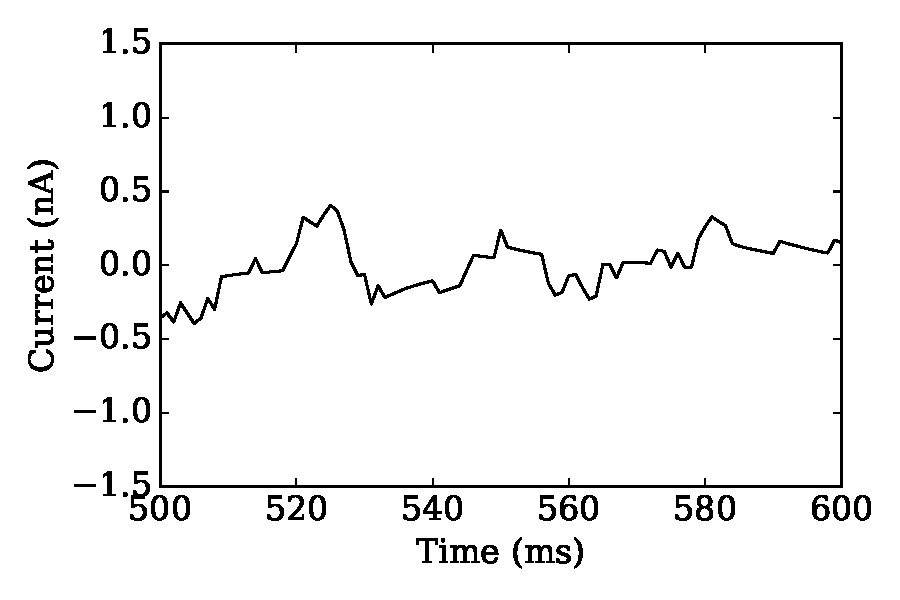
\includegraphics[width=.9\textwidth]
			{pics_iconip/curr_tau10.pdf}}\\
		\raisebox{-.5\height}{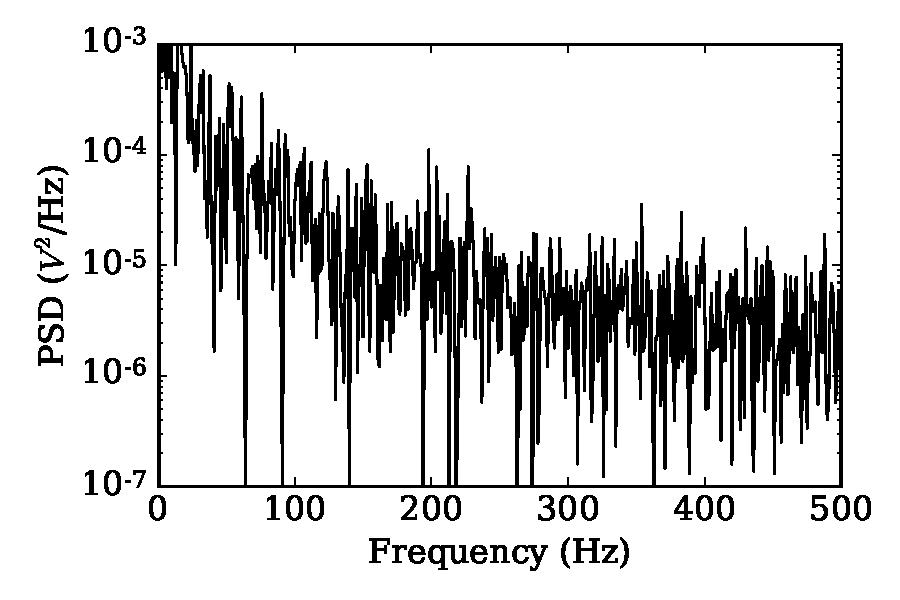
\includegraphics[width=.9\textwidth]
			{pics_iconip/psd_tau10.pdf}}\\
		\raisebox{-.5\height}{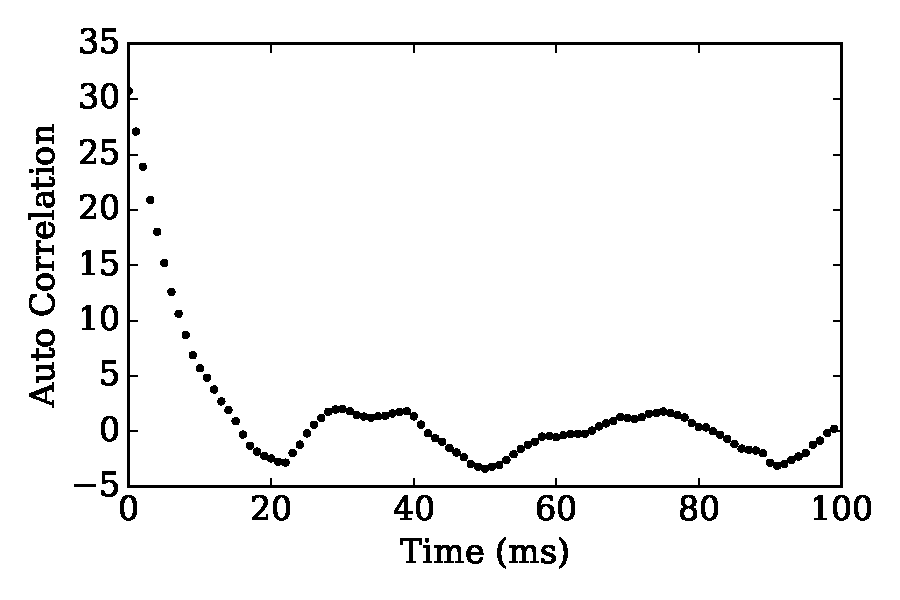
\includegraphics[width=.9\textwidth]
			{pics_iconip/autocorr_tau10.pdf}}
		\raisebox{-.5\height}{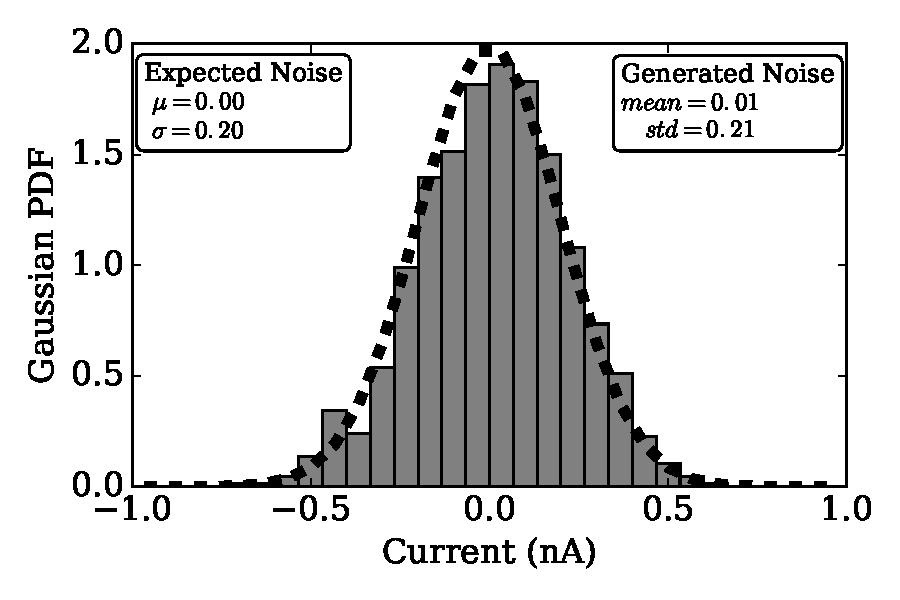
\includegraphics[width=.9\textwidth]
			{pics_iconip/distr_tau10.pdf}}
		\caption{$\tau_{syn}$=10~ms}
	\end{subfigure}%
	\caption{Recorded response firing rate of a LIF neuron driven by synaptic current (bold lines) comparing to the noisy current source (thin lines). The synaptic current is shown in time domain and spectrum domain, so as its autocorrelation, and the distribution. (a) is tested when $\tau_{syn}$=1~ms, and (b) for $\tau_{syn}$=10~ms.}
	\label{Fig:lif_pois}
\end{figure}
	
%\begin{figure}[btp!]
%	\centering
%	\begin{subfigure}[t]{0.49\textwidth}
%		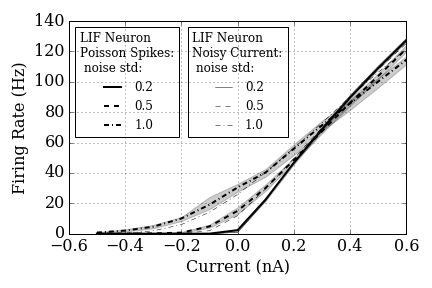
\includegraphics[width=\textwidth]{pics_iconip/spiked_curve_1.png}
%		\caption{$\tau_{syn}$=1~ms}
%	\end{subfigure}
%	\begin{subfigure}[t]{0.49\textwidth}
%		\includegraphics[width=\textwidth]{pics_iconip/spiked_curve_10.png}
%		\caption{$\tau_{syn}$=10~ms}
%	\end{subfigure}
%	\begin{subfigure}[t]{0.49\textwidth}
%		\includegraphics[width=\textwidth]{pics_iconip/curr_tau1.pdf}
%		\caption{$\tau_{syn}$=1~ms}
%	\end{subfigure}
%	\begin{subfigure}[t]{0.49\textwidth}
%		\includegraphics[width=\textwidth]{pics_iconip/curr_tau10.pdf}
%		\caption{$\tau_{syn}$=10~ms}
%	\end{subfigure}
%	\begin{subfigure}[t]{0.49\textwidth}
%		\includegraphics[width=\textwidth]{pics_iconip/distr_tau1.pdf}
%		\caption{$\tau_{syn}$=1~ms}
%	\end{subfigure}
%	\begin{subfigure}[t]{0.49\textwidth}
%		\includegraphics[width=\textwidth]{pics_iconip/distr_tau10.pdf}
%		\caption{$\tau_{syn}$=10~ms}
%	\end{subfigure}
%	\begin{subfigure}[t]{0.49\textwidth}
%		\includegraphics[width=\textwidth]{pics_iconip/psd_tau1.pdf}
%		\caption{$\tau_{syn}$=1~ms}
%	\end{subfigure}
%	\begin{subfigure}[t]{0.49\textwidth}
%		\includegraphics[width=\textwidth]{pics_iconip/psd_tau10.pdf}
%		\caption{$\tau_{syn}$=10~ms}
%	\end{subfigure}
%
%\end{figure}

	A more realistic simulation of a noisy current is generated by 100 Poisson spike trains, 
	%assuming that large amount of small amplitude PSPs are required to reach the threshold and $\tau_syn$ limits to 0.
	where the mean and variance of the current are given by:
	\begin{equation}
	m_I = \tau_{syn}\sum_i w_i\lambda_{i}~, ~s_I^2=\frac{1}{2}\tau_{syn}\sum_i w_i^2\lambda_{i}~,
	\label{equ:distr}
	\end{equation}
	where $\tau_{syn}$ is the synaptic time constant, and each Poisson spike train connects to the neuron with a strength of $w_i$ and a firing rate of $\lambda_i$.
	Two populations of Poisson spike sources, for excitatory and inhibitory synapses respectively, were connected to a single LIF neuron to mimic the noisy currents.
	The firing rates of the Poisson spike generators were determined by the given $m_I$ and $s_I$.
	Figures~\ref{Fig:lif_pois}~[Response Firing Rate] illustrate the recorded firing rates responding to the spike trains compared to the mean firing rate driven by \textit{NoisyCurrentSource}.
	Note that the estimation of LIF response activity requires noisy current with white noise, however
%	The use of noisy currents assumes that the post-synaptic potential (PSP) is a delta function, e.g. $\tau_{syn}$ tends to the limits of 0.
	in practice the release of neurotransmitter takes time ($\tau_{syn} >> 0$) and the synaptic current decays exponentially $I_{syn} = I_0 e^{\frac{-t}{\tau_{syn}}}$.
	Figures~\ref{Fig:lif_pois}~[Current] show two examples of synaptic current of 0~nA mean and 0.2 standard deviation driven by 100 neurons firing at the same rate and with the same synaptic strength (half excitatory, half inhibitory), but of different synaptic time constant.
	Therefore, the current at any time t during decaying period is dependant to the value at previous time step, which makes the synaptic current a coloured noise, see Figures~\ref{Fig:lif_pois}~[Spectrum Analysis].
%	and the noise added to the mean current is not white noise, but pink noise.
	We observe in Figure~\ref{Fig:lif_pois}~[Response Firing Rate](a) that the response firing rate to synaptic current is higher than the \textit{NoisyCurrentSource} for all the 10 trials.
	It is caused by a) the coarse resolution (1~ms) of the spikes, thus the standard deviation of the current is larger than 0.2, shown in Figure~\ref{Fig:lif_pois}~[Distribution](a);
	and b) the $\tau_{syn}$, even short as 1~ms, adds coloured noise instead of white noise to the current.
	While Figure~\ref{Fig:lif_pois}~[Distribution](b) shows a similar firing rate of both the synaptic driven current and the \textit{NoisyCurrentSource}, since both of the current signals have similar distribution and time correlation.
	Nevertheless, the analytical response function, Siegert formula, cannot approximate the practical simulations.
	
%	Thus the experiments show that a longer $\tau_{syn}$ increases the level of noise and widens the variance of the output firing rate.
	

		
	\subsection{Noisy Softplus}
	Therefore, due to the limited time resolution of common SNN simulators and the time taken for neurotransmitter release, $\tau_{syn}$, mismatches exist between the analytical response function, Siegert formula, and the practical neural activities.
	Consequently, a unified activation function is required to model the practical responses of a LIF neuron.
	Inspired by the set of response functions triggered by different levels of noise, we propose the Noisy Softplus activation function:
	\begin{equation}
	y = f_{ns}(x, \sigma) = k \sigma \log [1 + \exp(\frac{x}{k \sigma})],
	\label{equ:nsp}
	\end{equation}
	where $x$ refers to the mean current, $y$ indicates the strength of the output firing rate, $\sigma$ plays an important role to define the noise level, and $k$, which is determined by the neuron parameters, controls the shape of the curves.
	Note that the novel activation function we propose contains two parameters, the current and its noise; both are naturally obtained in spiking neurons.
	% With doubled information, more powerful training methods and network models are expected. 
	Figure~\ref{fig:nsp} shows the activation function in curve sets corresponding to different discrete noise level, and in a 3D plot.
	\begin{figure}[thb!]
		\centering
		\begin{subfigure}[t]{0.7\textwidth}
			\includegraphics[width=\textwidth]{pics_iconip/4.pdf}
			\caption{Noisy Softplus}
		\end{subfigure}\\
		\begin{subfigure}[t]{0.8\textwidth}
			\includegraphics[width=\textwidth]{pics_iconip/5.pdf}
			\caption{Noisy Softplus in 3D}
		\end{subfigure}
		\caption{
			Noisy Softplus fits to the response function of the LIF neuron.
			Noisy Softplus in (a) curve sets and (b) 3D.}
		\label{fig:nsp}
	\end{figure}	
	
	The derivative is the logistic function scaled by $k\sigma$:
	\begin{equation}
	\frac{\partial f_{ns}(x,\sigma)}{\partial x} = \frac{1}{1+exp(-\frac{x}{k\sigma})}~~,
	\label{equ:logist}
	\end{equation}	
	which could be easily applied to back propagation in any network training.
	
	The activation function can be scaled up by a factor, $S$, to represent the firing rate $\lambda$ of a LIF neuron driven by a noisy current $x$.
	\begin{equation}
	\begin{aligned}
	\lambda_{out} &\simeq f_{ns}(x, \sigma) \times S\\
	&=k \sigma \log [1 + \exp(\frac{x}{k \sigma})] \times S
	\end{aligned}
	\label{equ:fit}
	\end{equation}	
	
	The Noisy Softplus fits well to the practical response firing rate of the LIF neuron with suitable calibration of $k$ and $S$, see Figure~\ref{Fig:nsptau1}.
	The parameter pair of $(k, S)$ is curve-fitted with the triple data points of $(\lambda, x, \sigma)$.
	The fitted parameter was set to $(k, S)=(0.19,208.76)$ for the practical response firing rate driven by synaptic noisy current with $\tau_{syn}=1$~ms and was set to $(k, S)=(0.35,201.06)$ when $\tau_{syn}=10$~ms.
	The calibration currently is conducted by linear least squares regression, however numerical analysis is considered for future work to express the factors with biological parameters of a LIF neuron.
	
	\begin{figure}
		\centering
		\begin{subfigure}[t]{0.49\textwidth}
			\includegraphics[width=\textwidth]{pics_iconip/4-1.png}
			\caption{$\tau_{syn}$=1~ms}
		\end{subfigure}
		\begin{subfigure}[t]{0.49\textwidth}
			\includegraphics[width=\textwidth]{pics_iconip/4-10.png}
			\caption{$\tau_{syn}$=10~ms}
		\end{subfigure}
		\caption{Noisy Softplus fits to the response firing rates of LIF neurons.}
		\label{Fig:nsptau1}
	\end{figure}		
	
	
\section{ANN-Trained SNNs}	
	We have discussed modelling response firing activity of a LIF neuron with a unified activation function, Noisy Softplus.
	However the demonstration of mapping the physical activity to numerical ANN calculations is still required, thus to train the layered-up deep network.
	
	\subsection{Equivalent Input and Output}
	
	\begin{figure}[bt]
		\centering
		\includegraphics[width=0.7\textwidth]{pics_iconip/neuron.pdf}
		\caption{Artificial neuron model in ANNs. }
		\label{Fig:neuron}
	\end{figure}
	Neurons in ANNs take inputs from their previous layer, and feed the weighted sum of their input, $net_j = \sum_i w_{ij}x_i$, to the activation function.
	The transformed signal then forms the output of an artificial neuron, $y_j=f(net_j)$, see Figure~\ref{Fig:neuron}.
	
	Meanwhile, Noisy Softplus is able to predict the firing rate of a spiking neural driven by some noisy current, nevertheless an extra step is still needed to map the firing rate to numerical values in ANNs.
	According to Equation~\ref{equ:distr}, the mean of the current feeding into a spiking neuron is equivalent to $net$ of artificial neurons, where
	\begin{equation}
	\begin{aligned}
		& {m_I}_j = \sum_i w_{ij}(\lambda_{i}\tau_{syn})~, \textrm{  then}\\
		& net_j= \sum_i w_{ij} x_i~~, \textrm{~~and~~}
		x_i = \lambda_{i}\tau_{syn}~.
	\end{aligned}
	\label{equ:mi_input}
	\end{equation}
	The noise level of Noisy Softplus, $\sigma^2$, is the variance of the current, which also can be seen as a weighted sum of the same input $x$ but with different weights:
	\begin{equation}
	\begin{aligned}
		& {s_I^2}_j=\sum_i(\frac{1}{2} w_{ij}^2) (\lambda_{i}\tau_{syn})~, \textrm{  then}\\
		& \sigma^2_j= \sum_i (\frac{1}{2} w_{ij}^2) x_i~~.
	\end{aligned}
	\label{equ:si_input}
	\end{equation}
	
	\begin{figure}[bt!]
		\centering
		\includegraphics[width=0.98\textwidth]{pics_iconip/neuron_o.pdf}
		\caption{Artificial spiking neuron takes scaled firing rates as input, then transforms weighted sum in some activation unit to its output which can be scaled-up to the firing rate of an output spike train.}
		\label{Fig:sneuron}
	\end{figure}
	
	Noisy Softplus transforms the noisy current with parameters of $(net_j, \sigma_j)$ to the equivalent ANN output $y_j$ , where it can be scaled up by the scaling factor $S$ to the firing rate of SNNs.
	Note that the calculation of noise level is not necessary for activation functions other than Noisy Softplus, for example, it can be set to a constant for Softplus or 0 for ReLU.
	We name the neuron model `artificial spiking neurons' which takes firing rates of spike trains as input and output. 
	The entire artificial spiking neuron model is then generalised to any ReLU/Softplus-like activation functions, See Figure~\ref{Fig:sneuron}.
	

	
	
	\subsection{Layered-up Network}
	
%	Figure~\ref{Fig:sneuron} shows an complete transformation process of a spiking neuron, which mimics the biological neurons taking and generating spike trains.
	If we move the left end process of $\times \tau_{syn}$ to the right hand side, Figure~\ref{Fig:sneuron} forms the same model structure as artificial neurons shown in Figure~\ref{Fig:neuron}: neurons takes $x$ as input and outputs $y$, See Figure~\ref{Fig:tneuron}.
	The process within an artificial neuron is divided to weighted summation and activation, which also applied to the spiking neuron model by combining the scaling factor $S$ and the synaptic time constant $\tau_{syn}$ to activation functions.
	Thus the combined activation function for modelling SNNs should be:
	\begin{equation}
	y = f(x) \times S \times \tau_{syn}~~.
	\label{equ:full_act}
	\end{equation}
	\begin{figure}[tbh!]
		\centering
		\includegraphics[width=0.8\textwidth]{pics_iconip/neuron_t.pdf}
		\caption{Transforming artificial spiking neurons to artificial neurons for SNN modelling. The combined activation links the firing activity of a spiking neuron to the numerical value of ANNs.}
		\label{Fig:tneuron}
	\end{figure}
	
	
	
	The derivative function used when back propagates is:
	\begin{equation}
	\frac{\partial y}{\partial x} = f'(x) \times S \times \tau_{syn}~~.
	\end{equation}
	

	
	Thus, using this method of ANN-trained SNNs, the activation functions are of lower complexity than Siegert formula, and their corresponding derivative functions can be directly used for back propagation.
	Furthermore, the method enables ReLU-like activation functions for SNN training, thus to improve the recognition accuracy while keeping a relative lower firing rate compared to sigmoid neurons. 
	Most significantly, the ANN-trained weights are ready for use in SNNs without any transformation, and the output firing rate of a spiking neuron can be estimated in the ANN simulation.
	
	
	\subsection{Fine Tuning}
	The labels of data are always converted to binary values for ANN training.
	This enlarges the disparities between the correct recognition label and the rest to train the network for better classification capability.
	Consequently, we train the network as stated above (with any activation function) and then fine tuning it with Noisy Softplus in order to take account of both accuracy and practical network activities of SNNs.
	However, we add a small number, for example 0.01, to all the binary values of the data labels, and use Noisy Softplus as activation function for fine tuning. 
	By doing so, it helps the training to loosen the strict objective function to predict exact with binary values.
	Instead, it allows a small offset to the objective.
	An alternative method is to use Softmax function at the last layer, which aims to map real vectors to the range of $(0,1)$ that add up to 1. 
	However, without a limit on the input of Softmax, it will be easy to reach or even exceed the highest firing rate of a spiking neuron.
	
	There are two aspects in the fine tuning which makes the ANN more close to SNNs:
	Firstly, using Noisy Softplus activation functions in a whole trained network operates every single neuron running in a similar noise level as in SNNs, thus the weights trained by other activation functions will be tuned to fit more closely to SNNs.
	Secondly, the output firing rate of any LIF neuron is greater than zero as long as noise exists in their synaptic input.
	Thus adding up a small offset on the labels directs the model to approximate to practical SNNs. 
	The result of fine tuning on a Convnet will be demonstrated in the Section~\ref{subsec:result_compare}.
	
	
\section{Results}
\label{sec:iconipResult}
	A convolutional network model was trained on MNIST,
	%	~\cite{lecun1998gradient}
	a popular database in neuromorphic vision, using the ANN-trained SNN method stated above.
	The architecture contains $28\times28$ input units, followed by two convolutional layers 6c5-2s-12c5-2s, and the 10 output neurons fully connected to last pooling layer represent the classified digit.
	
	The training employed Noisy Softplus units only that all the convolution, average sampling, and the fully-connected neurons use Noisy Softplus function with no bias.
	The parameters of the activation function were calibrated as, $(k=0.30, S=201)$,  for LIF neurons~(see~Tablel~\ref{tbl:pynnConfig}) of $\tau_{syn}=5$~ms.
	The input images were scaled by 100~Hz to present the firing rates of input spikes.
	The weights were updated using a decaying learning rate, 50 images per batch and 20 epochs.
	The ANN-trained weights were then directly applied in the corresponding convolutional SNN without any conversion for recognition tasks.
	
	
	\subsection{Neural Activity}
	Firstly, to validate how well the Noisy Softplus activation fits to the response firing rate of LIF neurons in a real application, we simulated the model on Nest using the Poisson MNIST dataset~\cite{liu2016bench} and the neurons of a convolutional map were observed.
	
		\begin{figure}[tbh!]
		\centering
		\begin{subfigure}[t]{0.8\textwidth}
			\includegraphics[width=\textwidth]{pics_iconip/6-1.png}
			\caption{10 input digits presented in Poisson spike trains in raster plot}
			\label{Fig:61}
		\end{subfigure}\\
		\begin{subfigure}[t]{0.3\textwidth}
			\includegraphics[width=\textwidth]{pics_iconip/6-2.pdf}
			\caption{Pixel firing rates}
			\label{Fig:62}
		\end{subfigure}
		\begin{subfigure}[t]{0.3\textwidth}
			\includegraphics[width=\textwidth]{pics_iconip/6-3.pdf}
			\caption{5x5 kernel}
			\label{Fig:63}
		\end{subfigure}
		\begin{subfigure}[t]{0.3\textwidth}
			\includegraphics[width=\textwidth]{pics_iconip/6-4.pdf}
			\caption{Output firing rates}
			\label{Fig:64}
		\end{subfigure}
		\caption{Images presented in spike trains convolve with a weight kernel. (a) The $28\times28$ Poisson spike trains in raster plot, representing 10 digits in MNIST. (b) The firing rate of all the 784 neurons of the fourth image, digit `0', is plotted as a 2D image.
		(c) One out of six of the trained kernels ($5\times5$ size) in the first convolutional layer.
		(d) The spike trains plotted as firing rate of the neurons in the convolved 2D map.}
		\label{fig:cnn}
	\end{figure}

	Figure~\ref{fig:cnn} shows a small test of ten MNIST digits presented in Poisson spike trains for 1~s each.
	A trained $5\times5$ kernel (Figure~\ref{fig:cnn}(c)) were convolved with these input digits, and the fourth digit `0' (Figure~\ref{fig:cnn}(b)) and its convolved output of the feature map was shown in Figure~\ref{fig:cnn}(d) as firing rate.
	The output firing rate was recorded during a real-time SNN simulation on NEST, and compared to the modelled activations of Equation~\ref{equ:full_act} in ANNs.
	
	The input $x$ of the network was calculated as Equation~\ref{equ:mi_input}: $x_i=\lambda_i\tau_{syn}$, and so as the weighted sum of the synaptic current (see Equation~\ref{equ:mi_input}), $net_j$ and its variance (see Equation~\ref{equ:si_input}), $\sigma^2_j$.
	With three combined activation functions as Equation~\ref{equ:full_act}:
	\begin{equation}
	\begin{aligned}
	&\textrm{(1) Noisy Softplus:~~}  y_j=k \sigma_j \log [1 + \exp(\frac{net_j}{k \sigma_j})] \times S \times \tau_{syn}~~,  \\
	&\textrm{(2) ReLU:~~ } y_j=max(0, net_j) \times S \times \tau_{syn}~~, \\
	&\textrm{(3) Softplus:~~ } y_j=k \sigma \log [1 + \exp(\frac{net_j}{k \sigma})] \times S \times \tau_{syn}~~, ~~~\sigma=0.45,  
 	\end{aligned}
	\end{equation}	
	we compare the output to the recorded SNN simulations.
	ReLU assumes a non-noise current, and Softplus takes a static noise level thus $\sigma_j$ is not used for either of them, meanwhile Noisy Softplus adapts to noise automatically with $\sigma_j$.
	The experiment took the sequence of 10 digits shown in Figure~\ref{fig:cnn}(a) to the same kernel and the estimated spike counts using Noisy Softplus fit to the real recorded firing rate much more accurately than ReLU and Softplus,  see~\ref{fig:af_compare}.
%	Figure~\ref{fig:af_stast} illustrated the statistics of error between the estimation and the recorded firing rate, $err = y_j - \lambda_j$ which formed normal distributions where Noisy Softplus hold the weakest mean (low in abstract) and lowest standard deviation.
	The Euclidean distance, $\sqrt{\sum_{j}(y_j/\tau_{syn} - \lambda_j)}$, between the spike counts and the predicted firing rates by Noisy Softplus, ReLU and Softplus was 184.57, 361.64 and 1102.76 respectively.
	We manually selected a static noise level of 0.45 for Softplus, whose estimated firing rates located roughly on the top slope of the real response activity.
	Which resulted in longer Euclidean distance than using ReLU, since most of the input noisy currents were of relatively low noise level in this experiment.
	In another word, the firing rate driven by lower noise level is closer to ReLU curve than Softplus.
	
			
	\begin{figure}[tbh!]
		\centering
		\begin{subfigure}[t]{0.8\textwidth}
			\includegraphics[width=\textwidth]{pics_iconip/6-5.png}
		\end{subfigure}
		\caption{
			Noisy Softplus fits to the neural response firing rate in an SNN simulation.
			The recorded firing rate of the same kernel convolved with 10 images shown in Figure~\ref{fig:cnn} in SNN simulation, comparing to the prediction of activations of Noisy Softplus, Softplus and ReLU.}
		\label{fig:af_compare}
	\end{figure}
	
	Figure~\ref{Fig:out} demonstrates the output firing rates of the 10 recognition neurons when tested with the digit sequence.
	The SNN successfully classified the digits where the correct label neuron fired the most.
	We trained the network with binary labels on the output layer, thus the expected firing rate of correct classification was $1/\tau_{syn}=200$~Hz according to Equation~\ref{Fig:tneuron}.
	The firing rates of the recognition test fell to the valid range around 0 to 200~Hz.
	This shows another advantage of the proposed ANN-trained method that we can constrain the expected firing rate of the top layer, thus to prevent SNN from exploding its maximum firing rate, for example 1000~Hz when time resolution of SNN simulation set to 1~ms.
	
		\begin{figure}[tbp!]
			\centering
			\includegraphics[width=0.7\textwidth]{pics_iconip/7.pdf}
			\caption{Output firing rates for recognising 10 hand written digits.}
			\label{Fig:out}
		\end{figure}
	
	\subsection{Recognition Performance}
	\label{subsec:result_compare}
	Secondly we focus on the recognition performance of the proposed ANN-trained SNN method.
	Before we reach there, it is significant to see the learning capability of the proposed activation function, Noisy Softplus.
	We compared the training using ReLU, Softplus, and Noisy Softplus by their loss during training averaged over 3 trials, see Figure\ref{Fig:loss_ns}.
	ReLU learned the fastest and reached the lowest loss, thanks to its steepest derivative and none-noise assumption.
	To the contrary, Softplus accumulated spontaneous firing rates layer by layer and its derivative may experience gradients vanish during back propagation, which result in a more difficult training.
	Noisy Softplus performed in between in terms of loss and learning speed.
	However, the loss stabilised the fastest, which means a possible shorter training time.
	\begin{figure}[tbp!]
		\centering
		\includegraphics[width=0.7\textwidth]{pics_iconip/8.png}
		\caption{Comparisons of Loss during training using Noisy Softplus, ReLU and Softplus activation functions. Bold lines show the average of three training trials, and the grey colour fills between the minimum and the maximum of the trials.  }
		\label{Fig:loss_ns}
	\end{figure}
%	The trained networks were scaled to SNNs and compared on recognition rates, 93.34\%, 96.43\% and 97.03\% with a conversion loss of 4.76\%, 0.91\% and 0.74\%.
	
	The recognition test took the whole testing dataset of MNIST which contains $10,000$ images.
	At first, all the trained models were tested on the same artificial neurons as used for training in ANNs, and these experiments were called `DNN' test since the network had a deep structure (5 layers).
	Afterwards, the trained weights were then directly applied to SNN without any transformation, and these `SNN' experiments tested their recognition performance on NEST simulator.
	The LIF neurons had the same parameters as in training.
	The input images were converted to Poisson spike trains and presented for 1~s each.
	The output neuron which fired the most predicted the classification of an input image.
	Moreover, 'Fine tuning' test took the trained model for fine tuning, and the tuned weights were tested on the same SNN environment.
	The tuning only ran for one epoch, 5\% cost of the ANN training, using Noisy Softplus neurons with labels shifted for $+0.01$.
	
	The classification error for all the tests are listed in Table~\ref{tbl:ns_result} and the averaged classification accuracy is shown in Figure~\ref{Fig:result_bar}.
	From DNN to SNN, the classification accuracy declines by 0.80\%, 0.79\% and 3.12\% in average for Noisy softplus, ReLU and Softplus
	The accuracy loss was caused by the mismatch between the activations and the practical response firing rates, see example in Figure~\ref{fig:af_compare}, and the strict binary labels for Noisy Softplus and Softplus activations.
	Fortunately, the problem is alleviated by fine tuning which increased the classification accuracy by 0.38\%, 0.19\% and 2.06\%, and resulted in the total loss of 0.43\%, 0.61\%, and 1.06\% respectively.
	The improvement of ReLU is not as much as the others, because there is no problem of strict labels during training.
%	Thus fine tuning mainly corrects the mismatch between ReLU and the firing rates in SNNs, and constraints the output firing rates of the network.
	While Softplus benefits the most from fine tuning, since not only the huge mismatch of response firing rate is much corrected, but also the loosed labels helps the network to fit SNNs. 
	
	\begin{figure}[hbt!]
		\centering
		\includegraphics[width=0.7\textwidth]{pics_iconip/9-2.pdf}
		\caption{Classification accuracy compared among trained weights of Noisy Softplus, ReLU, Softplus on DNN, SNN and fine-tuned SNN.}
		\label{Fig:result_bar}
	\end{figure}
	
	\begin{table}[tbh] 
		\caption{Comparisons of classification accuracy (in \%) of ANN-trained convolutional neural models on original DNN, NEST simulated SNN, and SNN with fine-tuned (FT) model.}
		\begin{center}
			\bgroup
			\def\arraystretch{1.5}
			\begin{tabular} {r |c  c c |c c c |c c c}
				%First line
				\hline
				Trial No.
				&\multicolumn{3}{c|}{1} 
				&\multicolumn{3}{c|}{2}
				&\multicolumn{3}{c}{3}\\
				\hline
				Model
				& DNN & SNN &FT
				& DNN & SNN &FT
				& DNN & SNN &FT\\
				\hline
				\textbf{Noisy Sofplus}
				& 1.91 & 2.76 &2.45
				& 1.79 & 2.56 &2.19
				& 1.76 & 2.55 &2.10\\
%				& 98.09 & 97.24 &97.55
%				& 98.21 & 97.44 &97.81
%				& 98.24 & 97.45 &97.90\\
%				\hline
				\textbf{ReLU}
				& 1.36 & 2.03 &1.88
				& 1.46 & 2.28 &2.00
				& 1.36 & 2.25 &2.12\\
%				& 98.64 & 97.97 &98.12
%				& 98.54 & 97.72 &98.00
%				& 98.64 & 97.75 &97.88\\
%				\hline
				\textbf{Sofplus}
				& 2.30 & 5.66 &3.91
				& 2.75 & 5.22 &3.55
				& 2.42 & 6.62 &3.87\\
%				& 97.70 & 94.34 &96.09
%				& 97.25 & 94.78 &96.45
%				& 97.58 & 93.38 &96.13\\
				\hline
			\end{tabular}
			\egroup
			\label{tbl:ns_result}
		\end{center}
	\end{table}
	
	
	
	
	The best classification accuracy achieved by SNNs was 98.12\%, 0.53\% drop from ANN test, which was trained with ReLU and fine-tuned by Noisy Softplus.
	The most efficient training in terms of both classification accuracy and algorithm complexity, takes ReLU for ANN training and Noisy Softplus for fine tuning.
	Softplus does not exhibit better classification capability and more importantly the manual selected static noise level hugely influences the mismatch between the predicted firing rates and the real data.
	Although Noisy Softplus shows the least classification drop from ANNs to SNNs, the training performance is still worse than ReLU.
	Improved back propagation or other learning algorithms using noise level will be listed in the future work. 
	
		
	\begin{figure}[htb!]
		\centering
		\begin{subfigure}[t]{0.49\textwidth}
			\includegraphics[width=\textwidth]{pics_iconip/8-2.png}
		    \caption{Before fine tuning}
		\end{subfigure}
		\begin{subfigure}[t]{0.49\textwidth}
			\includegraphics[width=\textwidth]{pics_iconip/8-3.png}
		    \caption{After fine tuning.}
		\end{subfigure}

		\caption{The classification accuracy of 3 trials (averaged in bold lines, grey lines show the range between minimum to maximum) over short response times, with (a) trained weights before fine tuning, and (b) after fine tuning.}
		\label{fig:ca_time}	
	\end{figure}
	
	As it is a major concern in neuromorphic vision, the recognition performance over short response times is also estimated in Figure~\ref{fig:ca_time}.
	After fine tuning Softplus significantly reduced the mismatch, since the randomness among the three trials shrinks to similar range to other experiments.
	More obviously fine tuning improved its classification accuracy and the response latency.
	Notice that all of the networks trained by three different activation functions showed a very similar stabilisation curve against time, which means they all reached a close accuracy to their best taking 300~ms of test. 
	
	
	\subsection{Power Consumption}
	Noisy Softplus can be easily used for energy cost estimation for SNNs.
	For a single neuron, the energy consumption of the synaptic events it triggers is:
	\begin{equation}
	\begin{aligned}
	E_{j} &= \lambda_j N_j T E_{syn}\\
	&= \dfrac{y_j N_j T E_{syn}}{\tau_{syn}}~~,
	\end{aligned}
	\end{equation}
	where $\lambda_j$ is the output firing rate, $N_j$ is the number of post-synaptic neurons it connects to, $T$ is the testing time, and $E_{syn}$ is the energy cost for a synaptic event of some specific neuromorphic hardware, for example, about 8~nJ on SpiNNaker~\cite{stromatias2013power}.
	Thus to estimate the whole network, we can sum up all the synaptic events of all the neurons:
	\begin{equation}
	\sum_j E_{j} =  \dfrac{T E_{syn}}{\tau_{syn}} \sum_{j}y_j N_j.
	\end{equation}
	Thus, it may cost SpiNNaker 0.064~W, thus 192~J running for $3,000$~s on synaptic events to classify $10,000$ images (300~ms each) with the best accuracy of 98.02\%.
	
\section{Summery}
%\section{Discussions}
	Most significantly, we proposed the Noisy Softplus activation function which accurately models response firing rate of LIF neurons and solved the drawbacks of Siegert units.
%	 listed in Section~\ref{sec:af_model}: 
%	\begin{itemize}
%		\item Noisy Softplus takes account of time correlation of the noisy synaptic current, e.g. $\tau_{syn}$, which fits more to the actual response firing rate.
%		
%		\item Noisy Softplus can be applied easily to any training method, for example BP, thanks to its derivative function defined in Equation~\ref{equ:logist}.
%		
%		\item the calculation on Noisy Softplus is no more than Softplus function, except for doubled computation on weighted sum of its input ($net$ and $\sigma$ in Equations~\ref{equ:mi_input} and~\ref{equ:si_input}), which is much more simplified than Siergert function.
%		
%		\item as one of the ReLU-liked activation function, the output firing rate seldom exceed the working range of a LIF neuron, for example the firing rates were around 0-200~Hz in the ConvNet model.
%		
%		\item the learning performance of Noisy Softplus is between Softplus and ReLU, which is supposed to outperform most of the other popular activation functions: for instance sigmoid.
%	\end{itemize}

	Moreover, we put forward the complete SNN modelling method by using artificial neurons of combined activation.
	This method can be generalised to activation units other than Noisy Softplus.
	The training of an SNN model is exactly the same as ANN training, and the trained weights can be directly used in SNN without any transformation.
	This method is more simpler and even more straight forward than the other ANN offline training methods which requires an extra step of converting ANN-trained weights to SNN's.
	
	In terms of classification/recognition accuracy, the performance of ANN-trained SNNs is nearly equivalent as ANNs, and the performance loss can  be partially solved by fine tuning.
%	The best classification accuracy of 98.12\% using LIF neurons in PyNN simulation outperforms most of the SNN models of LIF neurons which will be listed in Chapter~6, and is closely to the result using IF neurons~\cite{diehl2015fast}. 
	

	%A conclusion should be a short summary of the most pithy points in the chapter. It’s the thing that you’re going to leave the reader with. Given that they’ve just spent time reading the whole chapter, they don’t want to read it all again. What do you most want the reader to remember about this chapter? What is the key to the argument you’ve made, the most significant thing(s) that they have to keep in their mind as they go forward? In a thesis, a conclusion is usually fairly brief and to the point. Barbara and I call this ‘crunching’. Crunching the conclusion requires some thought – it’s not an afterthought. It is always about your take-home message, if you like. So don’t go on at length in the conclusion – Crunch.
%	The Spiking Neural Network (SNN) has not achieved the recognition/classification performance of its non-spiking competitor, the Artificial Neural Network(ANN), particularly when used in deep neural networks.
%	How to equip SNNs with equivalent recognition capability as DNNs' thus to take advantages of their neuromorphic implementation attracts increased attention both in the neuromorphic community and the deep learning industry.
%	%TODO the scalability, power efficiency and real-time sensor interactive with the environment 
%	%	The mapping of a well-trained ANN to an SNN is a hot topic in this field, especially using spiking neurons with biological characteristics.
%	This Chapter proposes a new biologically-inspired activation function, Noisy Softplus, which is well-matched to the response function of LIF (Leaky Integrate-and-Fire) neurons.
%	A convolutional network was trained on the MNIST database with Noisy Softplus units and directly applied to an SNN while maintaining a close classification accuracy.
%	This result demonstrates the equivalent recognition capability of the more biologically-realistic SNNs and bring biological features to the activation units in ANNs.
%	%TODO rewording
%	The proposed method uses the same conventional ANN training only, and the off-line trained model can be directly applied to SNN without conversion.
%	
%	The biologically-inspired activation function, Noisy Softplus, adapts to the noise level of input currents automatically, and is the first attempt to map activation units accurately to the firing response of LIF neurons.
%	Noisy Softplus not only brings more biological features to the activation function, but also proves capable of performing well in a spiking ConvNet recognition task.
%	The spiking version of Noisy Softplus wins on accuracy over the sigmoid neuron, compared to the result~\cite{Stromatias2015scalable} of using Siegert units.
%	As a result of its more accurate mapping, Noisy Softplus outperforms Softplus.
%	
%	The Noisy Softplus activation function proposed here is based on LIF neurons with biological characteristics, and is the first attempt to map a spiking neural response accurately to the activation unit of an ANN.
%	The resulting classification accuracy was tested on a spiking ConvNet; the performance was close to that of the original ConvNet, and was better than using Softplus.
%	This study brings a significant biological feature, noise, to the activation units of an ANN, in the hope of promoting research into noise-based computation.
%	
%	Future work on SNNs will include constraints during training to limit the function within the active range, which is equivalent to constraining the maximum firing rate of an LIF neuron.
%	As a result there should be no need for the scaling process after training.
%	For more accurate mapping, the scale factor $k$ should be (numerically) derived to avoid calibration.
%	In ANNs, it could be useful to study noise as extra information to be gathered by Softplus activation to enhance classification.
%	\chapter{Training Spiking Deep Learning Models On-line Using Spike-based Rate Multiplication (SRM)}
\label{cha:sdlm}
%Paragraph One: LINK
%Make a connection to what has immediately gone before. Recap the last chapter. In the last chapter I showed that… Having argued in the previous chapter that… As a result of x, which I established in the last chapter….. It is also possible to make a link between this chapter and the whole argument… The first step in answering my research question (repeat question) .. was to.. . In the last chapter I …
Having argued in the previous chapter that it is feasible to construct deep SNNs off-line by training DNN with specific activation function.
This Chapter continues the hot topic of deep SNNs and takes extra step forward to biologically inspired, on-line, spike-based training.

%Paragraph Two: FOCUS
%Now focus the reader’s attention on what this chapter is specifically going to do and why it is important. In this chapter I will examine.. I will present… I will report … This is crucial in (aim of thesis/research question) in order to….
In this Chapter We will present the method, Spike-based Rate Multiplication (SRM).
This algorithm successfully transfers multiplication operations to possibility of some specific firing events of a pair of rate-coded spike trains.
Moreover, these firing events can be captured with Synaptic-Time-Dependent Plasticity (STDP) rule thus to update the weights accordingly in an on-line, event-based, and biologically-plausible manner.
Such weight update well fits the conventional unsupervised deep learning modules: such as Autoencoders (AE) and Restricted Boltzmann Machines (RBMs), where multiplication of the neural outputs is the main operation.
It is crucial to provide deep SNNs with effective on-line training algorithm not only for building successful spike-based object recognition applications, but also for better power efficiency and scalability when training on neuromorphic hardware.


%Paragraph Three: OVERVIEW
%The third paragraph simply outlines the way that you are going to achieve the aim spelled out in the previous paragraph. It’s really just a statement of the contents in the order that the reader will encounter them. It is important to state these not simply as topics, but actually how they build up the internal chapter argument… I will begin by examining the definitions of, then move to seeing how these were applied… I first of all explain my orientation to the research process, positioning myself as a critical scholar.. I then explain the methodology that I used in the research, arguing that ethnography was the most suitable approach to provide answers to the question of… 
%https://patthomson.net/2014/01/16/connecting-chapterschapter-introductions/
We first of all explore the research question of on-line, event-based deep SNN training in the literature.
We then describe SRM in mathematical expression, and explain the factors influencing the accuracy of the method and the factors not. 
Afterwards we argue why the learning algorithm is proper to train spiking Autoencoders (SAEs) and Spiking Restricted Boltzmann Machines (SRBM).
During the research we encountered the problem introduced by the correlated spikes, therefore we also propose solutions to decorrelate spike trains in Section~\ref{sec:problem}. 
Finally the detailed comparison of the traditional training and SRM learning on MNIST dataset demonstrates the equivalent learning ability and shows similar even surpassing recognition and reconstruction capability of SRM.


\section{Related Works}
%To start with evidence of energy efficiency: maybe should refer to Chapter 2 or 1.
The current trend towards training deep SNNs on line using biologically-plausible learning methods is promising due to its potential benefit on low-energy hardware implementation.
%0. Dan Neil: Online Learning in Event-based Restricted Boltzmann Machines
The first on-line training algorithm of unsupervised learning is event-based contrastive divergence (evtCD)~\cite{neil2013online} for SRBM, which firstly found out the feasibility of applying STDP rule to approximate CD algorithm.
To review the algorithm of training RBMs, please refer to Section~\ref{sec:rbm}.
The method divided the learning process into potentiating and depression parts, which formed the basic design of related research.
As an initial attempt the mathematical analysis was mainly ignored, thus the best classification performance achieved was only about 81.5\% using purely spiking neurons.
%1. Neftci
\cite{neftci2013event} derived the division of potentiating and depression parts of CD algorithm, but conduct them both on the same neural populations which was more biologically plausible.
Therefore, a global signal was needed to differentiate the potentiating and depression process.
And the rhythmic oscillation of these processes generated the particular form of neural sampling~\cite{petrovici2013stochastic}.
The work focused on the statistical aspect of the event-driven sampling, and was extended to the later work on Synaptic Sampling Machines (S2Ms)~\cite{neftci2016stochastic} with stochastic synapses.
The classification accuracy of MNIST was 91.9\%, 1.7\% lower than the conventional RBM.
Similar work of Dan's SRBM training, \cite{burbank2015mirrored} applied STDP rule to train SAEs in very much biologically-plausible manner.
This work aimed at constructing artificial machine learning algorithm closely to biology, whereas the other works above focused on training spiking deep learning modules with equivalent recognition capability as alternative deep learning methods.

%4. remote (ReSuMe)
The work we propose was mostly inspired from the supervised time-based spiking learning rule~\cite{ponulak2010supervised}, ReSuMe, where the output spikes of a post-synaptic neuron were trained to generate at expected time points with certain input pattern injected to the pre-synaptic neurons, see Figure~\ref{fig:resume}.
The teaching signal always potentiates the synaptic strength according to the exponential STDP curve on the time difference between the teaching spike and the pre-synaptic spike; and the output spikes of the post-synaptic neuron always depress the connection.
Thus, if an output spike fires earlier than the teaching spike the weight will depress more than it potentiate, thus the output spike should be delayed the next trial; and the vice versa if the post-synaptic neuron spikes later.
Therefore, the weight stays constant only when the output spikes fire coincidently with the teaching signal.
\begin{figure}
	\centering
	\includegraphics[width=0.4\textwidth]{pics_sdlm/ReSuMe.pdf}
	\caption{Network architecture of a pair of pre- and post-synaptic neurons trained by ReSuMe~\cite{ponulak2010supervised} with a teaching signal.}
	\label{fig:resume}
\end{figure}

The basic idea of the proposed method is to provide equivalent learning rule as ReSuMe on rate-encoded SNNs.
The objective is to supervise the post-synaptic neuron to fire at the frequency of the teaching spike train. 
Accordingly, the weight decreases if the output neuron fires stronger than the teaching neuron, and vice versa.
The synaptic strength stops changing as the output neuron fires at the same frequency of the teaching signal.
The algorithm is simply divided into spike-based rate multiplication (SRM) problems, and we will demonstrate the SRM method in following Section~\ref{sec:SRM}.
The learning rule can be easily applied to SAEs if we use input spikes as teaching signals to the visible units, moreover the CD algorithm of training SRBMs is still not more than two operations of SRMs.
Section~\ref{sec:dSNN} explains the specific training on SAEs and SRBMs in detail.
 

\section{Spike-based Rate Multiplication (SRM)}
\label{sec:SRM}
If we see \textit{pre}, \textit{post} and \textit{teach} as vectors individually, and \textit{w} as a weight matrix of the all-to-all connections between \textit{pre} and \textit{post} in Figure~\ref{fig:resume}, the network will form the Adaline (Adaptive Linear Element) which is a single-layered ANN.
The learning algorithm was named after the researcher Widrow-Hoff:
\begin{equation}
\Delta w = \eta (teach - post)pre,
\end{equation}
which is equivalent to Stochastic Gradient Descent~(SGD) in Multi-Layered Perceptrons~(MLPs).
The right hand of the equation can be seen as two operations of multiplication, $teach \times pre$ and $post \times pre$, times the constant learning rate, $\eta$.

SRM provides the solution to present numeric multiplication $c=ab$ with rate-based spike trains.
First of all, the multiplier $a$ and the multiplicand $b$ are encoded into Poisson spike trains $s_a=\{s_a(1),s_a(2),...,s_a(T)\}$ and $s_b=\{s_b(1),s_b(2),...,s_b(T)\}$ in the 1~ms resolution, where $s(t)=1$ indicates a spike in the $t$th~ms and $s(t)=0$ means none.
Secondly, a Poisson generator fires a sequence of spike train according to its firing rate, $\lambda$~Hz, which is assigned linearly to the original multiplier/multiplicand by a factor of $K$.
Hence, the firing rate ($\lambda_x$) of the Poisson generator is $K$ times of the numerical value x, and can be approximated by the average spike count, $N_T(s_x)$, of the generated spike train $s_x$ over time length of $T$:
\begin{equation}
\lambda_x = Kx \approx N_T(s_x) = \frac{1000}{T} \sum_{t=1}^{T} s_x(t) ,
\end{equation} 
and 1000 is the scale factor for scaling frequency per millisecond to per second.
Significantly, the approximation is more accurate as the observing time ($T$) grows since more spikes are generated over time and the average spike count becomes more reliable.
Thirdly, assuming $s_a$ and $s_b$ are independent Poisson spike trains the core definition of the rate multiplication of the pair of spike trains is as follows:
\begin{equation}
\lambda_a \lambda_b \approx N_{T_1}(s_a)N_{T_2}(s_b)= 10^6 \frac{\sum_{t_a=1}^{T_1}s_a(t_a)}{T_1}  \frac{\sum_{t_b=1}^{T_2} s_b(t_b)}{T_2}.
\label{equ:mul}
\end{equation} 

Finally, if we combine the concept of the STDP learning window to equation~\ref{equ:mul}, the length of the observing time on $s_b$ shrinks to a fix-length windowing period, $\tau_{win}$.
Consequently, the rate multiplication can be conducted within only the local events in term of time, although the accuracy may drop.
The rate multiplication is then approximated by:
\begin{equation}
\lambda_a \lambda_b \approx \frac{10^6}{\tau_{dur} \tau_{win}} \sum_{t=1}^{\tau_{dur}} [s_a(t) \sum_{t_b=t}^{t+\tau_{win}} s_b(t_b)],
\end{equation} 
where $\tau_{dur}$ replaces $T$ to represent the length of generated spike trains during SNN simulation.
The weight rise/drop according to a rectangular STDP curve can detect the spike events of a pair of spike trains when post-synaptic spike occurs no later than $\tau_{win}$, see Figure~\ref{fig:rtg_stdp}.
Therefore, the overall weight change during time $\tau_{dur}$ indicates the rate multiplication, and is decried by SRM:
\begin{equation}
\begin{aligned}
\Delta w = SRM(s_a, s_b) &= \eta_s \sum_{t=1}^{\tau_{dur}} [s_a(t) \sum_{t_b=t}^{t+\tau_{win}} s_b(t_b)] \text{, and}\\
c=ab=\frac{\lambda_a \lambda_b}{K^2} &\approx \frac{10^6}{K^2 \tau_{dur} \tau_{win}} \sum_{t=1}^{\tau_{dur}} [s_a(t) \sum_{t_b=t}^{t+\tau_{win}} s_b(t_b)] \\
&\approx  \frac{10^6 SRM(s_a, s_b)}{K^2 \tau_{dur} \tau_{win}  \eta_s}.
\end{aligned}
\label{equ:srm}
\end{equation} 
\begin{figure}
	\centering
	\includegraphics[width=0.4\textwidth]{pics_sdlm/stdp.pdf}
	\caption{Rectangular STDP curve.
		If the time difference of the post-synaptic spike and the pre-synaptic spike lies in the window on $\tau_{win}$, then the synaptic weight will increase by $\eta_s$.}
	\label{fig:rtg_stdp}
\end{figure}

We can adjust $\eta_s$ to $ K^2 \tau_{dur} \tau_{win}10^{-6}$ to make $ab = \Delta w$.
In terms of the Widrow-Hoff learning algorithm, $\eta_s$ is set to be:
\begin{equation}
	\eta_s=
    \left\{
    \begin{aligned} 
    \eta K^2 \tau_{dur} \tau_{win}10^{-6}, &\text{ when calculating } \eta teach \times pre\\
    - \eta K^2 \tau_{dur} \tau_{win}10^{-6}, &\text{ when calculating } \eta post \times pre
    \end{aligned}
    \right.
    \label{equ:eta_s}
\end{equation}
In Section~\ref{sec:AE}, we demonstrate how Widrow-Hoff algorithm successfully applies to training AEs (see Equation~\ref{equ:ae_widrow_hoff}) and in Section~\ref{subsec:SAE} we describe the implementation of SRM algorithm to deep learning models of spiking AEs and RBMs.

Last but not least, we state the property of SRM algorithm:
\begin{itemize}
	\item the accuracy of SRM is mainly controlled by $\tau_{dur}$ and $\tau_{win}$, where longer spike trains and longer STDP window expresses the rate more reliable.
	\item in spiking neural network both the multiplier and the multiplicand can only be presented as rates, which is positive.
	Thus negative product is applied with weight decrease, $-\eta_s$. 
	\item the multiplier and the multiplicand are interchangeable due to the independence of the spike trains. 
	\item the accuracy is independent of neural model and synaptic model because the calculation relies on the firing rate only.
\end{itemize}
\section{Training Deep SNNs}
\label{sec:dSNN}
The Section conducts experiments to compare conventional deep learning modules to spiking versions of them.
To start with, AEs and RBMs are trained with clean numerical values, and then with noisy values which are generated by presenting the original values with Poisson spike trains and transferring the spike counts back to numerical values.
These experiments run as baselines to compare with spike based training on the features of weights' convergence, reconstruction error and neurons' activities.

There are two set-ups of the same network architecture where ten visible neurons connect to the layer of ten hidden neurons symmetrically with all-to-all weights: (1)~the values of all the input data are 1, $input_1 = [1, 1, 1,...,1]$; and (2)~the input data range from 0.1 to 1 linearly with step of 0.1, $input_2 = [0.1, 0.2, 0.3,...,1]$.
These two experiments provide a close observation on the weight updates given the constant input values.
And Experiment I shows how the network responds to a same input value 1, and reconstructs it; while Experiments II can demonstrate the influence of ranging input values, more importantly how firing rate may affect the corresponding SNN.

Following the experiments of conventional models, we propose the training methods of SAEs and SRBMs in detail.
The same experiments are then applied to the on-line and spike-based algorithm.

\subsection{Autoencoders (AEs)}
\label{sec:ae}
Using ReLU and Equation~\ref{equ:ae_widrow_hoff}, we can easily train a layer of AEs with a small network size of 10 visible units and 10 output units.
The initial weights are randomly generated with unified distribution from 0 to 0.01, and the learning rate, $\eta$, is set to 0.001.
We keep the same initial weights for all the experiments thus to provide an accurate comparison on the weight update.
The input vector, seen as an image, repeatedly feed into the network for $5,000$ times and Figure~\ref{fig:ae_orig} shows the dynamics of the AE as more repeating images present through training.

\begin{figure}
	\centering
	\begin{subfigure}[t]{0.45\textwidth}
		\includegraphics[width=\textwidth]{pics_sdlm/20_exp_AE/exp1_weights_non.pdf}
		\caption{Weights of Exp1}
	\end{subfigure}
	\begin{subfigure}[t]{0.45\textwidth}
		\includegraphics[width=\textwidth]{pics_sdlm/20_exp_AE/exp2_weights_non.pdf}
		\caption{Weights of Exp2}
	\end{subfigure}
	\begin{subfigure}[t]{0.45\textwidth}
		\includegraphics[width=\textwidth]{pics_sdlm/20_exp_AE/exp1_recon_non.pdf}
		\caption{Reconstruction of visible units in Exp1}
	\end{subfigure}
	\begin{subfigure}[t]{0.45\textwidth}
		\includegraphics[width=\textwidth]{pics_sdlm/20_exp_AE/exp2_recon_non.pdf}
		\caption{Reconstruction of visible units in Exp2}
	\end{subfigure}\\
	\begin{subfigure}[t]{0.45\textwidth}
		\includegraphics[width=\textwidth]{pics_sdlm/20_exp_AE/exp1_hid_non.pdf}
		\caption{Output of hidden units in Exp1}
	\end{subfigure}
	\begin{subfigure}[t]{0.45\textwidth}
		\includegraphics[width=\textwidth]{pics_sdlm/20_exp_AE/exp2_hid_non.pdf}
		\caption{Output of hidden units in Exp2}
	\end{subfigure}\\
	\begin{subfigure}[t]{0.45\textwidth}
		\includegraphics[width=\textwidth]{pics_sdlm/20_exp_AE/exp1_loss.pdf}
		\caption{Output of hidden units in Exp1}
	\end{subfigure}
	\begin{subfigure}[t]{0.45\textwidth}
		\includegraphics[width=\textwidth]{pics_sdlm/20_exp_AE/exp2_loss.pdf}
		\caption{Output of hidden units in Exp2}
	\end{subfigure}
	\caption{Changes of weights, output of visible and hidden units, and mean squared error (loss) during the AE training of the reconstruction tests. 
		Experiments 1) 10 visible units fully connected to 10 hidden units with input data of all 1s; 2) same network fed with 10 values distribute linearly from 0.1 to 1.}
	\label{fig:ae_orig}
\end{figure}

In order to compare all the experiments following, we demonstrate the results in the same figure template:
(a) and (b) depict the weight change of the two experiment set-ups (Exp1 and Exp2) which is the most important output of a training method;
(c) and (d) visually display the output of the visible units, the reconstruction of the input vector;
(e) and (f) draw the output of the hidden units during training and assist the observation on weight change and the reconstruction;
(g) and (h) intuitively show the loss (mean squared error) and validate how well the reconstructions are.


For Exp1, the reconstruction loss reduces exponentially to the limit of the computer's float precision (Figure~\ref{fig:ae_orig}(g)), and reaches $10^{-4}$ using about 600 steps, and from that point the weights, visible reconstruction, and the output of the hidden units nearly stabilise, see Figure~\ref{fig:ae_orig}(a,c,e).
With differentiate input values in Exp2, the training runs slower taking about $1,400$ steps to reach the same performance of $10^{-4}$ loss (Figure~\ref{fig:ae_orig}(h)).
The reason of the slower training comes to the weaker input and it also makes the output of the hidden units lower than Exp1, see Figure~\ref{fig:ae_orig}(f), thus the positive part of the weight change, $\eta h_i v_j$, is much weakened. 
The reconstructions, shown in Figure~\ref{fig:ae_orig}(d), of smaller values stabilise earlier than the ones of higher values, since the higher output of the reconstruction requires stronger weights and more accumulated weight updates. 
\begin{figure}
	\centering
	\begin{subfigure}[t]{0.45\textwidth}
		\includegraphics[width=\textwidth]{pics_sdlm/21_exp_AE_noise/exp1_weights_s.pdf}
		\caption{Weights of Exp1}
	\end{subfigure}
	\begin{subfigure}[t]{0.45\textwidth}
		\includegraphics[width=\textwidth]{pics_sdlm/21_exp_AE_noise/exp2_weights_s.pdf}
		\caption{Weights of Exp2}
	\end{subfigure}
	\begin{subfigure}[t]{0.45\textwidth}
		\includegraphics[width=\textwidth]{pics_sdlm/21_exp_AE_noise/exp1_recon_s.pdf}
		\caption{Reconstruction of visible units in Exp1}
	\end{subfigure}
	\begin{subfigure}[t]{0.45\textwidth}
		\includegraphics[width=\textwidth]{pics_sdlm/21_exp_AE_noise/exp2_recon_s.pdf}
		\caption{Reconstruction of visible units in Exp2}
	\end{subfigure}\\
	\begin{subfigure}[t]{0.45\textwidth}
		\includegraphics[width=\textwidth]{pics_sdlm/21_exp_AE_noise/exp1_hid_s.pdf}
		\caption{Output of hidden units in Exp1}
	\end{subfigure}
	\begin{subfigure}[t]{0.45\textwidth}
		\includegraphics[width=\textwidth]{pics_sdlm/21_exp_AE_noise/exp2_hid_s.pdf}
		\caption{Output of hidden units in Exp2}
	\end{subfigure}\\
	\begin{subfigure}[t]{0.45\textwidth}
		\includegraphics[width=\textwidth]{pics_sdlm/21_exp_AE_noise/exp1_loss_s.pdf}
		\caption{Output of hidden units in Exp1}
	\end{subfigure}
	\begin{subfigure}[t]{0.45\textwidth}
		\includegraphics[width=\textwidth]{pics_sdlm/21_exp_AE_noise/exp2_loss_s.pdf}
		\caption{Output of hidden units in Exp2}
	\end{subfigure}
	\caption{Changes of weights, output of visible and hidden units, and mean squared error (loss) during the AE training of the noisy reconstruction tests. 
		Experiments 1) 10 visible units fully connected to 10 hidden units with the count of Poisson spikes firing at 100~Hz which lasted 100~ms; 2) same network fed with spike count of Poisson spikes at firing rate ranging from 10~Hz to 100~Hz.}
	\label{fig:ae_noise}
\end{figure}

The same experiments are repeated with noisy training and testing data to provide a fair comparison with the spike-based deep learning modules, see Figure~\ref{fig:ae_noise}.
The noisy data is gathered from the SNN experiments in Section~\ref{subsec:SAE}, and the corresponding SRM parameters are listed in Table~\ref{tbl:srm}.
All the SNN experiments use the same training and testing Poisson spike trains for the purpose of unified experimental environment.
The firing rates of the input values are scaled up by the factor $K = 100$, thus $\lambda_1 = [100, 100, 100, ..., 100]$ Hz and $\lambda_2 = [10, 20, 30, ..., 100]$ Hz.
The spike count $c$ of a generated Poisson spike train then transformed to the noisy input, $c/(\tau_{dur} * K)$.
The length of spike trains $\tau_{dur}$ is 0.1~s when training, and 1~s for testing.
The longer the spike trains are, less noisy the spike counts become.
The noisy input can be seen as distorted data by adding Gaussian noise on the original value.
Hence, the noisy training input adds the clean data a Gaussian noise with -0.05 mean and 0.29 variance for Exp1, and -0.02 mean and 0.22 variance for Exp2;
while in terms of testing data, see Figure~\ref{fig:noise_input}, the means of the noise are the same, but the variances are much smaller: 0.09 for Exp1 and 0.07 for Exp2.
\begin{figure}
	\centering
	\begin{subfigure}[t]{0.45\textwidth}
		\includegraphics[width=\textwidth]{pics_sdlm/21_exp_AE_noise/exp1.pdf}
		\caption{Input images of Exp1}
	\end{subfigure}
	\begin{subfigure}[t]{0.45\textwidth}
		\includegraphics[width=\textwidth]{pics_sdlm/21_exp_AE_noise/exp2.pdf}
		\caption{Input images of Exp2}
	\end{subfigure}
	\caption{Noisy input gathered from Poisson spike trains.}
	\label{fig:noise_input}
\end{figure}


Figure~\ref{fig:ae_noise} shows the effect of the noisy input, although the training stabilises at roughly the same time point.
First of all, it generates slight waves on the weight changes.
Secondly, the reconstruction and the output of the hidden units are noisy comparing to the training and testing on clean data, however the noise are much reduced from the noisy input data (Figure~\ref{fig:noise_input}). 
Finally, the loss keeps in a certain level and stops dropping.
The loss of Exp2 is lower than Exp1, in other words the reconstruction on Exp2 are closer to the input data.
It is mainly caused the weaker noise level on the smaller input values that the data is less noisy in Exp2 in average. 
\begin{figure}
	\centering
	\begin{subfigure}[t]{0.45\textwidth}
		\includegraphics[width=\textwidth]{pics_sdlm/30_exp_RBM/exp1_weights_non.pdf}
		\caption{Weights of Exp1}
	\end{subfigure}
	\begin{subfigure}[t]{0.45\textwidth}
		\includegraphics[width=\textwidth]{pics_sdlm/30_exp_RBM/exp2_weights_non.pdf}
		\caption{Weights of Exp2}
	\end{subfigure}
	\begin{subfigure}[t]{0.45\textwidth}
		\includegraphics[width=\textwidth]{pics_sdlm/30_exp_RBM/exp1_recon_non.pdf}
		\caption{Reconstruction of visible units in Exp1}
	\end{subfigure}
	\begin{subfigure}[t]{0.45\textwidth}
		\includegraphics[width=\textwidth]{pics_sdlm/30_exp_RBM/exp2_recon_non.pdf}
		\caption{Reconstruction of visible units in Exp2}
	\end{subfigure}\\
	\begin{subfigure}[t]{0.45\textwidth}
		\includegraphics[width=\textwidth]{pics_sdlm/30_exp_RBM/exp1_hid_non.pdf}
		\caption{Output of hidden units in Exp1}
	\end{subfigure}
	\begin{subfigure}[t]{0.45\textwidth}
		\includegraphics[width=\textwidth]{pics_sdlm/30_exp_RBM/exp2_hid_non.pdf}
		\caption{Output of hidden units in Exp2}
	\end{subfigure}\\
	\begin{subfigure}[t]{0.45\textwidth}
		\includegraphics[width=\textwidth]{pics_sdlm/30_exp_RBM/exp1_loss.pdf}
		\caption{Output of hidden units in Exp1}
	\end{subfigure}
	\begin{subfigure}[t]{0.45\textwidth}
		\includegraphics[width=\textwidth]{pics_sdlm/30_exp_RBM/exp2_loss.pdf}
		\caption{Output of hidden units in Exp2}
	\end{subfigure}
	\caption{Changes of weights, output of visible and hidden units, and mean squared error (loss) during the nRBM training of the reconstruction tests. 
		Experiments 1) 10 visible units fully connected to 10 hidden units with input data of all 1s; 2) same network fed with 10 values distribute linearly from 0.1 to 1.}
	\label{fig:rbm_orig}
\end{figure}

\begin{figure}
	\centering
	\begin{subfigure}[t]{0.45\textwidth}
		\includegraphics[width=\textwidth]{pics_sdlm/31_exp_RBM_noise/exp1_weights_s.pdf}
		\caption{Weights of Exp1}
	\end{subfigure}
	\begin{subfigure}[t]{0.45\textwidth}
		\includegraphics[width=\textwidth]{pics_sdlm/31_exp_RBM_noise/exp2_weights_s.pdf}
		\caption{Weights of Exp2}
	\end{subfigure}
	\begin{subfigure}[t]{0.45\textwidth}
		\includegraphics[width=\textwidth]{pics_sdlm/31_exp_RBM_noise/exp1_recon_s.pdf}
		\caption{Reconstruction of visible units in Exp1}
	\end{subfigure}
	\begin{subfigure}[t]{0.45\textwidth}
		\includegraphics[width=\textwidth]{pics_sdlm/31_exp_RBM_noise/exp2_recon_s.pdf}
		\caption{Reconstruction of visible units in Exp2}
	\end{subfigure}\\
	\begin{subfigure}[t]{0.45\textwidth}
		\includegraphics[width=\textwidth]{pics_sdlm/31_exp_RBM_noise/exp1_hid_s.pdf}
		\caption{Output of hidden units in Exp1}
	\end{subfigure}
	\begin{subfigure}[t]{0.45\textwidth}
		\includegraphics[width=\textwidth]{pics_sdlm/31_exp_RBM_noise/exp2_hid_s.pdf}
		\caption{Output of hidden units in Exp2}
	\end{subfigure}\\
	\begin{subfigure}[t]{0.45\textwidth}
		\includegraphics[width=\textwidth]{pics_sdlm/31_exp_RBM_noise/exp1_loss_s.pdf}
		\caption{Output of hidden units in Exp1}
	\end{subfigure}
	\begin{subfigure}[t]{0.45\textwidth}
		\includegraphics[width=\textwidth]{pics_sdlm/31_exp_RBM_noise/exp2_loss_s.pdf}
		\caption{Output of hidden units in Exp2}
	\end{subfigure}
	\caption{Changes of weights, output of visible and hidden units, and mean squared error (loss) during the nRBM training of the noisy reconstruction tests. 
		Experiments 1) 10 visible units fully connected to 10 hidden units with the count of Poisson spikes firing at 100~Hz which lasted 100~ms; 2) same network fed with spike count of Poisson spikes at firing rate ranging from 10~Hz to 100~Hz.}
	\label{fig:rbm_noise}
\end{figure}

\subsection{Noisy Restricted Boltzmann Machines (nRBMs)}
Instead of using binary units in RBM, we employ noisy ReLU (NReLU) units to construct nRBM which is closer to biology and performs better in classification tasks~\cite{nair2010rectified}.
Leaving the learning algorithm unchanged, see Algorithm~\ref{alg:rbm} in Section~\ref{sec:rbm}, the new sampling method NReLU is equivalent to generating multiple samples in the meantime and averaging them: $max(0, x+\mathcal{N}(0, \sigma(x))$.
The lower the variance of the normal distribution is, it means more samples are taken for averaging.
To put it differently, zero variance (equivalent to ReLU) is used when unlimited samples are generated, but at the same time the sampling itself loses the randomness.
In our experiments the variance of the normal distribution used in NReLU is 0.1 during training.
While in testing, we use ReLU for the deterministic reconstructions. 
To keep the similar network architecture and the learning rule with AEs, we use RBM with zero bias as well.
Thus the weight updating rule in Algorithm~\ref{alg:rbm} can be simplified as:
\begin{equation}
\Delta w_{ij} = \eta (h_iv_j - h'_iv'_j),
\label{equ:rbm}
\end{equation} 
where $h'_i$ and $v'_j$ is a pair of Gibbs sampling.

Figure~\ref{fig:rbm_orig} demonstrates the training process and the testing result of nRBM, both experiments stabilise earlier than AE training: about 400 and $1,000$ steps respectively.
Due to randomness of the sampling in nRBM, there are noisy waves adding on the weights during training, the reconstructions and the output of hidden units in deterministic testing, and the loss stops declining around $10^{-4}$.

The same experiments are also carried out with the identical noisy input described above, see Figure~\ref{fig:rbm_noise}.
The weight change is slightly more noisy than the experiments on clean data.
But the noise are more obvious on the output of the visible reconstruction and the hidden units.
The same effect of the noisy input data can be found in Figure~\ref{fig:ae_noise} that the noise on the reconstruction is much reduced comparing to the input data and the loss remains about $10^{-2}$ and $10^{-2.5}$ after the stabilisation, although it takes less time for nRBM to converge than AE.


\subsection{Training Spiking Autoencoders (SAEs)}
\label{subsec:SAE}
Equation~\ref{equ:ae_widrow_hoff} states the learning rule of AE, which can be approximated by adding up a positive SRM and a negative SRM.
The weight increase takes place in the positive STDP learning between the neurons of the input ($\bf{v}$) and the hidden units ($\bf{h}$); and the weight decrease carries out in the negative STDP learning between the reconstruction ($\bf{v'}$) and the hidden neurons ($\bf{h}$).
Figure~\ref{fig:AE} shows the network architecture of an SAE where the hidden units connect to the reconstruction neurons with the weight matrix $\bf{w}$ and the input neurons feedforward to the hidden layer with the transposed tied weights $\bf{w}^\textrm{T}$.
The shared weights, three individual populations of neurons build the training network of an SAE.

\begin{figure}
	\centering
	\includegraphics[width=0.8\textwidth]{pics_sdlm/rSTDP.pdf}
	\caption{How SRM works in training spiking Autoencoders.}
	\label{fig:rSTDP}
\end{figure}

Figure~\ref{fig:rSTDP} illustrates the learning mechanism of the SAE architecture by giving an example of one hidden neuron $h_i$ connected by an input neuron $v_j$ and connecting to a reconstruction neuron $v'_j$ with the same strength $w_{ij}$.
The weight $w_{ij}$ rises by $\eta_s$ (marked with up-arrow) when a spike comes within the period of $\tau_{win}$ after the hidden neuron fires;
and it decreases by $-\eta_s$ (marked with down-arrow) if the reconstruction neuron generates a spike in the same time window.
On the contrary, either $v_j$ or $v'_j$ spikes outside the effective STDP window, the weight remains unchanged.
The learning continues as long as the neurons are active, however the weights may stay relatively stable when the input firing rate is the same with the reconstructions'.

\begin{table}[hbbp]
	\centering
	\caption{\label{tbl:srm}Parameter setting of SRM for training SAEs and SRBMs.}
	\bgroup
	\def\arraystretch{1}
	\begin{tabular}{c c l}
		%\hline
		Parameters & Values & Description \\
		\hline
		K & 100 & linear scaling factor\\
		%\hline
		$\tau_{dur}$ & 100 ms &  length of training spike trains\\
		%\hline
		$\tau_{win}$ & 10 ms & window length of STDP\\
		%\hline
		$\eta$ & $10^{-3}$ & learning rate of AEs and RBMs\\
		%\hline
		$\eta_s$ & $10^{-4}$ & learning rate of SAEs and SRBMs\\
		%\hline
		$V_{rest}$ & 0~mV & resting membrane potential\\
		%\hline
		$V_{thresh}$ & 1~mV & membrane threshold  \\
	\end{tabular}
	\egroup
\end{table}



\begin{figure}
	\centering
	\begin{subfigure}[t]{0.45\textwidth}
		\includegraphics[width=\textwidth]{pics_sdlm/00_exp_SAE_Orig/exp1_weights_s.pdf}
		\caption{Weights of Exp1}
	\end{subfigure}
	\begin{subfigure}[t]{0.45\textwidth}
		\includegraphics[width=\textwidth]{pics_sdlm/00_exp_SAE_Orig/exp2_weights_s.pdf}
		\caption{Weights of Exp2}
	\end{subfigure}
	\begin{subfigure}[t]{0.45\textwidth}
		\includegraphics[width=\textwidth]{pics_sdlm/00_exp_SAE_Orig/exp1_recon_s.pdf}
		\caption{Reconstruction of visible units in Exp1}
	\end{subfigure}
	\begin{subfigure}[t]{0.45\textwidth}
		\includegraphics[width=\textwidth]{pics_sdlm/00_exp_SAE_Orig/exp2_recon_s.pdf}
		\caption{Reconstruction of visible units in Exp2}
	\end{subfigure}\\
	\begin{subfigure}[t]{0.45\textwidth}
		\includegraphics[width=\textwidth]{pics_sdlm/00_exp_SAE_Orig/exp1_hid_s.pdf}
		\caption{Output of hidden units in Exp1}
	\end{subfigure}
	\begin{subfigure}[t]{0.45\textwidth}
		\includegraphics[width=\textwidth]{pics_sdlm/00_exp_SAE_Orig/exp2_hid_s.pdf}
		\caption{Output of hidden units in Exp2}
	\end{subfigure}\\
	\begin{subfigure}[t]{0.45\textwidth}
		\includegraphics[width=\textwidth]{pics_sdlm/00_exp_SAE_Orig/exp1_mse_nons.pdf}
		\caption{Loss of Exp1}
	\end{subfigure}
	\begin{subfigure}[t]{0.45\textwidth}
		\includegraphics[width=\textwidth]{pics_sdlm/00_exp_SAE_Orig/exp2_mse_nons.pdf}
		\caption{Loss of Exp2}
	\end{subfigure}
	\caption{Weights and firing rates of visible and hidden units change during training of the reconstruction tests of spiking AE. 
		Experiments 1) 10 visible units fully connected to 10 hidden units with Poisson spike trains of 100~Hz which lasted 100~ms; 2) same network fed with 10 Poisson spike trains of firing rate ranging from 10~Hz to 100~Hz.}
	\label{fig:SAE_orig}
\end{figure}
In order to reproduce the experiments on AEs, we select the parameters (see Table~\ref{tbl:srm}) for training SAEs and also apply the same parameter for SRBM experiments.
Each input vector (image) presents as spiking trains with the length of 100~ms, and the STDP window is set to 10~ms.
The input values are scales by 100 times as firing rates of the spike trains.
Thus according to Equation~\ref{equ:eta_s}, the learning rate of SAEs and RBMs is $10^{-4}$.

To compare with the AE experiments on noisy input data, Figure~\ref{fig:SAE_orig} records the weight change during training, and the testing results generated by the test of the 1~s long input spike trains.
The most import and obvious difference is the weight change where the weights do not stabilise but their values diverge along training.
The output firing rate of the hidden units tends to converge as training goes on.
The reason of these phenomena will be discussed in Section~\ref{sec:problem}.
The training is slower than the AE experiment where the loss decrease takes long time.
It mainly caused by the low firing rate of both the input and the hidden units at the beginning of the training.
Thus very few even none spikes involved to trigger STDP.
With the simple input of Exp1, the training performance reaches the AE test of 0.01 loss;
however, the SAE does not reconstruct the various input values of Exp2 as good as the AE does, since the parameters $\tau_{win}$ and $\tau_{dur}$ are relatively short.

\begin{figure}
	\centering
	\includegraphics[width=0.4\textwidth]{pics_sdlm/rbm.pdf}
	\caption{Network architecture of a spiking RBM.}
	\label{fig:sRBM}
\end{figure}

\subsection{Training Spiking RBM}
As illustrated in Equation~\ref{equ:rbm}, the positive weight updates are generated from multiplication of visible and hidden units; where the negative comes from the pair of Gibbs sampling.
Figure~\ref{fig:sRBM} shows the architecture of a SRBM which consists of four layers of neurons: input $\bf{v}$, hidden $\bf{h}$, sampling visible (or reconstruction) $\bf{v'}$, sampling hidden $\bf{h'}$ and the shared weights $\bf{W}$.

Figure~\ref{fig:rSTDP_rbm} demonstrates the training of an SRBM with a pair of spiking neurons $v_j$ and $h_i$, the corresponding sampling pair $v'_j$ and $h'_i$, and the shared weight $w_ij$.
Up-arrows mark the increase of the weight when $v_j$ fires during the time window after the two spikes of $h_i$;
at the meanwhile, down-arrow highlights the decrease of the weight when $v'_j$ generates a spike no later than $\tau_{win}$ after $h'_i$ fires.
The amplitude of the weight change is set the same as in Table~\ref{tbl:srm}.


\begin{figure}
	\centering
	\includegraphics[width=0.8\textwidth]{pics_sdlm/rSTDP_rbm.pdf}
	\caption{How SRM works in training spiking RBMs.}
	\label{fig:rSTDP_rbm}
\end{figure}



\begin{figure}
	\centering
	\begin{subfigure}[t]{0.45\textwidth}
		\includegraphics[width=\textwidth]{pics_sdlm/10_exp_SRBM_Orig/exp1_weights_s.pdf}
		\caption{Weights of Exp1}
	\end{subfigure}
	\begin{subfigure}[t]{0.45\textwidth}
		\includegraphics[width=\textwidth]{pics_sdlm/10_exp_SRBM_Orig/exp2_weights_s.pdf}
		\caption{Weights of Exp2}
	\end{subfigure}
	\begin{subfigure}[t]{0.45\textwidth}
		\includegraphics[width=\textwidth]{pics_sdlm/10_exp_SRBM_Orig/exp1_recon_s.pdf}
		\caption{Reconstruction of visible units in Exp1}
	\end{subfigure}
	\begin{subfigure}[t]{0.45\textwidth}
		\includegraphics[width=\textwidth]{pics_sdlm/10_exp_SRBM_Orig/exp2_recon_s.pdf}
		\caption{Reconstruction of visible units in Exp2}
	\end{subfigure}\\
	\begin{subfigure}[t]{0.45\textwidth}
		\includegraphics[width=\textwidth]{pics_sdlm/10_exp_SRBM_Orig/exp1_hid_s.pdf}
		\caption{Output of hidden units in Exp1}
	\end{subfigure}
	\begin{subfigure}[t]{0.45\textwidth}
		\includegraphics[width=\textwidth]{pics_sdlm/10_exp_SRBM_Orig/exp2_hid_s.pdf}
		\caption{Output of hidden units in Exp2}
	\end{subfigure}\\
	\begin{subfigure}[t]{0.45\textwidth}
		\includegraphics[width=\textwidth]{pics_sdlm/10_exp_SRBM_Orig/exp1_mse_nons.pdf}
		\caption{Loss of Exp1}
	\end{subfigure}
	\begin{subfigure}[t]{0.45\textwidth}
		\includegraphics[width=\textwidth]{pics_sdlm/10_exp_SRBM_Orig/exp2_mse_nons.pdf}
		\caption{Loss of Exp2}
	\end{subfigure}
	\caption{Weights and firing rates of visible and hidden units change during training of the reconstruction tests of spiking RBM. 
		Experiments 1) 10 visible units fully connected to 10 hidden units with Poisson spike trains of 100~Hz which lasted 100~ms; 2) same network fed with 10 Poisson spike trains of firing rate ranging from 10~Hz to 100~Hz.}
\label{fig:srbm_orig}
\end{figure}

The weight diverging is a more severe problem in SRBM, see Figure~\ref{fig:srbm_orig}.
Especially for Exp1, only on hidden neuron is active on the later half of the training, thus to make firing rate of the reconstruction jumping between two states.
Because the high firing rate of the pre-synaptic neuron, a slight weight increase may generate quite a few spikes for the post-synaptic neuron.
Therefore, more balanced activity among neurons can perform better in terms of accuracy.
The same as SAE experiments, the slower training and worse loss also appear in the experiments.

\section{Problem}
\label{sec:problem}
From the experiments above, the problem of non-convergence of weight searching appears in training of SAEs and SRBMs using SRM.
Instead of staying around a (local) minima of the parameter space, the values of the weights continue to grow or to decay, in fact to diverge, even after the loss locks to a certain level.
The diverging weights do not only make the loss increase, for example shown in Figure~\ref{fig:srbm_orig}(g), but also lead the weights too far from the expected effective range of the AE or RBM training.

The diverging weights values are caused by the correlations between spike trains.
Notice that the rate multiplication of two spike trains (stated in Equation~\ref{equ:mul}) works under the condition of the independence between the spike trains.
However, the spike trains generated by a layer of neurons are strongly correlated to the spikes which the lower layer feed them with; and also influence the spike firing of the upper layer.
Therefore, any pair of spike trains $\bf{v}$ and $\bf{h}$, and $\bf{h}$ and $\bf{v'}$ in training SAEs are correlated, so are the spikes of $\bf{h'}$ and $\bf{v'}$ of SRBMs.


Taking SAE training for example, the strength of some synapses continuously increases because they have a relatively strong weight to trigger a hidden units to fire, but the hidden unit taking their transposed weights have a weaker impact on the firing of the reconstruction neuron.
Thus the correlation between $v_j$ and $h_i$ is stronger than $v'_j$ and $h_i$, making the positive weight update more frequent than it drops.
On the contrary, the decreasing weights appear in the opposite situation when $h_i$ correlates stronger with $v'_j$ than $v_j$.
Regarding to SRBM, the training is even more effected by the correlations where the values of the weights diverge in a faster pace.
 
 
This section proposes three solutions to reduce the correlations between layers of neurons, with the purpose of training spiking deep learning models approximately to their conventional methods.
In other words, the aim is to modulate the weight updates close to AE and RBM training under the premise of keeping a same level of loss.
To highlight the performance of the solutions, we apply these methods on the same experiments above.
And the default parameters are the same as in Table\ref{tbl:srm}.
\begin{figure}
	\centering
	\begin{subfigure}[c]{0.45\textwidth}\raggedleft
		\myrowlabel{Orignal SAE}
		\raisebox{-.5\height}{\includegraphics[width=.9\textwidth]
			{pics_sdlm/00_exp_SAE_Orig/exp2_weights_s.pdf}}\\
		\myrowlabel{Solution 1}
		\raisebox{-.5\height}{\includegraphics[width=.9\textwidth]
			{pics_sdlm/01_exp_SAE_Orig_long/exp2_weights_s.pdf}}\\
		\myrowlabel{Solution 2}
		\raisebox{-.5\height}{\includegraphics[width=.9\textwidth]
			{pics_sdlm/03_exp_SAE_noise_long/exp2_weights_s.pdf}}
		\myrowlabel{Solution 3}
		\raisebox{-.5\height}{\includegraphics[width=.9\textwidth]
			{pics_sdlm/05_exp_SAE_teach_long/exp2_weights_s.pdf}}\\
		\myrowlabel{Combined Solutions}
		\raisebox{-.5\height}{\includegraphics[width=.9\textwidth]
			{pics_sdlm/07_exp_SAE_all_long/exp2_weights_s.pdf}}
		\caption{Exp2 Weights}
	\end{subfigure}%
	\hspace{1em}
	\begin{subfigure}[c]{0.45\textwidth}\raggedleft
		\raisebox{-.5\height}{\includegraphics[width=.9\textwidth]
			{pics_sdlm/00_exp_SAE_Orig/exp2_mse_nons.pdf}}\\
		\raisebox{-.5\height}{\includegraphics[width=.9\textwidth]
			{pics_sdlm/01_exp_SAE_Orig_long/exp2_mse_nons.pdf}}\\
		\raisebox{-.5\height}{\includegraphics[width=.9\textwidth]
			{pics_sdlm/03_exp_SAE_noise_long/exp2_mse_nons.pdf}}
		\raisebox{-.5\height}{\includegraphics[width=.9\textwidth]
			{pics_sdlm/05_exp_SAE_teach_long/exp2_mse_nons.pdf}}\\
		\raisebox{-.5\height}{\includegraphics[width=.9\textwidth]
			{pics_sdlm/07_exp_SAE_all_long/exp2_mse_nons.pdf}}
		\caption{Exp2 Loss}
	\end{subfigure}%
	\caption{Comparisons of weights and loss of solutions for training SAE. 10 visible units fully connected to 10 hidden units with Poisson spike trains of firing rate ranging from 10~Hz to 100~Hz.}
	\label{fig:sols_ae}
\end{figure}

\begin{figure}
	\centering
	\begin{subfigure}[c]{0.45\textwidth}\raggedleft
		\myrowlabel{Orignal SAE}
		\raisebox{-.5\height}{\includegraphics[width=.9\textwidth]
			{pics_sdlm/10_exp_SRBM_Orig/exp2_weights_s.pdf}}\\
		\myrowlabel{Solution 1}
		\raisebox{-.5\height}{\includegraphics[width=.9\textwidth]
			{pics_sdlm/11_exp_SRBM_Orig_long/exp2_weights_s.pdf}}\\
		\myrowlabel{Solution 2}
		\raisebox{-.5\height}{\includegraphics[width=.9\textwidth]
			{pics_sdlm/13_exp_SRBM_noise_long/exp2_weights_s.pdf}}
		\myrowlabel{Solution 3}
		\raisebox{-.5\height}{\includegraphics[width=.9\textwidth]
			{pics_sdlm/15_exp_SRBM_teach_long/exp2_weights_s.pdf}}\\
		\myrowlabel{Combined Solutions}
		\raisebox{-.5\height}{\includegraphics[width=.9\textwidth]
			{pics_sdlm/17_exp_SRBM_all_long/exp2_weights_s.pdf}}
		\caption{Exp2 Weights}
	\end{subfigure}%
	\hspace{1em}
	\begin{subfigure}[c]{0.45\textwidth}\raggedleft
		\raisebox{-.5\height}{\includegraphics[width=.9\textwidth]
			{pics_sdlm/10_exp_SRBM_Orig/exp2_mse_nons.pdf}}\\
		\raisebox{-.5\height}{\includegraphics[width=.9\textwidth]
			{pics_sdlm/11_exp_SRBM_Orig_long/exp2_mse_nons.pdf}}\\
		\raisebox{-.5\height}{\includegraphics[width=.9\textwidth]
			{pics_sdlm/13_exp_SRBM_noise_long/exp2_mse_nons.pdf}}
		\raisebox{-.5\height}{\includegraphics[width=.9\textwidth]
			{pics_sdlm/15_exp_SRBM_teach_long/exp2_mse_nons.pdf}}\\
		\raisebox{-.5\height}{\includegraphics[width=.9\textwidth]
			{pics_sdlm/17_exp_SRBM_all_long/exp2_mse_nons.pdf}}
		\caption{Exp2 Loss}
	\end{subfigure}%
	\caption{Comparisons of weights and loss of solutions for training SRBM. 10 visible units fully connected to 10 hidden units with Poisson spike trains of firing rate ranging from 10~Hz to 100~Hz.}
	\label{fig:sols_rbm}
\end{figure}

\subsection{Solution 1: Longer STDP Window}
A stronger weight between a pair of pre- and post-synaptic neurons makes a higher probability for the pre-synaptic neuron to trigger a post-synaptic spike in a shorter period.
%v and h can be reversed in experiments! maybe show some result.
On the other hand, a weaker connection strength usually takes longer to activate a spike.
Thus SRM using a short STDP window weakens the rate multiplication of a neuron pair with weaker synaptic strength.
Therefore, we use a longer square STDP window to make SRM more independent on the correlations between spike trains.
Of course, an unlimited window length is ideal to eliminate the effect of neural correlations, but a fair trade-off concerns about fewer computation and memory use.
In the experiment, we double the window length to 20~ms and set $\eta_s$ to $5 \times 10^{-5}$, and record the complete results in Figure~\ref{fig:sol1_ae} and~\ref{fig:sol1_rbm}.

To make the comparisons more straight forward, we list the weights and loss of Exp2 for all the solutions in Figure~\ref{fig:sols_ae} (SAE) and Figure~\ref{fig:sols_rbm} (SRBM).
Longer STDP window reduces the weights diverging that the bidirectional weight change slows down and keeps within a smaller range.
In addition, the loss performance drops comparing to the original SAE test because of the longer STDP window $\tau_{dur}$ makers SRM more accurate reflecting to the first property of SRM algorithm in Section~\ref{sec:SRM}.



\subsection{Solution 2: Noisy Threshold}
%There are various ways to introduce noise in formal spiking neuron models~\cite{gerstner2014neuronal}.
We introduce a method of `noisy threshold' (also called escape or hazard model)~\cite{gerstner2002spiking} to generate noise in the output of spikes.
The stochastic threshold of the membrane potential drives the post-synaptic spikes firing in advance or behind the expected time, thus it reduces the correlation between the pre- and post synaptic spikes.
The Gaussian noise adding on the membrane potential is randomly generated by $\mathcal{N}(0, \sigma)$~mV, where $\sigma$ is set to 0.2, 20\% of $V_{thresh} - V_{rest}.$
An appropriate $\sigma$ is chosen for introducing enough noise to decrease the correlation of the spike trains and also maintain a good loss performance.
The complete testing results can be found in Figures~\ref{fig:sol2_ae} and~\ref{fig:sol2_rbm}.

Using the same STDP window $\tau_{win}$ of 20~ms, the noisy membrane threshold enhances the decorrelation, thus that the weight change remains more subtle than Solution 1, see Solution 2 in Figures~\ref{fig:sols_ae}(a) and~\ref{fig:sols_rbm}(a) .
Furthermore, the performance of the reconstruction improves in both SAE and SRBM training that the loss achieves a lower level and the training accelerates to reach the stabilisation. % with the help of the noise. 


\subsection{Solution 3: Teaching Signal}
A teaching signal which fires at the same rate of the input spikes is completely independent with the output spikes generated in the network.
Thus it decorrelates the SRM in the positive part of the weight change $\Delta w_{ij} = SRM(v_j,h_i)$ in SAE and SRBM by using $\Delta w_{ij}=SRM(s_j,h_i)$ instead, where $s_j$ is the teaching spike train firing at the same rate of $v_j$.
Comparing to the other solutions, it requires doubled Poisson spike trains: the input spikes work the same to active the network, and the teaching spikes do not impact on the neural dynamics but only trigger learning on the synapses between the input layer and the hidden layer.

In terms of SAE training, teaching signals improve the problem of correlations similar as the noisy threshold does, and the variance of the loss shrinks (Figure~\ref{fig:sols_ae} Solution 3).
Although the loss keeps at a higher level, it is due to a constant bias of the reconstruction which caused by a higher SRM calculation on the correlated negative part.
The reconstruction bias can be observed in the firing rates of the reconstruction neurons recorded in the complete experimental result in Figures~\ref{fig:sol2_ae} and~\ref{fig:sol2_rbm}.
Regarding to the SRBM training (Figure~\ref{fig:sols_rbm}, the weights diverging is also improved comparing to Solution 1 but not as good as Solution 2, since the noisy threshold applies on the entire network whereas teaching signal only works on the input layer.
The average reconstruction loss is also worse than Solution 1 because of the bias. 

\subsection{Test on Combined Solutions}
The test combines solutions of long STDP window, noisy threshold and teaching signals.
The results shown in both Figures~\ref{fig:sols_ae} and~\ref{fig:sols_rbm} demonstrates a combined effect of Solutions 2 and 3 that the dynamic trained weights are between the diverging degree of the solutions and the loss level keeps in between.
More experiments results can be found in the Appendix~\ref{sec:app2}, Figures~\ref{fig:sol4_ae} and~\ref{fig:sol4_rbm}.


%XOR problem:
%To validate the decorrelation methods proposed, a more complicated reconstruction experiment is conducted.
%The input nodes are fed with values (x, y, z) sequentially (0, 0, 0), (0, 1, 1), (1, 0, 1) and (1, 1, 0) which follows XOR rules, z = x XOR y.
%9 visible units presented values of (x, y, z) by group of 3 and were fed with values of (0, 0, 0), (0, 1, 1), (1, 0, 1), (1, 1, 0) repeatedly with 100~ms Poisson spike trains firing at 100~Hz for 1, 0~Hz otherwise. And the visible units were fully connected to 9 hidden units.
%\begin{figure}
%	\centering
%	\begin{subfigure}[t]{0.32\textwidth}
%		\includegraphics[width=\textwidth]{pics_sdlm/21_exp_AE_noise/exp3_weights_s.pdf}
%		\caption{Weights of AE}
%	\end{subfigure}
%	\begin{subfigure}[t]{0.32\textwidth}
%		\includegraphics[width=\textwidth]{pics_sdlm/00_exp_SAE_Orig/exp3_weights_s.pdf}
%		\caption{Weights of Original SAE}
%	\end{subfigure}
%	\begin{subfigure}[t]{0.32\textwidth}
%		\includegraphics[width=\textwidth]{pics_sdlm/07_exp_SAE_all_long/exp3_weights_s.pdf}
%		\caption{Weights of Optimised SAE}
%	\end{subfigure}\\
%	\begin{subfigure}[t]{0.32\textwidth}
%		\includegraphics[width=\textwidth]{pics_sdlm/21_exp_AE_noise/exp3_recon_s2.pdf}
%		\caption{Reconstruction of visible units in AE}
%	\end{subfigure}
%	\begin{subfigure}[t]{0.32\textwidth}
%		\includegraphics[width=\textwidth]{pics_sdlm/00_exp_SAE_Orig/exp3_recon_s_2.pdf}
%		\caption{Reconstruction of visible units in Original SAE}
%	\end{subfigure}
%	\begin{subfigure}[t]{0.32\textwidth}
%		\includegraphics[width=\textwidth]{pics_sdlm/07_exp_SAE_all_long/exp3_recon_s_2.pdf}
%		\caption{Reconstruction of visible units in Optimised SAE}
%	\end{subfigure}\\
%	\begin{subfigure}[t]{0.32\textwidth}
%		\includegraphics[width=\textwidth]{pics_sdlm/21_exp_AE_noise/exp3_hid_s_2.pdf}
%		\caption{Output of hidden units in AE}
%	\end{subfigure}
%	\begin{subfigure}[t]{0.32\textwidth}
%		\includegraphics[width=\textwidth]{pics_sdlm/00_exp_SAE_Orig/exp3_hid_s_2.pdf}
%		\caption{Output of hidden units in Original SAE}
%	\end{subfigure}
%	\begin{subfigure}[t]{0.32\textwidth}
%		\includegraphics[width=\textwidth]{pics_sdlm/07_exp_SAE_all_long/exp3_hid_s_2.pdf}
%		\caption{Output of hidden units in Optimised SAE}
%	\end{subfigure}\\
%	\begin{subfigure}[t]{0.32\textwidth}
%		\includegraphics[width=\textwidth]{pics_sdlm/21_exp_AE_noise/exp3_loss_s_2.pdf}
%		\caption{Loss of AE}
%	\end{subfigure}
%	\begin{subfigure}[t]{0.32\textwidth}
%		\includegraphics[width=\textwidth]{pics_sdlm/00_exp_SAE_Orig/exp3_mse_nons_2.pdf}
%		\caption{Loss of Original SAE}
%	\end{subfigure}
%	\begin{subfigure}[t]{0.32\textwidth}
%		\includegraphics[width=\textwidth]{pics_sdlm/07_exp_SAE_all_long/exp3_mse_nons_2.pdf}
%		\caption{Loss of Optimised SAE}
%	\end{subfigure}
%	\caption{Experiment 3) Weights and firing rates of visible and hidden units change during training of the reconstruction tests of AE and spiking AE.}
%\end{figure}
%
%\begin{figure}
%	\centering
%	\begin{subfigure}[t]{0.32\textwidth}
%		\includegraphics[width=\textwidth]{pics_sdlm/31_exp_RBM_noise/exp3_weights_s.pdf}
%		\caption{Weights of RBM}
%	\end{subfigure}
%	\begin{subfigure}[t]{0.32\textwidth}
%		\includegraphics[width=\textwidth]{pics_sdlm/10_exp_SRBM_Orig/exp3_weights_s.pdf}
%		\caption{Weights of Original SRBM}
%	\end{subfigure}
%	\begin{subfigure}[t]{0.32\textwidth}
%		\includegraphics[width=\textwidth]{pics_sdlm/17_exp_SRBM_all_long/exp3_weights_s.pdf}
%		\caption{Weights of Optimised SRBM}
%	\end{subfigure}\\
%	\begin{subfigure}[t]{0.32\textwidth}
%		\includegraphics[width=\textwidth]{pics_sdlm/31_exp_RBM_noise/exp3_recon_s2.pdf}
%		\caption{Reconstruction of visible units in RBM}
%	\end{subfigure}
%	\begin{subfigure}[t]{0.32\textwidth}
%		\includegraphics[width=\textwidth]{pics_sdlm/10_exp_SRBM_Orig/exp3_recon_s_2.pdf}
%		\caption{Reconstruction of visible units in Original SRBM}
%	\end{subfigure}
%	\begin{subfigure}[t]{0.32\textwidth}
%		\includegraphics[width=\textwidth]{pics_sdlm/17_exp_SRBM_all_long/exp3_recon_s_2.pdf}
%		\caption{Reconstruction of visible units in Optimised SRBM}
%	\end{subfigure}\\
%	\begin{subfigure}[t]{0.32\textwidth}
%		\includegraphics[width=\textwidth]{pics_sdlm/31_exp_RBM_noise/exp3_hid_s_2.pdf}
%		\caption{Output of hidden units in RBM}
%	\end{subfigure}
%	\begin{subfigure}[t]{0.32\textwidth}
%		\includegraphics[width=\textwidth]{pics_sdlm/10_exp_SRBM_Orig/exp3_hid_s_2.pdf}
%		\caption{Output of hidden units in Original SRBM}
%	\end{subfigure}
%	\begin{subfigure}[t]{0.32\textwidth}
%		\includegraphics[width=\textwidth]{pics_sdlm/17_exp_SRBM_all_long/exp3_hid_s_2.pdf}
%		\caption{Output of hidden units in Optimised SRBM}
%	\end{subfigure}\\
%	\begin{subfigure}[t]{0.32\textwidth}
%		\includegraphics[width=\textwidth]{pics_sdlm/31_exp_RBM_noise/exp3_loss_s_2.pdf}
%		\caption{Loss of Optimised RBM}
%	\end{subfigure}
%	\begin{subfigure}[t]{0.32\textwidth}
%		\includegraphics[width=\textwidth]{pics_sdlm/10_exp_SRBM_Orig/exp3_mse_nons_2.pdf}
%		\caption{Loss of Original SRBM}
%	\end{subfigure}
%	\begin{subfigure}[t]{0.32\textwidth}
%		\includegraphics[width=\textwidth]{pics_sdlm/17_exp_SRBM_all_long/exp3_mse_nons_2.pdf}
%		\caption{Loss of Optimised SRBM}
%	\end{subfigure}
%	\caption{Experiment 3) Weights and firing rates of visible and hidden units change during training of the reconstruction tests of RBM and spiking SRBM.}
%\end{figure}


\section{Results: MNIST Test}
Having discussed the problem of training of SAEs and SRBMs, we finally apply the proposed methods on image recognition tasks of MNIST.
The network architecture is shown in Figure~\ref{fig:MNSIT}.
The training is conducted using a one-layer AE or RBM, which consists of 794 visible units including 784 neurons representing the images and 10 label units marking the classification, and 500 neurons for the hidden layer.
Once the network is trained, only the 784 neurons representing image pixels remain as visible units and the other 10 label units work as the top layer of an MLP network for recognising a digit.
The trained weights of the one-layer AE/RBM split into the bidirectional weights between visible and hidden units, and the forward connections from the hidden layer to the top layer.
The forward path of the network recognises an image to a digit class, and the bidirectional connections reconstruct the input image.

\begin{figure}
	\centering
	\includegraphics[width=0.5\textwidth]{pics_sdlm/mnist.pdf}
	\caption{AE and RBM structure for MNIST tasks.}
	\label{fig:MNSIT}
\end{figure}

As the baseline to compare with, the same neural network architecture is firstly tested on original AE and nRBM, and then trained on SNNs.
Three epochs of all the $60,000$ training images are fed into the network in order.
In the training of SNNs, same as described above in Section~\ref{sec:ae}, pixel values of images are represented by Poisson spike trains firing at certain frequency linear to the original value.
Therefore the over all count of spikes for each pixel is equivalent to adding Gaussian noise to its original value and is used as tests of noisy input on convectional models to provide an equal comparison to SNNs.
In addition, the default parameters of SNNs are the same as listed in Table~\ref{tbl:srm} except that the STDP window $tau_{win}$ is doubled to 20~ms and the learning rate $\eta_s$ is set to $5 \times 10^{-5}$ accordingly in the improved SNN training.
And the initial weights are identical for all the experiments following as well as the input spike trains.

\subsection{Trained weights}
The first comparison is directly conducted on the trained weights after three epochs of the entire training images.
We randomly select 49 hidden neurons out of the 500 to display the weighs between them and the visible units (only the 784 neurons representing the images), see Figures~\ref{fig:weights_ae} and~\ref{fig:weights_rbm}.
The colour scales from white to black representing the values between -1 to 1.

The trained weights of original AE and AE with Poisson noisy input are of slight difference while the original SAE training results in noisy patterns where unexpected white dots appear in the black strokes of the extracted digit features (Figure~\ref{fig:weights_ae}(c)).
The other improved training methods demonstrates a closer feature extraction to the conventional AE training.

\begin{figure}
	\centering
	\begin{subfigure}[t]{0.4\textwidth}
		\includegraphics[width=\textwidth]{pics_sdlm/22_MNIST_AE/2_60000_0.pdf}
		\caption{AE}
	\end{subfigure}
	\begin{subfigure}[t]{0.4\textwidth}
		\includegraphics[width=\textwidth]{pics_sdlm/23_MNIST_AE_noise/2_60000_0.pdf}
		\caption{AE+Poisson input}
	\end{subfigure}\\
	\begin{subfigure}[t]{0.4\textwidth}
		\includegraphics[width=\textwidth]{pics_sdlm/40_MNIST_SAE_original/2_60000_0.pdf}
		\caption{Original SAE}
	\end{subfigure}
	\begin{subfigure}[t]{0.4\textwidth}
		\includegraphics[width=\textwidth]{pics_sdlm/42_MNIST_SAE_noise/2_60000_0.pdf}
		\caption{SAE+Solution 2}
		
	\end{subfigure}\\
	\begin{subfigure}[t]{0.4\textwidth}
		\includegraphics[width=\textwidth]{pics_sdlm/41_MNIST_SAE_teach/2_60000_0.pdf}
		\caption{SAE+Solution 3}
	\end{subfigure}
	\begin{subfigure}[t]{0.4\textwidth}
		\includegraphics[width=\textwidth]{pics_sdlm/43_MNIST_SAE_all/2_60000_0.pdf}
		\caption{SAE+Solutions 2+3}
	\end{subfigure}\\
	\caption{Trained weights after training 3 epochs of MNIST data using (a) AE, (b) AE with Poisson spike trains as input data, (c) Original SAE, (d)  SAE trained with neurons of noisy threshold, (e)SAE trained with extra teaching signal, and (f) SAE trained with both solutions.}
	\label{fig:weights_ae}
\end{figure}

\begin{figure}
	\centering
	\begin{subfigure}[t]{0.4\textwidth}
		\includegraphics[width=\textwidth]{pics_sdlm/32_MNIST_RBM/2_60000_0.pdf}
		\caption{nRBM}
	\end{subfigure}
	\begin{subfigure}[t]{0.4\textwidth}
		\includegraphics[width=\textwidth]{pics_sdlm/33_MNIST_RBM_noise/2_60000_0.pdf}
		\caption{nRBM+Poisson input}
	\end{subfigure}\\
	\begin{subfigure}[t]{0.4\textwidth}
		\includegraphics[width=\textwidth]{pics_sdlm/50_MNIST_SRBM_original/2_60000_0.pdf}
		\caption{Original SRBM}
	\end{subfigure}
	\begin{subfigure}[t]{0.4\textwidth}
		\includegraphics[width=\textwidth]{pics_sdlm/52_MNIST_SRBM_noise/2_60000_0.pdf}
		\caption{SRBM+Solution 2}
	\end{subfigure}	\\
	\begin{subfigure}[t]{0.4\textwidth}
		\includegraphics[width=\textwidth]{pics_sdlm/51_MNIST_SRBM_teach/2_60000_0.pdf}
		\caption{SRBM+Solution 3}
	\end{subfigure}
	\begin{subfigure}[t]{0.4\textwidth}
		\includegraphics[width=\textwidth]{pics_sdlm/53_MNIST_SRBM_all/2_60000_0.pdf}
		\caption{SRBM+Solutions 2+3}
	\end{subfigure}\\
	\caption{Trained weights after training 3 epochs of MNIST data using (a) nRBM, (b) nRBM with Poisson spike trains as input data, (c) Original SRBM, (d) SRBM trained with neurons of noisy threshold, (e) SRBM trained with extra teaching signal, and (f) SRBM trained with both solutions.}
	\label{fig:weights_rbm}
\end{figure}

Regarding to RBM training, the extracted features are not easily recognisable as in the AE because of the sampling noise introduced by NReLU.
The results in Figure~\ref{fig:weights_rbm} shows: (a) the strokes are continuous and (b) pixel-wise noise appear in (b) of Poisson input in training conventional RBM;
(c) few continuous strokes generated in the original SRBM training;
(d) more noticeable extracted patterns turn up with solutions of noisy threshold;
(e) SRBM trained with teaching signal shows similar continuous strokes as in the original nRBM training in (a);
and combined solutions demonstrate mixed patterns of training with Solution 2 and 3 which is closer to the nRBM fed with Poisson noisy input in (b). 


\subsection{Classification Accuracy}
As the most important metric to evaluate the training performance, we test the classification accuracy on SNNs to compare with the conventional models.
Every image is presented as a vector of Poisson spike trains which last 1~ms long.
All the experiments below are tested with the spike trains and the spike counts are used for the conventional AE and RBM testing of noisy input. 

\begin{figure}
	\centering
	\begin{subfigure}[t]{0.7\textwidth}
		\includegraphics[width=\textwidth]{pics_sdlm/43_MNIST_SAE_all/compare_result.pdf}
		\caption{Classification accuracy compared on AE and SAEs.}
	\end{subfigure}\\
	\begin{subfigure}[t]{0.7\textwidth}
		\includegraphics[width=\textwidth]{pics_sdlm/53_MNIST_SRBM_all/compare_result.pdf}
		\caption{Classification accuracy compared on RBM and SRBMs.}
	\end{subfigure}
	\caption{Classification Accuracy compared with traditional training method and spike-based models.}
\end{figure}

\subsection{Reconstruction}
AE reconstructs visible units.
%\begin{figure}
%	\centering
%	\begin{subfigure}[t]{0.45\textwidth}
%		\includegraphics[width=\textwidth]{pics_sdlm/53_MNIST_SRBM_all/compare_recon.pdf}
%		\caption{Loss compared on AE and SAEs.}
%	\end{subfigure}
%	\begin{subfigure}[t]{0.45\textwidth}
%		\includegraphics[width=\textwidth]{pics_sdlm/53_MNIST_SRBM_all/compare_recon_rbm.pdf}
%		\caption{Loss compared on RBM and SRBMs.}
%	\end{subfigure}
%	\caption{Loss (mean squared error) compared with traditional training method and spike-based STDP learning.}
%\end{figure}


\begin{figure}
	\centering
	\begin{subfigure}[t]{0.32\textwidth}
		\includegraphics[width=\textwidth]{pics_sdlm/22_MNIST_AE/recon_digit.pdf}
		\caption{AE}
	\end{subfigure}
	\begin{subfigure}[t]{0.32\textwidth}
		\includegraphics[width=\textwidth]{pics_sdlm/23_MNIST_AE_noise/recon_digit.pdf}
		\caption{AE+Poisson input}
	\end{subfigure}
	\begin{subfigure}[t]{0.32\textwidth}
		\includegraphics[width=\textwidth]{pics_sdlm/40_MNIST_SAE_original/recon_digit.pdf}
		\caption{SAE}
	\end{subfigure}\\
	\begin{subfigure}[t]{0.32\textwidth}
		\includegraphics[width=\textwidth]{pics_sdlm/41_MNIST_SAE_teach/recon_digit.pdf}
		\caption{SAE+teaching signal.}
	\end{subfigure}
	\begin{subfigure}[t]{0.32\textwidth}
		\includegraphics[width=\textwidth]{pics_sdlm/42_MNIST_SAE_noise/recon_digit.pdf}
		\caption{SAE+noisy threshold.}
	\end{subfigure}
	\begin{subfigure}[t]{0.32\textwidth}
		\includegraphics[width=\textwidth]{pics_sdlm/43_MNIST_SAE_all/recon_digit.pdf}
		\caption{SAE+teach+noise.}
	\end{subfigure}\\
	\caption{Reconstruct of the same digit '2' with trained weights using (a) AE, (b) AE with Poisson spike trains as input data, (c) Original SAE, (d) SAE trained with extra teaching signal, (e) SAE trained with neurons of noisy threshold, and (f) SAE trained with both solutions.}
\end{figure}

\begin{figure}
	\centering
	\begin{subfigure}[t]{0.32\textwidth}
		\includegraphics[width=\textwidth]{pics_sdlm/32_MNIST_RBM/recon_digit.pdf}
		\caption{nRBM}
	\end{subfigure}
	\begin{subfigure}[t]{0.32\textwidth}
		\includegraphics[width=\textwidth]{pics_sdlm/33_MNIST_RBM_noise/recon_digit.pdf}
		\caption{nRBM+Poisson input}
	\end{subfigure}
	\begin{subfigure}[t]{0.32\textwidth}
		\includegraphics[width=\textwidth]{pics_sdlm/50_MNIST_SRBM_original/recon_digit.pdf}
		\caption{SRBM}
	\end{subfigure}\\
	\begin{subfigure}[t]{0.32\textwidth}
		\includegraphics[width=\textwidth]{pics_sdlm/51_MNIST_SRBM_teach/recon_digit.pdf}
		\caption{SRBM+teaching signal.}
	\end{subfigure}
	\begin{subfigure}[t]{0.32\textwidth}
		\includegraphics[width=\textwidth]{pics_sdlm/52_MNIST_SRBM_noise/recon_digit.pdf}
		\caption{SRBM+noisy threshold.}
	\end{subfigure}
	\begin{subfigure}[t]{0.32\textwidth}
		\includegraphics[width=\textwidth]{pics_sdlm/53_MNIST_SRBM_all/recon_digit.pdf}
		\caption{SRBM+teach+noise.}
	\end{subfigure}\\
	\caption{Reconstruct of the same digit '2' with trained weights using (a) nRBM, (b) nRBM with Poisson spike trains as input data, (c) Original SRBM, (d) SRBM trained with extra teaching signal, (e) SRBM trained with neurons of noisy threshold, and (f) SRBM trained with both solutions.}
\end{figure}




\subsection{Classification Latency}
\begin{figure}
	\centering
	\begin{subfigure}[t]{0.4\textwidth}
		\includegraphics[width=\textwidth]{pics_sdlm/40_MNIST_SAE_original/latency.pdf}
		\caption{SAE}
	\end{subfigure}
	\begin{subfigure}[t]{0.4\textwidth}
		\includegraphics[width=\textwidth]{pics_sdlm/41_MNIST_SAE_teach/latency.pdf}
		\caption{SAE+teach}
	\end{subfigure}\\
	\begin{subfigure}[t]{0.4\textwidth}
		\includegraphics[width=\textwidth]{pics_sdlm/42_MNIST_SAE_noise/latency.pdf}
		\caption{SAE+noise}
	\end{subfigure}
	\begin{subfigure}[t]{0.4\textwidth}
		\includegraphics[width=\textwidth]{pics_sdlm/43_MNIST_SAE_all/latency.pdf}
		\caption{SAE+teaching signal}
	\end{subfigure}
	\caption{Classification accuracy during the entire testing time period for SAEs.}
\end{figure}

\begin{figure}
	\centering
	\begin{subfigure}[t]{0.4\textwidth}
		\includegraphics[width=\textwidth]{pics_sdlm/50_MNIST_SRBM_original/latency.pdf}
		\caption{SRBM}
	\end{subfigure}
	\begin{subfigure}[t]{0.4\textwidth}
		\includegraphics[width=\textwidth]{pics_sdlm/51_MNIST_SRBM_teach/latency.pdf}
		\caption{SRBM+teach}
	\end{subfigure}\\
	\begin{subfigure}[t]{0.4\textwidth}
		\includegraphics[width=\textwidth]{pics_sdlm/52_MNIST_SRBM_noise/latency.pdf}
		\caption{SRBM+noise.}
	\end{subfigure}
	\begin{subfigure}[t]{0.4\textwidth}
		\includegraphics[width=\textwidth]{pics_sdlm/53_MNIST_SRBM_all/latency.pdf}
		\caption{SRBM+teach+noise}
	\end{subfigure}
	\caption{Classification accuracy during the entire testing time period for SRBMs.}
\end{figure}

\subsubsection{Energy Consumption}
Latency$\times$Sops$\times$ops/s

\begin{figure}
	\centering
	\begin{subfigure}[t]{0.45\textwidth}
		\includegraphics[width=\textwidth]{pics_sdlm/43_MNIST_SAE_all/result_freq.pdf}
		\caption{SAE+teach+noise.}
	\end{subfigure}
	\begin{subfigure}[t]{0.45\textwidth}
		\includegraphics[width=\textwidth]{pics_sdlm/51_MNIST_SRBM_teach/result_freq.pdf}
		\caption{SRBM+teach+noise.}
	\end{subfigure}
	\caption{Classification accuracy during the entire testing time period with increasing input spike firing rate.}
\end{figure}

\section{Summary}
%A conclusion should be a short summary of the most pithy points in the chapter. It’s the thing that you’re going to leave the reader with. Given that they’ve just spent time reading the whole chapter, they don’t want to read it all again. What do you most want the reader to remember about this chapter? What is the key to the argument you’ve made, the most significant thing(s) that they have to keep in their mind as they go forward? In a thesis, a conclusion is usually fairly brief and to the point. Barbara and I call this ‘crunching’. Crunching the conclusion requires some thought – it’s not an afterthought. It is always about your take-home message, if you like. So don’t go on at length in the conclusion – Crunch.

%	\chapter{Benchmarking Neuromorphic Vision}
\label{cha:bench}

%Today, increasing attention is being paid to research into spike-based neural computation both to gain a better understanding of the brain and to explore biologically-inspired computation.
%Within this field, the primate visual pathway and its hierarchical organisation have been extensively studied.
%Spiking Neural Networks (SNNs), inspired by the understanding of observed biological structure and function, have been successfully applied to visual recognition and classification tasks.
%In addition, implementations on neuromorphic hardware have enabled large-scale networks to run in (or even faster than) real time, making spike-based neural vision processing accessible on mobile robots.
%Neuromorphic sensors such as silicon retinas are able to feed such mobile systems with real-time visual stimuli.

The last two chapters have answered the main research question of this thesis showing that Spiking Neural Networks (SNNs) can be trained both on-line and off-line to achieve the equivalent cognitive capabilities of Artificial Neural Networks~(ANNs).
To provide meaningful comparisons between theses proposed SNN models and other existing methods within this rapidly advancing field of Neuromorphic Engineering~(NE), we propose that a large dataset of spike-based visual stimuli is needed and a corresponding evaluation methodology is also required to estimate the overall performance of SNN models and their hardware implementations.

%A new set of vision benchmarks for spike-based neural processing are now needed to measure progress quantitatively within this rapidly advancing field.
%
\section{Introduction}
\label{sec:chapt6_intro}
Today, increasing attention is being paid to research into spike-based neural computation both to gain a better understanding of the brain and to explore biologically-inspired computation.
Within this field, the primate visual pathway and its hierarchical organisation have been extensively studied.
SNNs have been successfully applied to visual recognition and classification tasks.
In addition, Neuromorphic hardware have enabled large-scale SNNs to run in (or even faster than) real time, and also made spike-based neural vision processing accessible on mobile robots.
Besides, neuromorphic sensors such as silicon retinas are able to feed such mobile systems with real-time visual stimuli.

A new set of vision benchmarks for spike-based neural processing are now needed to measure progress quantitatively within this rapidly advancing field.
%We propose that a large dataset of spike-based visual stimuli is needed to provide meaningful comparisons between different systems, and a corresponding evaluation methodology is also required to measure the performance of SNN models and their hardware implementations.
%
In this chapter we first propose an initial NE dataset based on standard computer vision benchmarks and that uses digits from the MNIST database.
This dataset is compatible with the state of current research on spike-based image recognition.
The corresponding spike trains are produced using a range of techniques: rate-based Poisson spike generation, rank order encoding, and recorded output from a silicon retina with both flashing and oscillating input stimuli.
In addition, a complementary evaluation methodology is presented to assess both model-level and hardware-level performance.
Finally, we demonstrate the use of the dataset and the evaluation methodology using an SNN model to validate the performance of the models and their hardware implementations.

With this dataset we hope to (1) promote meaningful comparisons between algorithms and neuromorphic platforms in the field of NE, (2) allow comparison with conventional non-spiking methods on image recognition, (3) provide an assessment of the state of the art in spike-based visual recognition, and (4) help researchers identify future directions and advance the field.

In Section~\ref{sec:chapt6_intro}, diverse neuromorphic vision tasks are introduced to illustrate the requirements for a unified spike-based dataset.
The rest of this chapter is structured as follows: Section~\ref{sec:method} elaborates the purpose and protocols of the proposed dataset and describes the sub-datasets and the methods employed to generate them; Section~\ref{sec:eval} demonstrates the suggested evaluation methodology for use with the dataset.
%The sub-datasets and their generation methods are described in detail in Section~\ref{sec:data}.
%In accordance with the dataset, its evaluation methodology is demonstrated in Section~\ref{sec:eval}.
Section~\ref{sec:test} presents an SNN case study as demonstrations of using the dataset to assess model performance and benchmark hardware platforms.
Finally, Section~\ref{sec:summ} summarises the chapter.


\section{Related Work}
\label{sec:chapt6_relate}
Researchers are using the capabilities created by rapid developments in neuromorphic engineering to address the dual aims of understanding brain functions and building brain-like machines~\citep{furber2007neural}.
Neuromorphic engineering has delivered biologically-inspired sensors such as DVS~(Dynamic Vision Sensor) silicon retinas~\citep{serrano2013128, delbruck2008frame, yang2015dynamic, posch2014retinomorphic}, which offer the prospect of low-cost visual processing thanks to their event-driven and redundancy-reducing style of information representation.
Moreover, SNN simulation tools~\citep{davison2008pynn, gewaltig2007nest, goodman2008brian} and neuromorphic hardware platforms~\citep{furber2014spinnaker,  schemmel2010wafer,benjamin2014neurogrid,merolla2014million} have been developed to allow exploration of the brain by mimicking its functions and developing large-scale practical applications~\citep{eliasmith2012large}.
%TODO Vision Recognition on SNNs. Aims: brain like -> feed_forward structure, accuracy, latency and energy efficiency.
Achieving the brain's energy efficiency motivates the development of neuromorphic hardware, since the human brain has a power consumption of only about 20~W~\citep{drubach2000brain}.
In the case of visual processing, the brain can accurately recognise objects remarkably quickly, e.g. in 200~ms in monkeys~\citep{fabre1998rapid}, even with short presentations (less than 100~ms) of the target objects~\citep{keysers2001speed}.
Such rapid and highly accurate recognition is the target of modelling spike-based visual recognition.


%In the case of visual processing, the central visual system consists of several cortical areas which, according to anatomical experiments, are placed in a hierarchical structure ~\citep{felleman1991distributed}.
%Fast object recognition takes place in the feed-forward hierarchy of one of the two central visual pathways, the ventral pathway, which mainly handles the `What' tasks.
%Biological studies have revealed that the information is unfolded along the ventral stream to the IT (Inferior Temporal) cortex~\citep{dicarlo2012does}.
%Inspired by these results, SNN models have successfully been adapted to computer vision tasks.  

%Bioligical inspiration
Inspired by biological studies of the visual ventral pathway, SNN models have successfully been adapted to visual recognition. \citet{riesenhuber1999hierarchical} proposed a quantitative modelling framework for object recognition with position-, scale- and view-invariance.
Their cortex-like model has been analysed on several datasets~\citep{serre2007robust}.
Recently~\citet{fu2012spiking} reported that their SNN implementation was capable of recognising facial expressions with a classification accuracy (CA) of 97.35\% on the JAFFE dataset~\citep{lyons1998coding} which contains 213 images of 7 facial expressions posed by 10 individuals.
%They employed simple integrate-and-fire~(IF) neurons with rank order coding (ROC) where the earliest pre-synaptic spikes have the strongest impact on the post-synaptic potentials.
According to~\citet{vanrullen2002surfing}, the first wave of spikes carry explicit information through the ventral stream and in each stage meaningful information is extracted and spikes are regenerated. 
Therefore, using one spike per neuron, similar to the first spiking wave in biology,~\citet{delorme2001face} reported 100\% and 97.5\% accuracies on the face identification task over
%changing  contrast and luminance 
training (40 individuals $\times$ 8 images) and testing data (40 individuals $\times$ 2 images).
%TODO move the two examples to algorithms part.
%In terms of vision recognition on neuromorphic hardware, TrueNorth~\citep{merolla2014million} has been used to detect and recognise five classes of object in the video clips of the Neovision2 Tower dataset.
%\citep{Qiao2015re} presented an analogue on-line learning neuromorphic classification system which responds selectively to images of cars and motorbikes selected from the Caltech 101 dataset.
%Generic training algorithms for pattern recognition~\citep{schmuker2014neuromorphic} and regression/classification tasks~\citep{thakur2016low} have been implemented on neuromorphic platforms.
%The Convolutional Neural Network (CNN), also known as the \textit{ConvNet}, developed by, is a widely-used model based on a cortex-like framework.
%\citep{hubel1962receptive} first discovered the model of orientation selectivity (simple cells) and pooling mechanism (complex cells) in the primary cortex in cats, which lay the foundation of the Convolutional Neural Network (CNN)~\citep{lecun1998gradient}.

Convolutional Neural Networks (ConvNets), inspired by the receptive fields of the visual cortex, have been implemented on spiking neurons.
An early Spiking ConvNet model identified the faces of 35 persons with a CA of 98.3\% exploiting simple integrate and fire neurons~\citep{matsugu2002convolutional}.
Another Spiking ConvNet model~\citep{zhao2014feedforward} was trained and tested both with DVS raw data and Leaky Integrate-and-Fire (LIF) neurons.
It was capable of recognising three moving postures with a CA of about 99.48\% and classifying hand-written digits with 88.14\% accuracy on the MNIST-DVS dataset (see Section~\ref{sec:data}).
In a further step forward,~\citet{camunas2012event} implemented a convolution processor module in hardware which could be combined with a DVS for high-speed recognition tasks.
The inputs of the ConvNet were continuous spike events instead of static images or frame-based videos. 
The chip was capable of detecting the four suits in a 52-card deck which was browsed rapidly in only 410 ms.
Similarly, a real-time gesture recognition model~\citep{liu2014real} was implemented on a neuromorphic system with a DVS as a front-end and a SpiNNaker~\citep{furber2014spinnaker} machine as the back-end, where LIF neurons built up the ConvNet configured with biological parameters.
In this study's largest configuration, a network of 74,210 neurons and 15,216,512 synapses used 290 SpiNNaker cores in parallel and reached 93.0\% accuracy. 

Spike-Timing-Dependent Plasticity (STDP) as a learning mechanism based on biological observations has been applied to vision tasks.
As mentioned in Chapter~\ref{cha:intro}, these models typically comprise only two neural layers and exploit STDP and/or Winner-Take-All~(WTA) circuits on the synaptic connections.
\citet{bichler2012extraction} demonstrated an unsupervised STDP learning model to classify car trajectories captured with a DVS retina. 
A similar model trained with STDP using a winner-take-all~(WTA) circuit was tested on a Poissonian spike presentation of the MNIST dataset achieving a performance of 95.0\%~\citep{diehl2015unsupervised}.
%Theoretical analysis~\citep{nessler2013bayesian} showed that unsupervised STDP was able to approximate a stochastic version of Expectation Maximisation, a powerful learning algorithm in machine learning.
Another STDP trained model tested on computer simulation reached a 93.3\% CA on MNIST and had the potential to be implemented using memristors~\citep{bill2014compound}. 
Adding synaptic internal state enabled STDP to work on bistable synapses, and this method achieved the best performance of 96.5\% among similar network architectures. 

Deep Neural Networks (DNNs) have exceeded human-level performance on image classification tasks~\citep{he2015delving}, but mainstream DNN research is focussed on continuous rather than spiking neural networks.
The spiking deep network has great potential to combine remarkable performance with energy-efficient training and operation.
Early research into spiking deep networks focussed on converting off-line trained deep network into SNNs~\citep{o2013real}.
The network was initially implemented on an FPGA and achieved a CA of 92.0\%~\citep{neil2014minitaur}, while a later implementation on SpiNNaker scored 95.0\%~\citep{Stromatias2015scalable}.
Recent advances have contributed to better translation by using modified units in a ConvNet~\citep{cao2015spiking} and tuning the weights and thresholds~\citep{diehl2015fast}.
The latter paper claims a state-of-the-art performance (99.1\% on the MNIST dataset) compared to the original ConvNet.
The current trend towards training Spiking DNNs on line using biologically-plausible learning methods is also promising.
An event-driven Contrastive Divergence (CD) training algorithm for Restricted Boltzmann Machines (RBMs) was proposed for Deep Belief Networks (DBNs) using LIF neurons with STDP synapses and verified on MNIST with a CA of 91.9\%~\citep{neftci2013event}.
The work extended to use stochastic synapses, and the recognition performance increased to 95.8\%~\citep{neftci2016stochastic}.


Despite the promising research on SNN-based vision recognition, there is no commonly used database in the format of spike stimuli.
In the studies listed above, all of the vision data used are in one of the following formats:
(1) raw grey-scale images data;
(2) pixel-intensity-driven rate-based Poisson spike trains;
(3) unpublished spike-based videos recorded from DVS silicon retinas.
However, in the field of conventional non-spiking computer vision, there are a number of datasets playing important roles at different times and with various objectives~\citep{lecun1998gradient,deng2009imagenet,blank2005actions,liu2009recognizing}.
%The MNIST~\citep{lecun1998gradient} dataset is a subset of the NIST hand-written digits dataset; due to its straightforward target of classifying real-world images, the plain format of the binary data and simple patterns, MNIST has been one of the most popular datasets in computer vision for over 20 years.
%ImageNet~\citep{deng2009imagenet} was put forward to provide researchers with a large-scale image database that currently contains 14,197,122 images;
%this dataset is a well-recognised benchmark test for the deep learning community, and many attempts have been made to improve the performance of machine learning algorithms on this dataset, as was done, for example, by \citep{krizhevsky2012imagenet}.
%As a good example of a database catching up with state-of-the-art technologies, Microsoft COCO aims to solve three problems - objects categorisation, context understanding and spatial labelling - in scene understanding by providing large-scale datasets (300,000+ images).
%Similar examples can be found in video datasets.
%Two early benchmarks, the KTH ~\citep{schuldt2004recognizing} and Weizmann~\citep{blank2005actions} datasets, have been used extensively in the past decade. 
%These videos were produced with scripted behaviours in a controlled environment (`in the lab').
%The YouTube Action Dataset~\citep{liu2009recognizing} targets recognising realistic actions from videos `in the wild';
%here the main challenge is in the massive variations due to the moving camera, background clutter, viewing angles, variable illumination and so on.
In consequence, a new set of spike-based vision datasets is now needed to quantitatively measure progress within the rapidly advancing field of spike-based visual recognition and to provide resources to support fair competition between researchers.

Apart from using spikes instead of the frame-based data used in conventional computer vision, new concerns arise when evaluating neuromorphic vision, such as latency and energy consumption, in addition to recognition accuracy.
These concerns naturally derive from the goal of spike-based visual recognition: mimicking the fast recognition with low-energy processing in the brain. 
%TODO better word to describe: what are the metrics and why needed
Therefore a set of common metrics for performance evaluation in spike-based vision is required to assess SNN models and their hardware implementations.
%, including evaluating trade-offs between simulation time, accuracy and power consumption.
%Benchmarking neuromorphic hardware with various network models will reveal the advantages and disadvantages of different platforms.
%Running various SNN benchmarks demonstrates the capability of a hardware platform to support model-specific configurations such as network size, topology, neural and synaptic models, learning algorithms and so on.
In this chapter we propose a large dataset of spike-based visual stimuli and a complementary evaluation methodology.
Just as research in this field is an expanding and evolving activity, the dataset will be adapted and extended to fit new requirements presented by advances in the field.



%\section{Related Work}
%\label{sec:Related}
%In conventional computer vision, there are a few datasets playing important roles at different times and with various objectives.
%\subsection{MNIST}
%The MNIST~\citep{lecun1998gradient} dataset is a subset of the NIST hand written digits dataset.
%The training set contains 60,000 patterns collected from approximately 250 writers.
%The testing set is composed of 10,000 patterns written by disjoint individuals which were not listed in the training set.
%All the digits in the dataset are of similar scale centring in a 28$ \times $28 image.
%Due to its straightforward target of classifying real-world images, the plain format of binary data and the simple patterns, MNIST has been one of the most popular datasets in computer vision for over 20 years.
%
%Many methods have been verified on this dataset: K-means, SVM, ConvNets, etc.
%The descending recognition error rate makes it nearly a solved problem, however some modifications, such as position shifts, scaling and noise, bring new challenges.
%Certainly, a spiking version of the dataset will be an interesting artificial distortion and draw attention to new methods and algorithms on the challenge. 
%
%\subsection{ImageNet~\citep{deng2009imagenet}}
%Since the new era of the 4th generation ANN, the DNN, a flow of successful applications have been reported.
%Meanwhile, training the deeper network triggers a huge demand for sample data.
%The purpose of putting forward ImageNet was to provide researchers with a large-scale image database, which matches nicely with DNN data requirements.
%Currently there are 14,197,122 images and 21,841 synsets indexed in the dataset\footnote{http://www.image-net.org/}.
%Synsets are meaningful concepts described with a few words or phrases, and they are organised in a hierarchy as in WordNet.%~\citep{deng2009imagenet}.
%The final goal of ImageNet is to provide about 1000 images for each of the 80,000 synsets in WordNet.
%In other words, there will be tens of millions of images tidily structured, accurately labelled and human annotated.
%The dataset is a well-recognised benchmark test for the deep learning community, and many attempts have been made to improve the performance of machine learning algorithms on this dataset, for example~\citep{krizhevsky2012imagenet}.
%
%\subsection{Microsoft COCO~\citep{lin2014microsoft}}
%As a good example of a database catching up with state-of-the-art technologies, Microsoft COCO aims to solve three problems in scene understanding by providing large-scale datasets.
%First is to categorise objects in their non-iconic views, such as being small, ambiguous or partially occluded.
%Secondly, understanding the context (contextual reasoning) of multiple objects in an image is necessary.
%Lastly, spatial labelling of the objects is a core analysis in scene understanding.
%Up to date, the dataset contains 300,000+ images, 2 million instances and 5 captions per image.
%
%\subsection{Action Datasets}
%Similar examples could be found in video datasets.
%Two early benchmarks, the KTH ~\citep{schuldt2004recognizing} and Weizmann~\citep{blank2005actions} datasets, have been used extensively in the past decade. 
%These videos were produced with scripted behaviours in a controlled environment (`in the lab').
%They contain single atomic actions, which are simple and neat: walking, running, sitting, etc.
%
%Taking the advantages of continuous spiking trains instead of frames of videos, spiking versions of such action datasets will be provided in our future work.
%A DVS simulation may be needed to convert frames of images into spikes.
%
%The YouTube Action Dataset~\citep{liu2009recognizing} targets recognising realistic actions from videos `in the wild'.
%Thanks to the digital era, unconstrained videos are abundant on the Internet, e.g. YouTube.
%This YouTube Action dataset is composed of 1,168 videos in 11 categories.
%The main challenge relies on the massive variations due to the moving camera, background clutter, viewing angles, illuminations and so on.
%It also aims to detect complex action (non-atomic), e.g. long jump, which consists of several continuous atomic actions.


\section{NE Dataset}
\label{sec:method}
\subsection{Guiding Principles}
The NE database we propose here is a developing and evolving dataset consisting of various spike-based representations of images and videos.
The spikes are either generated from spike encoding methods which convert images or frames of videos into spike trains, or recorded from DVS silicon retinas.
The spike trains are in the format of Address-Event Representation~(AER)~\citep{mahowald1992vlsi} data, which are suitable for both event-driven computer simulations and neuromorphic systems.
AER was originally proposed as a time-multiplexed spike communication protocol where each time a neuron produces a spike an event is generated that codes the spiking neuron's address on a fast time-multiplexed digital bus.
The recorded AER data consists of a list of events, each one containing the time stamp of a spike and the address of the neuron which generated the spike.
With the NE dataset we hope:
\begin{itemize}
	\item \textit{to promote meaningful comparisons between algorithms and neuromorphic platforms in the field of NE.}
	The NE dataset provides a unified format of AER data to meet the demands of spike-based visual stimuli.
	It also encourages researchers to publish and contribute their data to build up the NE dataset.
	\item \textit{to allow comparison with conventional non-spiking methods on image recognition.}
	We expect the dataset to support this comparison using spiking versions of existing vision datasets.
	Thus, conversion methods are required to transform datasets of images and frame-based videos into spike stimuli.
	More biologically-accurate and better information preserving schemes are welcome.
	%	With the growing understanding of biological vision, new methodologies and algorithms that can convert these conventional datasets into spikes in more biologically-accurate ways are welcome.
	%	Other spike representation schemes may do a better job of preserving information from the original stimuli.
	
	\item \textit{to provide an assessment of the state of the art in spike-based visual recognition.}
	To reveal the accuracy, speed, and energy-efficient recognition of neuromorphic approaches, we need not only a spike-based dataset but also an appropriate evaluation methodology.
	The evaluation methodology will be constantly improving along with the evolution of the dataset.
	\item \textit{to help researchers identify future directions and advance the field.}
	The development of the dataset and its evaluation methodology will introduce new challenges for the neuromorphic engineering community.
	However, these must represent an appropriate degree of difficulty: a too-easily-solved problem turns into a tuning competition, while a problem that is too difficult will not yield meaningful assessment.
	So suitable problems should continuously be added to promote future research.  
\end{itemize}


\subsection{The Dataset: NE15-MNIST}
\label{sec:data}
%Experiment setup/ collection method/ properties of each class/ etc.
The first proposed dataset in the benchmarking system is NE15-MNIST (Neuromorphic Engineering 2015 on MNIST).
NE15-MNIST is the spiking version of an original non-spiking dataset which was downloaded from the MNIST Database of Handwritten Digits~\citep{lecun1998gradient}  website\footnote{\url{http://yann.lecun.com/exdb/mnist/}}.
Due to its straightforward target of classifying real-world images, the plain format of the binary data and simple patterns, MNIST has been one of the most popular datasets in computer vision for over 20 years.
MNIST is a popular task among the neuromorphic vision research community.
The converted MNIST dataset consists of four subsets which were generated for different purposes:
\begin{itemize}
	\item \textit{Poissonian},
	which encodes each pixel as a Poisson spike train and is intended for benchmarking existing rate-based SNN models.
	\item \textit{FoCal~(Filter Overlap Correction ALgorithm)},
	to promote the study of spatio-temporal algorithms applied to recognition tasks using small numbers of input spikes.
	\item \textit{DVS recorded flashing input},
	to encourage research into fast recognition methods to mimic the rapid and accurate `core recognition' in the primate ventral visual pathway~\citep{dicarlo2012does}.
	\item \textit{DVS recorded moving input},
	to trigger the study of algorithms targeting continuous input from real-world sensors for implementation, for example, on mobile neuromorphic robots.
\end{itemize}
The dataset is published in the GitHub: \url{https://github.com/NEvision/NE15}.
\subsection{Data Description}
Two file formats are supported in the dataset: the jAER format~\citep{delbruck2008frame} (.dat or .aedat), and binary files in NumPy~\citep{numpyPython} (.npy) format.
%The AER interface has been widely used in neuromorphic systems, especially for vision sensors.
%The spikes are encoded as time events with corresponding addresses to convey information.
The spikes in jAER format, whether recorded from a DVS retina or artificially generated, can be displayed by the jAER software.
Figure~\ref{fig:zero}(a) is a snapshot of the software displaying a .aedat file which was recorded from a DVS retina~\citep{serrano2013128}.
The resolution of the DVS recorded data is 128$\times$128.
The second spike-based format used is a list of spike source arrays in PyNN~\citep{davison2008pynn}, a description language for building spiking neuronal network models.
Python code is provided for converting from either file format to the other.
The duration of the artificially-generated data can be configured using the Python code provided, while the recorded data varies in duration: 1~s for the flashing input, and 3.2 to 3.4~s for the moving input.




\begin{figure}[bht!]
	\centering
	%	\subfloat[A snapshot of jAER playing the DVS recorded spikes.]{
	%		\label{Fig:jaer}
	%		\includegraphics[width=0.22\textwidth]{dvs-128}
	%	}
	%	\subfloat[A snapshot of jAER playing Poissonian spike trains.]{
	%		\label{Fig:poisson}
	%		\includegraphics[width=0.22\textwidth]{zero-28-2}
	%	}\\
	%	\subfloat[The raster plot of the Poissonian spike trains.]{
	%		\label{Fig:raster}
	%		\includegraphics[width=0.48\textwidth]{zero}
	%	}
	\includegraphics[width=0.8\textwidth]{pics_bench/fig1.jpg}
	\caption{
		Snapshots of the jAER software displaying spike-encoded videos.
		The same image of digit `0' is transformed into spikes by (a) DVS recording and (b) Poisson generation.
		(c) A raster plot of the Poisson spike trains.}
	\label{fig:zero}
\end{figure}

%\subsubsection{Data Description}	
\subsubsection{Poissonian}
\label{sec:poissonian}
The timing of spikes in the cortex is highly irregular~\citep{squire1998findings}.
%In the cortex, the timing of spikes is highly irregular~\citep{squire1998findings}.
An interpretation is that the inter-spike interval reflects a random process driven by the instantaneous firing rate.
If the generation of each spike is assumed to be independent of all other spikes, the spike train is seen as a Poisson process.
The spike rate can be estimated by averaging the pooled responses of the neurons.


As stated above, rate coding is generally used in presenting images as spike trains.
The spike rate of each neuron accords with the intensity of the corresponding pixel.
Instead of providing exact spike arrays, we share the Python code for generating the spikes.
Each recognition system may require different spike rates and durations.
The generated Poisson spike trains can be in both jAER and PyNN spike source array formats.
Thus, it is easy to visualise the digits and also to couple the spike trains into spiking neural networks.
Because different simulators generate random Poisson spike trains with different mechanisms, languages and codes, using the same dataset enables performance evaluation on different simulators without the confusion created by differences in input.
The same digit displayed in Figure~\ref{fig:zero}(a) can be converted into Poisson spike trains, see Figure~\ref{fig:zero}(b).
A raster plot of the Poisson spike trains is shown in Figure~\ref{fig:zero}(c).



\subsubsection{Rank Order Encoding}
A different way of encoding spikes is to use a rank order code; this means
keeping just the order in which the spikes fired and disregarding their exact timing.
Rank-ordered spike trains have been used in vision tasks under a biological plausibility constraint, making them a viable way of encoding images for neural applications~\citep{van2001rate,sen2009evaluating,masmoudi2010novel}.
%
%\begin{table}[tbh!]
%	\caption{Simulation parameters for FoCal ganglion cells}
%	\begin{center}
%		
%		
%		%		\bgroup
%		%		\def\arraych{0.1}
%		
%		\begin{tabular}{c c c c c c}
%			\begin{mycellS}{0.8cm}\centering Layer \end{mycellS}& 
%			\begin{mycellS}{1.1cm}\centering Centre type\end{mycellS}& 
%			\begin{mycellS}{1.1cm}\centering Matrix width \end{mycellS}&  
%			\begin{mycellS}{1.6cm}\centering Centre std. dev. ($\sigma_c$)\end{mycellS} & 
%			\begin{mycellS}{1.6cm}\centering Surround std. dev. ($\sigma_s$)\end{mycellS} & 
%			\begin{mycellS}{1.3cm}\centering Sampling resolution (cols,rows)\end{mycellS} \\
%			\hline
%			\begin{mycell}{0.8cm} 1  \end{mycell} &
%			\begin{mycell}{1.1cm} \textsc{OFF} \end{mycell}& 
%			\begin{mycell}{1.1cm} 3 \end{mycell}& 
%			\begin{mycell}{1.6cm}$0.8$ \end{mycell}& 
%			\begin{mycell}{1.6cm}$6.7 \times \sigma_c$ \end{mycell}&  
%			\begin{mycell}{1.6cm}1, 1 \end{mycell}\\
%			\begin{mycell}{0.8cm} 2 \end{mycell} & 
%			\begin{mycell}{1.1cm} \textsc{ON} \end{mycell} & 
%			\begin{mycell}{1.1cm} 11 \end{mycell}& 
%			\begin{mycell}{1.6cm}$1.04$ \end{mycell}& 
%			\begin{mycell}{1.6cm}$6.7 \times \sigma_c$ \end{mycell}& 
%			\begin{mycell}{1.6cm}1, 1 \end{mycell}\\
%			\begin{mycell}{0.8cm} 3 \end{mycell} &
%			\begin{mycell}{1.1cm} \textsc{OFF}\end{mycell} & 
%			\begin{mycell}{1.1cm} 61 \end{mycell}& 
%			\begin{mycell}{1.6cm}$8$ \end{mycell}& 
%			\begin{mycell}{1.6cm}$4.8 \times \sigma_c$ \end{mycell}& 
%			\begin{mycell}{1.6cm}5, 3\end{mycell} \\
%			\begin{mycell}{0.8cm} 4  \end{mycell} & 
%			\begin{mycell}{1.1cm} \textsc{ON} \end{mycell} & 
%			\begin{mycell}{1.1cm} 243 \end{mycell} &
%			\begin{mycell}{1.6cm}$10.4$\end{mycell} & 
%			\begin{mycell}{1.6cm}$4.8 \times \sigma_c$\end{mycell} & 
%			\begin{mycell}{1.6cm}5, 3 \end{mycell}
%		\end{tabular}
%		%		\egroup
%	\end{center}
%	\label{tab-kernel-specs}
%\end{table}
%
Rank order coding (ROC) can be performed using an algorithm known as the
{FoCal algorithm~\citep{sen2009evaluating}}.
This algorithm models the foveola, the highest resolution area of the retina, with four ganglion cell layers each with a different scale of centre-surround receptive field~\citep{kolb2003retina}.
The detailed description of the algorithm was demonstrated by Garibaldi~Pineda-Garc\'ia\,~\citep{liu2016bench} and the source Python scripts to transform images to ROC spike trains, and to convert the results into AER and PyNN spike source arrays, can be found in the dataset website.
%To simulate these layers two steps are required: the first consists of four discrete 2D convolutions; the second removes redundant information produced in the first step.
%During the first step, the centre-surround behaviour of the ganglion cells is modelled using Difference of Gaussians~(DoG) kernel for convolution. 
%\begin{equation}
%\label{eq-dog}
%DoG_w(x,y) = \pm\frac{1}{2\pi\sigma_{w,c}^2}e^{\frac{-(x^2 + y^2)}{2\sigma_{w,c}^2}}
%\mp\frac{1}{2\pi\sigma_{w,s}^2}e^{\frac{-(x^2 + y^2)}{2\sigma_{w,s}^2}}
%\end{equation}
%where $\sigma_{w,c}$ and $\sigma_{w,s}$ are the standard deviation of the 
%centre and surround components of the DoG at layer $w$. The signs 
%will be ($-$,$+$) if the ganglion cell has an OFF-centre behaviour and 
%($+$,$-$) if it has an ON-centre one. Table~\ref{tab-kernel-specs} 
%shows the parameters (described in~\citep{sen2009evaluating}) used to compute the convolution kernels at each 
%scale $w$.
%
%
%
%\begin{figure}[hbt]
%	\centering
%	%	\subfloat[Original image]{
%	%		\label{sfig-rank-ordered-original}
%	%		\includegraphics[width=0.15\textwidth]{original_21-0}
%	%	}
%	%	\subfloat[Layer 1 (\textsc{off}-centre)]{
%	%		\label{sfig-rank-ordered-midget-off}
%	%		\includegraphics[width=0.15\textwidth]{filtered-21-0-layer-0}
%	%	}
%	%	\subfloat[Layer 2 (\textsc{on}-centre)]{
%	%		\label{sfig-rank-ordered-midget-on}
%	%		\includegraphics[width=0.15\textwidth]{filtered-21-0-layer-1}
%	%	}\\
%	%	\subfloat[Layer 3 (\textsc{off}-centre)]{
%	%		\label{pic-lena-P-OFF}
%	%		\includegraphics[width=0.15\textwidth]{filtered-21-0-layer-2}
%	%	}
%	%	\subfloat[Layer 4 (\textsc{on}-centre)]{
%	%		\label{pic-lena-P-ON}
%	%		\includegraphics[width=0.15\textwidth]{filtered-21-0-layer-3}
%	%	}
%	\includegraphics[width=0.8\textwidth]{pics_bench/fig2.jpg}
%	\caption{Results of convolving the image spikes with the simulated ganglion cell layers using the FoCal algorithm before correcting for filter overlap. (a) The original image. (b-e) the result of convolving the image with the layer 1 (smallest) OFF-centre to layer 4 (largest) ON-centre kernels respectively.}
%	\label{fig-convolution-results}
%\end{figure}
%Every pixel value in the convolved image (Figure~\ref{fig-convolution-results}) 
%is inversely proportional to the spike emission time relative to the presentation of the image (i.e. the higher the pixel value, the sooner the spike will fire.)
%
%Since DoGs are used as the means to encode the image, and they do not form an orthogonal set of basis functions, the algorithm also performs a redundancy correction step.
%It does so by adjusting the convolved images' pixel values according to the correlation between convolution kernels (Alg.~\ref{code-focal-corr}).
%
%\begin{algorithm}[h]
%	\caption{FoCal, redundancy correction}
%	\label{code-focal-corr}
%	\begin{algorithmic}
%		\Procedure{Correction}{coeffs $C$, correlations $Q$}
%		\State $N \leftarrow \emptyset$ \Comment{Corrected coefficients}
%		\Repeat
%		\State $m \leftarrow max(C)$\Comment{Obtain maximum from $C$}
%		\State $M \leftarrow M \cup m$\Comment{Add maximum to $M$}
%		\State $C \leftarrow C \setminus m$\Comment{Remove maximum from $C$}
%		\ForAll{$ c \in C$} \Comment{Adjust all remaining $c$}
%		\If{$Q(m, c) \neq 0$} \Comment{Adjust only spatially near coefficients}
%		\State $c \leftarrow c - m \times Q(m, c)$
%		\EndIf
%		\EndFor
%		\Until{$C = \emptyset$}
%		\State \textbf{return} $M$
%		\EndProcedure
%	\end{algorithmic}
%\end{algorithm}
%
%
%After the correction step, the most important information can be recovered using only the first 30\% of the spikes~\citep{sen2009evaluating}. These most significant spikes are shown in Figure~\ref{fig-raster-plot-30pc}, which shows the spikes firing at 1~ms intervals. Neurons in Layer 1 emit spikes faster and in larger quantities than any other layer, making it the most important layer. Layers 2 and 3 have few spikes due to the large convolution kernels used to simulate the ganglion cells. One of the main advantages of ROC is that a neuron will only spike once, as can be seen particularly clearly in these two layers. Layers 0 and 1 encode fine detail which can be used to identify what is in the image, while layers 2 and 3 result in blob-like features that should prove useful to location problems.
%
%\begin{figure}[hbt]
%	\centering
%	\includegraphics[width=0.8\textwidth]{pics_bench/fig3.jpg}
%	\caption{Raster plot showing the first 30\% of the rank-order encoded spikes produced using FoCal at 1~ms intervals.}
%	\label{fig-raster-plot-30pc}
%\end{figure}
%
%Figure~\ref{fig-reconstruction-results} shows the reconstruction results for the two stages of the algorithm. In Figure~\ref{fig-reconstruction-results}(b) the reconstruction was applied after the convolution but without the FoCal correction; a blurry image is the result of redundancy in the spike representation. A better reconstruction can be obtained after Algorithm~\ref{code-focal-corr} has been applied; the result is shown in Figure~\ref{fig-reconstruction-results}(c).
%
%
%\begin{figure}[hbt]
%	\centering
%	%	\subfloat[Original image]{
%	%		\label{sfig-rank-ordered-original-1}
%	%		\includegraphics[width=0.15\textwidth]{original_21-0}
%	%	}
%	%	\subfloat[No correction]{
%	%		\label{pic-lena-reconstructed-raw}
%	%		\includegraphics[width=0.15\textwidth]{reconstructed_21-0_raw}
%	%	}
%	%	\subfloat[FoCal]{
%	%		\label{pic-lena-reconstructed-focal}
%	%		\includegraphics[width=0.15\textwidth]{reconstructed_21-0_100pc}
%	%	}
%	\includegraphics[width=0.8\textwidth]{pics_bench/fig4.jpg}
%	\caption{Reconstruction result comparison. (a) The original image. (b) Reconstruction without overlap correction. (c) Reconstruction with overlap correction.}
%	\label{fig-reconstruction-results}
%\end{figure}
%


\subsubsection{DVS Sensor Output with Flashing Input}
\label{subsec_flash}
The purpose of including the subset with DVS-recorded flashing digits is to promote research into rapid and accurate `core recognition', thus to encourage research into non-rate-based algorithms to shorten the recognition time.

%applying non-rate-based algorithms, for example ROC, to short the DVS output spike trains.

Each digit was shown alternating with a blank image and each display lasted one second.
The digits were displayed on an LCD monitor in front of the DVS retina~\citep{serrano2013128} and were placed in the centre of the visual field of the camera.
Since there are two spike polarities - `ON' indicating an increase in the intensity while `OFF' indicates a decrease - there are `ON' and `OFF' flashing recordings respectively per digit.
In Figure~\ref{fig:flash}, the burstiness of the spikes is illustrated where most of the spikes occur in a 30~ms time slot. 
In total, this subset of the database contains 2$\times$60K recordings for training and 2$\times$10K for testing.

\begin{figure}[tbh!]
	\centering
	%	\subfloat[Spikes recorded in the order of neuron ID during 1s of time.]{
	%		\label{fig:flash_all}
	%		\includegraphics[width=0.48\textwidth]{flash_full}
	%	}
	%	\\
	%	\subfloat[Spikes plotted in the sequence of appearing time during 1s of time. Bursty spikes apeer in slots less than 30~ms. ]{
	%		\label{fig:flash_a}
	%		\includegraphics[width=0.48\textwidth]{flash_full_order}
	%	}
	\includegraphics[width=0.8\textwidth]{pics_bench/fig5.jpg}	
	\caption{DVS sensor with flashing input.
		Blue is used for `ON' events and green for `OFF' events.
		(a) The raster plot shows spikes generated by individual neurons over time.
		It is hard to recognise the total number of spikes due to the large number of neurons involved in the figure.
		Thus all the spikes are ordered in time, and displayed in the figure below.
		(b) The raster plot shows the ordered spike sequence over time.
		The total number of spikes is around 7K for both `ON' and `OFF' events.
		The bursty nature of the resulting spikes is illustrated, where most of the spikes occur in a 30~ms time slot.}
	\label{fig:flash}
\end{figure}

\subsubsection{DVS Sensor Output with Moving Input}

The subset of DVS recorded moving digits is provided by Teresa~Serrano-Gotarredona, and is  presented to address the challenges of position- and scale- invariance in computer vision.
MNIST digits were scaled to three different sizes, using smooth interpolation algorithms to increase their size from the original 28$\times$28 pixels, and displayed on the monitor with slow motion. 
The same DVS~\citep{serrano2013128} used in Section~\ref{subsec_flash} captured the movements of the digits and generated spike trains for each pixel in its 128$\times$128 resolution.
A total of 30K recordings were made: 10 digits, at 3 different scales, 1K different handwritten samples for each.

\section{Performance Evaluation}
\label{sec:eval}
As a result of the spike-based processing used in SNN models, new concerns about the latency and energy cost arise over performance assessment.
Therefore we propose corresponding evaluation metrics and suggest a sufficient description of SNN models in this section.
Once a model is implemented on a neuromorphic platform, the hardware performance can be evaluated by running the particular model.
This model-specific assessment provides more robust comparisons between hardware platforms by using the same network topology, neuron and synaptic models, and learning rules. 
A complementary evaluation methodology is essential to provide common metrics and assess both the model-level and hardware-level performance.


\subsection{Model-Level Evaluation}
\label{subsec:model}

A suggested description of an SNN model is shown in Table~\ref{tb:model_eval} where the performance evaluation metrics are in bold and the SNN specific description is in italics.
Because SNNs introduce the time dimension and spike-based processing, additional performance metrics become relevant in addition to classification accuracy: recognition latency and the number of synaptic events.
%Both of the metrics are proposed according to the biological aspects.

Recognition latency measures how fast spikes are conveyed through the layers of network to trigger the recognition neurons.
\citet{dicarlo2012does} considered the rapid ($<$200~ms) and accurate vision recognition in the brain as the essential problem of object recognition.
For real-time systems with live visual inputs, such as robotic systems, a short response latency helps make fast decisions and take rapid action.
The latency is measured as the time difference between the first spike generated by the output layer and the first spike from the input layer.

%A small number of total synaptic events generated by a recognition task indicates the efficiency of the SNN model.
A spike event is a synaptic operation evoked when one action potential is transmitted through one synapse~\citep{sharp2012power}.
Fewer spike events imply lower overall neural activity and lower energy consumption.
The number of synaptic events can be measured as `Sopbs', synaptic operations per biological second.
%\begin{table*}[hbt!]
%	\caption{SNN descriptions at the model level}
%	\begin{center}
%		\bgroup
%		\def\arraystretch{1.5}
%		\begin{tabular}{ l l l l }
%			\begin{mycell}{3.7cm}Input\end{mycell} & 
%			\begin{mycell}{2.5cm} Network\end{mycell} & 
%			\begin{mycell}{3.5cm} Training \end{mycell} & 
%			\begin{mycell}{5cm} Recognition \end{mycell} \\
%			\hline
%			
%			\begin{leftcell}{3.7cm} - \textit{converting methods}\\- preprocessing \end{leftcell} & % preprocessing
%			\begin{leftcell}{2.5cm} - topology\\- \textit{neuron and synaptic type} \end{leftcell}&  % network
%			\begin{leftcell}{4cm} - supervised or not\\- \textit{learning rule} \\ - \textit{biological training time}\end{leftcell}&  % training
%			\begin{leftcell}{5cm} - \textbf{classification accuracy}\\ - \textbf{\textit{response latency}}\\ - \textbf{\textit{number of synaptic events}} \\ - \textit{biological testing time}\\ - \textit{input spiking rate}  \end{leftcell}% recognition
%		\end{tabular}
%		\egroup
%	\end{center}
%	\label{tb:model_eval}
%\end{table*}

\begin{table*}[hbt!]
	\caption{SNN descriptions at the model level}
	\begin{center}
		\bgroup
		\def\arraystretch{1.5}
		\begin{tabular}{ l l}
%			\begin{rightcell}{3cm} \textbf{SNN}\end{rightcell} & 
%			\begin{leftcell}{5cm}\textbf{Description}\end{leftcell} \\
			\hline
			\begin{rightcell}{3cm}Input\end{rightcell} & 
			\begin{leftcell}{5cm} 
				\textit{converting methods}\\
				preprocessing 
			\end{leftcell} \\
%			\hline
			\begin{rightcell}{3cm} Network\end{rightcell} &
			\begin{leftcell}{5cm}
				topology\\
				\textit{neuron and synaptic type}
			\end{leftcell}\\  % network
%			\hline
			\begin{rightcell}{3cm} Training \end{rightcell} & 
			\begin{leftcell}{5cm}
				supervised or not\\
				\textit{learning rule} \\ 
				\textit{biological training time}
			\end{leftcell}\\  % training
%			\hline
			\begin{rightcell}{3cm} Recognition \end{rightcell} &
			\begin{leftcell}{5cm} 
				\textbf{classification accuracy}\\ 
				\textbf{\textit{response latency}}\\
				\textbf{\textit{number of synaptic events}} \\
				\textit{biological testing time}\\
				\textit{input spiking rate}
			\end{leftcell}\\% recognition
			\hline
		\end{tabular}
		\egroup
	\end{center}
	\label{tb:model_eval}
\end{table*}


Alongside the SNN evaluation metrics, a sufficient description of a network model is required so that other researchers can reproduce it and compare it with other models.
First of all, the input of an SNN model is specified.
The description includes the transformation method for converting raw images to spike trains, and the preprocessing either to images or spikes.
Filtering the raw image may ease the classification/recognition task while adding noise may require more robustness in the model.
Secondly, as with the evaluation of conventional artificial neural networks, a description of the network characteristics provides the basis for the overall performance evaluation.
Sharing the designs not only makes the model reproducible but also inspires fellow scientists to bring new points of view to the problem, generating a positive feedback loop where everybody wins.
The main characteristics include the network topology and the neural and synaptic models.
The network topology defines the number of neurons used for each layer and the connections between layers and neurons.
It is essential to state the types of neural and synaptic model (e.g. current-based LIF neuron) utilised in the network and the parameters configuring them, because neural activities differ significantly between configurations.
Any non-neural classifier, sometimes added to aid the design or enhance the output of the network, must also be specified.
Thirdly, the training procedure determines the recognition capability of a network model.
%A clear distinction should be made between supervised, semi-supervised and unsupervised learning.
Specifying the learning algorithm with its mechanism (supervised, semi-supervised and unsupervised) helps the reader understand the core features of the model.
A detailed description of new spike-based learning rules will be a great contribution to the field due to the present paucity of spatio-temporal learning algorithms.
Most publications reflect the use of adaptations to existing learning rules; details on these modifications should be clear and unambiguous.
In conventional computer vision, the number of iterations of training images presented to the network play an important role.
Similarly, the biological training time determines the amount of information provided for training an SNN.
Finally in the testing phase, as well as the performance evaluation metrics stated above, specific configurations of the input spikes are also essential.
This includes details of the way samples are presented to the network: spiking rates, and biological time per test sample.
The combination of these two factors determines how much information is presented to the network.
%Some work on SNN-based classifications of MNIST is listed in Table~\ref{tb:software_comparison}.
Following the formatted evaluation as in Table~\ref{tb:model_eval}, Table~\ref{tb:software_comparison} lists a few SNN models for MNIST classification, although some details are missing. 
%Most of these reports did not provide sufficiently detailed descriptions of the networks and the models were not completely evaluated in the way that we propose.

\begin{table}[htbp] \small 
	\caption{Model-level comparison}
	\begin{center}
%		\bgroup
		\def\arraystretch{1}
		\begin{tabular}{ l c c c c }
			$ $ &
			\begin{mycell}{2cm} Input\end{mycell} & 
			\begin{mycell}{3cm} Network\end{mycell} & 
			\begin{mycell}{2.5cm} Training \end{mycell} & 
			\begin{mycell}{3cm} Recognition \end{mycell} \\
			\hline
			
			%
			\begin{mycell}{0.5cm}~\citep{brader2007learning} \end{mycell} & 
			\begin{mycell}{2cm} Poisson \end{mycell} & % preprocessing
			\begin{mycell}{3cm} Two layer,\\LIF neurons\\bistable synapse\end{mycell}&  % network
			\begin{mycell}{3cm} Semi-supervised, STDP, calcium LTP/LTD\end{mycell}&  % training
			\begin{mycell}{3cm} 96.5\% \end{mycell} \\% recognition

			%
			\begin{mycell}{0.5cm}~\citep{diehl2015unsupervised} \end{mycell} & 
			\centering Poisson&
			\begin{mycell}{3cm} Two layers, LIF neurons, inhibitory feedback  \end{mycell}& 
			\begin{mycell}{3cm} Unsupervised, WTA, STDP,\\ %adaptive membrane potential, 
				%				$3,000,000$~s of training\\ 
				200K~s times\\ 15 iterations\end{mycell} & 
			\begin{mycell}{3cm} 95\% \end{mycell}\\
			%
%			\begin{mycell}{0.5cm}~\citep{beyeler2013categorization} \end{mycell} & 
%			\begin{mycell}{2cm} Scaling, V1 (edge),\\ Poisson\end{mycell} & % preprocessing
%			\begin{mycell}{3cm} V2 (orientation),\\ and competitive decision, Izhikevich neurons\end{mycell}&  % network
%			\begin{mycell}{3cm} Semi-supervised, STDP, \\ calcium LTP/LTD \end{mycell} &  % training
%			\begin{mycell}{3cm} 91.6\% \\ 300~ms per test \end{mycell} \\% recognition
			
			%
			\begin{mycell}{0.5cm}~\citep{neftci2013event} \end{mycell} & 
			\begin{mycell}{2cm} Thresholding, Poisson\end{mycell} & %  ,\\ Synaptic current
			\begin{mycell}{3cm} Two layers, \\RBM, \\ LIF neurons \end{mycell}&  % network
			\begin{mycell}{3cm} Event-driven contrastive divergence (eCD), unsupervised \end{mycell}&  % training
			\begin{mycell}{3cm} 91.9\% \\ 1~s per test\end{mycell} \\% recognition
			
			\begin{mycell}{0.5cm}~\citep{neftci2016stochastic} \end{mycell} & 
			\begin{mycell}{2cm} Thresholding, Poisson\end{mycell} & % preprocessing Thresholding,\\ Synaptic current
			\begin{mycell}{3cm} Two layers,\\RBM, \\ LIF neurons \end{mycell}&  % network
			\begin{mycell}{3cm} Synaptic Sampling Machine + eCD, unsupervised \end{mycell}&  % training
			\begin{mycell}{3cm} 95.8\% \\ 250~ms per test\end{mycell} \\% recognition
			%
			\begin{mycell}{0.5cm} % %\citep{Stromatias2015scalable} \\ 
				\citep{stromatias2015robustness} \end{mycell} & 
			\begin{mycell}{2cm} Poisson \end{mycell} & % preprocessing
			\begin{mycell}{3cm} Four layers, \\RBM, \\ LIF neurons \end{mycell}&  % network
			\begin{mycell}{3cm} Off-line trained, unsupervised \end{mycell}&  % training
			\begin{mycell}{3cm} 94.94\%\\16 ms latency \\ 1.44M Sopbs\end{mycell} \\% recognition
			
			%
			\begin{mycell}{0.5cm}~\citep{diehl2015fast}\end{mycell}& 
			\begin{mycell}{2cm}Poisson\end{mycell} & % preprocessing
			\begin{mycell}{3cm} Six layers,\\ConvNet, \\IF neurons\end{mycell}& % network
			\begin{mycell}{3cm} Off-line trained with ReLU, weight normalisation \end{mycell}&   % training
			\begin{mycell}{3cm} 99.1\%, \\0.5~s per test\end{mycell}\\ % recognition    
			%
			\begin{mycell}{0.5cm}~\citep{zhao2014feedforward}\end{mycell}  & 
			\begin{mycell}{2cm} Thresholding \\ or DVS \end{mycell}& % preprocessing 
			\begin{mycell}{3cm} Simple (Gabor), \\Complex (MAX) \\and Tempotron  \end{mycell}& % network
			\begin{mycell}{3cm} Tempotron, supervised \end{mycell}& % training
			\begin{mycell}{3cm} 91.3\%(Thresholding)\\ 11~s per test \\ 88.1\%(DVS),\\ 2~s per test\end{mycell}\\ % recognition
			
			\begin{mycell}{0.5cm}Chpt4\end{mycell}& 
			\begin{mycell}{2cm}Poisson\end{mycell} & % preprocessing
			\begin{mycell}{3cm} Six layers,\\ConvNet, \\LIF neurons\end{mycell}& % network
			\begin{mycell}{3cm} Off-line trained with ReLU,\\ Noisy Softplus fine-tune\end{mycell}&   % training
			\begin{mycell}{3cm} 99.07\%, \\1~s per test\\35.24~ms\\$53.4$M Sopbs\end{mycell}\\ % recognition    
			
			\begin{mycell}{0.5cm}Chpt5\end{mycell}& 
			\begin{mycell}{2cm}Poisson\end{mycell} & % preprocessing
			\begin{mycell}{3cm} Two layers,\\ Autoencoders~(AE), \\LIF neurons\end{mycell}& % network
			\begin{mycell}{3cm} Event-driven, spike-based AE\\18K~s training, unsupervised\end{mycell}&   % training
			\begin{mycell}{3cm} 94.72\%, \\1~s per test\\21.68~ms\\$5.26$M Sopbs\end{mycell}\\ % recognition    
			%
			\begin{mycell}{0.5cm} Case Study \end{mycell}  & 
			\begin{mycell}{2cm} Poisson \end{mycell}& % preprocessing 
			\begin{mycell}{3cm} Fully connected decision layer, \\ LIF neurons \end{mycell}& % network
			\begin{mycell}{3cm} K-means clusters,\\Supervised STDP\\18K~s of training \end{mycell}& % training
			\begin{mycell}{3cm} 92.99\%\\1~s per test \\13.82~ms latency\\$4.17$M Sopbs\end{mycell}\\ % recognition
		\end{tabular}
%		\egroup
	\end{center}
	\label{tb:software_comparison}
\end{table}

\subsection{Hardware-Level Evaluation}
\label{subsec:hw}

\begin{sidewaystable*}[htbp] \small
	\caption{Hardware-level comparison}
	\begin{center}
		\begin{minipage}{\textwidth}
			
			\begin{savenotes}
				\bgroup
				\def\arraystretch{1.4}
				\begin{tabular}{l c c c c c c}
					$ $ & 
					\begin{mycell}{2.0cm} System \end{mycell} & 
					%       \begin{minipage}{1.3cm}\centering Simulation type \end{minipage} & 
					
					\begin{mycell}{4.0cm} Neuron Model \end{mycell} & 
					\begin{mycell}{2.0cm}Synaptic\\Plasticity\end{mycell} &
					%       \begin{minipage}{1cm}\centering Axonal delays \end{minipage} & 
					%       \begin{minipage}{1cm}\centering Synaptic model \end{minipage} & 
					\begin{mycell}{2.0cm} Precision \end{mycell} &  
					%       \begin{minipage}{1.2cm}\centering Synaptic precision \end{minipage} & 
					%       \begin{minipage}{1.2cm}\centering Energy per SE \end{minipage} & 
					%       \begin{minipage}{1.4cm}\centering Synaptic ops per Watt \end{minipage} & 
					\begin{mycell}{2.0cm} Simulation\\Time \end{mycell} & 
					\begin{mycell}{2.0cm} Energy \\Usage \end{mycell} 
					%       \begin{minipage}{1.7cm}\centering Programming front-end \end{minipage}  
					\\
					\hline
					% contents!
					
					\begin{mycell}{1.8cm} SpiNNaker \citep{stromatias2013power} \end{mycell} &
					\begin{mycell}{2.0cm} Digital, \\Scalable \end{mycell} & 
					\begin{mycell}{4.0cm}Programmable\\Neuron and Synapse,\\Axonal delay \end{mycell}& 
					\begin{mycell}{2.0cm}Programmable\\learning rule\end{mycell}& 
					\begin{mycell}{2.0cm}11- to 14-bit synapses\end{mycell} & 
					\begin{mycell}{2.0cm} Real-time \\ Flexible time resolution \end{mycell}  &
					\begin{mycell}{2.5cm} 8~nJ/SE \end{mycell} \\
					%
					\begin{mycell}{1.8cm} TrueNorth \citep{merolla2014million}\end{mycell} & \begin{mycell}{2.0cm}Digital, \\Scalable \end{mycell}& 
					\begin{mycell}{4.0cm}Fixed models,\\Config params,\\Axonal delay\end{mycell}& 
					\begin{mycell}{2.0cm}No plasticity\end{mycell}& 
					\begin{mycell}{2.2cm}122 bits \\params \& states,
						%       	 per neuron
						\\4-bit/\\4 values\\synapses\footnotemark[1]
					\end{mycell}& 
					\begin{mycell}{2.0cm}Real-time\end{mycell}& 
					\begin{mycell}{2.0cm}26 pJ/SE\end{mycell} \\
					
					%
					\begin{mycell}{1.8cm} Neurogrid \citep{benjamin2014neurogrid}\end{mycell} &
					\begin{mycell}{2.0cm}Mixed-mode,\\Scalable\end{mycell} & 
					\begin{mycell}{4.0cm}Fixed models,\\Config params\end{mycell} & 
					\begin{mycell}{2.0cm}Fixed rule\end{mycell} & 
					\begin{mycell}{2.0cm}13-bit shared \\ synapses\end{mycell} &
					\begin{mycell}{2.0cm}Real-time\end{mycell} &
					\begin{mycell}{2.0cm}941 pJ/SE\end{mycell} \\
					%
					\begin{mycell}{1.8cm} HI-CANN \citep{schemmel2010wafer}  \end{mycell} & \begin{mycell}{2.0cm}Mixed-mode,\\Scalable\end{mycell} &
					\begin{mycell}{4.0cm}Fixed models,\\Config params\end{mycell}& 
					\begin{mycell}{2.0cm}Fixed rule\end{mycell}& 
					\begin{mycell}{2.0cm}4-bit/\\16 values\\synapses\end{mycell}& 
					\begin{mycell}{2.0cm}Faster than\\ real-time\footnotemark[2]
					\end{mycell}&
					\begin{mycell}{2.0cm} 7.41 nJ/SE\\(network only) \end{mycell}\\
					%
					\begin{mycell}{1.8cm} HiAER-IFAT \citep{yu201265k}\end{mycell} & 
					\begin{mycell}{2.0cm}Mixed-mode,\\Scalable\end{mycell} &
					\begin{mycell}{4.0cm}Fixed models,\\Config params\end{mycell}& 
					\begin{mycell}{2.0cm}No plasticity\end{mycell} &  
					\begin{mycell}{2.0cm}Analogue neuron/synapse\end{mycell} & 
					Real-time&
					\begin{mycell}{2.0cm}22-pJ/SE\\\citep{park201465k}\end{mycell}
					
					%dummy update text
				\end{tabular}
				\egroup
				
			\end{savenotes}
		\end{minipage}
	\end{center}
	\label{tb:hardware_comparison}
	\footnotetext[1]{We consider them 4-bit synapses because it is only possible to choose between 4 different signed integers and whether the synapse is active or not.}
	\footnotetext[2]{A maximum speed-up of up to $10^5$ times real time has been reported.}
\end{sidewaystable*}


A direct comparison between neuromorphic platforms is a non-trivial task due to the different hardware implementation technologies as mentioned in Section~\ref{subsec:neuromorphic_hw}.
%Qian Liu modified
Table~\ref{tb:hardware_comparison} attempts to describe the neuromorphic hardware platforms with reference to different aspects of SNN simulation.
The scalability of a hardware platform determines the network size limit of a neural application running on it.
Considering the various neural and synaptic models, plasticity learning rules and lengths of axonal delays, a programmable platform offers flexibility to support diverse SNNs while a hard-wired system supporting only specific models is advantageous due to its energy-efficiency and simpler design and implementation.
The classification accuracy of an SNN running on a hardware system can be different from the software simulation, since hardware implementations may impose limits on the precision used for the membrane potentials of neurons (for the digital platforms) and the synaptic weights.
%Thus comparison metrics is supposed to include precision as a major assessment of the system performance.
Simulation time is another important measure when running large-scale networks on hardware.
Real-time implementation is an essential requirement for robotic systems because of the real-time input from the neuromorphic sensors.
Running faster than real time is attractive for large and long simulations.
%Finer time resolution plays an important role in precision-sensitive neural models or in sub-millisecond tasks~\citep{lagorce2015breaking}.
%Qian Liu done
It is interesting to compare the performance of each platform in terms of energy requirements, especially if the platform targets mobile applications and robotics.
Some researchers have suggested the use of energy per synaptic event (J/SE)~\citep{sharp2012power,stromatias2013power} as an energy metric because the large fan in and out of a neuron means that synaptic processing tends to dominate the total energy dissipation during a simulation.
\citet{merolla2014million} proposed the number of synaptic operations per second per Watt (Sops/W).
These two measures are equivalent, since J/SE$\times$Sops/W = 1.
%To investigate the power usage in detail, \citep{Diamond2016comparing} included the power drawn by the attached workstations.
%This work indicated the power variation by each task over time.

%Qian Liu modified
However, the typical reported simulation time and energy use for the various platforms is under different SNN models, making the comparisons problematic.
Model-specific hardware metrics would provide robust comparisons between platforms and expose how different networks influence the metrics on particular hardware.
The proposed evaluation metrics consist of the \textbf{feasibility}, \textbf{classification accuracy}, \textbf{simulation time} and \textbf{energy use}.
A particular SNN model is feasible to run on a particular hardware platform only when the network size is under the platform's limit, the neural and synaptic models are supported, and the learning rule is implemented.
CA also plays a role in hardware evaluation because of the precision limits that may be imposed by the platform.
Due to the limited hardware resources, simulation time may accelerate or slow down according to the network topology and spike dynamics.
Similarly, energy costs vary with different networks and neural and synaptic models.
%The system performance will be assessed on the accuracy, simulation time and energy use running the network. 
%Table~\ref{tb:hardware_comparison} aims to summarise the aforementioned hardware comparison metrics.
%\begin{table*}[hbt!]
%	\caption{Hardware level evaluation of model specific SNN simulation}
%	\begin{center}
%		\bgroup
%		\def\arraystretch{1.5}
%		\begin{tabular}{ l l l l }
%			\begin{mycell}{5cm} Hardware Description \end{mycell} & 
%			\begin{mycell}{5cm} Evaluation Metrics \end{mycell} \\
%			\hline
%			\begin{leftcell}{5cm} - Digital/Analogue \\- Scalability\\- Neuron models supported\\- Synapse models supported\\- Synaptic plasticity \\- Precision \end{leftcell}&  % training
%			\begin{leftcell}{5cm} - feasibility\\- classification accuracy \\- simulation time \\- energy use \end{leftcell}% recognition
%		\end{tabular}
%		\egroup
%	\end{center}
%	\label{tb:hw_eval}
%\end{table*}

\section{Results}
\label{sec:test}
In this section, we present a recognition SNN model working on the Poissonian subset of the NE15-MNIST dataset.
The network components, training and testing methods are described along the lines set out in Section~\ref{subsec:model}.
The recognition result is evaluated using the proposed metrics: classification accuracy, response latency and number of synaptic events.
%The specific spike-based evaluations on input event rates and/or responding latency are also provided. 
As tentative benchmarks the models are implemented on SpiNNaker to assess the hardware-level performance against software simulators.
Presenting proper benchmarks for vision recognition systems is still under investigation; the case study only make a first attempt.

%\subsection{Case Study I}
The case study is a simple two-layer network where the input neurons receive Poisson spike trains from the dataset and form a fully connected network with the decision neurons.
There is at least one decision neuron per digit to classify a test input.
The neuron with the highest output firing rate classifies a test image as the digit it represents.
The model utilises LIF neurons, and the parameters are all biologically valid, see the listed values in Table~\ref{tbl:pynnSetting}.
The LIF neuron model follows the membrane potential dynamics~(Equation~\ref{equ:LIF_V}):

\begin{equation}
\tau_m \frac{\D V}{\D t}=V_{rest} - V + R_{m} I(t) ~~~,
\label{eq:LIF}
\end{equation}

where $\tau_m$ is the membrane time constant, $ V_{rest} $ is the resting potential, $ R_{m} $ is the membrane resistance and $ I $ is the synaptic input current.
In PyNN, $ R_{m} $ is represented by $ R_{m}=\tau_m/C_{m} $, where $C_{m} $ is the membrane capacitance.
A spike is generated when the membrane potential goes beyond the threshold, $ V_{thresh} $ and the membrane potential then resets to $V_{reset}$.
In addition, a neuron cannot fire within the refractory period, $ \tau_{refrac} $, after generating a spike.

The connections between the input neurons and the decision neurons are plastic, so the connection weights can be modulated during training with a multiplicative STDP learning rule, refer to Section~\ref{subsec:STDP} for more detail.
The model is described with PyNN and the code is published in
%\footnote {https://github.com/qian-liu/benchmarking/tree/master/code/case\_study\_I}
the Github repository with the dataset.
As a potential benchmark, this system is composed of simple neural models, trained with standard learning rules and written in a standard SNN description language. These characteristics allow the same network to be tested on various simulators, both software- and hardware-based.

Both training and testing use the Poissonian subset of the NE15-MNIST dataset.
This makes performance evaluation on different simulators possible with the unified spike source array provided by the dataset. 
In terms of this case study, the performance of the model was evaluated with both software simulation (on NEST~\citep{gewaltig2007nest}) and on a hardware implementation (on SpiNNaker).

In order to fully assess the performance, different settings were configured on the network, such as network size, input rate and test image duration.
For simplicity of describing the system, a set of standard configuration is used as the example in the following sections.

\begin{table}[hbbp]
	\centering
	\caption{\label{tbl:pynnSetting}Parameter setting for the current-based LIF neurons using PyNN.}
	\bgroup
	\def\arraystretch{1.4}
	\begin{tabular}{c c c}
		%\hline
		Parameters & Values & Units \\
		\hline
		cm & 0.25 & nF	\\
		%\hline
		tau\_m & 20.0 & ms\\
		%\hline
		tau\_refrac & 2.0 & ms\\
		%\hline
		%  tau\_syn\_E & 1.0 & ms\\
		%  %\hline
		%  tau\_syn\_I & 1.0 & ms\\
		%  %\hline
		v\_reset & -70.0 & mV\\
		%\hline
		v\_rest & -65.0 & mV\\
		%\hline
		v\_thresh & -50.0 & mV\\
		%\hline
	\end{tabular}
	\egroup
\end{table}

\subsection{Training}
There are two layers in the model: 28$\times$28 input neurons fully connect to 100 decision neurons.
Each decision neuron responds to a certain digit template.
In the standard configuration, there are 10 decision neurons responding to each digit with slightly different templates.
Those templates are embedded in the connection weights between the two layers.
Figure~\ref{fig:model}(a) shows how the connections to a single decision neuron are tuned.

\begin{figure}[thb!]
	\centering
	%	\subfloat[Training model of a single decision neuron.]{
	%		\label{Fig:train}
	%		\includegraphics[width=0.48\textwidth]{training}
	%	} \\
	%	
	%	\centering
	%	
	%	\subfloat[Testing model of the spiking neural network.]{
	%		\label{Fig:test}
	%		\includegraphics[width=0.48\textwidth]{testing}
	%	}
	\includegraphics[width=0.7\textwidth]{pics_bench/fig6.jpg}
	\caption{The (a) training and (b) testing model of the two-layered spiking neural network.}
	\label{fig:model}
\end{figure} 

The training set of 60K hand written digits are firstly classified into 100 classes, 10 subclasses per digit, using K-means clusters.
K-means clustering separates a set of data points into K subsets (clusters) according to the Euclidean distance between them.
Therefore each cluster tends to form a boundary within which the data points are near to each other.
In this case, all the images of the same digit (a class) are divided into 10 subclasses by assigning K=10.
Then the images in a certain subclass are used to train a template embedded in the synaptic weights to the corresponding decision neuron.
The firing rates of the input neurons are assigned linearly according to their intensities and the total firing rate of all the 28$\times$28 input neurons is normalised to 2K~Hz, that is, the sum of the firing rates of all of the input neurons is 2K~Hz.
All the images together are presented for 18K~s (about 300~ms per image) during training and at the same time a teaching signal of 50~Hz is conveyed to the decision neuron to trigger STDP learning.
The trained weights are plotted in accordance with the positions of the decision neurons in Figure~\ref{fig:model}(b).





\subsection{Testing}
After training the weights of the plastic synapses are set to static, keeping the state of the weights at the last moment of training.
%The weak weights were set to inhibitory connections with identical strengths in testing.
%The negative connections reduced the output firing rates while keeping a good classification ability.
However, during training the synaptic plasticity holds a hard limit of 0 on the weight strength, thus excitatory synapses cannot change into inhibitory.
To investigate how inhibitory connections influence the classification performance, the weak weights were set to negative with identical strengths.
Results show that inhibitory synapses significantly reduced the output firing rates while keeping a good classification ability.
Thus the strategy of replacing weak weights to the same negative values was used throughout the case study.

The feed-forward testing network is shown in Figure~\ref{fig:model}(b) where Poisson spike trains are generated the same way as in the training with a total firing rate of 2K~Hz per image.
The input neurons convey the same spike trains to every decision neuron through its corresponding trained synaptic weights. 
One test trial contains 10K images in total and each image is presented once and lasts 1~s with a 0.2~s blank period between consecutive images.
The output neuron with the highest firing rate determines which digit is recognised.
With the standard training configuration, we compared the CA of different simulations of the same SNN model.
Using the trained weights from the NEST simulation, the accuracy of the recognition on NEST reached 90.03\%, and this accuracy was also achieved on SpiNNaker.
When the network was both trained and tested on SpiNNaker the recognition accuracy was 87.41\%.
Using these weights in NEST yielded a similar result (87.25\%). 
The reduction in CA using the SpiNNaker trained weights was due to precision loss caused by the limited fast memory and the necessity for fixed-point arithmetic to ensure real-time operation.
It is inevitable that numerical precision will be below IEEE double precision at various points in the processing chain from synaptic input to membrane potential.
The main bottleneck is currently in the ring buffer where the total precision for accumulated spike inputs is 16-bit, meaning that individual spikes are realistically going to be limited to 11- to 14-bit depending upon the probabilistic headroom calculated as necessary from the network configuration and spike throughput~\citep{Hopkins2015Accuracy}.

\subsection{Evaluation}
Evaluation starts from the model-level, focusing on the spike-based recognition analysis.
As mentioned in Section~\ref{subsec:model}, CA, response time (latency) and the total number of synaptic events are the main concerns when assessing the recognition performance.
In our experiment, two sets of weights were applied: the original STDP trained weights, and the scaled-up weights which are 10 times stronger.
The spike rates of the test samples were also modified, ranging from 10 to 5K~Hz.
\begin{figure}[htb!]
	\centering
	%	\subfloat[Accuracy changes against test time.]{
	%		\label{fig:acc_time}
	%		\includegraphics[width=0.25\textwidth]{images/acc_dur}
	%	}
	%	\subfloat[Accuracy changes against firing rate.]{
	%		\label{fig:acc_rate}
	%		\includegraphics[width=0.25\textwidth]{images/acc_rate}
	%	}
	%	\\
	%	\subfloat[Latency stablises against test time.]{
	%		\label{fig:lat_time}
	%		\includegraphics[width=0.25\textwidth]{images/lat_dur}
	%	}
	%	\subfloat[Latency changes against firing rate.]{
	%		\label{fig:lat_rate}
	%		\includegraphics[width=0.25\textwidth]{images/lat_rate}
	%	}
	%	\\
	%	\subfloat[Event rate stablises against test time.]{
	%		\label{fig:eve_time}
	%		\includegraphics[width=0.25\textwidth]{images/time-event}
	%	}
	%	\subfloat[Event rate against firing rate.]{
	%		\label{fig:eve_rate}
	%		\includegraphics[width=0.25\textwidth]{images/rate-event}
	%	}
	\includegraphics[width=1\textwidth]{pics_bench/fig7.jpg}
	\caption{Accuracy, response time (latency) and synaptic event rate (Sopbs) change over test time and input firing rate per test image.
		The test time is the duration of the presence of a single test image, and the input firing rate is the summation of all the input neurons.
		Original trained weights are used (up-pointing triangles with solid line) as well as the scaled up ($\times10$) weights (down-pointing triangles with dashed line). }
	\label{fig:assess}
\end{figure}

We found that accuracy depends largely on the time each sample is exposed to the network and the sample spike rate (Figure~\ref{fig:assess}).
%Furthermore, the latency of the output of the decision neurons is affected by both the spiking rate and connection weights.
Figure~\ref{fig:assess}(a) shows that the CA is better as exposure time increases. The longer an image is presented, the more information is gathered by the network, so the accuracy climbs.
Classification accuracy also increases when input spike rates are augmented (Figure~\ref{fig:assess}(b)).
Given that the spike trains injected into the network are more intense, the decision neurons become more active, and so does the output disparity between them.
Nonetheless, it is important to know that these increases in CA have a limit, as is shown in the aforementioned figures.
With stronger weights, the accuracy is much higher when the input firing rate is less than 2K~Hz.


The latency of an SNN model is the result of the input firing rates and the synaptic weights.
We measured the latency of each test by getting the time difference of the first spike generated by any decision neuron in the output layer and the first spike of the input layer.
As the input firing rates grow, there are more spikes arriving at the decision neurons, triggering them to spike sooner.
A similar idea applies to the influence of synaptic weights.
If stronger weights are taken, then the membrane potential of a neuron reaches its threshold earlier.
Figure~\ref{fig:assess}(d) indicates that the latency is shortened with increasing input firing rates with both the original and scaled-up weights.
When the spiking rate is less than 2K~Hz, the network with stronger weights has a much shorter latency.
As long as there are enough spikes to trigger the decision neurons to spike, increasing the test time will not make the network respond sooner~(Figure~\ref{fig:assess}(c)).

At the default configuration of the SNN model, each input neuron connects to all of the 100 decision (output) neurons with both excitatory and inhibitory projections.
Thus the synaptic events happening in the inter-layer connections are 200 times the total input firing rate.
Figure~\ref{fig:assess}(e) shows the stable Sopbs of the entire network when the input firing rate is held at 2K~Hz and the test time increases.
The firing rates of the output layer are relatively small, and are 0.1\% and 1.5\% of the total Sopbs using original and scaled-up weights respectively.
The variations in the total Sopbs lie in the firing rate of the output layers only, and the stronger connections lead to the higher firing rates.
Likewise, the output neurons are more active with stronger connection weights, and the gap widens as the input firing rate increases, see Figure~\ref{fig:assess}(f).
Although the variations in the Sopbs climb to around 8~kHz, it is not obvious in the figure because the output firing rates are relatively low and therefore so are the differences.


The network size not only influences the accuracy of a model but also the time taken for simulation on specific platforms, thus impacting the energy usage on the hardware.
For the purpose of comparing the accuracy, simulation time, number of synaptic events and energy usage, different configurations have been tested on NEST (working on a PC with CPU: i5-4570 and 8G bytes memory) and on SpiNNaker.
The same experiment was run 4~times with different random seeds; the average performance estimation is listed in Table~\ref{tbl:compare}.
The input rates in all of the tests are 5K~Hz, and each image is presented for 1~s with a 0.2~s blank period between consecutive images during which the model receives no input.
The configurations only differ in the number of templates (subclasses/clusters) per digit.
%Thus the network size varies according to the number of neurons in the decision layer where each neuron represents a subclass of a digit and the template is embedded in the synaptic weights connecting from the input layer to the decision neuron.
\begin{sidewaystable}[ph!] 
	\caption{Comparisons of NEST (N) on a PC and SpiNNaker (S) performance averaged over 10 trials.}
	\begin{center}
		\bgroup
		\def\arraystretch{1.4}
		\begin{tabular} {l| c  c c c c c}
			%First line
			\multicolumn{2}{c}{Subclasses per digit} 
			& 1 & 10 & 50 & 100 & 1000 \\
			\hline
			%Response latency
			\multicolumn{2}{c}{Avg. response}
			& \multirow{2}{*}{18.03} %18.03 $\pm0.22$
			& \multirow{2}{*}{14.25} %14.25 $\pm0.06$ 
			& \multirow{2}{*}{13.82} %13.82 $\pm0.05$ 
			& \multirow{2}{*}{13.57} %13.57 $\pm0.05$ 
			& \multirow{2}{*}{13.15} %13.15 $\pm0.05$
			\\
			\multicolumn{2}{c}{latency (ms)}
			& & & & &
			\\
			%Synaptic events
			\multicolumn{7}{c}{\vspace*{-3mm}}\\
			\multicolumn{2}{c}{Avg. synaptic}
			& \multirow{2}{*}{$83,691.48$}
			& \multirow{2}{*}{$835,274.98$}
			& \multirow{2}{*}{$4,173,392.03$}
			& \multirow{2}{*}{$8,343,559.69$}
			& \multirow{2}{*}{$83,385,785.67$}
			\\	
			\multicolumn{2}{c}{events (Sopbs)}
			& & & & &
			\\
			\multicolumn{7}{c}{\vspace*{-3mm}}\\
			%Accuracy (\%)
			Accuracy
			& N 
			& 79.63$\pm0.23$
			& 91.42$\pm0.13$ 
			& 92.99$\pm0.15$
			& 87.05$\pm0.21$
			& 89.63$\pm0.08$
			\\
			(\%)
			& S
			& 79.57$\pm0.31$
			& 91.39$\pm0.09$
			& 92.99$\pm0.08$
			& 87.00$\pm0.26$
			& 89.58$\pm0.24$
			\\
			%Simulation time (s)
			& &\multicolumn{5}{c}{\vspace*{-4mm}}\\
			Avg. SIM
			& N 
			& 445.09
			& 503.21
			& 767.67
			& $1,131.09$
			& $12,027.75$
			\\
			time (s)
			& S
			& \multicolumn{5}{c}{12K}
			\\
			%Power cost (W)
			& &\multicolumn{5}{c}{\vspace*{-4mm}}\\
			Power
			& N 
			& 20
			& 20
			& 20
			& 19
			& 17
			\\
			(W) %cost
			& S
			& 0.38 
			& 0.38 
			& 0.41
			& 0.44
			& 1.50
			\\
			%Energy cost (W)
			& &\multicolumn{5}{c}{\vspace*{-4mm}}\\
			Energy
			& N 
			& 8.90
			& 10.06
			& 15.34
			& 21.50
			& 208.25
			\\
			(KJ) %cost 
			& S
			& 4.56
			& 4.56
			& 4.92
			& 5.28
			& 18.00
			\\
		\end{tabular}
		\egroup
		\label{tbl:compare}
	\end{center}
\end{sidewaystable}

%A complete SNN simulation contains three main stages: pre-processing (such as network building and input data generation), simulation and post-processing (for example, extracting recorded data).
%\citep{Diamond2016comparing} compared the power usage and simulation time on three hardware platforms in detail regarding to all the stages while this paper focuses on the simulation part only.
As the network size grows there are more decision neurons and synapses connecting to them, thus the simulation time on NEST increases.
On the other hand, SpiNNaker works in (biologically) real time and the simulation time becomes shorter than the NEST simulation when 1K patterns per digit (1K decision neurons per digit) are used.
%The Thermal Design Power (TDP) usage of all four processors of i5-4570 actively operating at base frequency is 84~W\footnote{\url{http://ark.intel.com/products/75043/Intel-Core-i5-4570-Processor-6M-Cache-up-to-3_60-GHz}}.
%NEST was run fully active on a single core, and only OS related operations were on the other cores.
%The power usage is estimated by subtracting the power usage of idle OS operation from the usage running the simulation.
%A complete SNN simulation contains three main stages: pre-processing (such as network building and input data generation), simulation and post-processing (for example, extracting recorded data).
%\citep{Diamond2016comparing} compared the power usage on three hardware platform in detail of all the stages while this paper focuses on the simulation part.
%Thanks to PyNN we can accurately get the start and the end of the simulation slot thus to measure the simulation time and its energy use.
The NEST simulation was run on a desktop PC, and the power use was measured by a meter socket and estimated by subtracting the usage of idle OS operation from the usage running the simulation.
In doing so, the power consumption of the resources needed to run the simulation is better approximated.
The SpiNNaker test was run on a Spin4 board which has 48 chips and exposed pins to measure electrical quantities.
A built-in Arduino board provided a measurement read out of the power usage of the chips.
For the same goal of estimating just the required resources, only the active chips were measured.
%The energy use is calculated as the product of the simulation time and the power use.
Even with the smallest network, SpiNNaker wins in the energy cost comparison, see Figure~\ref{fig:energy}.
Among different network configurations, the model with 500 decision neurons (50 clusters per digit) reaches the highest recognition rate of 92.99\% on average having a latency of 13.82~ms mean and 2.96~ms standard deviation.
And there are standard deviations of 2.57\% on CA and of 1.17~ms on the latency over 10 testing digits.
%Except for the model latency which measures the time difference between the first input spike and the first spike of any decision neuron, we also estimated the time difference for every digit.
%The average of each digit's mean latency is 15.55~ms with a 0.39~ms standard deviation over digits.
The total number of synaptic events is around $4.17$M Sopbs, where only 7K spikes are generated in the output layer. 
The NEST simulation costs 767.67~s on average for the entire 12K~s biological-time test, 20~W in power use on the PC and $15.35$~KJ of energy, while SpiNNaker works in real time using $4.92$~KJ of energy at a power of 0.41~W (see Table~\ref{tbl:compare}).
%Providing the number of synaptic events (Sopbs) respectively for all the configurations and the simulation time, the energy per synaptic event on a hardware platform can be calculated (see Table~\ref{tbl:compare}): 
%306~nJ/SE running NEST on a PC, and 98~nJ/SE on SpiNNaker.
This result provides a baseline for comparison with other SNN models and neuromorphic hardware, and no optimisation is applied.


\begin{figure}[hbt!]
	\centering
	\includegraphics[width=0.6\textwidth]{pics_bench/fig8.jpg}
	\caption{Energy usages of different network size both using NEST (blue) on a PC and SpiNNaker (black).}
	\label{fig:energy}
\end{figure}
%\subsection{Case Study II}
%% brief intro about dbn
%This section aims to review and reinterpret results from previously published studies  \citep{Stromatias2015LiveDemo,Stromatias2015scalable,stromatias2015robustness}, which utilised the identical off-line trained\footnote{\url{https://github.com/dannyneil/edbn/}} spiking DBN as presented by \citep{o2013real}.
%
%Deep learning architectures and, in particular, Convolutional Networks~\citep{lecun1998gradient} and Deep Belief Networks (DBNs)~\citep{hinton2006fast} have been characterised as one of the breakthrough technologies of the decade~\citep{MIT_TechReview}. One of the advantages of these type of network is that their performance can be increased by adding more layers~\citep{hinton2006fast}.
%
%However, state-of-the-art deep networks comprise a large number of layers, neurons and connections resulting in high energy demands, communication overheads, and high response latencies. This is a problem for mobile and robotic platforms which may have limited computational and power resources but require fast system responses. 
%
%
%% about oneils model 
%\citep{o2013real} proposed a method to map off-line trained DBNs into a spiking neural network and take advantage of the real-time performance and energy efficiency of neuromorphic platforms. This led initially to an implementation on an event-driven Field-Programmable Gate Array (FPGA) called Minitaur~\citep{neil2014minitaur} and then on the SpiNNaker platform~\citep{Stromatias2015scalable}.
%%This section aims to review and reinterpret results from previously published studies  \citep{Stromatias2015LiveDemo,Stromatias2015scalable,stromatias2015robustness}, which utilised the identical off-line trained\footnote{\url{https://github.com/dannyneil/edbn/}} spiking DBN as presented by \citep{o2013real}.
%This particular DBN comprises 784 neurons for the input layer, two hidden layers with 500 neurons each, and an output layer with 10 neurons. This is abbreviated as a 784-500-500-10 architecture.
%Simulations take place on a software spiking neural network simulator, Brian~\citep{goodman2008brian}, and results are verified on the SpiNNaker platform.
%
%\subsubsection{Training}
%
%DBNs consist of stacked Restricted Boltzmann Machines (RBMs), which are fully connected recurrent networks but without any connections between neurons in the same layer. Training is performed unsupervised using the standard Contrastive Divergence (CD) rule~\citep{hinton2006fast} and only the output layer is trained in a supervised manner. The main difference between spiking DBNs and traditional DBNs is the activation function used for the neurons.~\citep{o2013real} proposed the use of the Siegert approximation~\citep{Jug_etal_2012} as the activation function, which returns the expected firing rate of an LIF neuron (Equation~\ref{eq:LIF}) given the input firing rates, the input weights, and standard neuron parameters. Further details regarding the training process can be found in \citep{o2013real}.
%
%\subsubsection{Testing}
%After the training process the learnt synaptic weights can be used in a spiking neural network which consists of LIF neurons with delta-current synapses. Table~\ref{Tab:NeuralParams} shows the LIF parameters used in the simulations.
%These parameters were chosen by~\citep{o2013real} to train this spiking DBN network. 
%%Later,~\citep{neil2014minitaur} used the identical offline trained network to map it on an event-driven FPGA implementation called Minitaur.
%Using the same network and parameters allowed us to have a direct comparison between the power requirements and numerical precision, for different software and hardware platforms (Matlab, Brian, Minitaur, SpiNNaker).
%
%\begin{table}[hbbp]
%	\centering
%	\caption{\label{Tab:NeuralParams}Default parameters of the Leaky Integrate-and-Fire Model used in the DBN simulations.}
%	\bgroup
%	\def\arraystretch{1.3}
%	\begin{tabular}{c c c}
%		%\hline
%		Parameters & Values & Units \\
%		\hline
%		tau\_m & 5 & s\\
%		%\hline
%		tau\_refrac & 2.0 & ms\\
%		%\hline
%		v\_reset & 0.0 & mV\\
%		%\hline
%		v\_rest & 0.0 & mV\\
%		%\hline
%		v\_thresh & 1.0 & mV\\
%		%\hline
%	\end{tabular}
%	\egroup
%\end{table}
%
%The pixels of each MNIST digit from the testing set are converted into Poisson spike trains as described in Section~\ref{sec:poissonian}. %with a rate proportional to the intensity of their pixel, while their firing rates are scaled so that the total firing rate of the input population is constant~\citep{o2013real}.
%The CA was chosen as the performance metric of the spiking DBN, which is the percentage of the correctly classified digits over the whole MNIST testing set.
%
%\subsubsection{Evaluation}
%Neuromorphic platforms may have limited hardware resources to store the synaptic weights~\citep{schemmel2010wafer,merolla2014million}. In order to investigate how the precision of the weights affects the CA of a spiking DBN the double-precision floating-point weights of the offline-trained network were converted to various fixed-point representations. The following notation will be used throughout this paper, Q\textit{m.f}, where \textit{m} signifies the number of bits for the integer part (including the sign bit) and \textit{f} the number of bits used for the fractional part.
%
%Figure~\ref{Fig:brianCAfiringrate} shows the effect of reduced weight bit precision on the CA for different input firing rates on the Brian simulator.
%%To validate the results of the software simulator simulations ran on SpiNNaker for a weight resolution of Q3.8.
%Using the same weight precision of Q3.8, SpiNNaker achieved a CA of 94.94\% when $1,500$~Hz was used for the input population~\citep{Stromatias2015scalable}. With the same firing rates and weight precision, Brian achieved a CA of 94.955\%. Results are summarised in Table~\ref{tab:casimulators}.
%The slightly lower CA of the SpiNNaker simulation indicates that not only the weight precision but also the precision of the membrane potential affects the overall classification performance.    
%\citep{stromatias2015robustness} showed that spiking DBNs are capable of maintaining a high CA even for weight precisions down to Q3.3, while they are also remarkably robust to high levels of input noise regardless of the weight precision. 
%\begin{figure}[hbt!]
%	\centering
%	\includegraphics[width=0.6\textwidth]{pics_bench/fig9.jpg}
%	\caption{DBN classification accuracy (CA) as a function of the weight bit precision for different input firing rates \citep{stromatias2015robustness}.}
%	\label{Fig:brianCAfiringrate}
%\end{figure} 
%
%
%\begin{table}[h]
%	\caption{Classification accuracy (CA) of the same DBN running on different platforms.}
%	\begin{center}
%		\bgroup
%		\def\arraystretch{1.4}
%		\begin{tabular} {c c c}
%			Simulator & CA (\%) & Weight Precision \\
%			\hline
%			Matlab & 96.06 & Double floating point\\
%			Brian & 95.00 & Double floating point\\
%			Brian & 94.955 & Q3.8\\
%			SpiNNaker & 94.94 & Q3.8\\
%			%    \hline
%		\end{tabular}
%		\egroup
%		\label{tab:casimulators}
%	\end{center}
%\end{table}
%
%A similar experiment to the one presented for Case Study I was performed; its purpose was to establish the relation that input spike rates hold with latency and classification accuracy.
%The input rates were varied from 500~Hz to $2,000$~Hz and the results are summarised in Figure~\ref{Fig:brianLatency}. Simulations ran in Brian for all $10,000$ MNIST digits of the testing set and for 4 trials. Figure~\ref{Fig:spinnLatency1500hz} shows a histogram of the classification latencies on SpiNNaker when the input rates are $1,500$~Hz. The mean classification latency for the particular spiking DBN on SpiNNaker is 16~ms which is identical to the Brian simulation seen in Figure~\ref{Fig:brianLatency}.
%
%
%\begin{figure}[hbt!]
%	\centering
%	\includegraphics[width=0.6\textwidth]{pics_bench/fig10.jpg}
%	\caption{Mean classification latency (black) and classification accuracy (blue) as a function of the input firing rate for the spiking DBN. Results are averaged over 4 trials, error bars show standard deviations \citep{Stromatias2015scalable}.}
%	\label{Fig:brianLatency}
%\end{figure} 
%
%
%
%\begin{figure}[hbt!]
%	\centering
%	\includegraphics[width=0.6\textwidth]{pics_bench/fig11.jpg}
%	\caption{Histogram of the classification latencies for the MNIST digits of the testing set when the input rates are set to $1,500$~Hz. The mean classification latency of the spiking DBN on SpiNNaker is 16 ms \citep{Stromatias2015scalable}.}
%	\label{Fig:spinnLatency1500hz}
%\end{figure} 
%
%Finally, this particular spiking DBN ran on a single SpiNNaker chip (16 ARM9 cores) and dissipated about 0.3~W when $1,500$ spikes per second per digit were used.
%The number of generated synaptic events was $1.88$M~Sopbs and less than 2.97~KJ of energy was consumed running the whole testing set over $10,000$~s, as seen in Figure~\ref{Fig:spinnchipPower}. The identical network executed on Minitaur~\citep{neil2014minitaur}, an event-driven FPGA implementation, dissipated 1.5~W when $1,000$ spikes per image were used, and achieved a CA of 92.0\%.
%
%\begin{figure}[hbt!]
%	\centering
%	\includegraphics[width=0.6\textwidth]{pics_bench/fig12_m.jpg}
%	\caption{
%		Total energy consumption (black) and number of SE per second (blue) of a spiking DBN running on a single SpiNNaker chip as a function of the total input firing rate.}
%	\label{Fig:spinnchipPower}
%\end{figure} 

\section{Summary}
\label{sec:summ}
This chapter put forward the NE dataset as a unified resource to measure progress quantitatively within the field of neuromorphic vision.
The NE dataset and the complementary evaluation methodology make it possible to (1) provide objective comparisons of vision based SNN models and their implementation on neuromorphic platforms;
(2) compare of SNNs with conventional recognition methods by using converted spike representations of the same vision databases;
(3) measure the state-of-the-art performance in spike-based visual recognition;
and (4) promote future research into rapid and low energy recognition.
%As far as we know, this is the first attempt at benchmarking neuromorphic vision recognition by providing public a spike-based dataset and evaluation metrics.
In accordance with the suggestions from~\cite{tan2015bench}, the evaluation metrics highlight the strengths of spike-based vision tasks: low latency and energy efficiency.
% and the dataset design also promotes the research into rapid and low energy recognition (e.g. flashing digits).

A benchmark system is evaluated using the Poissonian subset of the NE15-MNIST dataset.
%The models were described and their performance on accuracy, network latency, simulation time and energy usage were presented.
This example benchmarking system demonstrates a recommended way of using the dataset, describing the SNN models and evaluating the system performance.
%They provide a baseline for comparisons and encourage improved algorithms and models to make use of the dataset.
The case study provides a baseline for robust comparisons of other SNN models and their hardware implementations.


%It contains spike-based versions of existing widely-used databases in the vision recognition field.
%Since new problems will continue to arise before vision becomes a solved question, the dataset will evolve as research progresses. 
%The conversion methods for transforming images and videos into spike trains will advance. The number of vision datasets will increase and the corresponding evaluation methodologies will evolve.
%The dataset aims to provide unified spike-based vision benchmarks and complementary evaluation methodologies to assess the performance of SNN algorithms.


%	\chapter{Conclusion and Future Work}
\label{cha:conc}
%Neuromorphic engineering has been developed for large-scale, energy-efficient, simulations on networks comprising biologically-plausible spiking neurons.
%Nevertheless the Spiking Neural Network (SNN) has not achieved the cognitive capability of its non-spiking counterpart, the Artificial Neural Network (ANN).
%Deep Learning techniques in the field of ANN have driven simple rate-based artificial neurons to surpass human-level capabilities in cognitive tasks which humans used to dominate. 
%Chapter~\ref{cha:bkg} revealed the special features of spiking neurons that differ from the neurons of conventional ANNs.
%%the core reason of the difference in cognitive abilities that the time-driven neural dynamics of spiking neuron models intrinsically differ from the abstracted rate-driven artificial neurons.
%The fundamental difference between a biologically-plausible spiking neuron and an abstract artificial one raises the research problem: understanding how to operate and train biologically-plausible SNNs to close the gap in cognitive capabilities between SNNs and ANNs on Artificial Intelligence~(AI) tasks.
%
%Embedding Deep Learning mechanisms for training SNNs may provide an answer to the problem.
%In Chapter~\ref{cha:dnn}, the most popular and influential Deep Learning models and mechanisms were introduced, and three of them were demonstrated in detail and later successfully applied on SNNs.
%Most significantly, in Chapter~\ref{cha:Conv} and Chapter~\ref{cha:sdlm} we solved the main research problem by proposing two effective SNN training methods which exhibited learning capabilities equivalent to the non-spiking ANN models. 
%%One of them is generalised and off-line where the connections of some deep, forward SNN are tuned on an equivalent ANN and transferred back to the SNN;
%%and the other is formalised and on-line where the training takes place on an SNN directly and the tuned network performs equivalently to a Restricted Boltzmann Machine~(RBM) or an Autoencoder(AE).
%In addition, Chapter~\ref{cha:bench} provided the neuromorphic community with a uniform dataset to evaluate SNNs' performance at both model and hardware level to provide meaningful comparisons between these proposed SNN models and other existing methods within this rapidly advancing field of NE.%, thus to answer the research problem with strong evidence comparing to ANNs.

%Energy-efficient neuromorphic hardware platforms have been successfully contributed to large-scale simulations of biologically-plausible Spiking Neural Networks~(SNNs) for brain understanding, but they are still far from intelligent to achieve Neuromorphic Cognition.
%Meanwhile, Deep Learning techniques in the field of Artificial Neural Network~(ANN) have driven simple rate-based artificial neurons to surpass human-level capabilities in cognitive tasks, e.g. vision.
%Thus, to equip these powerful brain-inspired neuromorphic computers with cognitive capabilities, the thesis aims to understand how to close the gap of the performance between SNNs and ANNs on Artificial Intelligence~(AI) tasks. 


In this chapter, we will confirm the hypotheses proposed in Chapter~\ref{cha:intro} to answer the thesis question: how to close the gap between the cognitive capabilities of Spiking Neural Networks~(SNNs) and Artificial Neural Networks~(ANNs) on Artificial Intelligence~(AI) tasks.
This involves introducing sub-topics on how we arrived at this confirmation, what are the main contributions, and how this work challenges previous research.
This will be followed by a statement of the current limitations of our study, potential methods for tackling these limitations, and directions for further research.

%One paragraph stating what you researched and what your original contribution to the field is…then break into sections
%Be enthused by the prospect of writing your conclusion… “It’s downhill from here…!”

%The primary achievements of the thesis are the learning methods both off-line and on-line for SNNs, which close the gap of cognitive capability between SNNs and ANNs.
%The other achievements contributes to the concerns of the feasibility of neuromorphic hardware platforms and the performance evaluation.

\section{Confirming Research Hypotheses}
\paragraph{1. Deep SNNs can be successfully and simply trained off-line where the training takes place on equivalent ANN and the tuned weights then transferred back to the SNNs, thus making them as competent as ANNs in cognitive tasks.\\}
%This hypothesis aims to generalise a simple but effective method for off-line SNN training.

The key problem of such an off-line method lies in the transformation of ANN models to SNNs.
In Chapter~\ref{cha:Conv}, we broke down the problem into two smaller parts and solved them with proposed novel activation functions: Noisy Softplus~(NSP) and the Parametric Activation Function~(PAF).
NSP accurately models the output firing activity in response to the current influx of a Leaky Integrate-and-Fire~(LIF) neuron.
% with a conventional activation function of abstract values.
It tackles the first problem of modelling discrete, spike-based neural computation with continuous activation functions of abstract values in ANNs.
Next, PAF addresses the other problem of mapping these numerical values to concrete physical units in SNNs: input currents in nA and output firing rates in Hz.
Therefore, a standard LIF neuron of biologically-valid parameters can be represented as a PAF-NSP neuron in ANN.
Consequently, an ANN comprised of PAF-NSP neurons can work equivalently to an SNN of LIF neurons; and the weights of this ANN model could be transferred to the SNN without any transformation.
Moreover, the training of PAF-NSP neurons can be generalised to a PAF version of conventional activation functions, which greatly reduces the computational complexity.

%Moreover, an important feature of accurately modelling LIF neurons in ANNs is the acquisition of spiking neuron firing rates. These will aid deployment of SNNs in neuromorphic hardware by providing power and communication estimates, which allow better usage or customisation of the platforms.

%The simple off-line training method can be summarised in three steps:
%firstly, estimate parameter $p$ for the PAF, $y = p \times f(x)$, using NSP;
%secondly, use a PAF version of a conventional activation function, e.g. Rectified Linear Unit~(ReLU), to train an equivalent ANN;
%thirdly, transfer the tuned weights directly into the SNN.
On one hand, this research contributes to the NE community a simple off-line SNN training method.
It enables any feed-forward SNN to be modelled and trained on an equivalent ANN, and thus resolves the difficulties of transforming ANN models to SNNs.
On the other hand, the method is generalised in terms of spiking neural models and hardware platforms, since it works on standard LIF neurons which are supported by most neuromorphic hardware.
Hence, AI engineers are capable of implementing their ANN models on NE platforms without knowledge of SNN or hardware-specific programming, thereby benefiting from neuromorphic hardware in many ways: such as energy-efficiency, biological realism, low latency and real-time processing.


%This method involves the least computational complexity while performing most effectively among existing algorithms.

%In Chapter~\ref{cha:Conv} we proposed a generalised SNN training method to train an equivalent ANN and transfer the trained weights back to SNNs.
%This training procedure consists of two simple stages: first, estimate parameter $p$ for the Parametric Activation Function~(PAF: $y = p \times f(x)$) with the help of the activation function we proposed, Noisy Softplus~(NSP), and second, use a PAF version of the conventional activation functions for ANN training. % can be generalised to activation units other than NSP.
%%The training of a SNN model is exactly the same as ANN training, and 
%The trained weights can be used directly in the SNN without any further transformation.
%This method requires the least computation complexity while performing most effectively among existing algorithms.
%% and even more straight-forward than the other ANN offline training methods which requires an extra step of converting ANN-trained weights to SNN's.

Among the existing approaches, this method is the first and only one that unifies the representation of neurons in ANNs and the spiking ones in SNNs using abstract activation functions, while some other approaches~\citep{Jug_etal_2012,hunsberger2015spiking} directly handle physical units.
In terms of modelling accuracy, NSP not only takes the noise of the current influx brought by the random arrival of spikes into account, which is missing in soft LIF~\citep{hunsberger2015spiking}, but also includes coloured noise where the Siegert formula~\citep{Jug_etal_2012} only works on white noise.
Regarding simplicity, this training method performs effectively using Rectified Linear Units~(ReLUs), however, other studies~\citep{Jug_etal_2012,hunsberger2015spiking} suffer from high computational complexity.
In addition, thanks to the accurate modelling of PAF, the trained weights are ready to use on SNNs, while previous approaches ~\citep{cao2015spiking,diehl2015fast} require an extra step to adapt the trained weights to the SNN.
Moreover, comparing to the requirements of specific neural models~\citep{cao2015spiking,diehl2015fast} and the hardware-specific training methods~\citep{diehl2016conversion,diehl2016truehappiness,esser2015backpropagation}, our approach is generalised to target standard LIF neurons and neuromorphic hardware platforms.

%This proposed SNN training method is simpler and even more straightforward than the previous ANN-based training approaches~\citep{cao2015spiking,diehl2015fast} which require an extra step of converting the trained weights for use at the SNN.
%%In addition, the normalisation algorithm~\citep{diehl2015fast} proposed for weight transformation only works for simple integrate-and-fire neurons, and cannot be generalised to biologically-plausible neurons.
%More importantly, it addresses the problems of inaccurate modelling and high computational complexity of existing approaches~\citep{Jug_etal_2012,hunsberger2015spiking} using LIF neurons.
%Moreover, the novel activation function, Noisy Softplus, tackles all of the problems raised by the Siegert formula which has been used to model sigmoid-like spiking neurons~\citep{Jug_etal_2012} as follows: 
%\begin{itemize}
%	\item NSP accounts for the time correlation of the noisy synaptic current, e.g. $\tau_{syn}$, thus better fitting the actual response firing rate of an LIF neuron. % compared to Siegert function.
%	
%	%		\item easily applied to any training method, for example BP, thanks to its derivative function defined in Equation~\ref{equ:logist}.
%	
%	\item The calculation of NSP and its derivative involves no more calculations than the Softplus function, except for double the computation on the weighted sum of its input ($net$ and $\sigma$ in Equations~\ref{equ:mi_input}).
%	They are also much simpler than the Siergert function, which saves training time and energy.
%	
%	\item As one of the ReLU-liked activation functions, the output firing rate seldom exceeds the working range of an LIF neuron.
%	For example the firing rates were around 0-200~Hz in the Convolutional Neural Network~(ConvNet) model in Chapter~\ref{cha:Conv}, while a sigmoid neuron is only active when it fires faster than half of its maximum rate~(1K Hz).
%	
%	\item The learning performance of Noisy Softplus lies between that of Softplus and ReLU, which outperforms most of the other popular activation functions.
%\end{itemize}
%In summary, the proposed off-line training method addresses the problems of inaccurate modelling and high computational complexity of existing approaches.


To validate the cognitive capability of the SNN models, we compared the classification accuracy of the spiking ConvNets to the non-spiking ANNs.
The performance was nearly equivalent, and the best classification accuracy achieved 99.07\% on the MNIST task which outperformed state-of-the-art SNN model of LIF neurons~\citep{hunsberger2015spiking} and equalled the best result using simplified IF neurons~\citep{diehl2015fast}.
Therefore, we confirm the hypothesis with the first contribution of this thesis: providing the NE community a simple, but effective, generalised, off-line deep SNN training method.

\paragraph{2. Unsupervised Deep Learning modules can be trained on-line on SNNs with biologically-plausible synaptic plasticity to demonstrate a learning capability equivalent to ANNs.\\}
%This hypothesis targets the formalising of a local learning rule based on synaptic plasticity for unsupervised, event-based, biologically-plausible training of deep SNNs. %in order to catch up with the recognition performance of ANNs.

%In Chapter~\ref{cha:sdlm} we proposed unsupervised Deep Learning algorithms to train SNNs purely with event-based local STDP, using a Spike-based Rate Multiplication method (SRM).
%The proposed Spike-based Rate Multiplication~(SRM) method represents the product of numerical values used in these unsupervised Deep Learning techniques with rate multiplication.
%The SRM then transforms the rate multiplication to the number of coincident spikes emitted from a pair of rate-coded spike trains, and the simultaneous events can be captured by the weight change of the biologically-plausible learning rule: Spike-Time-Dependant-Plasticity~(STDP).
%During the research we encountered the problem introduced by correlated spikes, and proposed solutions to decorrelate pairs of spike trains.

On-line training aims to bring biologically-plausible learning rules to SNNs to equip neuromorphic computers with genuine learning capabilities.
Instead of transforming off-line trained ANN models to SNNs, on-line methods face the problem of translating numerical computations for training Deep Learning modules into spike-based synaptic plasticity rules.
Multiplication is the core operation in the unsupervised Deep Learning algorithms, Autoencoders~(AEs) and Restricted Boltzmann Machines~(RBMs). %: $\Delta w \propto ab-cd$.
In Chapter~\ref{cha:sdlm} we found that the product of two numerical values could be represented with rate multiplication of a pair of rate-coded spike trains;
and the proposed formalised Spike-based Rate Multiplication~(SRM) method precisely transformed the product of rates to the number of simultaneous spikes generated from a pair of connected spiking neurons.
Most importantly, the simultaneous events were captured by the weight change of the synaptic connection using the Spike-Timing-Dependent Plasticity~(STDP) learning rule.
Therefore, the SRM tackles the problem of translating the weight tuning from numerical computations to event-based, biologically-plausible learning rules in SNNs.

Spiking AEs and RBMs can be trained with SRM by sharing the synaptic weights between $ab$ and $cd$, and applying symmetric learning rates $\pm \eta_s$ on the weight changes respectively.
The performance approaches the same, sometimes even superior, classification and reconstruction capabilities compared to their equivalent non-spiking models.
In addition, the numerical analysis of the proposed algorithm accurately estimates the learning rate $\pm \eta_s$, thus closely mimicking the learning behaviour of the AE and RBM modules, and improves the learning performance compared to existing methods.


%It is crucial to provide deep SNNs with effective on-line training algorithms, not only for building successful spike-based object recognition applications, but also for better power efficiency and scalability when training on neuromorphic hardware.



%This on-line training method achieves better performance than existing algorithms and approaches the same, sometimes superior performance of the equivalent non-spiking methods.

Thanks to the accurate parameter estimation, the classification results (94.72\% for SAE and 94.35\% for SRBM) have outperformed most existing on-line models.
\citet{neil2013online} ignored the model formalisation and accurate parameter settings thus achieved its best performance only at 81.5\%.
\citet{neftci2013event} conducted training on a recurrent network which was more biologically plausible, but with a different goal of neural sampling this method achieved a worse classification at 91.9\%.
Their extended work~\citep{neftci2016stochastic} improved the performance to the state-of-the-art, 95.6\%, but requires extra Deep Learning technique, dropout~\citep{srivastava2014dropout}, and more training epochs.
Nevertheless, \citet{neftci2016stochastic} did not compare the trained SNN to the non-spiking counterpart, RBM-dropout; while our method closely reproduced the learning curves of the equivalent ANNs.
Moreover, our proposed method successfully decorrelates spike trains, thereby solving the problem of performance drop caused by the spike correlation.
Therefore, this method enables the genuine `live and learn' in on-line SNN training.
%meanwhile, other methods~\citep{neftci2016stochastic,neftci2017event} suffer from the manual termination of learning when the performance reaches the best.
Furthermore, in theory our method works on any spiking neuron model and requires a simple rectangular STDP, thus can be easily implemented on general neuromorphic hardware.
However, it is more difficult for other existing approaches~\citep{neftci2013event,neftci2016stochastic} to work on hardware platforms since they ask for either specific neural/synaptic models or extra external signals to control the learning.

Our second contribution is the formalisation of an STDP-based unsupervised learning algorithm for spiking AE~(SAE) and spiking RBM~(SRBM).
%These training methods realise on-line, event-based, biologically-plausible learning on spiking deep architectures in an unsupervised fashion.
The promising results of equivalent or even superior classification and reconstruction capabilities of SAEs and SRBMs compared to their conventional ANN-based methods confirms the hypothesis that SNNs have learning ability as competent as deep ANNs.

\paragraph{3. A new set of spike-based vision datasets can provide resources and corresponding evaluation methodology to support objective comparisons and measure progress within the rapidly advancing field of NE.\\}
%This hypothesis is expected to provide a unified spiking version of a commonly-used dataset and a complementary evaluation methodology to assess the performance of SNN algorithms.

%A dataset and the corresponding evaluation methodology for comparisons of Neuromorphic Vision.
%This dataset also made the comparison of SNNs with conventional recognition methods possible by using converted spike representations of the same vision databases.
%As far as we know, this was the first attempt at benchmarking neuromorphic vision recognition by providing public a spike-based dataset and evaluation metrics.
%
%
%The first version of the dataset is published as NE15-MNIST, which contains four different spike representations of the MNIST stationary hand-written digit database.
%The Poissonian subset is intended for benchmarking existing rate-based recognition methods.
%The rank-order coded subset, FoCal, encourages research into spatio-temporal algorithms on recognition applications using only small numbers of input spikes.
%Fast recognition can be verified on the DVS recorded flashing input subset, since just 30~ms of useful spike trains are recorded for each image.
%Looking forward, the continuous spike trains captured from the DVS recorded moving input can be used to test mobile neuromorphic robots.
%\citep{orchard2015convert} have presented a neuromorphic dataset using a similar approach, but the spike trains were obtained with micro-saccades.
%This dataset aims to convert static images to neuromorphic vision input, while the recordings of moving input in our paper are intended to promote position-invariant recognition.
%Therefore, the datasets complement each other.
%
%The proposed complementary evaluation methodology is essential to assess both the model-level and hardware-level performance of SNNs.
%In addition to classification accuracy, response latency and the number of synaptic events are specific evaluation metrics for spike-based processing.
%Moreover, it is important to describe an SNN model in sufficient detail to share the network design, and relevant SNN characteristics were highlighted in the paper.  
%%For a neural network model, its topology, neuron and synapse models, and training methods are major descriptions for any kind of neural networks, including SNNs.
%%While the recognition accuracy, network latency and also the biological time taken for both training and testing are specific performance measurements of a spike-based model.
%The network size of an SNN model that can be built on a hardware platform will be constrained by the scalability of the hardware.
%Neural and synaptic models are limited to the ones that are physically implemented, unless the hardware platform supports programmability.
%Any attempt to implement an on-line learning algorithm on neuromorphic hardware must be backed by synaptic plasticity support.
%Therefore running an identical SNN model on different neuromorphic hardware exposes the capabilities of such platforms.
%If the model runs smoothly on a hardware platform, it then can be used to benchmark the performance of the hardware simulator in terms of simulation time and energy usage.
%Classification accuracy (CA) is also a useful metric for hardware evaluation because of the limited precision of the membrane potential and synaptic weights.
%
%%Although spike-based algorithms have not surpassed their non-spiking counterparts in terms of recognition accuracy, they have shown great performance in response time and energy efficiency.
In Chapter~\ref{cha:bench} we presented a dataset containing four different spike representations of the MNIST stationary hand-written digit database. % rate-based code, rank-order cod                                                                                                                                                                                                                                                                                                                                                                                                                                                                                                                                                                                                                                                                                                                                                                                                                                                                                                                                                                                                                                                                                                                                                                                                                                                                                                                                                                                                                                                                                                                                                                                                                                                                                                                                                                                                                                                                                                                                                                                                                                     e, DVS recorded flashing and moving inputs. 
The Poissonian subset is intended for benchmarking existing rate-based recognition methods.
The rank-order coded subset, FoCal, encourages research into spatio-temporal algorithms for recognition applications using only small numbers of input spikes.
Fast recognition can be verified on the DVS recorded flashing input subset, since just 30~ms of useful spike trains are recorded for each image.
Another DVS recorded moving input can be used to test mobile neuromorphic robots.
\citet{orchard2015convert} presented a neuromorphic dataset using a similar approach to capture moving input, but the spike trains were obtained with micro-saccades.
This dataset aims to convert static images into neuromorphic vision input, while the recordings of moving input in this thesis are intended to promote position-invariant recognition.
Therefore, the datasets complement each other.

The proposed complementary evaluation methodology is essential to assess both the model-level and hardware-level performance of SNNs.
In addition to classification accuracy, response latency and the number of synaptic events are specific evaluation metrics for model-level spike-based processing;
plus, simulation time and energy usage are for evaluating hardware performance.
These carefully selected evaluation metrics highlight the strengths of spike-based AI tasks.
%	This work contributes to (1) promoting meaningful comparisons between algorithms and neuromorphic platforms in the field of NE, (2) allowing comparison with conventional image recognition methods, (3) providing an assessment of the state of the art in spike-based visual recognition, and (4) helping researchers identify future directions and advance the field.
It is also important to describe an SNN model in sufficient detail to share the network design. 
The network size of an SNN model that can be built on a hardware platform will be constrained by the scalability of the hardware.
Neural and synaptic models are limited to those that are physically implemented, unless the hardware platform supports programmability.
Any attempt to implement an on-line learning algorithm on neuromorphic hardware must be backed by synaptic plasticity support.
Therefore running an identical SNN model on different neuromorphic hardware exposes the capabilities of such platforms.
If the model runs smoothly on a hardware platform, it then can be used to benchmark the performance of the hardware simulator in terms of simulation time and energy usage.
Classification accuracy is also a useful metric for hardware evaluation because of the limited precision of the membrane potential and synaptic weights.


A third contribution of the thesis provides the NE community with a dataset and its corresponding evaluation methodology for comparisons of SNN models and NE platforms, thus to measure the progress towards Neuromorphic Cognition.
%The published NE15-MNIST dataset contains spike-based representations of the popular hand-written digits database, MNIST.
%Moreover, 
The successful baseline test of a benchmark system has been evaluated using the Poissonian subset of the NE15-MNIST dataset, which validates the feasibility of the database and its evaluation.
There, we confirm the hypothesis that the dataset provides resources and supports fair comparisons among SNN models and their hardware implementations.

%
%As far as we know, this has been the first attempt at benchmarking neuromorphic vision recognition by providing public a spike-based dataset and evaluation metrics.
%In accordance with the suggestions from~\citep{tan2015bench}, the evaluation metrics highlight the strengths of spike-based vision tasks and the dataset design also promotes the research into rapid and low energy recognition (e.g. flashing digits).
%A benchmark system has been evaluated using the Poissonian subset of the NE15-MNIST dataset.
%%The models were described and their performance on accuracy, network latency, simulation time and energy usage were presented.
%These example benchmarking system has demonstrated a recommended way of using the dataset, describing the SNN models and evaluating the system performance.
%%They provide a baseline for comparisons and encourage improved algorithms and models to make use of the dataset.
%The case study has provided baselines for robust comparisons between SNN models and their hardware implementations.



\section{Future Work}
Though the research aim has been mostly achieved by the work presented in this thesis, some limitations still remain to be addressed in the future.
In addition, this work has inspired new directions for future work to continue and expand the current research.

\subsection{Off-line SNN Training}
The current limitation prohibiting the off-line SNN training method from wide use lies in the lack of supporting tools.
This requires the development of a set of software and libraries.
Besides, we will look into networks with feedback connections, Recurrent Neural Networks~(RNNs), thus to adapt the off-line training method to most network architectures.
Moreover, some initial studies following our research have successfully applied the proposed method to various applications. 


\paragraph{Supporting software tools.}
%The current limitation prohibiting the off-line SNN training method from wide use lies in the lack of supporting tools.
The plan of developing software and libraries in the near future includes:

\begin{itemize}
	\item parameter calibration of $p$ for PAF given LIF neuron configurations, which involves automatic SNN simulations with different levels of current and noise, followed by curve fit with the activation function NSP. 
%	Furthermore, numerical analysis is considered to present coloured noise introduced by 1~ms time resolution and the synaptic time constant $\tau_{syn}$, refer to Section~\ref{sec:response_func}, thus to model $p$ with biological parameters of a LIF neuron instead of parameter calibration.
	
	\item supporting libraries for SNN training in popular Deep Learning platforms, e.g. Tensorflow~\citep{abadi2016tensorflow}, which will include the proposed activation functions NSP and PAF in the ANN models.
	
	\item a unified template to describe any ANN model and an automation tool that reads platform-dependent trained models into the designed template.
	The tool will not only help to translate ANN models to SNNs, but also contribute to the cross-platform transfer learning and use of pre-trained models in Deep Learning.
	
	\item a translation tool that converts the tuned ANN models into SNNs described in the PyNN~\citep{davison2008pynn} language, thus the SNN model can run on any software simulator or neuromorphic hardware as long as PyNN is supported.
\end{itemize}

\paragraph{Recurrent Neural Networks.}
It is difficult to make SNNs work with recurrent architectures, since a spiking neuron simultaneously takes input from both the lower level on the feed-forward path and the upper level on the feedback path.
However, in ANNs the feed-forward and feedback paths work alternately on separate steps.
Therefore, the proposed SNN training method only applies to feed-forward networks.
One of the major future goals is to propose a general method to run recurrent SNNs which perform equivalently to RNN models.

\paragraph{Applications.}
The simple off-line SNN training method has enabled and encouraged interesting applications to run in SNNs.

\begin{itemize}
	\item Ensemble models~\citep{krogh1995neural} have been trained with NSP neurons and will be transferred onto the SpiNNaker system~\citep{furber2014spinnaker}.
	Usually an ensemble model runs several identical neural networks with statistical features in parallel, thus occupies huge computing resources.
	Operating ensemble models on SNNs can take the advantages of energy-efficiency and massively-parallel processing on Neuromorphic Hardware.
	\item Speech recognition of simulated spikes from a cochlea model has achieved a promising accuracy at the initial test-idea stage.
	We used spike count per frame per frequency channel as a pixel in a spectrum image, and trained CNNs based on these spectrum images.
	The trained weights were transferred directly to an equivalent convolutional SNN.
	The next step is to implement the model entirely on neuromorphic hardware including the cochlea and the SNN, thus to run it in real time.
	\item An 18-layer residual network~\citep{he2016deep} has been trained for the task of recognising human facial expressions using the KDEF dataset~\citep{lundqvist1998karolinska}.
	Notably, this is, so far, the deepest network trained with NSP and the recognition performance~(94.95\%) has outperformed ReLU~(92.45\%).
	It will be interesting to analyse the differences of recognition accuracy and robustness using NSP and other activation functions.
	Thus it may answer the question how the brain delivers strong cognitive ability with stochastic and noisy signals.
 	\item A further goal is to implement deep SNNs fit for ImageNet~\citep{deng2009imagenet} tasks, which will also require modelling various functions of Deep Learning on spiking neurons, such as max-pooling and batch normalisation. 

\end{itemize}


\subsection{On-line Biologically-plausible Learning}
The proposed on-line learning method is limited to rate coding and greedy layer-wise training.
Thus, we will explore alternative coding schemes and training algorithms to increase the effectiveness of the on-line learning methods.
In addition, we will merge novel Deep Learning techniques into the biologically-plausible SNN training to improve the cognitive performance and also decrease the energy consumption when running on neuromorphic hardware.
\paragraph{Beyond rate coding.}
Although rate coding has shown good performance on training spiking Deep Learning modules on-line, time-based coding and rank-order coding which carry more information per spike, are expected to have better or faster learning capabilities~\citep{gautrais1998rate}.
We have proposed a similar on-line learning algorithm for training precise-timing based spiking AEs and RBMs, which although still in the test-idea stage, result of the prototype has shown much faster learning speed than the rate-coding mechanism.

\paragraph{Backpropagation alternatives.}
The STDP rule usually works locally with a teaching signal in supervised learning, however, error backpropagation~(BP) does not provide the teaching targets for all the hidden units of a network.
Thus, BP with gradient descent is believed to be difficult to transfer to SNNs and alternative methods with local training algorithms are preferred.
Despite the success of greedy layer-wise training of AEs and RBMs, Random Back-Propagation~(RBP) is also an alternative to backward targets with fixed random weights for hidden layers.
Therefore, RBP fits to the local learning rules of synaptic plasticity in SNNs.
Initial work~\citep{samadi2017deep,neftci2017event} has shown that these random feedback weights work effectively to replace precise BP, but endures complex neuron/synaptic models and network architectures.
In the future, we will continue the investigation in BP alternatives within on-line SNN training.

\paragraph{Biologically-plausible Reinforcement Learning.}
The modulation of STDP by a third factor such as dopamine has potentially interesting functional consequences that turn STDP from unsupervised learning into a reward-based learning paradigm~\citep{izhikevich2007solving} which addresses Reinforcement Learning.
Merging advanced neuroscience findings and Deep Learning mechanisms onto on-line SNN training will be the trend for future work.


\paragraph{State-of-the-art Performance.}
Synaptic Sampling Machines (S2Ms)~\citep{neftci2016stochastic} employing a dropout~\citep{srivastava2014dropout} mechanism which hugely improved the performance on MNIST tasks from 91.9\% to 95.6\%.
Thus applying novel Deep Learning techniques for SNN training is also in the future work to improve the state-of-the-art performance..

\paragraph{Genuine Learning on Neuromorphic Hardware.}
On-line training is a necessary means towards Neuromorphic Cognition where the hardware computers learn while they operate.
The main concerns are the learning speed and the power consumption, which will be compared to off-line training methods and conventional ANN training.
It is still an open question how to perform the human-level cognition and at the same time achieve the low power cost by on-line learning.



\subsection{Evaluation on Neuromorphic Vision}
Since new problems will continue to arise before vision becomes a solved problem, the NE dataset will evolve as research progresses. 
The number of vision datasets will increase and the corresponding evaluation methodologies will evolve.
The conversion methods for transforming images and videos into spike trains will advance.

\paragraph{Face recognition dataset.}
%The database proposed in Chapter~\ref{cha:bench} will be expanded by converting more popular vision datasets to spike representations.
As mentioned in Section~\ref{sec:chapt6_intro}, face recognition has become a hot topic in SNN approaches, however there is no unified spike-based dataset to benchmark these networks.
Thus, the next step is to include face recognition databases.
While viewing an image, saccades direct high-acuity visual analysis to a particular object or a region of interest and useful information is gathered during the fixation of several saccades in a second.
It is possible to measure the scan path or trajectory of the eyeball and those trajectories show particular interest in eyes, nose and mouth while viewing a human face~\citep{yarbus1967eye}.
Therefore, our plan is also to embed modulated trajectory information to direct the recording using DVS sensors to simulate human saccades.

\paragraph{Converting images to spikes.}
%There will be more methods and algorithms for converting images to spikes.
Although Poisson spikes are the most commonly used external input to an SNN system, there are several \textit{in-vivo} recordings in different cortical areas showing that the inter-spike intervals (ISI) are not Poissonian. 
Thus~\citet{deger2012statistical} proposed new algorithms to generate superposition spike trains of Poisson Processes with Dead-time (PPD) and Gamma processes.
Including novel spike generation algorithms in the dataset is one aspect of future work.

\paragraph{Invariant object recognition}
%While the major stumbling crux of the computer object recognition systems lies in the invariance problem.
Each encounter of an object on the retina is unique, because of the illumination (lighting condition), position (projection location on the retina), scale (distance and size), pose (viewing angle), and clutter (visual context) variabilities.
The brain, however, recognises a huge number of objects rapidly and effortlessly even in cluttered and natural scenes.
To explore invariant object recognition, the dataset will include the NORB (NYU Object Recognition Benchmark) dataset~\citep{lecun2004learning}, which contains images of objects that are first photographed in ideal conditions and then moved and placed in front of natural scene images.

\paragraph{Video processing}
Action recognition will be the first problem of video processing to be introduced in the dataset.
The initial plan is to use the DVS retina to convert the KTH~\citep{schuldt2004recognizing} and Weizmann~\citep{blank2005actions} benchmarks to spiking versions.
Meanwhile, using the proposed software DVS retina~\citep{7850249} to transform frames into spike trains is also on the schedule.
By doing this, a huge number of videos, such as those in YouTube, can be converted automatically into spikes, therefore providing researchers with more time to work on their own applications.

\paragraph{Sharing and collaboration}
Overall, it is impossible for the dataset proposers to provide enough datasets, converting methods and benchmarking results, thus we encourage other researchers to contribute to the dataset allowing future comparisons using the same data source.
They can also share their spike conversion algorithms by generating datasets to promote the corresponding recognition methods.
Neuromorphic hardware owners are welcome to provide benchmarking results to compare their system's performance.
\section{Closing Remarks}
%conclusion of the concolusion
%Be enthused by the prospect of writing your conclusion… “It’s downhill from here…!”
%what are the all contributions, and the significance
%what are the furture work-optional

%The concluding chapter reflects the research question and hypotheses raised in the first Chapter, highlights the main contributions of the work, discusses the work in the context of literature, and propose potential methods to tackle existing limitations and promising directions for future work.
%This thesis has achieved closure of the gap between the cognition capability of SNN to ANN, and brightly paved the way for further study to improve and understand the learning performance of these biologically-plausible spiking units.

Energy-efficient neuromorphic hardware platforms have been successfully used to support large-scale simulations of biologically-plausible SNNs for brain understanding, but they are still far from intelligent enough to achieve Neuromorphic Cognition.
Meanwhile, Deep Learning techniques in the field of ANN have driven simple rate-based artificial neurons to surpass human-level capabilities in cognitive tasks, e.g. vision.
Thus, to equip these powerful brain-inspired neuromorphic computers with cognitive capabilities, this thesis contributes to close the gap of the performance between SNNs and ANNs on AI tasks.

One of the major contributions is a simple off-line SNN training method which models and trains any feed-forward SNN on an equivalent ANN, and enables the trained weights work equivalently on the SNN without any conversion.
It significantly simplifies the development of AI applications on neuromorphic hardware thanks to the simple training process and the use of standard LIF neurons which are supported by most neuromorphic hardware platforms.
The success of the generalised off-line method paves the way to energy-efficient AI from mobile devices to huge computer clusters.


Taking one step towards Neuromorphic Cognition, the on-line learning method has also been investigated to train Deep Learning modules on SNNs.
The proposed method tackles the problem of accurately translating the weight tuning from numerical computations to event-based, biologically-plausible STDP rules in SNNs;
and is the first to address the continuous performance drop caused by the spike correlations.
In doing so, it directs the future work to formalise event-based learning to closely mimic the numerical computations in conventional ANNs.
The development of on-line training will equip the neuromorphic computers with genuine learning capabilities.

Last but not least, this work contributes to the NE community with a unified dataset to evaluate SNNs' performance at both model and hardware level.
The corresponding evaluation methodology will promote meaningful comparisons between these proposed SNN models and other existing methods within this rapidly advancing field.
Moreover, we hope to provide objective comparisons between conventional ANNs and SNNs, in order to give prominence to low latency and energy consumption on neuromorphic hardware.


	
	\appendix
	\chapter{Appendices}
\label{cha:appx}

\section{Appendices 1}
\subsection{Derivation process of Equation~(\ref{equ:part})}
\label{app:part}
\begin{equation}
\begin{aligned}
\dfrac{\partial \log Z(\Theta)}{\partial \theta}
=&\frac{1}{Z(\Theta)}\dfrac{\partial Z(\Theta)}{\partial \theta}\\
=&\frac{1}{Z(\Theta)} \sum_{\textbf{x}}^{max} \dfrac{\partial f(\mathbf{x} \mid \Theta)}{\partial \theta} \\
=&\frac{1}{Z(\Theta)}  \sum_{\textbf{x}} f(\mathbf{x} \mid \Theta) \frac{1}{f(\mathbf{x} \mid \Theta)} \dfrac{\partial  f(\mathbf{x} \mid \Theta)}{\partial \theta} \\
=&  \sum_{\textbf{x}} \frac{f(\mathbf{x} \mid \Theta) }{Z(\Theta)} \dfrac{\partial \log f(\mathbf{x} \mid \Theta)}{\partial \theta} \\
=&  \sum_{\textbf{x}}  p(\mathbf{x} \mid \Theta) \dfrac{\partial \log f(\mathbf{x} \mid \Theta)}{\partial \theta} \\
=&\left \langle \dfrac{\partial \log f(\mathbf{c} \mid \Theta)}{\partial \theta}\right \rangle_{\mathbf{C} \sim p(\mathbf{x} \mid \Theta)}
\end{aligned}
\end{equation}
\subsection{Derivation process of Equation~(\ref{equ:RBM})  }
\label{app:RBM}
\begin{equation}
\begin{aligned}
\dfrac{\partial \hat{l} (\Theta \mid \mathbf{D})}{\partial \theta} 
& = \left \langle \dfrac{\partial \log f(\mathbf{d} \mid \Theta)}{\partial \theta}\right \rangle_{\mathbf{D}} -\left \langle \dfrac{\partial \log f(\mathbf{c} \mid \Theta)}{\partial \theta}\right \rangle_{\mathbf{C} \sim p(\mathbf{x} \mid \Theta)}  \\
& = \left \langle \dfrac{\partial \log \sum_{ \mathbf{h}} e^{-E(\mathbf{v}, \mathbf{h} \mid \Theta)}}{\partial \theta}\right \rangle_{\mathbf{D}} 
-\left \langle \dfrac{\partial \log \sum_{ \mathbf{h}} e^{-E(\mathbf{v}, \mathbf{h} \mid \Theta)} }{\partial \theta}\right \rangle_{\mathbf{C} \sim p(\mathbf{v} \mid \Theta)}  \\
& = \left \langle \sum_{ \mathbf{h}} \frac{e^{-E(\mathbf{v}, \mathbf{h} \mid \Theta)}}{\sum_{ \mathbf{h}} e^{-E(\mathbf{v}, \mathbf{h} \mid \Theta)}} \cdot \dfrac{\partial -E(\mathbf{v}, \mathbf{h} \mid \Theta)}{\partial \theta} \right \rangle_{\mathbf{D}} 
- \left \langle \sum_{ \mathbf{h}} \frac{e^{-E(\mathbf{v}, \mathbf{h} \mid \Theta)}}{\sum_{ \mathbf{h}} e^{-E(\mathbf{v}, \mathbf{h} \mid \Theta)}} \cdot \dfrac{\partial -E(\mathbf{v}, \mathbf{h} \mid \Theta)}{\partial \theta} \right \rangle_{\mathbf{C} \sim p(\mathbf{v} \mid \Theta)}  \\
& = \left \langle \sum_{ \mathbf{h}} \frac{p(\mathbf{v}, \mathbf{h} \mid \Theta)}{p(\mathbf{v} \mid \Theta)} \cdot \dfrac{\partial -E(\mathbf{v}, \mathbf{h} \mid \Theta)}{\partial \theta} \right \rangle_{\mathbf{D}} 
- \left \langle \sum_{ \mathbf{h}}  \frac{p(\mathbf{v}, \mathbf{h} \mid \Theta)}{p(\mathbf{v} \mid \Theta)} \cdot \dfrac{\partial -E(\mathbf{v}, \mathbf{h} \mid \Theta)}{\partial \theta} \right \rangle_{\mathbf{C} \sim p(\mathbf{v} \mid \Theta)}  \\
& = \left \langle \sum_{ \mathbf{h}} p( \mathbf{h} \mid \mathbf{v}, \Theta) \cdot \dfrac{\partial -E(\mathbf{v}, \mathbf{h} \mid \Theta)}{\partial \theta} \right \rangle_{\mathbf{D}} 
- \left \langle \sum_{ \mathbf{h}} p( \mathbf{h} \mid \mathbf{v}, \Theta) \cdot \dfrac{\partial -E(\mathbf{v}, \mathbf{h} \mid \Theta)}{\partial \theta} \right \rangle_{\mathbf{C} \sim p(\mathbf{v} \mid \Theta)}  \\
& = \left \langle \left \langle \dfrac{\partial -E(\mathbf{v}, \mathbf{h} \mid \Theta)}{\partial \theta} \right \rangle_{\mathbf{D_h} \sim p( \mathbf{h} \mid \mathbf{v}, \Theta)} \right \rangle_{\mathbf{D}}
- \left \langle \left \langle \dfrac{\partial -E(\mathbf{v}, \mathbf{h} \mid \Theta)}{\partial \theta} \right \rangle_{\mathbf{C_h} \sim p( \mathbf{h} \mid \mathbf{v}, \Theta)} \right \rangle_{\mathbf{C_v} \sim p(\mathbf{v} \mid \Theta)}  \\
& = \left \langle \dfrac{\partial -E(\mathbf{v}, \mathbf{h} \mid \Theta)}{\partial \theta} \right \rangle_{\{\mathbf{D}, \mathbf{D}_h\} \sim p( \mathbf{h} \mid \mathbf{v}, \Theta)}
- \left \langle \dfrac{\partial -E(\mathbf{v}, \mathbf{h} \mid \Theta)}{\partial \theta} \right \rangle_{\{\mathbf{C_v}, \mathbf{C_h}\} \sim p( \mathbf{v}, \mathbf{h} \mid  \Theta)} \\
\end{aligned}
\end{equation}

\section{Appendices 2}
\label{sec:app2}
Figures in Section~\ref{sec:problem} showing the results of solutions for reducing correlations in training SAEs and SRBMs.
\begin{figure}
	\centering
	\begin{subfigure}[t]{0.45\textwidth}
		\includegraphics[width=\textwidth]{pics_sdlm/01_exp_SAE_Orig_long/exp1_weights_s.png}
		\caption{Weights of Exp1}
	\end{subfigure}
	\begin{subfigure}[t]{0.45\textwidth}
		\includegraphics[width=\textwidth]{pics_sdlm/01_exp_SAE_Orig_long/exp2_weights_s.png}
		\caption{Weights of Exp2}
	\end{subfigure}
	\begin{subfigure}[t]{0.45\textwidth}
		\includegraphics[width=\textwidth]{pics_sdlm/01_exp_SAE_Orig_long/exp1_recon_s.pdf}
		\caption{Reconstruction of visible units in Exp1}
	\end{subfigure}
	\begin{subfigure}[t]{0.45\textwidth}
		\includegraphics[width=\textwidth]{pics_sdlm/01_exp_SAE_Orig_long/exp2_recon_s.pdf}
		\caption{Reconstruction of visible units in Exp2}
	\end{subfigure}\\
	\begin{subfigure}[t]{0.45\textwidth}
		\includegraphics[width=\textwidth]{pics_sdlm/01_exp_SAE_Orig_long/exp1_hid_s.pdf}
		\caption{Output of hidden units in Exp1}
	\end{subfigure}
	\begin{subfigure}[t]{0.45\textwidth}
		\includegraphics[width=\textwidth]{pics_sdlm/01_exp_SAE_Orig_long/exp2_hid_s.pdf}
		\caption{Output of hidden units in Exp2}
	\end{subfigure}\\
	\begin{subfigure}[t]{0.45\textwidth}
		\includegraphics[width=\textwidth]{pics_sdlm/01_exp_SAE_Orig_long/exp1_mse_nons.pdf}
		\caption{Loss of Exp1}
	\end{subfigure}
	\begin{subfigure}[t]{0.45\textwidth}
		\includegraphics[width=\textwidth]{pics_sdlm/01_exp_SAE_Orig_long/exp2_mse_nons.pdf}
		\caption{Loss of Exp2}
	\end{subfigure}
	\caption{Weights and firing rates of visible and hidden units change during training of the reconstruction tests of spiking AE with Solution 1. 
		Experiments 1) 10 visible units fully connected to 10 hidden units with Poisson spike trains of 100~Hz which lasted 100~ms; 2) same network fed with 10 Poisson spike trains of firing rate ranging from 10~Hz to 100~Hz.}
	\label{fig:sol1_ae}
\end{figure}

\begin{figure}
	\centering
	\begin{subfigure}[t]{0.45\textwidth}
		\includegraphics[width=\textwidth]{pics_sdlm/11_exp_SRBM_Orig_long/exp1_weights_s.png}
		\caption{Weights of Exp1}
	\end{subfigure}
	\begin{subfigure}[t]{0.45\textwidth}
		\includegraphics[width=\textwidth]{pics_sdlm/11_exp_SRBM_Orig_long/exp2_weights_s.png}
		\caption{Weights of Exp2}
	\end{subfigure}
	\begin{subfigure}[t]{0.45\textwidth}
		\includegraphics[width=\textwidth]{pics_sdlm/11_exp_SRBM_Orig_long/exp1_recon_s.pdf}
		\caption{Reconstruction of visible units in Exp1}
	\end{subfigure}
	\begin{subfigure}[t]{0.45\textwidth}
		\includegraphics[width=\textwidth]{pics_sdlm/11_exp_SRBM_Orig_long/exp2_recon_s.pdf}
		\caption{Reconstruction of visible units in Exp2}
	\end{subfigure}\\
	\begin{subfigure}[t]{0.45\textwidth}
		\includegraphics[width=\textwidth]{pics_sdlm/11_exp_SRBM_Orig_long/exp1_hid_s.pdf}
		\caption{Output of hidden units in Exp1}
	\end{subfigure}
	\begin{subfigure}[t]{0.45\textwidth}
		\includegraphics[width=\textwidth]{pics_sdlm/11_exp_SRBM_Orig_long/exp2_hid_s.pdf}
		\caption{Output of hidden units in Exp2}
	\end{subfigure}\\
	\begin{subfigure}[t]{0.45\textwidth}
		\includegraphics[width=\textwidth]{pics_sdlm/11_exp_SRBM_Orig_long/exp1_mse_nons.pdf}
		\caption{Loss of Exp1}
	\end{subfigure}
	\begin{subfigure}[t]{0.45\textwidth}
		\includegraphics[width=\textwidth]{pics_sdlm/11_exp_SRBM_Orig_long/exp2_mse_nons.pdf}
		\caption{Loss of Exp2}
	\end{subfigure}
	\caption{Weights and firing rates of visible and hidden units change during training of the reconstruction tests of spiking RBM with Solution 1. 
		Experiments 1) 10 visible units fully connected to 10 hidden units with Poisson spike trains of 100~Hz which lasted 100~ms; 2) same network fed with 10 Poisson spike trains of firing rate ranging from 10~Hz to 100~Hz.}
	\label{fig:sol1_rbm}
\end{figure}

\begin{figure}
	\centering
	\begin{subfigure}[t]{0.45\textwidth}
		\includegraphics[width=\textwidth]{pics_sdlm/03_exp_SAE_noise_long/exp1_weights_s.png}
		\caption{Weights of Exp1}
	\end{subfigure}
	\begin{subfigure}[t]{0.45\textwidth}
		\includegraphics[width=\textwidth]{pics_sdlm/03_exp_SAE_noise_long/exp2_weights_s.png}
		\caption{Weights of Exp2}
	\end{subfigure}
	\begin{subfigure}[t]{0.45\textwidth}
		\includegraphics[width=\textwidth]{pics_sdlm/03_exp_SAE_noise_long/exp1_recon_s.pdf}
		\caption{Reconstruction of visible units in Exp1}
	\end{subfigure}
	\begin{subfigure}[t]{0.45\textwidth}
		\includegraphics[width=\textwidth]{pics_sdlm/03_exp_SAE_noise_long/exp2_recon_s.pdf}
		\caption{Reconstruction of visible units in Exp2}
	\end{subfigure}\\
	\begin{subfigure}[t]{0.45\textwidth}
		\includegraphics[width=\textwidth]{pics_sdlm/03_exp_SAE_noise_long/exp1_hid_s.pdf}
		\caption{Output of hidden units in Exp1}
	\end{subfigure}
	\begin{subfigure}[t]{0.45\textwidth}
		\includegraphics[width=\textwidth]{pics_sdlm/03_exp_SAE_noise_long/exp2_hid_s.pdf}
		\caption{Output of hidden units in Exp2}
	\end{subfigure}\\
	\begin{subfigure}[t]{0.45\textwidth}
		\includegraphics[width=\textwidth]{pics_sdlm/03_exp_SAE_noise_long/exp1_mse_nons.pdf}
		\caption{Loss of Exp1}
	\end{subfigure}
	\begin{subfigure}[t]{0.45\textwidth}
		\includegraphics[width=\textwidth]{pics_sdlm/03_exp_SAE_noise_long/exp2_mse_nons.pdf}
		\caption{Loss of Exp2}
	\end{subfigure}
	\caption{Weights and firing rates of visible and hidden units change during training of the reconstruction tests of spiking AE with Solution 2. 
		Experiments 1) 10 visible units fully connected to 10 hidden units with Poisson spike trains of 100~Hz which lasted 100~ms; 2) same network fed with 10 Poisson spike trains of firing rate ranging from 10~Hz to 100~Hz.}
	\label{fig:sol2_ae}
\end{figure}

\begin{figure}
	\centering
	\begin{subfigure}[t]{0.45\textwidth}
		\includegraphics[width=\textwidth]{pics_sdlm/13_exp_SRBM_noise_long/exp1_weights_s.png}
		\caption{Weights of Exp1}
	\end{subfigure}
	\begin{subfigure}[t]{0.45\textwidth}
		\includegraphics[width=\textwidth]{pics_sdlm/13_exp_SRBM_noise_long/exp2_weights_s.png}
		\caption{Weights of Exp2}
	\end{subfigure}
	\begin{subfigure}[t]{0.45\textwidth}
		\includegraphics[width=\textwidth]{pics_sdlm/13_exp_SRBM_noise_long/exp1_recon_s.pdf}
		\caption{Reconstruction of visible units in Exp1}
	\end{subfigure}
	\begin{subfigure}[t]{0.45\textwidth}
		\includegraphics[width=\textwidth]{pics_sdlm/13_exp_SRBM_noise_long/exp2_recon_s.pdf}
		\caption{Reconstruction of visible units in Exp2}
	\end{subfigure}\\
	\begin{subfigure}[t]{0.45\textwidth}
		\includegraphics[width=\textwidth]{pics_sdlm/13_exp_SRBM_noise_long/exp1_hid_s.pdf}
		\caption{Output of hidden units in Exp1}
	\end{subfigure}
	\begin{subfigure}[t]{0.45\textwidth}
		\includegraphics[width=\textwidth]{pics_sdlm/13_exp_SRBM_noise_long/exp2_hid_s.pdf}
		\caption{Output of hidden units in Exp2}
	\end{subfigure}\\
	\begin{subfigure}[t]{0.45\textwidth}
		\includegraphics[width=\textwidth]{pics_sdlm/13_exp_SRBM_noise_long/exp1_mse_nons.pdf}
		\caption{Loss of Exp1}
	\end{subfigure}
	\begin{subfigure}[t]{0.45\textwidth}
		\includegraphics[width=\textwidth]{pics_sdlm/13_exp_SRBM_noise_long/exp2_mse_nons.pdf}
		\caption{Loss of Exp2}
	\end{subfigure}
	\caption{Weights and firing rates of visible and hidden units change during training of the reconstruction tests of spiking RBM with Solution~2. 
		Experiments 1) 10 visible units fully connected to 10 hidden units with Poisson spike trains of 100~Hz which lasted 100~ms; 2) same network fed with 10 Poisson spike trains of firing rate ranging from 10~Hz to 100~Hz.}
	\label{fig:sol2_rbm}
\end{figure}

\begin{figure}
	\centering
	\begin{subfigure}[t]{0.45\textwidth}
		\includegraphics[width=\textwidth]{pics_sdlm/05_exp_SAE_teach_long/exp1_weights_s.png}
		\caption{Weights of Exp1}
	\end{subfigure}
	\begin{subfigure}[t]{0.45\textwidth}
		\includegraphics[width=\textwidth]{pics_sdlm/05_exp_SAE_teach_long/exp2_weights_s.png}
		\caption{Weights of Exp2}
	\end{subfigure}
	\begin{subfigure}[t]{0.45\textwidth}
		\includegraphics[width=\textwidth]{pics_sdlm/05_exp_SAE_teach_long/exp1_recon_s.pdf}
		\caption{Reconstruction of visible units in Exp1}
	\end{subfigure}
	\begin{subfigure}[t]{0.45\textwidth}
		\includegraphics[width=\textwidth]{pics_sdlm/05_exp_SAE_teach_long/exp2_recon_s.pdf}
		\caption{Reconstruction of visible units in Exp2}
	\end{subfigure}\\
	\begin{subfigure}[t]{0.45\textwidth}
		\includegraphics[width=\textwidth]{pics_sdlm/05_exp_SAE_teach_long/exp1_hid_s.pdf}
		\caption{Output of hidden units in Exp1}
	\end{subfigure}
	\begin{subfigure}[t]{0.45\textwidth}
		\includegraphics[width=\textwidth]{pics_sdlm/05_exp_SAE_teach_long/exp2_hid_s.pdf}
		\caption{Output of hidden units in Exp2}
	\end{subfigure}\\
	\begin{subfigure}[t]{0.45\textwidth}
		\includegraphics[width=\textwidth]{pics_sdlm/05_exp_SAE_teach_long/exp1_mse_nons.pdf}
		\caption{Loss of Exp1}
	\end{subfigure}
	\begin{subfigure}[t]{0.45\textwidth}
		\includegraphics[width=\textwidth]{pics_sdlm/05_exp_SAE_teach_long/exp2_mse_nons.pdf}
		\caption{Loss of Exp2}
	\end{subfigure}
	\caption{Weights and firing rates of visible and hidden units change during training of the reconstruction tests of spiking AE with Solution~3. 
		Experiments 1) 10 visible units fully connected to 10 hidden units with Poisson spike trains of 100~Hz which lasted 100~ms; 2) same network fed with 10 Poisson spike trains of firing rate ranging from 10~Hz to 100~Hz.}
	\label{fig:sol3_ae}
\end{figure}

\begin{figure}
	\centering
	\begin{subfigure}[t]{0.45\textwidth}
		\includegraphics[width=\textwidth]{pics_sdlm/15_exp_SRBM_teach_long/exp1_weights_s.png}
		\caption{Weights of Exp1}
	\end{subfigure}
	\begin{subfigure}[t]{0.45\textwidth}
		\includegraphics[width=\textwidth]{pics_sdlm/15_exp_SRBM_teach_long/exp2_weights_s.png}
		\caption{Weights of Exp2}
	\end{subfigure}
	\begin{subfigure}[t]{0.45\textwidth}
		\includegraphics[width=\textwidth]{pics_sdlm/15_exp_SRBM_teach_long/exp1_recon_s.pdf}
		\caption{Reconstruction of visible units in Exp1}
	\end{subfigure}
	\begin{subfigure}[t]{0.45\textwidth}
		\includegraphics[width=\textwidth]{pics_sdlm/15_exp_SRBM_teach_long/exp2_recon_s.pdf}
		\caption{Reconstruction of visible units in Exp2}
	\end{subfigure}\\
	\begin{subfigure}[t]{0.45\textwidth}
		\includegraphics[width=\textwidth]{pics_sdlm/15_exp_SRBM_teach_long/exp1_hid_s.pdf}
		\caption{Output of hidden units in Exp1}
	\end{subfigure}
	\begin{subfigure}[t]{0.45\textwidth}
		\includegraphics[width=\textwidth]{pics_sdlm/15_exp_SRBM_teach_long/exp2_hid_s.pdf}
		\caption{Output of hidden units in Exp2}
	\end{subfigure}\\
	\begin{subfigure}[t]{0.45\textwidth}
		\includegraphics[width=\textwidth]{pics_sdlm/15_exp_SRBM_teach_long/exp1_mse_nons.pdf}
		\caption{Loss of Exp1}
	\end{subfigure}
	\begin{subfigure}[t]{0.45\textwidth}
		\includegraphics[width=\textwidth]{pics_sdlm/15_exp_SRBM_teach_long/exp2_mse_nons.pdf}
		\caption{Loss of Exp2}
	\end{subfigure}
	\caption{Weights and firing rates of visible and hidden units change during training of the reconstruction tests of spiking RBM with Solution~3. 
		Experiments 1) 10 visible units fully connected to 10 hidden units with Poisson spike trains of 100~Hz which lasted 100~ms; 2) same network fed with 10 Poisson spike trains of firing rate ranging from 10~Hz to 100~Hz.}
	\label{fig:sol3_rbm}
\end{figure}

\begin{figure}
	\centering
	\begin{subfigure}[t]{0.45\textwidth}
		\includegraphics[width=\textwidth]{pics_sdlm/07_exp_SAE_all_long/exp1_weights_s.png}
		\caption{Weights of Exp1}
	\end{subfigure}
	\begin{subfigure}[t]{0.45\textwidth}
		\includegraphics[width=\textwidth]{pics_sdlm/07_exp_SAE_all_long/exp2_weights_s.png}
		\caption{Weights of Exp2}
	\end{subfigure}
	\begin{subfigure}[t]{0.45\textwidth}
		\includegraphics[width=\textwidth]{pics_sdlm/07_exp_SAE_all_long/exp1_recon_s.pdf}
		\caption{Reconstruction of visible units in Exp1}
	\end{subfigure}
	\begin{subfigure}[t]{0.45\textwidth}
		\includegraphics[width=\textwidth]{pics_sdlm/07_exp_SAE_all_long/exp2_recon_s.pdf}
		\caption{Reconstruction of visible units in Exp2}
	\end{subfigure}\\
	\begin{subfigure}[t]{0.45\textwidth}
		\includegraphics[width=\textwidth]{pics_sdlm/07_exp_SAE_all_long/exp1_hid_s.pdf}
		\caption{Output of hidden units in Exp1}
	\end{subfigure}
	\begin{subfigure}[t]{0.45\textwidth}
		\includegraphics[width=\textwidth]{pics_sdlm/07_exp_SAE_all_long/exp2_hid_s.pdf}
		\caption{Output of hidden units in Exp2}
	\end{subfigure}\\
	\begin{subfigure}[t]{0.45\textwidth}
		\includegraphics[width=\textwidth]{pics_sdlm/07_exp_SAE_all_long/exp1_mse_nons.pdf}
		\caption{Loss of Exp1}
	\end{subfigure}
	\begin{subfigure}[t]{0.45\textwidth}
		\includegraphics[width=\textwidth]{pics_sdlm/07_exp_SAE_all_long/exp2_mse_nons.pdf}
		\caption{Loss of Exp2}
	\end{subfigure}
	\caption{Weights and firing rates of visible and hidden units change during training of the reconstruction tests of spiking AE with combined solutions. 
		Experiments 1) 10 visible units fully connected to 10 hidden units with Poisson spike trains of 100~Hz which lasted 100~ms; 2) same network fed with 10 Poisson spike trains of firing rate ranging from 10~Hz to 100~Hz.}
	\label{fig:sol4_ae}
\end{figure}

\begin{figure}
	\centering
	\begin{subfigure}[t]{0.45\textwidth}
		\includegraphics[width=\textwidth]{pics_sdlm/17_exp_SRBM_all_long/exp1_weights_s.png}
		\caption{Weights of Exp1}
	\end{subfigure}
	\begin{subfigure}[t]{0.45\textwidth}
		\includegraphics[width=\textwidth]{pics_sdlm/17_exp_SRBM_all_long/exp2_weights_s.png}
		\caption{Weights of Exp2}
	\end{subfigure}
	\begin{subfigure}[t]{0.45\textwidth}
		\includegraphics[width=\textwidth]{pics_sdlm/17_exp_SRBM_all_long/exp1_recon_s.pdf}
		\caption{Reconstruction of visible units in Exp1}
	\end{subfigure}
	\begin{subfigure}[t]{0.45\textwidth}
		\includegraphics[width=\textwidth]{pics_sdlm/17_exp_SRBM_all_long/exp2_recon_s.pdf}
		\caption{Reconstruction of visible units in Exp2}
	\end{subfigure}\\
	\begin{subfigure}[t]{0.45\textwidth}
		\includegraphics[width=\textwidth]{pics_sdlm/17_exp_SRBM_all_long/exp1_hid_s.pdf}
		\caption{Output of hidden units in Exp1}
	\end{subfigure}
	\begin{subfigure}[t]{0.45\textwidth}
		\includegraphics[width=\textwidth]{pics_sdlm/17_exp_SRBM_all_long/exp2_hid_s.pdf}
		\caption{Output of hidden units in Exp2}
	\end{subfigure}\\
	\begin{subfigure}[t]{0.45\textwidth}
		\includegraphics[width=\textwidth]{pics_sdlm/17_exp_SRBM_all_long/exp1_mse_nons.pdf}
		\caption{Loss of Exp1}
	\end{subfigure}
	\begin{subfigure}[t]{0.45\textwidth}
		\includegraphics[width=\textwidth]{pics_sdlm/17_exp_SRBM_all_long/exp2_mse_nons.pdf}
		\caption{Loss of Exp2}
	\end{subfigure}
	\caption{Weights and firing rates of visible and hidden units change during training of the reconstruction tests of spiking RBM with combined solutions. 
		Experiments 1) 10 visible units fully connected to 10 hidden units with Poisson spike trains of 100~Hz which lasted 100~ms; 2) same network fed with 10 Poisson spike trains of firing rate ranging from 10~Hz to 100~Hz.}
	\label{fig:sol4_rbm}
\end{figure}

%
\begin{figure}
	\centering
	\begin{subfigure}[c]{0.45\textwidth}\raggedleft
		\myrowlabel{Orignal SAE}
		\raisebox{-.5\height}{\includegraphics[width=.9\textwidth]
			{pics_sdlm/60_exp_SAE_Orig/exp2_weights_s.png}}\\
		\myrowlabel{S1}
		\raisebox{-.5\height}{\includegraphics[width=.9\textwidth]
			{pics_sdlm/61_exp_SAE_Orig_long/exp2_weights_s.png}}\\
		\myrowlabel{S2}
		\raisebox{-.5\height}{\includegraphics[width=.9\textwidth]
			{pics_sdlm/63_exp_SAE_noise_long/exp2_weights_s.png}}
		\myrowlabel{S3}
		\raisebox{-.5\height}{\includegraphics[width=.9\textwidth]
			{pics_sdlm/65_exp_SAE_teach_long/exp2_weights_s.png}}\\
		\myrowlabel{S4}
		\raisebox{-.5\height}{\includegraphics[width=.9\textwidth]
			{pics_sdlm/67_exp_SAE_all_long/exp2_weights_s.png}}
		\caption{Exp2 Weights}
	\end{subfigure}%
	\hspace{1em}
	\begin{subfigure}[c]{0.45\textwidth}\raggedleft
		\raisebox{-.5\height}{\includegraphics[width=.9\textwidth]
			{pics_sdlm/60_exp_SAE_Orig/exp2_mse_nons.pdf}}\\
		\raisebox{-.5\height}{\includegraphics[width=.9\textwidth]
			{pics_sdlm/61_exp_SAE_Orig_long/exp2_mse_nons.pdf}}\\
		\raisebox{-.5\height}{\includegraphics[width=.9\textwidth]
			{pics_sdlm/63_exp_SAE_noise_long/exp2_mse_nons.pdf}}
		\raisebox{-.5\height}{\includegraphics[width=.9\textwidth]
			{pics_sdlm/65_exp_SAE_teach_long/exp2_mse_nons.pdf}}\\
		\raisebox{-.5\height}{\includegraphics[width=.9\textwidth]
			{pics_sdlm/67_exp_SAE_all_long/exp2_mse_nons.pdf}}
		\caption{Exp2 Loss}
	\end{subfigure}%
	\caption{Comparisons of weights and loss of solutions for training SAE on Exp2 using LIF neurons: [S1] longer STDP window, [S2] noisy threshold, [S3] teaching signal, and [S4] combined solutions. 10 visible units fully connected to 10 hidden units with Poisson spike trains of firing rate ranging from 10~Hz to 100~Hz.}
	\label{fig:LIF_sae}
\end{figure}

\begin{figure}
	\centering
	\begin{subfigure}[c]{0.45\textwidth}\raggedleft
		\myrowlabel{Orignal SRBM}
		\raisebox{-.5\height}{\includegraphics[width=.9\textwidth]
			{pics_sdlm/70_exp_SRBM_Orig/exp2_weights_s.png}}\\
		\myrowlabel{S1}
		\raisebox{-.5\height}{\includegraphics[width=.9\textwidth]
			{pics_sdlm/71_exp_SRBM_Orig_long/exp2_weights_s.png}}\\
		\myrowlabel{S2}
		\raisebox{-.5\height}{\includegraphics[width=.9\textwidth]
			{pics_sdlm/73_exp_SRBM_noise_long/exp2_weights_s.png}}
		\myrowlabel{S3}
		\raisebox{-.5\height}{\includegraphics[width=.9\textwidth]
			{pics_sdlm/75_exp_SRBM_teach_long/exp2_weights_s.png}}\\
		\myrowlabel{S4}
		\raisebox{-.5\height}{\includegraphics[width=.9\textwidth]
			{pics_sdlm/77_exp_SRBM_all_long/exp2_weights_s.png}}
		\caption{Exp2 Weights}
	\end{subfigure}%
	\hspace{1em}
	\begin{subfigure}[c]{0.45\textwidth}\raggedleft
		\raisebox{-.5\height}{\includegraphics[width=.9\textwidth]
			{pics_sdlm/70_exp_SRBM_Orig/exp2_mse_nons.pdf}}\\
		\raisebox{-.5\height}{\includegraphics[width=.9\textwidth]
			{pics_sdlm/71_exp_SRBM_Orig_long/exp2_mse_nons.pdf}}\\
		\raisebox{-.5\height}{\includegraphics[width=.9\textwidth]
			{pics_sdlm/73_exp_SRBM_noise_long/exp2_mse_nons.pdf}}
		\raisebox{-.5\height}{\includegraphics[width=.9\textwidth]
			{pics_sdlm/75_exp_SRBM_teach_long/exp2_mse_nons.pdf}}\\
		\raisebox{-.5\height}{\includegraphics[width=.9\textwidth]
			{pics_sdlm/77_exp_SRBM_all_long/exp2_mse_nons.pdf}}
		\caption{Exp2 Loss}
	\end{subfigure}%
	\caption{Comparisons of weights and loss of solutions for training SRBM on Exp2 using LIF neurons: [S1] longer STDP window, [S2] noisy threshold, [S3] teaching signal, and [S4] combined solutions. 10 visible units fully connected to 10 hidden units with Poisson spike trains of firing rate ranging from 10~Hz to 100~Hz.}
	\label{fig:LIF_srbm}
\end{figure}



















	
	\bibliography{refs_intro,refs_bench,refs_iconip,refs_sdbn,refs_icann,refs_snn} 
	\bibliographystyle{apalike}
\end{document}
